% !TeX spellcheck = en_US
% !TEX TS-program = pdflatex
% !TEX encoding = IsoLatin

%% Version 4x3 und 16x9  2.2 02.01.2014

%Based on ETH official latex template
%Modified for ASL by Alvaro Estandia (09.02.2015) (ealvaro@student.ethz.ch)

% ==== wrapper class ==========================================================
\documentclass[% wrapper-class ETHpres option inspite of aspectratio for beamer-classe
    fourtothree=true, % true (default) -- 4:3-format, false -- 16:9-format
    DepLogo=true     % true -- use deplogo_13.pdf, false (default) 
                      %         do not use deplogo_13.pdf for footer
    ]{ETHpres}

% ==== misc: you may use or not ===============================================
%\usepackage{graphicx}   % for including figures
%%\graphicspath{{pictures/}}
%\usepackage{tabularx}   % for special table environment (tabularx-table)
%\usepackage{booktabs}   % for table layout
%\usepackage{natbib}     % for bibliography with astron-style
%\bibliographystyle{astron}
%\usepackage{siunitx}    % to use for international units in the real world
%\usepackage[
%    colorlinks=true, linkcolor=white, urlcolor=white, % this is special for this presentation here to get the toc in white
%    hypertexnames=false,% for correct links (duplicate-error solution)
%	setpagesize=false,  % necessary in order to not change text-/paperformat for the document
%	pdfborder={0 0 0},  % removes border around links
%	pdfpagemode=FullScreen,% open pdf in full screen mode
%    pdfstartview=Fit    % fit page to pdf viewer
%]{hyperref}% all links stay black and are thus invisible

%----- My Packages
\titlespacing{\section}{0pt}{-25pt}{0pt}
\titlespacing{\subsubsection}{0pt}{5pt}{0pt}

\usepackage{amsmath}
\usepackage{caption}
\usepackage{comment}
\usepackage[makeroom]{cancel}


\setitemize{noitemsep,topsep=0pt,parsep=0pt,partopsep=0pt}

%\usepackage{soul} Highligh text \hl{Some Text}
\usepackage{media9} %Add videos

%ASL Packages
\usepackage[numbers]{natbib}
\usepackage{enumitem}
\usepackage{units}

\usepackage{isomath}
\renewcommand{\vec}{\vectorsym}
\newcommand{\mat}{\matrixsym}

% URL citing
\usepackage{url}

% SI units
\usepackage{siunitx}

% block diagram with tikz
\usepackage{tikz}
\usepackage{tikzscale}	% includegraphics .tikz
\usetikzlibrary{calc}

% Matrix alligned subfigures
\usepackage[lofdepth,lotdepth]{subfig}

%clock time
\usepackage{datetime}

% matlab2tikz pictures
\usepackage{pgfplots}
% externalize tikz library (faster compilation)
%\usetikzlibrary{external} \tikzexternalize[prefix=tikz/]

% source code
\usepackage{listings}
\lstdefinelanguage{myMatlab}{
	language = Matlab,%    
	basicstyle=\small,%
    breaklines=true,%
    morekeywords={matlab2tikz},
    keywordstyle=\color{blue},%
    morekeywords=[2]{1}, keywordstyle=[2]{\color{black}},
    identifierstyle=\color{black},%
    stringstyle=\color{mylilas},
    commentstyle=\color{mygreen},%
    showstringspaces=false,%without this there will be a symbol in the places where there is a space
    numbers=left,%
    numberstyle={\tiny \color{black}},% size of the numbers
    numbersep=9pt, % this defines how far the numbers are from the text
    emph=[1]{for,end,break},emphstyle=[1]\color{red}, %some words to emphasise
    %emph=[2]{word1,word2}, emphstyle=[2]{style},    
    frame=single,%
}
\lstdefinelanguage{myCVXGEN}{
	language=sh,%
	basicstyle=\small,%
    classoffset=0,%
    morekeywords={dimensions,end,parameters,variables,minimize,subject,to},
    keywordstyle=\color{blue},%
    classoffset=1,%
    morekeywords={diagonal,psd},%
    keywordstyle=\color{darkblue}\it,%
    classoffset=0,%
    moredelim=[s][\color{darkgreen}]{[}{]},%
    moredelim=[s][\color{orange}]{(n}{)},%
    commentstyle=\color{gray},%
    numbers=left,%
    numberstyle={\tiny \color{black}},% size of the numbers
    numbersep=9pt, % this defines how far the numbers are from the text
    frame=single,%
    literate={\ t=0..N}{{\textbf{\textcolor{darkgreen}{\ t=0..N}}}}{7} {\ t=1..N+1}{{\textbf{\textcolor{darkgreen}{\ t=1..N+1}}}}{9} {\ t=0..N-1}{{\textbf{\textcolor{darkgreen}{\ t=0..N-1}}}}{9} {2}{{\textcolor{mypurple}{2}}}{1} {3}{{\textcolor{mypurple}{3}}}{1} {10}{{\textcolor{mypurple}{10}}}{2} {20}{{\textcolor{mypurple}{20}}}{2} {40}{{\textcolor{mypurple}{40}}}{2} {==}{{\textcolor{darkblue}{$==$}}}{2} {<=}{{\textcolor{darkblue}{$<=$}}}{2} {>=}{{\textcolor{darkblue}{$>=$}}}{2} {\ =\ }{{\textcolor{darkgreen}{\ $=$\ }}}{3},%
    moredelim=[s][\color{mypurple}]{\{1,1\ 1,2}{\}},%
    moredelim=[s][\color{mypurple}]{\{5,1}{\}},%
    moredelim=[s][\color{mypurple}]{\{1,1\ 2,1}{\}},%
}

% remarks, theorems etc.
\usepackage{amsthm}
\theoremstyle{remark}
\newtheorem{remark}{Remark}

% larger symbols in math environment for block matrix
\usepackage{relsize}

% algorithms (pseudocode)
\usepackage{algorithm}
\usepackage{algpseudocode}

% cvxcode
\usepackage{upquote}
\definecolor{pdefvalue}{rgb}{0.467,0.000,0.533}
\newcommand{\pdefvalue}[1]{\textcolor{pdefvalue}{#1}}
\definecolor{pdefidentifier}{rgb}{0.000,0.000,0.000}
\newcommand{\pdefidentifier}[1]{\textcolor{pdefidentifier}{#1}}
\definecolor{pdefcomment}{rgb}{0.502,0.502,0.502}
\newcommand{\pdefcomment}[1]{\textcolor{pdefcomment}{#1}}
\definecolor{pdefblock}{rgb}{0.267,0.533,0.867}
\newcommand{\pdefblock}[1]{\textcolor{pdefblock}{#1}}
\definecolor{pdeferror}{rgb}{0.667,0.000,0.000}
\newcommand{\pdeferror}[1]{\textcolor{pdeferror}{#1}}
\definecolor{pdefequals}{rgb}{0.000,0.490,0.000}
\newcommand{\pdefequals}[1]{\textcolor{pdefequals}{#1}}
\definecolor{pdefdim}{rgb}{0.973,0.502,0.090}
\newcommand{\pdefdim}[1]{\textcolor{pdefdim}{#1}}
\definecolor{pdefattr}{rgb}{0.000,0.000,0.467}
\newcommand{\pdefattr}[1]{\textcolor{pdefattr}{#1}}
\definecolor{pdefconstr}{rgb}{0.000,0.000,0.000}
\newcommand{\pdefconstr}[1]{\textcolor{pdefconstr}{#1}}
\definecolor{pdefobjv}{rgb}{0.000,0.000,0.000}
\newcommand{\pdefobjv}[1]{\textcolor{pdefobjv}{#1}}
\definecolor{pdefconstrsign}{rgb}{0.000,0.000,0.800}
\newcommand{\pdefconstrsign}[1]{\textcolor{pdefconstrsign}{#1}}
\definecolor{pdefrange}{rgb}{0.333,0.467,0.200}
\newcommand{\pdefrange}[1]{\textcolor{pdefrange}{#1}}
\definecolor{pdefindex}{rgb}{0.333,0.467,0.200}
\newcommand{\pdefindex}[1]{\textcolor{pdefindex}{#1}}
\definecolor{pdefbrackets}{rgb}{0.333,0.467,0.200}
\newcommand{\pdefbrackets}[1]{\textcolor{pdefbrackets}{#1}}
\definecolor{pdefsemicolon}{rgb}{0.133,0.400,0.800}
\newcommand{\pdefsemicolon}[1]{\textcolor{pdefsemicolon}{#1}}
\definecolor{pdeffunction}{rgb}{0.000,0.333,0.667}
\newcommand{\pdeffunction}[1]{\textcolor{pdeffunction}{#1}}
\definecolor{pdefdenom}{rgb}{0.000,0.333,0.667}
\newcommand{\pdefdenom}[1]{\textcolor{pdefdenom}{#1}}
\definecolor{pdefsparseindices}{rgb}{0.667,0.000,0.533}
\newcommand{\pdefsparseindices}[1]{\textcolor{pdefsparseindices}{#1}}


% colors
\definecolor{mygreen}{RGB}{28,172,0} % color values Red, Green, Blue
\definecolor{mylilas}{RGB}{170,55,241}
\definecolor{mypurple}{RGB}{128,0,128}
\definecolor{myorchid}{RGB}{186,85,211}

% find inkscape pdfs
\graphicspath{{images/}}


% ==== language ================================================================
\usepackage[latin1]{inputenc}
%\usepackage[utf8]{inputenc}
% English
\usepackage[english]{babel}
\AtBeginDocument{\renewcaptionname{english}{\contentsname}{ }}% toc-name
%% Deutsch
%\usepackage[ngerman]{babel}
%\AtBeginDocument{\renewcaptionname{ngerman}{\contentsname}{ }}% toc-name

% ==== choose the basic color for your presentation ===========================
% colorbar-color
\colorlet{firstcolor}{ETHc} % see pages 2  and 3 of this sample presentation
% bachground color titlepage
\colorlet{secondcolor}{ETHc} % see pages 2  and 3 of this sample presentation

% === fill in first information for the presentation ==========================
\newcommand*{\ETHtitle}{Incorporating Aerodynamic Effects into Model Based Con\-trol for Multirotors}
\newcommand*{\ETHauthor}{Rik B\"ahnemann}
\newcommand*{\ETHdate}{30.06.2015}


\begin{document}
% =========== begin of titlepage ============
\ETHtitelbild\textcolor{white}{\large\textbf{\ETHtitle}}\\~\newline\hspace{6mm}\normalsize%
%%
% ==== start here with the text on the titlepage
\textcolor{white}{
\textbf{\ETHauthor}\\ \\
Semester Project\\
Supervised by Markus Achtelik, Michael Burri, Mina Kamel}\\
%%

\clearpage
% =========== begin of the standard page ============

\ETHslide
\section*{Motivation}
\vspace*{\fill}

%\addcontentsline{toc}{section}{Motivation}
\begin{minipage}{0.5\textwidth}
	\begin{itemize}
		\item[\ETHitem] Multirotors
		\item[\ETHitem] autonomous flight \\ position control
		\item[\ETHitem] Wind
\end{itemize}
\end{minipage}
\begin{minipage}{0.49\textwidth}
	\centering
	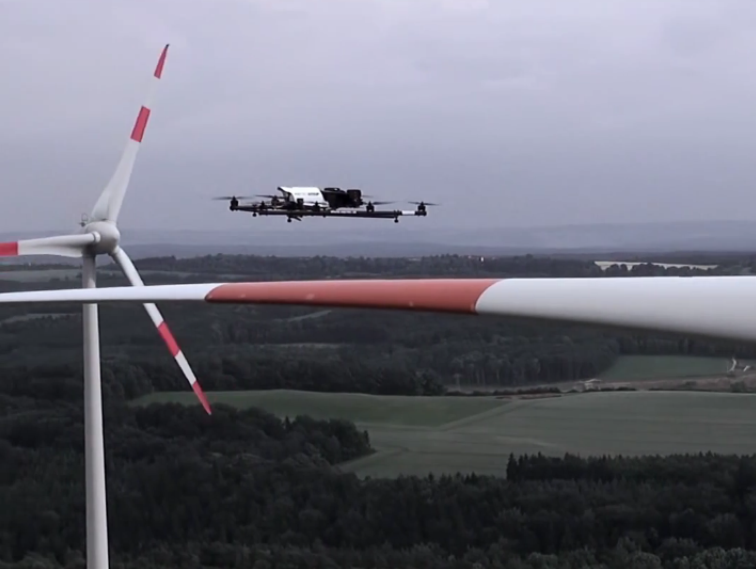
\includegraphics[width=1\textwidth]{images/mav_wind_turbine.png}\\
	\tiny{AscTec Falcon 8 at wind turbine inspection, \cite{www:asctecinspect}} 
\end{minipage}

\vspace*{\fill}
\clearpage

\ETHslide
\section*{Overview}
\tableofcontents
\clearpage

\addcontentsline{toc}{section}{Modelling}
\ETHslide
\section*{Equations of Motion}
%\addcontentsline{toc}{section}{Modelling}
\vspace*{\fill}

%\centering
%\def\svgwidth{0.45\textwidth}
%\tiny{
%\input{images/hexa.pdf_tex}
%}
%
%\normalsize{	
%\begin{align}
%m \cdot \mathbf{a} &= \rotWB \sum_{i=1}^n \underbrace{\left(\mathbf{F}_{T,i} + \mathbf{F}_{D,i} \right)}_{=:\mathbf{F}_i} + \mathbf{F}_G \\
%\mathbf{J} \cdot  \mathbf{\dot{\boldsymbol{\omega}}} + \boldsymbol{\omega} \times \mathbf{J} \cdot \boldsymbol{\omega} &= \sum_{i=1}^n \left( \mathbf{M}_{R,i}+ \mathbf{M}_{D,i} + \mathbf{F}_i \times \mathbf{l}_i \right)
%\end{align}
%}

\begin{minipage}{0.5\textwidth}
	\centering
    \def\svgwidth{1\textwidth}
    \tiny{
	\input{images/hexa.pdf_tex}}
\end{minipage}
\begin{minipage}{0.49\textwidth}
\footnotesize{
\begin{align}
m \cdot \mathbf{a} &= \rotWB \sum_{i=1}^n \underbrace{\left(\mathbf{F}_{T,i} + \mathbf{F}_{D,i} \right)}_{=:\mathbf{F}_i} + \mathbf{F}_G \nonumber \\
\mathbf{J} \cdot  \mathbf{\dot{\boldsymbol{\omega}}} + \boldsymbol{\omega} \times \mathbf{J} \cdot \boldsymbol{\omega} &= \sum_{i=1}^n \left( \mathbf{M}_{R,i}+ \mathbf{M}_{D,i} + \mathbf{F}_i \times \mathbf{l}_i \right) \nonumber
\end{align}}
\end{minipage}

\vspace*{\fill}
\clearpage
\ETHslide
\section*{Wind Drag}
%\addcontentsline{toc}{section}{Wind Drag}
\vspace*{\fill}


\begin{minipage}{0.5\textwidth}
\begin{itemize}
	\item[\ETHitem] Air speed
	\begin{itemize}
	\item[\ETHitem] $\boldsymbol{\nu} = \mathbf{v}-\mathbf{w}  $
	\end{itemize}
	\item[\ETHitem] Area drag \cite{Schiano2014}
	\begin{itemize}
	\item[\ETHitem] $\mathbf{F}_A = -\frac{1}{2} C_A \rho \norm{\boldsymbol{\nu}}_2 \boldsymbol{\nu}  $
	\end{itemize}
	\item[\ETHitem] Rotor drag
	\begin{itemize}
	\item[\ETHitem] $\mathbf{F}_D =  -\sum_{i=1}^n \omega_i \cdot  C_D \cdot \boldsymbol{\nu}^\perp$
	\end{itemize}
\end{itemize}
\end{minipage}
\begin{minipage}{0.49\textwidth}
	\centering
	\tiny{
	% This file was created by matlab2tikz.
% Minimal pgfplots version: 1.3
%
%The latest updates can be retrieved from
%  http://www.mathworks.com/matlabcentral/fileexchange/22022-matlab2tikz
%where you can also make suggestions and rate matlab2tikz.
%
\definecolor{mycolor1}{rgb}{0.00000,0.44700,0.74100}%
\definecolor{mycolor2}{rgb}{0.85000,0.32500,0.09800}%
%
\begin{tikzpicture}

\begin{axis}[%
width=0.95092\figurewidth,
height=\figureheight,
at={(0\figurewidth,0\figureheight)},
scale only axis,
xmin=0,
xmax=20,
xlabel={Wind velocity $[\si{\metre\per\second}]$},
ymin=0,
ymax=6,
ytick={0, 1, 2, 3, 4, 5},
ylabel={Drag force [\si{\newton}]},
legend style={legend cell align=left,align=left,draw=white!15!black}
]
\addplot [color=mycolor1,solid]
  table[row sep=crcr]{%
0	0\\
0.02002002002002	4.90981471962453e-06\\
0.04004004004004	1.96392588784981e-05\\
0.0600600600600601	4.41883324766208e-05\\
0.0800800800800801	7.85570355139925e-05\\
0.1001001001001	0.000122745367990613\\
0.12012012012012	0.000176753329906483\\
0.14014014014014	0.000240580921261602\\
0.16016016016016	0.00031422814205597\\
0.18018018018018	0.000397694992289587\\
0.2002002002002	0.000490981471962453\\
0.22022022022022	0.000594087581074568\\
0.24024024024024	0.000707013319625932\\
0.26026026026026	0.000829758687616546\\
0.28028028028028	0.000962323685046408\\
0.3003003003003	0.00110470831191552\\
0.32032032032032	0.00125691256822388\\
0.34034034034034	0.00141893645397149\\
0.36036036036036	0.00159077996915835\\
0.38038038038038	0.00177244311378446\\
0.4004004004004	0.00196392588784981\\
0.42042042042042	0.00216522829135442\\
0.44044044044044	0.00237635032429827\\
0.46046046046046	0.00259729198668138\\
0.48048048048048	0.00282805327850373\\
0.500500500500501	0.00306863419976533\\
0.520520520520521	0.00331903475046618\\
0.540540540540541	0.00357925493060628\\
0.560560560560561	0.00384929474018563\\
0.580580580580581	0.00412915417920423\\
0.600600600600601	0.00441883324766208\\
0.620620620620621	0.00471833194555917\\
0.640640640640641	0.00502765027289552\\
0.660660660660661	0.00534678822967111\\
0.680680680680681	0.00567574581588596\\
0.700700700700701	0.00601452303154005\\
0.720720720720721	0.00636311987663339\\
0.740740740740741	0.00672153635116598\\
0.760760760760761	0.00708977245513782\\
0.780780780780781	0.00746782818854891\\
0.800800800800801	0.00785570355139925\\
0.820820820820821	0.00825339854368884\\
0.840840840840841	0.00866091316541767\\
0.860860860860861	0.00907824741658575\\
0.880880880880881	0.00950540129719309\\
0.900900900900901	0.00994237480723967\\
0.920920920920921	0.0103891679467255\\
0.940940940940941	0.0108457807156506\\
0.960960960960961	0.0113122131140149\\
0.980980980980981	0.0117884651418185\\
1.001001001001	0.0122745367990613\\
1.02102102102102	0.0127704280857434\\
1.04104104104104	0.0132761390018647\\
1.06106106106106	0.0137916695474253\\
1.08108108108108	0.0143170197224251\\
1.1011011011011	0.0148521895268642\\
1.12112112112112	0.0153971789607425\\
1.14114114114114	0.0159519880240601\\
1.16116116116116	0.0165166167168169\\
1.18118118118118	0.017091065039013\\
1.2012012012012	0.0176753329906483\\
1.22122122122122	0.0182694205717229\\
1.24124124124124	0.0188733277822367\\
1.26126126126126	0.0194870546221898\\
1.28128128128128	0.0201106010915821\\
1.3013013013013	0.0207439671904136\\
1.32132132132132	0.0213871529186845\\
1.34134134134134	0.0220401582763945\\
1.36136136136136	0.0227029832635438\\
1.38138138138138	0.0233756278801324\\
1.4014014014014	0.0240580921261602\\
1.42142142142142	0.0247503760016273\\
1.44144144144144	0.0254524795065336\\
1.46146146146146	0.0261644026408791\\
1.48148148148148	0.0268861454046639\\
1.5015015015015	0.027617707797888\\
1.52152152152152	0.0283590898205513\\
1.54154154154154	0.0291102914726538\\
1.56156156156156	0.0298713127541956\\
1.58158158158158	0.0306421536651767\\
1.6016016016016	0.031422814205597\\
1.62162162162162	0.0322132943754565\\
1.64164164164164	0.0330135941747553\\
1.66166166166166	0.0338237136034934\\
1.68168168168168	0.0346436526616707\\
1.7017017017017	0.0354734113492872\\
1.72172172172172	0.036312989666343\\
1.74174174174174	0.0371623876128381\\
1.76176176176176	0.0380216051887724\\
1.78178178178178	0.0388906423941459\\
1.8018018018018	0.0397694992289587\\
1.82182182182182	0.0406581756932107\\
1.84184184184184	0.041556671786902\\
1.86186186186186	0.0424649875100326\\
1.88188188188188	0.0433831228626023\\
1.9019019019019	0.0443110778446114\\
1.92192192192192	0.0452488524560597\\
1.94194194194194	0.0461964466969472\\
1.96196196196196	0.047153860567274\\
1.98198198198198	0.04812109406704\\
2.002002002002	0.0490981471962453\\
2.02202202202202	0.0500850199548898\\
2.04204204204204	0.0510817123429736\\
2.06206206206206	0.0520882243604966\\
2.08208208208208	0.0531045560074589\\
2.1021021021021	0.0541307072838604\\
2.12212212212212	0.0551666781897012\\
2.14214214214214	0.0562124687249812\\
2.16216216216216	0.0572680788897005\\
2.18218218218218	0.058333508683859\\
2.2022022022022	0.0594087581074568\\
2.22222222222222	0.0604938271604938\\
2.24224224224224	0.0615887158429701\\
2.26226226226226	0.0626934241548856\\
2.28228228228228	0.0638079520962404\\
2.3023023023023	0.0649322996670344\\
2.32232232232232	0.0660664668672677\\
2.34234234234234	0.0672104536969402\\
2.36236236236236	0.068364260156052\\
2.38238238238238	0.069527886244603\\
2.4024024024024	0.0707013319625932\\
2.42242242242242	0.0718845973100227\\
2.44244244244244	0.0730776822868915\\
2.46246246246246	0.0742805868931995\\
2.48248248248248	0.0754933111289468\\
2.5025025025025	0.0767158549941333\\
2.52252252252252	0.077948218488759\\
2.54254254254254	0.079190401612824\\
2.56256256256256	0.0804424043663283\\
2.58258258258258	0.0817042267492718\\
2.6026026026026	0.0829758687616546\\
2.62262262262262	0.0842573304034765\\
2.64264264264264	0.0855486116747378\\
2.66266266266266	0.0868497125754383\\
2.68268268268268	0.088160633105578\\
2.7027027027027	0.089481373265157\\
2.72272272272272	0.0908119330541753\\
2.74274274274274	0.0921523124726328\\
2.76276276276276	0.0935025115205295\\
2.78278278278278	0.0948625301978655\\
2.8028028028028	0.0962323685046408\\
2.82282282282282	0.0976120264408553\\
2.84284284284284	0.099001504006509\\
2.86286286286286	0.100400801201602\\
2.88288288288288	0.101809918026134\\
2.9029029029029	0.103228854480106\\
2.92292292292292	0.104657610563516\\
2.94294294294294	0.106096186276366\\
2.96296296296296	0.107544581618656\\
2.98298298298298	0.109002796590384\\
3.003003003003	0.110470831191552\\
3.02302302302302	0.111948685422159\\
3.04304304304304	0.113436359282205\\
3.06306306306306	0.114933852771691\\
3.08308308308308	0.116441165890615\\
3.1031031031031	0.117958298638979\\
3.12312312312312	0.119485251016783\\
3.14314314314314	0.121022023024025\\
3.16316316316316	0.122568614660707\\
3.18318318318318	0.124125025926828\\
3.2032032032032	0.125691256822388\\
3.22322322322322	0.127267307347387\\
3.24324324324324	0.128853177501826\\
3.26326326326326	0.130448867285704\\
3.28328328328328	0.132054376699021\\
3.3033033033033	0.133669705741778\\
3.32332332332332	0.135294854413974\\
3.34334334334334	0.136929822715609\\
3.36336336336336	0.138574610646683\\
3.38338338338338	0.140229218207196\\
3.4034034034034	0.141893645397149\\
3.42342342342342	0.143567892216541\\
3.44344344344344	0.145251958665372\\
3.46346346346346	0.146945844743643\\
3.48348348348348	0.148649550451352\\
3.5035035035035	0.150363075788501\\
3.52352352352352	0.152086420755089\\
3.54354354354354	0.153819585351117\\
3.56356356356356	0.155562569576584\\
3.58358358358358	0.15731537343149\\
3.6036036036036	0.159077996915835\\
3.62362362362362	0.160850440029619\\
3.64364364364364	0.162632702772843\\
3.66366366366366	0.164424785145506\\
3.68368368368368	0.166226687147608\\
3.7037037037037	0.16803840877915\\
3.72372372372372	0.16985995004013\\
3.74374374374374	0.17169131093055\\
3.76376376376376	0.173532491450409\\
3.78378378378378	0.175383491599708\\
3.8038038038038	0.177244311378446\\
3.82382382382382	0.179114950786622\\
3.84384384384384	0.180995409824239\\
3.86386386386386	0.182885688491294\\
3.88388388388388	0.184785786787789\\
3.9039039039039	0.186695704713723\\
3.92392392392392	0.188615442269096\\
3.94394394394394	0.190544999453908\\
3.96396396396396	0.19248437626816\\
3.98398398398398	0.194433572711851\\
4.004004004004	0.196392588784981\\
4.02402402402402	0.198361424487551\\
4.04404404404404	0.200340079819559\\
4.06406406406406	0.202328554781007\\
4.08408408408408	0.204326849371894\\
4.1041041041041	0.206334963592221\\
4.12412412412412	0.208352897441987\\
4.14414414414414	0.210380650921192\\
4.16416416416416	0.212418224029836\\
4.18418418418418	0.214465616767919\\
4.2042042042042	0.216522829135442\\
4.22422422422422	0.218589861132404\\
4.24424424424424	0.220666712758805\\
4.26426426426426	0.222753384014645\\
4.28428428428428	0.224849874899925\\
4.3043043043043	0.226956185414644\\
4.32432432432432	0.229072315558802\\
4.34434434434434	0.2311982653324\\
4.36436436436436	0.233334034735436\\
4.38438438438438	0.235479623767912\\
4.4044044044044	0.237635032429827\\
4.42442442442442	0.239800260721182\\
4.44444444444444	0.241975308641975\\
4.46446446446446	0.244160176192208\\
4.48448448448448	0.24635486337188\\
4.5045045045045	0.248559370180992\\
4.52452452452452	0.250773696619542\\
4.54454454454454	0.252997842687532\\
4.56456456456456	0.255231808384962\\
4.58458458458458	0.25747559371183\\
4.6046046046046	0.259729198668138\\
4.62462462462462	0.261992623253885\\
4.64464464464464	0.264265867469071\\
4.66466466466466	0.266548931313696\\
4.68468468468468	0.268841814787761\\
4.7047047047047	0.271144517891265\\
4.72472472472472	0.273457040624208\\
4.74474474474474	0.27577938298659\\
4.76476476476476	0.278111544978412\\
4.78478478478478	0.280453526599673\\
4.8048048048048	0.282805327850373\\
4.82482482482482	0.285166948730512\\
4.84484484484484	0.287538389240091\\
4.86486486486486	0.289919649379109\\
4.88488488488488	0.292310729147566\\
4.9049049049049	0.294711628545462\\
4.92492492492492	0.297122347572798\\
4.94494494494494	0.299542886229573\\
4.96496496496496	0.301973244515787\\
4.98498498498498	0.30441342243144\\
5.00500500500501	0.306863419976533\\
5.02502502502503	0.309323237151065\\
5.04504504504505	0.311792873955036\\
5.06506506506507	0.314272330388447\\
5.08508508508509	0.316761606451296\\
5.10510510510511	0.319260702143585\\
5.12512512512513	0.321769617465313\\
5.14514514514515	0.324288352416481\\
5.16516516516517	0.326816906997087\\
5.18518518518519	0.329355281207133\\
5.20520520520521	0.331903475046618\\
5.22522522522523	0.334461488515543\\
5.24524524524525	0.337029321613906\\
5.26526526526527	0.339606974341709\\
5.28528528528529	0.342194446698951\\
5.30530530530531	0.344791738685633\\
5.32532532532533	0.347398850301753\\
5.34534534534535	0.350015781547313\\
5.36536536536537	0.352642532422312\\
5.38538538538539	0.355279102926751\\
5.40540540540541	0.357925493060628\\
5.42542542542543	0.360581702823945\\
5.44544544544545	0.363247732216701\\
5.46546546546547	0.365923581238897\\
5.48548548548549	0.368609249890531\\
5.50550550550551	0.371304738171605\\
5.52552552552553	0.374010046082118\\
5.54554554554555	0.37672517362207\\
5.56556556556557	0.379450120791462\\
5.58558558558559	0.382184887590293\\
5.60560560560561	0.384929474018563\\
5.62562562562563	0.387683880076272\\
5.64564564564565	0.390448105763421\\
5.66566566566567	0.393222151080009\\
5.68568568568569	0.396006016026036\\
5.70570570570571	0.398799700601502\\
5.72572572572573	0.401603204806408\\
5.74574574574575	0.404416528640753\\
5.76576576576577	0.407239672104537\\
5.78578578578579	0.41007263519776\\
5.80580580580581	0.412915417920423\\
5.82582582582583	0.415768020272525\\
5.84584584584585	0.418630442254066\\
5.86586586586587	0.421502683865046\\
5.88588588588589	0.424384745105466\\
5.90590590590591	0.427276625975325\\
5.92592592592593	0.430178326474623\\
5.94594594594595	0.43308984660336\\
5.96596596596597	0.436011186361537\\
5.98598598598599	0.438942345749153\\
6.00600600600601	0.441883324766208\\
6.02602602602603	0.444834123412702\\
6.04604604604605	0.447794741688636\\
6.06606606606607	0.450765179594008\\
6.08608608608609	0.45374543712882\\
6.10610610610611	0.456735514293072\\
6.12612612612613	0.459735411086762\\
6.14614614614615	0.462745127509892\\
6.16616616616617	0.465764663562461\\
6.18618618618619	0.46879401924447\\
6.20620620620621	0.471833194555917\\
6.22622622622623	0.474882189496804\\
6.24624624624625	0.47794100406713\\
6.26626626626627	0.481009638266896\\
6.28628628628629	0.4840880920961\\
6.30630630630631	0.487176365554744\\
6.32632632632633	0.490274458642827\\
6.34634634634635	0.493382371360349\\
6.36636636636637	0.496500103707311\\
6.38638638638639	0.499627655683712\\
6.40640640640641	0.502765027289552\\
6.42642642642643	0.505912218524831\\
6.44644644644645	0.50906922938955\\
6.46646646646647	0.512236059883708\\
6.48648648648649	0.515412710007305\\
6.50650650650651	0.518599179760341\\
6.52652652652653	0.521795469142816\\
6.54654654654655	0.525001578154731\\
6.56656656656657	0.528217506796085\\
6.58658658658659	0.531443255066879\\
6.60660660660661	0.534678822967111\\
6.62662662662663	0.537924210496783\\
6.64664664664665	0.541179417655894\\
6.66666666666667	0.544444444444445\\
6.68668668668669	0.547719290862434\\
6.70670670670671	0.551003956909863\\
6.72672672672673	0.554298442586731\\
6.74674674674675	0.557602747893038\\
6.76676676676677	0.560916872828785\\
6.78678678678679	0.564240817393971\\
6.80680680680681	0.567574581588596\\
6.82682682682683	0.57091816541266\\
6.84684684684685	0.574271568866163\\
6.86686686686687	0.577634791949106\\
6.88688688688689	0.581007834661488\\
6.90690690690691	0.58439069700331\\
6.92692692692693	0.58778337897457\\
6.94694694694695	0.59118588057527\\
6.96696696696697	0.594598201805409\\
6.98698698698699	0.598020342664987\\
7.00700700700701	0.601452303154005\\
7.02702702702703	0.604894083272462\\
7.04704704704705	0.608345683020358\\
7.06706706706707	0.611807102397693\\
7.08708708708709	0.615278341404468\\
7.10710710710711	0.618759400040681\\
7.12712712712713	0.622250278306334\\
7.14714714714715	0.625750976201427\\
7.16716716716717	0.629261493725958\\
7.18718718718719	0.632781830879929\\
7.20720720720721	0.636311987663339\\
7.22722722722723	0.639851964076188\\
7.24724724724725	0.643401760118477\\
7.26726726726727	0.646961375790205\\
7.28728728728729	0.650530811091372\\
7.30730730730731	0.654110066021978\\
7.32732732732733	0.657699140582024\\
7.34734734734735	0.661298034771508\\
7.36736736736737	0.664906748590432\\
7.38738738738739	0.668525282038796\\
7.40740740740741	0.672153635116598\\
7.42742742742743	0.67579180782384\\
7.44744744744745	0.679439800160521\\
7.46746746746747	0.683097612126641\\
7.48748748748749	0.686765243722201\\
7.50750750750751	0.690442694947199\\
7.52752752752753	0.694129965801638\\
7.54754754754755	0.697827056285515\\
7.56756756756757	0.701533966398831\\
7.58758758758759	0.705250696141587\\
7.60760760760761	0.708977245513782\\
7.62762762762763	0.712713614515416\\
7.64764764764765	0.71645980314649\\
7.66766766766767	0.720215811407003\\
7.68768768768769	0.723981639296955\\
7.70770770770771	0.727757286816346\\
7.72772772772773	0.731542753965176\\
7.74774774774775	0.735338040743446\\
7.76776776776777	0.739143147151155\\
7.78778778778779	0.742958073188303\\
7.80780780780781	0.746782818854891\\
7.82782782782783	0.750617384150918\\
7.84784784784785	0.754461769076384\\
7.86786786786787	0.758315973631289\\
7.88788788788789	0.762179997815634\\
7.90790790790791	0.766053841629417\\
7.92792792792793	0.76993750507264\\
7.94794794794795	0.773830988145302\\
7.96796796796797	0.777734290847404\\
7.98798798798799	0.781647413178945\\
8.00800800800801	0.785570355139925\\
8.02802802802803	0.789503116730344\\
8.04804804804805	0.793445697950203\\
8.06806806806807	0.7973980987995\\
8.08808808808809	0.801360319278237\\
8.10810810810811	0.805332359386414\\
8.12812812812813	0.809314219124029\\
8.14814814814815	0.813305898491084\\
8.16816816816817	0.817307397487578\\
8.18818818818819	0.821318716113511\\
8.20820820820821	0.825339854368884\\
8.22822822822823	0.829370812253695\\
8.24824824824825	0.833411589767946\\
8.26826826826827	0.837462186911636\\
8.28828828828829	0.841522603684766\\
8.30830830830831	0.845592840087335\\
8.32832832832833	0.849672896119343\\
8.34834834834835	0.85376277178079\\
8.36836836836837	0.857862467071676\\
8.38838838838839	0.861971981992002\\
8.40840840840841	0.866091316541767\\
8.42842842842843	0.870220470720971\\
8.44844844844845	0.874359444529615\\
8.46846846846847	0.878508237967698\\
8.48848848848849	0.88266685103522\\
8.50850850850851	0.886835283732181\\
8.52852852852853	0.891013536058581\\
8.54854854854855	0.895201608014421\\
8.56856856856857	0.8993994995997\\
8.58858858858859	0.903607210814418\\
8.60860860860861	0.907824741658576\\
8.62862862862863	0.912052092132172\\
8.64864864864865	0.916289262235208\\
8.66866866866867	0.920536251967683\\
8.68868868868869	0.924793061329598\\
8.70870870870871	0.929059690320952\\
8.72872872872873	0.933336138941745\\
8.74874874874875	0.937622407191977\\
8.76876876876877	0.941918495071648\\
8.78878878878879	0.946224402580759\\
8.80880880880881	0.950540129719309\\
8.82882882882883	0.954865676487298\\
8.84884884884885	0.959201042884727\\
8.86886886886887	0.963546228911594\\
8.88888888888889	0.967901234567901\\
8.90890890890891	0.972266059853648\\
8.92892892892893	0.976640704768833\\
8.94894894894895	0.981025169313458\\
8.96896896896897	0.985419453487522\\
8.98898898898899	0.989823557291025\\
9.00900900900901	0.994237480723967\\
9.02902902902903	0.998661223786349\\
9.04904904904905	1.00309478647817\\
9.06906906906907	1.00753816879943\\
9.08908908908909	1.01199137075013\\
9.10910910910911	1.01645439233027\\
9.12912912912913	1.02092723353985\\
9.14914914914915	1.02540989437886\\
9.16916916916917	1.02990237484732\\
9.18918918918919	1.03440467494522\\
9.20920920920921	1.03891679467255\\
9.22922922922923	1.04343873402932\\
9.24924924924925	1.04797049301554\\
9.26926926926927	1.05251207163119\\
9.28928928928929	1.05706346987628\\
9.30930930930931	1.06162468775081\\
9.32932932932933	1.06619572525478\\
9.34934934934935	1.07077658238819\\
9.36936936936937	1.07536725915104\\
9.38938938938939	1.07996775554333\\
9.40940940940941	1.08457807156506\\
9.42942942942943	1.08919820721623\\
9.44944944944945	1.09382816249683\\
9.46946946946947	1.09846793740688\\
9.48948948948949	1.10311753194636\\
9.50950950950951	1.10777694611528\\
9.52952952952953	1.11244617991365\\
9.54954954954955	1.11712523334145\\
9.56956956956957	1.12181410639869\\
9.58958958958959	1.12651279908537\\
9.60960960960961	1.13122131140149\\
9.62962962962963	1.13593964334705\\
9.64964964964965	1.14066779492205\\
9.66966966966967	1.14540576612649\\
9.68968968968969	1.15015355696036\\
9.70970970970971	1.15491116742368\\
9.72972972972973	1.15967859751644\\
9.74974974974975	1.16445584723863\\
9.76976976976977	1.16924291659026\\
9.78978978978979	1.17403980557134\\
9.80980980980981	1.17884651418185\\
9.82982982982983	1.1836630424218\\
9.84984984984985	1.18848939029119\\
9.86986986986987	1.19332555779002\\
9.88988988988989	1.19817154491829\\
9.90990990990991	1.203027351676\\
9.92992992992993	1.20789297806315\\
9.94994994994995	1.21276842407974\\
9.96996996996997	1.21765368972576\\
9.98998998998999	1.22254877500123\\
10.01001001001	1.22745367990613\\
10.03003003003	1.23236840444048\\
10.0500500500501	1.23729294860426\\
10.0700700700701	1.24222731239748\\
10.0900900900901	1.24717149582014\\
10.1101101101101	1.25212549887225\\
10.1301301301301	1.25708932155379\\
10.1501501501502	1.26206296386477\\
10.1701701701702	1.26704642580518\\
10.1901901901902	1.27203970737504\\
10.2102102102102	1.27704280857434\\
10.2302302302302	1.28205572940308\\
10.2502502502503	1.28707846986125\\
10.2702702702703	1.29211102994887\\
10.2902902902903	1.29715340966592\\
10.3103103103103	1.30220560901242\\
10.3303303303303	1.30726762798835\\
10.3503503503504	1.31233946659372\\
10.3703703703704	1.31742112482853\\
10.3903903903904	1.32251260269278\\
10.4104104104104	1.32761390018647\\
10.4304304304304	1.3327250173096\\
10.4504504504505	1.33784595406217\\
10.4704704704705	1.34297671044418\\
10.4904904904905	1.34811728645562\\
10.5105105105105	1.35326768209651\\
10.5305305305305	1.35842789736684\\
10.5505505505506	1.3635979322666\\
10.5705705705706	1.3687777867958\\
10.5905905905906	1.37396746095445\\
10.6106106106106	1.37916695474253\\
10.6306306306306	1.38437626816005\\
10.6506506506507	1.38959540120701\\
10.6706706706707	1.39482435388341\\
10.6906906906907	1.40006312618925\\
10.7107107107107	1.40531171812453\\
10.7307307307307	1.41057012968925\\
10.7507507507508	1.41583836088341\\
10.7707707707708	1.421116411707\\
10.7907907907908	1.42640428216004\\
10.8108108108108	1.43170197224251\\
10.8308308308308	1.43700948195443\\
10.8508508508509	1.44232681129578\\
10.8708708708709	1.44765396026657\\
10.8908908908909	1.4529909288668\\
10.9109109109109	1.45833771709648\\
10.9309309309309	1.46369432495559\\
10.950950950951	1.46906075244414\\
10.970970970971	1.47443699956212\\
10.990990990991	1.47982306630955\\
11.011011011011	1.48521895268642\\
11.031031031031	1.49062465869273\\
11.0510510510511	1.49604018432847\\
11.0710710710711	1.50146552959366\\
11.0910910910911	1.50690069448828\\
11.1111111111111	1.51234567901235\\
11.1311311311311	1.51780048316585\\
11.1511511511512	1.52326510694879\\
11.1711711711712	1.52873955036117\\
11.1911911911912	1.53422381340299\\
11.2112112112112	1.53971789607425\\
11.2312312312312	1.54522179837495\\
11.2512512512513	1.55073552030509\\
11.2712712712713	1.55625906186467\\
11.2912912912913	1.56179242305368\\
11.3113113113113	1.56733560387214\\
11.3313313313313	1.57288860432004\\
11.3513513513514	1.57845142439737\\
11.3713713713714	1.58402406410414\\
11.3913913913914	1.58960652344036\\
11.4114114114114	1.59519880240601\\
11.4314314314314	1.6008009010011\\
11.4514514514515	1.60641281922563\\
11.4714714714715	1.6120345570796\\
11.4914914914915	1.61766611456301\\
11.5115115115115	1.62330749167586\\
11.5315315315315	1.62895868841815\\
11.5515515515516	1.63461970478987\\
11.5715715715716	1.64029054079104\\
11.5915915915916	1.64597119642165\\
11.6116116116116	1.65166167168169\\
11.6316316316316	1.65736196657118\\
11.6516516516517	1.6630720810901\\
11.6716716716717	1.66879201523846\\
11.6916916916917	1.67452176901626\\
11.7117117117117	1.6802613424235\\
11.7317317317317	1.68601073546018\\
11.7517517517518	1.6917699481263\\
11.7717717717718	1.69753898042186\\
11.7917917917918	1.70331783234686\\
11.8118118118118	1.7091065039013\\
11.8318318318318	1.71490499508518\\
11.8518518518519	1.72071330589849\\
11.8718718718719	1.72653143634125\\
11.8918918918919	1.73235938641344\\
11.9119119119119	1.73819715611507\\
11.9319319319319	1.74404474544615\\
11.951951951952	1.74990215440666\\
11.971971971972	1.75576938299661\\
11.991991991992	1.761646431216\\
12.012012012012	1.76753329906483\\
12.032032032032	1.7734299865431\\
12.0520520520521	1.77933649365081\\
12.0720720720721	1.78525282038796\\
12.0920920920921	1.79117896675454\\
12.1121121121121	1.79711493275057\\
12.1321321321321	1.80306071837603\\
12.1521521521522	1.80901632363094\\
12.1721721721722	1.81498174851528\\
12.1921921921922	1.82095699302906\\
12.2122122122122	1.82694205717229\\
12.2322322322322	1.83293694094495\\
12.2522522522523	1.83894164434705\\
12.2722722722723	1.84495616737859\\
12.2922922922923	1.85098051003957\\
12.3123123123123	1.85701467232999\\
12.3323323323323	1.86305865424985\\
12.3523523523524	1.86911245579914\\
12.3723723723724	1.87517607697788\\
12.3923923923924	1.88124951778605\\
12.4124124124124	1.88733277822367\\
12.4324324324324	1.89342585829072\\
12.4524524524525	1.89952875798722\\
12.4724724724725	1.90564147731315\\
12.4924924924925	1.91176401626852\\
12.5125125125125	1.91789637485333\\
12.5325325325325	1.92403855306758\\
12.5525525525526	1.93019055091127\\
12.5725725725726	1.9363523683844\\
12.5925925925926	1.94252400548697\\
12.6126126126126	1.94870546221898\\
12.6326326326326	1.95489673858042\\
12.6526526526527	1.96109783457131\\
12.6726726726727	1.96730875019163\\
12.6926926926927	1.9735294854414\\
12.7127127127127	1.9797600403206\\
12.7327327327327	1.98600041482924\\
12.7527527527528	1.99225060896733\\
12.7727727727728	1.99851062273485\\
12.7927927927928	2.00478045613181\\
12.8128128128128	2.01106010915821\\
12.8328328328328	2.01734958181405\\
12.8528528528529	2.02364887409933\\
12.8728728728729	2.02995798601404\\
12.8928928928929	2.0362769175582\\
12.9129129129129	2.0426056687318\\
12.9329329329329	2.04894423953483\\
12.952952952953	2.05529262996731\\
12.972972972973	2.06165084002922\\
12.992992992993	2.06801886972057\\
13.013013013013	2.07439671904136\\
13.033033033033	2.0807843879916\\
13.0530530530531	2.08718187657127\\
13.0730730730731	2.09358918478038\\
13.0930930930931	2.10000631261893\\
13.1131131131131	2.10643326008691\\
13.1331331331331	2.11287002718434\\
13.1531531531532	2.11931661391121\\
13.1731731731732	2.12577302026752\\
13.1931931931932	2.13223924625326\\
13.2132132132132	2.13871529186845\\
13.2332332332332	2.14520115711307\\
13.2532532532533	2.15169684198713\\
13.2732732732733	2.15820234649064\\
13.2932932932933	2.16471767062358\\
13.3133133133133	2.17124281438596\\
13.3333333333333	2.17777777777778\\
13.3533533533534	2.18432256079904\\
13.3733733733734	2.19087716344974\\
13.3933933933934	2.19744158572987\\
13.4134134134134	2.20401582763945\\
13.4334334334334	2.21059988917847\\
13.4534534534535	2.21719377034692\\
13.4734734734735	2.22379747114482\\
13.4934934934935	2.23041099157215\\
13.5135135135135	2.23703433162893\\
13.5335335335335	2.24366749131514\\
13.5535535535536	2.25031047063079\\
13.5735735735736	2.25696326957588\\
13.5935935935936	2.26362588815041\\
13.6136136136136	2.27029832635438\\
13.6336336336336	2.27698058418779\\
13.6536536536537	2.28367266165064\\
13.6736736736737	2.29037455874293\\
13.6936936936937	2.29708627546465\\
13.7137137137137	2.30380781181582\\
13.7337337337337	2.31053916779643\\
13.7537537537538	2.31728034340647\\
13.7737737737738	2.32403133864595\\
13.7937937937938	2.33079215351488\\
13.8138138138138	2.33756278801324\\
13.8338338338338	2.34434324214104\\
13.8538538538539	2.35113351589828\\
13.8738738738739	2.35793360928496\\
13.8938938938939	2.36474352230108\\
13.9139139139139	2.37156325494664\\
13.9339339339339	2.37839280722164\\
13.953953953954	2.38523217912607\\
13.973973973974	2.39208137065995\\
13.993993993994	2.39894038182326\\
14.014014014014	2.40580921261602\\
14.034034034034	2.41268786303821\\
14.0540540540541	2.41957633308985\\
14.0740740740741	2.42647462277092\\
14.0940940940941	2.43338273208143\\
14.1141141141141	2.44030066102138\\
14.1341341341341	2.44722840959077\\
14.1541541541542	2.4541659777896\\
14.1741741741742	2.46111336561787\\
14.1941941941942	2.46807057307558\\
14.2142142142142	2.47503760016273\\
14.2342342342342	2.48201444687931\\
14.2542542542543	2.48900111322534\\
14.2742742742743	2.4959975992008\\
14.2942942942943	2.50300390480571\\
14.3143143143143	2.51002003004005\\
14.3343343343343	2.51704597490383\\
14.3543543543544	2.52408173939705\\
14.3743743743744	2.53112732351972\\
14.3943943943944	2.53818272727182\\
14.4144144144144	2.54524795065336\\
14.4344344344344	2.55232299366434\\
14.4544544544545	2.55940785630475\\
14.4744744744745	2.56650253857461\\
14.4944944944945	2.57360704047391\\
14.5145145145145	2.58072136200264\\
14.5345345345345	2.58784550316082\\
14.5545545545546	2.59497946394843\\
14.5745745745746	2.60212324436549\\
14.5945945945946	2.60927684441198\\
14.6146146146146	2.61644026408791\\
14.6346346346346	2.62361350339328\\
14.6546546546547	2.63079656232809\\
14.6746746746747	2.63798944089234\\
14.6946946946947	2.64519213908603\\
14.7147147147147	2.65240465690916\\
14.7347347347347	2.65962699436173\\
14.7547547547548	2.66685915144374\\
14.7747747747748	2.67410112815518\\
14.7947947947948	2.68135292449607\\
14.8148148148148	2.68861454046639\\
14.8348348348348	2.69588597606616\\
14.8548548548549	2.70316723129536\\
14.8748748748749	2.710458306154\\
14.8948948948949	2.71775920064208\\
14.9149149149149	2.7250699147596\\
14.9349349349349	2.73239044850656\\
14.954954954955	2.73972080188296\\
14.974974974975	2.7470609748888\\
14.994994994995	2.75441096752408\\
15.015015015015	2.7617707797888\\
15.035035035035	2.76914041168295\\
15.0550550550551	2.77651986320655\\
15.0750750750751	2.78390913435959\\
15.0950950950951	2.79130822514206\\
15.1151151151151	2.79871713555397\\
15.1351351351351	2.80613586559533\\
15.1551551551552	2.81356441526612\\
15.1751751751752	2.82100278456635\\
15.1951951951952	2.82845097349602\\
15.2152152152152	2.83590898205513\\
15.2352352352352	2.84337681024368\\
15.2552552552553	2.85085445806167\\
15.2752752752753	2.85834192550909\\
15.2952952952953	2.86583921258596\\
15.3153153153153	2.87334631929227\\
15.3353353353353	2.88086324562801\\
15.3553553553554	2.88838999159319\\
15.3753753753754	2.89592655718782\\
15.3953953953954	2.90347294241188\\
15.4154154154154	2.91102914726538\\
15.4354354354354	2.91859517174832\\
15.4554554554555	2.92617101586071\\
15.4754754754755	2.93375667960253\\
15.4954954954955	2.94135216297378\\
15.5155155155155	2.94895746597448\\
15.5355355355355	2.95657258860462\\
15.5555555555556	2.9641975308642\\
15.5755755755756	2.97183229275321\\
15.5955955955956	2.97947687427167\\
15.6156156156156	2.98713127541956\\
15.6356356356356	2.9947954961969\\
15.6556556556557	3.00246953660367\\
15.6756756756757	3.01015339663988\\
15.6956956956957	3.01784707630553\\
15.7157157157157	3.02555057560063\\
15.7357357357357	3.03326389452516\\
15.7557557557558	3.04098703307913\\
15.7757757757758	3.04871999126253\\
15.7957957957958	3.05646276907538\\
15.8158158158158	3.06421536651767\\
15.8358358358358	3.0719777835894\\
15.8558558558559	3.07975002029056\\
15.8758758758759	3.08753207662117\\
15.8958958958959	3.09532395258121\\
15.9159159159159	3.10312564817069\\
15.9359359359359	3.11093716338962\\
15.955955955956	3.11875849823798\\
15.975975975976	3.12658965271578\\
15.995995995996	3.13443062682302\\
16.016016016016	3.1422814205597\\
16.036036036036	3.15014203392582\\
16.0560560560561	3.15801246692138\\
16.0760760760761	3.16589271954637\\
16.0960960960961	3.17378279180081\\
16.1161161161161	3.18168268368469\\
16.1361361361361	3.189592395198\\
16.1561561561562	3.19751192634076\\
16.1761761761762	3.20544127711295\\
16.1961961961962	3.21338044751458\\
16.2162162162162	3.22132943754565\\
16.2362362362362	3.22928824720617\\
16.2562562562563	3.23725687649612\\
16.2762762762763	3.24523532541551\\
16.2962962962963	3.25322359396434\\
16.3163163163163	3.2612216821426\\
16.3363363363363	3.26922958995031\\
16.3563563563564	3.27724731738746\\
16.3763763763764	3.28527486445404\\
16.3963963963964	3.29331223115007\\
16.4164164164164	3.30135941747553\\
16.4364364364364	3.30941642343044\\
16.4564564564565	3.31748324901478\\
16.4764764764765	3.32555989422856\\
16.4964964964965	3.33364635907179\\
16.5165165165165	3.34174264354445\\
16.5365365365365	3.34984874764655\\
16.5565565565566	3.35796467137809\\
16.5765765765766	3.36609041473906\\
16.5965965965966	3.37422597772948\\
16.6166166166166	3.38237136034934\\
16.6366366366366	3.39052656259864\\
16.6566566566567	3.39869158447737\\
16.6766766766767	3.40686642598555\\
16.6966966966967	3.41505108712316\\
16.7167167167167	3.42324556789021\\
16.7367367367367	3.43144986828671\\
16.7567567567568	3.43966398831264\\
16.7767767767768	3.44788792796801\\
16.7967967967968	3.45612168725282\\
16.8168168168168	3.46436526616707\\
16.8368368368368	3.47261866471076\\
16.8568568568569	3.48088188288389\\
16.8768768768769	3.48915492068645\\
16.8968968968969	3.49743777811846\\
16.9169169169169	3.50573045517991\\
16.9369369369369	3.51403295187079\\
16.956956956957	3.52234526819111\\
16.976976976977	3.53066740414088\\
16.996996996997	3.53899935972008\\
17.017017017017	3.54734113492872\\
17.037037037037	3.5556927297668\\
17.0570570570571	3.56405414423432\\
17.0770770770771	3.57242537833128\\
17.0970970970971	3.58080643205768\\
17.1171171171171	3.58919730541352\\
17.1371371371371	3.5975979983988\\
17.1571571571572	3.60600851101352\\
17.1771771771772	3.61442884325767\\
17.1971971971972	3.62285899513127\\
17.2172172172172	3.6312989666343\\
17.2372372372372	3.63974875776678\\
17.2572572572573	3.64820836852869\\
17.2772772772773	3.65667779892004\\
17.2972972972973	3.66515704894083\\
17.3173173173173	3.67364611859106\\
17.3373373373373	3.68214500787073\\
17.3573573573574	3.69065371677984\\
17.3773773773774	3.69917224531839\\
17.3973973973974	3.70770059348638\\
17.4174174174174	3.71623876128381\\
17.4374374374374	3.72478674871067\\
17.4574574574575	3.73334455576698\\
17.4774774774775	3.74191218245272\\
17.4974974974975	3.75048962876791\\
17.5175175175175	3.75907689471253\\
17.5375375375375	3.76767398028659\\
17.5575575575576	3.77628088549009\\
17.5775775775776	3.78489761032304\\
17.5975975975976	3.79352415478542\\
17.6176176176176	3.80216051887724\\
17.6376376376376	3.8108067025985\\
17.6576576576577	3.81946270594919\\
17.6776776776777	3.82812852892933\\
17.6976976976977	3.83680417153891\\
17.7177177177177	3.84548963377792\\
17.7377377377377	3.85418491564638\\
17.7577577577578	3.86289001714427\\
17.7777777777778	3.87160493827161\\
17.7977977977978	3.88032967902838\\
17.8178178178178	3.88906423941459\\
17.8378378378378	3.89780861943024\\
17.8578578578579	3.90656281907533\\
17.8778778778779	3.91532683834986\\
17.8978978978979	3.92410067725383\\
17.9179179179179	3.93288433578724\\
17.9379379379379	3.94167781395009\\
17.957957957958	3.95048111174237\\
17.977977977978	3.9592942291641\\
17.997997997998	3.96811716621526\\
18.018018018018	3.97694992289587\\
18.038038038038	3.98579249920591\\
18.0580580580581	3.9946448951454\\
18.0780780780781	4.00350711071432\\
18.0980980980981	4.01237914591268\\
18.1181181181181	4.02126100074048\\
18.1381381381381	4.03015267519772\\
18.1581581581582	4.0390541692844\\
18.1781781781782	4.04796548300052\\
18.1981981981982	4.05688661634608\\
18.2182182182182	4.06581756932107\\
18.2382382382382	4.07475834192551\\
18.2582582582583	4.08370893415939\\
18.2782782782783	4.0926693460227\\
18.2982982982983	4.10163957751545\\
18.3183183183183	4.11061962863765\\
18.3383383383383	4.11960949938928\\
18.3583583583584	4.12860918977035\\
18.3783783783784	4.13761869978086\\
18.3983983983984	4.14663802942081\\
18.4184184184184	4.1556671786902\\
18.4384384384384	4.16470614758903\\
18.4584584584585	4.1737549361173\\
18.4784784784785	4.18281354427501\\
18.4984984984985	4.19188197206215\\
18.5185185185185	4.20096021947874\\
18.5385385385385	4.21004828652476\\
18.5585585585586	4.21914617320023\\
18.5785785785786	4.22825387950513\\
18.5985985985986	4.23737140543947\\
18.6186186186186	4.24649875100326\\
18.6386386386386	4.25563591619648\\
18.6586586586587	4.26478290101914\\
18.6786786786787	4.27393970547124\\
18.6986986986987	4.28310632955278\\
18.7187187187187	4.29228277326375\\
18.7387387387387	4.30146903660417\\
18.7587587587588	4.31066511957403\\
18.7787787787788	4.31987102217332\\
18.7987987987988	4.32908674440206\\
18.8188188188188	4.33831228626023\\
18.8388388388388	4.34754764774785\\
18.8588588588589	4.3567928288649\\
18.8788788788789	4.36604782961139\\
18.8988988988989	4.37531264998733\\
18.9189189189189	4.3845872899927\\
18.9389389389389	4.39387174962751\\
18.958958958959	4.40316602889176\\
18.978978978979	4.41247012778544\\
18.998998998999	4.42178404630857\\
19.019019019019	4.43110778446114\\
19.039039039039	4.44044134224314\\
19.0590590590591	4.44978471965459\\
19.0790790790791	4.45913791669547\\
19.0990990990991	4.4685009333658\\
19.1191191191191	4.47787376966556\\
19.1391391391391	4.48725642559476\\
19.1591591591592	4.49664890115341\\
19.1791791791792	4.50605119634149\\
19.1991991991992	4.51546331115901\\
19.2192192192192	4.52488524560597\\
19.2392392392392	4.53431699968236\\
19.2592592592593	4.5437585733882\\
19.2792792792793	4.55320996672348\\
19.2992992992993	4.5626711796882\\
19.3193193193193	4.57214221228235\\
19.3393393393393	4.58162306450595\\
19.3593593593594	4.59111373635898\\
19.3793793793794	4.60061422784146\\
19.3993993993994	4.61012453895337\\
19.4194194194194	4.61964466969472\\
19.4394394394394	4.62917462006551\\
19.4594594594595	4.63871439006574\\
19.4794794794795	4.64826397969541\\
19.4994994994995	4.65782338895452\\
19.5195195195195	4.66739261784307\\
19.5395395395395	4.67697166636106\\
19.5595595595596	4.68656053450848\\
19.5795795795796	4.69615922228535\\
19.5995995995996	4.70576772969165\\
19.6196196196196	4.7153860567274\\
19.6396396396396	4.72501420339258\\
19.6596596596597	4.73465216968721\\
19.6796796796797	4.74429995561127\\
19.6996996996997	4.75395756116477\\
19.7197197197197	4.76362498634771\\
19.7397397397397	4.77330223116009\\
19.7597597597598	4.78298929560191\\
19.7797797797798	4.79268617967317\\
19.7997997997998	4.80239288337386\\
19.8198198198198	4.812109406704\\
19.8398398398398	4.82183574966358\\
19.8598598598599	4.83157191225259\\
19.8798798798799	4.84131789447105\\
19.8998998998999	4.85107369631894\\
19.9199199199199	4.86083931779627\\
19.9399399399399	4.87061475890305\\
19.95995995996	4.88040001963926\\
19.97997997998	4.89019510000491\\
20	4.9\\
};
\addlegendentry{Area};

\addplot [color=mycolor2,solid]
  table[row sep=crcr]{%
0	0\\
0.02002002002002	0.00565059566304096\\
0.04004004004004	0.0113011913260819\\
0.0600600600600601	0.0169517869891229\\
0.0800800800800801	0.0226023826521638\\
0.1001001001001	0.0282529783152048\\
0.12012012012012	0.0339035739782458\\
0.14014014014014	0.0395541696412867\\
0.16016016016016	0.0452047653043277\\
0.18018018018018	0.0508553609673686\\
0.2002002002002	0.0565059566304096\\
0.22022022022022	0.0621565522934505\\
0.24024024024024	0.0678071479564915\\
0.26026026026026	0.0734577436195325\\
0.28028028028028	0.0791083392825734\\
0.3003003003003	0.0847589349456144\\
0.32032032032032	0.0904095306086553\\
0.34034034034034	0.0960601262716963\\
0.36036036036036	0.101710721934737\\
0.38038038038038	0.107361317597778\\
0.4004004004004	0.113011913260819\\
0.42042042042042	0.11866250892386\\
0.44044044044044	0.124313104586901\\
0.46046046046046	0.129963700249942\\
0.48048048048048	0.135614295912983\\
0.500500500500501	0.141264891576024\\
0.520520520520521	0.146915487239065\\
0.540540540540541	0.152566082902106\\
0.560560560560561	0.158216678565147\\
0.580580580580581	0.163867274228188\\
0.600600600600601	0.169517869891229\\
0.620620620620621	0.17516846555427\\
0.640640640640641	0.180819061217311\\
0.660660660660661	0.186469656880352\\
0.680680680680681	0.192120252543393\\
0.700700700700701	0.197770848206434\\
0.720720720720721	0.203421443869474\\
0.740740740740741	0.209072039532515\\
0.760760760760761	0.214722635195556\\
0.780780780780781	0.220373230858597\\
0.800800800800801	0.226023826521638\\
0.820820820820821	0.231674422184679\\
0.840840840840841	0.23732501784772\\
0.860860860860861	0.242975613510761\\
0.880880880880881	0.248626209173802\\
0.900900900900901	0.254276804836843\\
0.920920920920921	0.259927400499884\\
0.940940940940941	0.265577996162925\\
0.960960960960961	0.271228591825966\\
0.980980980980981	0.276879187489007\\
1.001001001001	0.282529783152048\\
1.02102102102102	0.288180378815089\\
1.04104104104104	0.29383097447813\\
1.06106106106106	0.299481570141171\\
1.08108108108108	0.305132165804212\\
1.1011011011011	0.310782761467253\\
1.12112112112112	0.316433357130294\\
1.14114114114114	0.322083952793335\\
1.16116116116116	0.327734548456376\\
1.18118118118118	0.333385144119417\\
1.2012012012012	0.339035739782458\\
1.22122122122122	0.344686335445498\\
1.24124124124124	0.350336931108539\\
1.26126126126126	0.35598752677158\\
1.28128128128128	0.361638122434621\\
1.3013013013013	0.367288718097662\\
1.32132132132132	0.372939313760703\\
1.34134134134134	0.378589909423744\\
1.36136136136136	0.384240505086785\\
1.38138138138138	0.389891100749826\\
1.4014014014014	0.395541696412867\\
1.42142142142142	0.401192292075908\\
1.44144144144144	0.406842887738949\\
1.46146146146146	0.41249348340199\\
1.48148148148148	0.418144079065031\\
1.5015015015015	0.423794674728072\\
1.52152152152152	0.429445270391113\\
1.54154154154154	0.435095866054154\\
1.56156156156156	0.440746461717195\\
1.58158158158158	0.446397057380236\\
1.6016016016016	0.452047653043277\\
1.62162162162162	0.457698248706318\\
1.64164164164164	0.463348844369359\\
1.66166166166166	0.4689994400324\\
1.68168168168168	0.474650035695441\\
1.7017017017017	0.480300631358482\\
1.72172172172172	0.485951227021522\\
1.74174174174174	0.491601822684563\\
1.76176176176176	0.497252418347604\\
1.78178178178178	0.502903014010645\\
1.8018018018018	0.508553609673686\\
1.82182182182182	0.514204205336727\\
1.84184184184184	0.519854800999768\\
1.86186186186186	0.525505396662809\\
1.88188188188188	0.53115599232585\\
1.9019019019019	0.536806587988891\\
1.92192192192192	0.542457183651932\\
1.94194194194194	0.548107779314973\\
1.96196196196196	0.553758374978014\\
1.98198198198198	0.559408970641055\\
2.002002002002	0.565059566304096\\
2.02202202202202	0.570710161967137\\
2.04204204204204	0.576360757630178\\
2.06206206206206	0.582011353293219\\
2.08208208208208	0.58766194895626\\
2.1021021021021	0.593312544619301\\
2.12212212212212	0.598963140282342\\
2.14214214214214	0.604613735945383\\
2.16216216216216	0.610264331608424\\
2.18218218218218	0.615914927271465\\
2.2022022022022	0.621565522934506\\
2.22222222222222	0.627216118597546\\
2.24224224224224	0.632866714260587\\
2.26226226226226	0.638517309923628\\
2.28228228228228	0.644167905586669\\
2.3023023023023	0.64981850124971\\
2.32232232232232	0.655469096912751\\
2.34234234234234	0.661119692575792\\
2.36236236236236	0.666770288238833\\
2.38238238238238	0.672420883901874\\
2.4024024024024	0.678071479564915\\
2.42242242242242	0.683722075227956\\
2.44244244244244	0.689372670890997\\
2.46246246246246	0.695023266554038\\
2.48248248248248	0.700673862217079\\
2.5025025025025	0.70632445788012\\
2.52252252252252	0.711975053543161\\
2.54254254254254	0.717625649206202\\
2.56256256256256	0.723276244869243\\
2.58258258258258	0.728926840532284\\
2.6026026026026	0.734577436195325\\
2.62262262262262	0.740228031858366\\
2.64264264264264	0.745878627521407\\
2.66266266266266	0.751529223184447\\
2.68268268268268	0.757179818847488\\
2.7027027027027	0.762830414510529\\
2.72272272272272	0.76848101017357\\
2.74274274274274	0.774131605836611\\
2.76276276276276	0.779782201499652\\
2.78278278278278	0.785432797162693\\
2.8028028028028	0.791083392825734\\
2.82282282282282	0.796733988488775\\
2.84284284284284	0.802384584151816\\
2.86286286286286	0.808035179814857\\
2.88288288288288	0.813685775477898\\
2.9029029029029	0.819336371140939\\
2.92292292292292	0.82498696680398\\
2.94294294294294	0.830637562467021\\
2.96296296296296	0.836288158130062\\
2.98298298298298	0.841938753793103\\
3.003003003003	0.847589349456144\\
3.02302302302302	0.853239945119185\\
3.04304304304304	0.858890540782226\\
3.06306306306306	0.864541136445267\\
3.08308308308308	0.870191732108308\\
3.1031031031031	0.875842327771349\\
3.12312312312312	0.881492923434389\\
3.14314314314314	0.887143519097431\\
3.16316316316316	0.892794114760472\\
3.18318318318318	0.898444710423512\\
3.2032032032032	0.904095306086553\\
3.22322322322322	0.909745901749594\\
3.24324324324324	0.915396497412635\\
3.26326326326326	0.921047093075676\\
3.28328328328328	0.926697688738717\\
3.3033033033033	0.932348284401758\\
3.32332332332332	0.937998880064799\\
3.34334334334334	0.94364947572784\\
3.36336336336336	0.949300071390881\\
3.38338338338338	0.954950667053922\\
3.4034034034034	0.960601262716963\\
3.42342342342342	0.966251858380004\\
3.44344344344344	0.971902454043045\\
3.46346346346346	0.977553049706086\\
3.48348348348348	0.983203645369127\\
3.5035035035035	0.988854241032168\\
3.52352352352352	0.994504836695209\\
3.54354354354354	1.00015543235825\\
3.56356356356356	1.00580602802129\\
3.58358358358358	1.01145662368433\\
3.6036036036036	1.01710721934737\\
3.62362362362362	1.02275781501041\\
3.64364364364364	1.02840841067345\\
3.66366366366366	1.0340590063365\\
3.68368368368368	1.03970960199954\\
3.7037037037037	1.04536019766258\\
3.72372372372372	1.05101079332562\\
3.74374374374374	1.05666138898866\\
3.76376376376376	1.0623119846517\\
3.78378378378378	1.06796258031474\\
3.8038038038038	1.07361317597778\\
3.82382382382382	1.07926377164082\\
3.84384384384384	1.08491436730386\\
3.86386386386386	1.0905649629669\\
3.88388388388388	1.09621555862995\\
3.9039039039039	1.10186615429299\\
3.92392392392392	1.10751674995603\\
3.94394394394394	1.11316734561907\\
3.96396396396396	1.11881794128211\\
3.98398398398398	1.12446853694515\\
4.004004004004	1.13011913260819\\
4.02402402402402	1.13576972827123\\
4.04404404404404	1.14142032393427\\
4.06406406406406	1.14707091959731\\
4.08408408408408	1.15272151526036\\
4.1041041041041	1.1583721109234\\
4.12412412412412	1.16402270658644\\
4.14414414414414	1.16967330224948\\
4.16416416416416	1.17532389791252\\
4.18418418418418	1.18097449357556\\
4.2042042042042	1.1866250892386\\
4.22422422422422	1.19227568490164\\
4.24424424424424	1.19792628056468\\
4.26426426426426	1.20357687622772\\
4.28428428428428	1.20922747189077\\
4.3043043043043	1.21487806755381\\
4.32432432432432	1.22052866321685\\
4.34434434434434	1.22617925887989\\
4.36436436436436	1.23182985454293\\
4.38438438438438	1.23748045020597\\
4.4044044044044	1.24313104586901\\
4.42442442442442	1.24878164153205\\
4.44444444444444	1.25443223719509\\
4.46446446446446	1.26008283285813\\
4.48448448448448	1.26573342852117\\
4.5045045045045	1.27138402418422\\
4.52452452452452	1.27703461984726\\
4.54454454454454	1.2826852155103\\
4.56456456456456	1.28833581117334\\
4.58458458458458	1.29398640683638\\
4.6046046046046	1.29963700249942\\
4.62462462462462	1.30528759816246\\
4.64464464464464	1.3109381938255\\
4.66466466466466	1.31658878948854\\
4.68468468468468	1.32223938515158\\
4.7047047047047	1.32788998081463\\
4.72472472472472	1.33354057647767\\
4.74474474474474	1.33919117214071\\
4.76476476476476	1.34484176780375\\
4.78478478478478	1.35049236346679\\
4.8048048048048	1.35614295912983\\
4.82482482482482	1.36179355479287\\
4.84484484484484	1.36744415045591\\
4.86486486486486	1.37309474611895\\
4.88488488488488	1.37874534178199\\
4.9049049049049	1.38439593744503\\
4.92492492492492	1.39004653310808\\
4.94494494494494	1.39569712877112\\
4.96496496496496	1.40134772443416\\
4.98498498498498	1.4069983200972\\
5.00500500500501	1.41264891576024\\
5.02502502502503	1.41829951142328\\
5.04504504504505	1.42395010708632\\
5.06506506506507	1.42960070274936\\
5.08508508508509	1.4352512984124\\
5.10510510510511	1.44090189407544\\
5.12512512512513	1.44655248973849\\
5.14514514514515	1.45220308540153\\
5.16516516516517	1.45785368106457\\
5.18518518518519	1.46350427672761\\
5.20520520520521	1.46915487239065\\
5.22522522522523	1.47480546805369\\
5.24524524524525	1.48045606371673\\
5.26526526526527	1.48610665937977\\
5.28528528528529	1.49175725504281\\
5.30530530530531	1.49740785070585\\
5.32532532532533	1.50305844636889\\
5.34534534534535	1.50870904203194\\
5.36536536536537	1.51435963769498\\
5.38538538538539	1.52001023335802\\
5.40540540540541	1.52566082902106\\
5.42542542542543	1.5313114246841\\
5.44544544544545	1.53696202034714\\
5.46546546546547	1.54261261601018\\
5.48548548548549	1.54826321167322\\
5.50550550550551	1.55391380733626\\
5.52552552552553	1.5595644029993\\
5.54554554554555	1.56521499866235\\
5.56556556556557	1.57086559432539\\
5.58558558558559	1.57651618998843\\
5.60560560560561	1.58216678565147\\
5.62562562562563	1.58781738131451\\
5.64564564564565	1.59346797697755\\
5.66566566566567	1.59911857264059\\
5.68568568568569	1.60476916830363\\
5.70570570570571	1.61041976396667\\
5.72572572572573	1.61607035962971\\
5.74574574574575	1.62172095529276\\
5.76576576576577	1.6273715509558\\
5.78578578578579	1.63302214661884\\
5.80580580580581	1.63867274228188\\
5.82582582582583	1.64432333794492\\
5.84584584584585	1.64997393360796\\
5.86586586586587	1.655624529271\\
5.88588588588589	1.66127512493404\\
5.90590590590591	1.66692572059708\\
5.92592592592593	1.67257631626012\\
5.94594594594595	1.67822691192316\\
5.96596596596597	1.68387750758621\\
5.98598598598599	1.68952810324925\\
6.00600600600601	1.69517869891229\\
6.02602602602603	1.70082929457533\\
6.04604604604605	1.70647989023837\\
6.06606606606607	1.71213048590141\\
6.08608608608609	1.71778108156445\\
6.10610610610611	1.72343167722749\\
6.12612612612613	1.72908227289053\\
6.14614614614615	1.73473286855357\\
6.16616616616617	1.74038346421662\\
6.18618618618619	1.74603405987966\\
6.20620620620621	1.7516846555427\\
6.22622622622623	1.75733525120574\\
6.24624624624625	1.76298584686878\\
6.26626626626627	1.76863644253182\\
6.28628628628629	1.77428703819486\\
6.30630630630631	1.7799376338579\\
6.32632632632633	1.78558822952094\\
6.34634634634635	1.79123882518398\\
6.36636636636637	1.79688942084702\\
6.38638638638639	1.80254001651007\\
6.40640640640641	1.80819061217311\\
6.42642642642643	1.81384120783615\\
6.44644644644645	1.81949180349919\\
6.46646646646647	1.82514239916223\\
6.48648648648649	1.83079299482527\\
6.50650650650651	1.83644359048831\\
6.52652652652653	1.84209418615135\\
6.54654654654655	1.84774478181439\\
6.56656656656657	1.85339537747743\\
6.58658658658659	1.85904597314048\\
6.60660660660661	1.86469656880352\\
6.62662662662663	1.87034716446656\\
6.64664664664665	1.8759977601296\\
6.66666666666667	1.88164835579264\\
6.68668668668669	1.88729895145568\\
6.70670670670671	1.89294954711872\\
6.72672672672673	1.89860014278176\\
6.74674674674675	1.9042507384448\\
6.76676676676677	1.90990133410784\\
6.78678678678679	1.91555192977089\\
6.80680680680681	1.92120252543393\\
6.82682682682683	1.92685312109697\\
6.84684684684685	1.93250371676001\\
6.86686686686687	1.93815431242305\\
6.88688688688689	1.94380490808609\\
6.90690690690691	1.94945550374913\\
6.92692692692693	1.95510609941217\\
6.94694694694695	1.96075669507521\\
6.96696696696697	1.96640729073825\\
6.98698698698699	1.97205788640129\\
7.00700700700701	1.97770848206434\\
7.02702702702703	1.98335907772738\\
7.04704704704705	1.98900967339042\\
7.06706706706707	1.99466026905346\\
7.08708708708709	2.0003108647165\\
7.10710710710711	2.00596146037954\\
7.12712712712713	2.01161205604258\\
7.14714714714715	2.01726265170562\\
7.16716716716717	2.02291324736866\\
7.18718718718719	2.0285638430317\\
7.20720720720721	2.03421443869475\\
7.22722722722723	2.03986503435779\\
7.24724724724725	2.04551563002083\\
7.26726726726727	2.05116622568387\\
7.28728728728729	2.05681682134691\\
7.30730730730731	2.06246741700995\\
7.32732732732733	2.06811801267299\\
7.34734734734735	2.07376860833603\\
7.36736736736737	2.07941920399907\\
7.38738738738739	2.08506979966211\\
7.40740740740741	2.09072039532515\\
7.42742742742743	2.0963709909882\\
7.44744744744745	2.10202158665124\\
7.46746746746747	2.10767218231428\\
7.48748748748749	2.11332277797732\\
7.50750750750751	2.11897337364036\\
7.52752752752753	2.1246239693034\\
7.54754754754755	2.13027456496644\\
7.56756756756757	2.13592516062948\\
7.58758758758759	2.14157575629252\\
7.60760760760761	2.14722635195556\\
7.62762762762763	2.15287694761861\\
7.64764764764765	2.15852754328165\\
7.66766766766767	2.16417813894469\\
7.68768768768769	2.16982873460773\\
7.70770770770771	2.17547933027077\\
7.72772772772773	2.18112992593381\\
7.74774774774775	2.18678052159685\\
7.76776776776777	2.19243111725989\\
7.78778778778779	2.19808171292293\\
7.80780780780781	2.20373230858597\\
7.82782782782783	2.20938290424901\\
7.84784784784785	2.21503349991206\\
7.86786786786787	2.2206840955751\\
7.88788788788789	2.22633469123814\\
7.90790790790791	2.23198528690118\\
7.92792792792793	2.23763588256422\\
7.94794794794795	2.24328647822726\\
7.96796796796797	2.2489370738903\\
7.98798798798799	2.25458766955334\\
8.00800800800801	2.26023826521638\\
8.02802802802803	2.26588886087942\\
8.04804804804805	2.27153945654247\\
8.06806806806807	2.27719005220551\\
8.08808808808809	2.28284064786855\\
8.10810810810811	2.28849124353159\\
8.12812812812813	2.29414183919463\\
8.14814814814815	2.29979243485767\\
8.16816816816817	2.30544303052071\\
8.18818818818819	2.31109362618375\\
8.20820820820821	2.31674422184679\\
8.22822822822823	2.32239481750983\\
8.24824824824825	2.32804541317288\\
8.26826826826827	2.33369600883592\\
8.28828828828829	2.33934660449896\\
8.30830830830831	2.344997200162\\
8.32832832832833	2.35064779582504\\
8.34834834834835	2.35629839148808\\
8.36836836836837	2.36194898715112\\
8.38838838838839	2.36759958281416\\
8.40840840840841	2.3732501784772\\
8.42842842842843	2.37890077414024\\
8.44844844844845	2.38455136980328\\
8.46846846846847	2.39020196546633\\
8.48848848848849	2.39585256112937\\
8.50850850850851	2.40150315679241\\
8.52852852852853	2.40715375245545\\
8.54854854854855	2.41280434811849\\
8.56856856856857	2.41845494378153\\
8.58858858858859	2.42410553944457\\
8.60860860860861	2.42975613510761\\
8.62862862862863	2.43540673077065\\
8.64864864864865	2.44105732643369\\
8.66866866866867	2.44670792209674\\
8.68868868868869	2.45235851775978\\
8.70870870870871	2.45800911342282\\
8.72872872872873	2.46365970908586\\
8.74874874874875	2.4693103047489\\
8.76876876876877	2.47496090041194\\
8.78878878878879	2.48061149607498\\
8.80880880880881	2.48626209173802\\
8.82882882882883	2.49191268740106\\
8.84884884884885	2.4975632830641\\
8.86886886886887	2.50321387872714\\
8.88888888888889	2.50886447439019\\
8.90890890890891	2.51451507005323\\
8.92892892892893	2.52016566571627\\
8.94894894894895	2.52581626137931\\
8.96896896896897	2.53146685704235\\
8.98898898898899	2.53711745270539\\
9.00900900900901	2.54276804836843\\
9.02902902902903	2.54841864403147\\
9.04904904904905	2.55406923969451\\
9.06906906906907	2.55971983535755\\
9.08908908908909	2.5653704310206\\
9.10910910910911	2.57102102668364\\
9.12912912912913	2.57667162234668\\
9.14914914914915	2.58232221800972\\
9.16916916916917	2.58797281367276\\
9.18918918918919	2.5936234093358\\
9.20920920920921	2.59927400499884\\
9.22922922922923	2.60492460066188\\
9.24924924924925	2.61057519632492\\
9.26926926926927	2.61622579198796\\
9.28928928928929	2.621876387651\\
9.30930930930931	2.62752698331405\\
9.32932932932933	2.63317757897709\\
9.34934934934935	2.63882817464013\\
9.36936936936937	2.64447877030317\\
9.38938938938939	2.65012936596621\\
9.40940940940941	2.65577996162925\\
9.42942942942943	2.66143055729229\\
9.44944944944945	2.66708115295533\\
9.46946946946947	2.67273174861837\\
9.48948948948949	2.67838234428141\\
9.50950950950951	2.68403293994446\\
9.52952952952953	2.6896835356075\\
9.54954954954955	2.69533413127054\\
9.56956956956957	2.70098472693358\\
9.58958958958959	2.70663532259662\\
9.60960960960961	2.71228591825966\\
9.62962962962963	2.7179365139227\\
9.64964964964965	2.72358710958574\\
9.66966966966967	2.72923770524878\\
9.68968968968969	2.73488830091182\\
9.70970970970971	2.74053889657486\\
9.72972972972973	2.74618949223791\\
9.74974974974975	2.75184008790095\\
9.76976976976977	2.75749068356399\\
9.78978978978979	2.76314127922703\\
9.80980980980981	2.76879187489007\\
9.82982982982983	2.77444247055311\\
9.84984984984985	2.78009306621615\\
9.86986986986987	2.78574366187919\\
9.88988988988989	2.79139425754223\\
9.90990990990991	2.79704485320527\\
9.92992992992993	2.80269544886832\\
9.94994994994995	2.80834604453136\\
9.96996996996997	2.8139966401944\\
9.98998998998999	2.81964723585744\\
10.01001001001	2.82529783152048\\
10.03003003003	2.83094842718352\\
10.0500500500501	2.83659902284656\\
10.0700700700701	2.8422496185096\\
10.0900900900901	2.84790021417264\\
10.1101101101101	2.85355080983568\\
10.1301301301301	2.85920140549872\\
10.1501501501502	2.86485200116177\\
10.1701701701702	2.87050259682481\\
10.1901901901902	2.87615319248785\\
10.2102102102102	2.88180378815089\\
10.2302302302302	2.88745438381393\\
10.2502502502503	2.89310497947697\\
10.2702702702703	2.89875557514001\\
10.2902902902903	2.90440617080305\\
10.3103103103103	2.91005676646609\\
10.3303303303303	2.91570736212913\\
10.3503503503504	2.92135795779218\\
10.3703703703704	2.92700855345522\\
10.3903903903904	2.93265914911826\\
10.4104104104104	2.9383097447813\\
10.4304304304304	2.94396034044434\\
10.4504504504505	2.94961093610738\\
10.4704704704705	2.95526153177042\\
10.4904904904905	2.96091212743346\\
10.5105105105105	2.9665627230965\\
10.5305305305305	2.97221331875954\\
10.5505505505506	2.97786391442259\\
10.5705705705706	2.98351451008563\\
10.5905905905906	2.98916510574867\\
10.6106106106106	2.99481570141171\\
10.6306306306306	3.00046629707475\\
10.6506506506507	3.00611689273779\\
10.6706706706707	3.01176748840083\\
10.6906906906907	3.01741808406387\\
10.7107107107107	3.02306867972691\\
10.7307307307307	3.02871927538995\\
10.7507507507508	3.03436987105299\\
10.7707707707708	3.04002046671604\\
10.7907907907908	3.04567106237908\\
10.8108108108108	3.05132165804212\\
10.8308308308308	3.05697225370516\\
10.8508508508509	3.0626228493682\\
10.8708708708709	3.06827344503124\\
10.8908908908909	3.07392404069428\\
10.9109109109109	3.07957463635732\\
10.9309309309309	3.08522523202036\\
10.950950950951	3.0908758276834\\
10.970970970971	3.09652642334645\\
10.990990990991	3.10217701900949\\
11.011011011011	3.10782761467253\\
11.031031031031	3.11347821033557\\
11.0510510510511	3.11912880599861\\
11.0710710710711	3.12477940166165\\
11.0910910910911	3.13042999732469\\
11.1111111111111	3.13608059298773\\
11.1311311311311	3.14173118865077\\
11.1511511511512	3.14738178431381\\
11.1711711711712	3.15303237997685\\
11.1911911911912	3.1586829756399\\
11.2112112112112	3.16433357130294\\
11.2312312312312	3.16998416696598\\
11.2512512512513	3.17563476262902\\
11.2712712712713	3.18128535829206\\
11.2912912912913	3.1869359539551\\
11.3113113113113	3.19258654961814\\
11.3313313313313	3.19823714528118\\
11.3513513513514	3.20388774094422\\
11.3713713713714	3.20953833660726\\
11.3913913913914	3.21518893227031\\
11.4114114114114	3.22083952793335\\
11.4314314314314	3.22649012359639\\
11.4514514514515	3.23214071925943\\
11.4714714714715	3.23779131492247\\
11.4914914914915	3.24344191058551\\
11.5115115115115	3.24909250624855\\
11.5315315315315	3.25474310191159\\
11.5515515515516	3.26039369757463\\
11.5715715715716	3.26604429323767\\
11.5915915915916	3.27169488890071\\
11.6116116116116	3.27734548456376\\
11.6316316316316	3.2829960802268\\
11.6516516516517	3.28864667588984\\
11.6716716716717	3.29429727155288\\
11.6916916916917	3.29994786721592\\
11.7117117117117	3.30559846287896\\
11.7317317317317	3.311249058542\\
11.7517517517518	3.31689965420504\\
11.7717717717718	3.32255024986808\\
11.7917917917918	3.32820084553112\\
11.8118118118118	3.33385144119417\\
11.8318318318318	3.33950203685721\\
11.8518518518519	3.34515263252025\\
11.8718718718719	3.35080322818329\\
11.8918918918919	3.35645382384633\\
11.9119119119119	3.36210441950937\\
11.9319319319319	3.36775501517241\\
11.951951951952	3.37340561083545\\
11.971971971972	3.37905620649849\\
11.991991991992	3.38470680216153\\
12.012012012012	3.39035739782457\\
12.032032032032	3.39600799348762\\
12.0520520520521	3.40165858915066\\
12.0720720720721	3.4073091848137\\
12.0920920920921	3.41295978047674\\
12.1121121121121	3.41861037613978\\
12.1321321321321	3.42426097180282\\
12.1521521521522	3.42991156746586\\
12.1721721721722	3.4355621631289\\
12.1921921921922	3.44121275879194\\
12.2122122122122	3.44686335445498\\
12.2322322322322	3.45251395011803\\
12.2522522522523	3.45816454578107\\
12.2722722722723	3.46381514144411\\
12.2922922922923	3.46946573710715\\
12.3123123123123	3.47511633277019\\
12.3323323323323	3.48076692843323\\
12.3523523523524	3.48641752409627\\
12.3723723723724	3.49206811975931\\
12.3923923923924	3.49771871542235\\
12.4124124124124	3.50336931108539\\
12.4324324324324	3.50901990674844\\
12.4524524524525	3.51467050241148\\
12.4724724724725	3.52032109807452\\
12.4924924924925	3.52597169373756\\
12.5125125125125	3.5316222894006\\
12.5325325325325	3.53727288506364\\
12.5525525525526	3.54292348072668\\
12.5725725725726	3.54857407638972\\
12.5925925925926	3.55422467205276\\
12.6126126126126	3.5598752677158\\
12.6326326326326	3.56552586337885\\
12.6526526526527	3.57117645904189\\
12.6726726726727	3.57682705470493\\
12.6926926926927	3.58247765036797\\
12.7127127127127	3.58812824603101\\
12.7327327327327	3.59377884169405\\
12.7527527527528	3.59942943735709\\
12.7727727727728	3.60508003302013\\
12.7927927927928	3.61073062868317\\
12.8128128128128	3.61638122434621\\
12.8328328328328	3.62203182000925\\
12.8528528528529	3.6276824156723\\
12.8728728728729	3.63333301133534\\
12.8928928928929	3.63898360699838\\
12.9129129129129	3.64463420266142\\
12.9329329329329	3.65028479832446\\
12.952952952953	3.6559353939875\\
12.972972972973	3.66158598965054\\
12.992992992993	3.66723658531358\\
13.013013013013	3.67288718097662\\
13.033033033033	3.67853777663966\\
13.0530530530531	3.68418837230271\\
13.0730730730731	3.68983896796575\\
13.0930930930931	3.69548956362879\\
13.1131131131131	3.70114015929183\\
13.1331331331331	3.70679075495487\\
13.1531531531532	3.71244135061791\\
13.1731731731732	3.71809194628095\\
13.1931931931932	3.72374254194399\\
13.2132132132132	3.72939313760703\\
13.2332332332332	3.73504373327007\\
13.2532532532533	3.74069432893311\\
13.2732732732733	3.74634492459616\\
13.2932932932933	3.7519955202592\\
13.3133133133133	3.75764611592224\\
13.3333333333333	3.76329671158528\\
13.3533533533534	3.76894730724832\\
13.3733733733734	3.77459790291136\\
13.3933933933934	3.7802484985744\\
13.4134134134134	3.78589909423744\\
13.4334334334334	3.79154968990048\\
13.4534534534535	3.79720028556352\\
13.4734734734735	3.80285088122657\\
13.4934934934935	3.80850147688961\\
13.5135135135135	3.81415207255265\\
13.5335335335335	3.81980266821569\\
13.5535535535536	3.82545326387873\\
13.5735735735736	3.83110385954177\\
13.5935935935936	3.83675445520481\\
13.6136136136136	3.84240505086785\\
13.6336336336336	3.84805564653089\\
13.6536536536537	3.85370624219393\\
13.6736736736737	3.85935683785697\\
13.6936936936937	3.86500743352002\\
13.7137137137137	3.87065802918306\\
13.7337337337337	3.8763086248461\\
13.7537537537538	3.88195922050914\\
13.7737737737738	3.88760981617218\\
13.7937937937938	3.89326041183522\\
13.8138138138138	3.89891100749826\\
13.8338338338338	3.9045616031613\\
13.8538538538539	3.91021219882434\\
13.8738738738739	3.91586279448738\\
13.8938938938939	3.92151339015043\\
13.9139139139139	3.92716398581347\\
13.9339339339339	3.93281458147651\\
13.953953953954	3.93846517713955\\
13.973973973974	3.94411577280259\\
13.993993993994	3.94976636846563\\
14.014014014014	3.95541696412867\\
14.034034034034	3.96106755979171\\
14.0540540540541	3.96671815545475\\
14.0740740740741	3.97236875111779\\
14.0940940940941	3.97801934678083\\
14.1141141141141	3.98366994244388\\
14.1341341341341	3.98932053810692\\
14.1541541541542	3.99497113376996\\
14.1741741741742	4.000621729433\\
14.1941941941942	4.00627232509604\\
14.2142142142142	4.01192292075908\\
14.2342342342342	4.01757351642212\\
14.2542542542543	4.02322411208516\\
14.2742742742743	4.0288747077482\\
14.2942942942943	4.03452530341124\\
14.3143143143143	4.04017589907429\\
14.3343343343343	4.04582649473733\\
14.3543543543544	4.05147709040037\\
14.3743743743744	4.05712768606341\\
14.3943943943944	4.06277828172645\\
14.4144144144144	4.06842887738949\\
14.4344344344344	4.07407947305253\\
14.4544544544545	4.07973006871557\\
14.4744744744745	4.08538066437861\\
14.4944944944945	4.09103126004165\\
14.5145145145145	4.09668185570469\\
14.5345345345345	4.10233245136774\\
14.5545545545546	4.10798304703078\\
14.5745745745746	4.11363364269382\\
14.5945945945946	4.11928423835686\\
14.6146146146146	4.1249348340199\\
14.6346346346346	4.13058542968294\\
14.6546546546547	4.13623602534598\\
14.6746746746747	4.14188662100902\\
14.6946946946947	4.14753721667206\\
14.7147147147147	4.1531878123351\\
14.7347347347347	4.15883840799815\\
14.7547547547548	4.16448900366119\\
14.7747747747748	4.17013959932423\\
14.7947947947948	4.17579019498727\\
14.8148148148148	4.18144079065031\\
14.8348348348348	4.18709138631335\\
14.8548548548549	4.19274198197639\\
14.8748748748749	4.19839257763943\\
14.8948948948949	4.20404317330247\\
14.9149149149149	4.20969376896551\\
14.9349349349349	4.21534436462855\\
14.954954954955	4.2209949602916\\
14.974974974975	4.22664555595464\\
14.994994994995	4.23229615161768\\
15.015015015015	4.23794674728072\\
15.035035035035	4.24359734294376\\
15.0550550550551	4.2492479386068\\
15.0750750750751	4.25489853426984\\
15.0950950950951	4.26054912993288\\
15.1151151151151	4.26619972559592\\
15.1351351351351	4.27185032125896\\
15.1551551551552	4.27750091692201\\
15.1751751751752	4.28315151258505\\
15.1951951951952	4.28880210824809\\
15.2152152152152	4.29445270391113\\
15.2352352352352	4.30010329957417\\
15.2552552552553	4.30575389523721\\
15.2752752752753	4.31140449090025\\
15.2952952952953	4.31705508656329\\
15.3153153153153	4.32270568222633\\
15.3353353353353	4.32835627788937\\
15.3553553553554	4.33400687355242\\
15.3753753753754	4.33965746921546\\
15.3953953953954	4.3453080648785\\
15.4154154154154	4.35095866054154\\
15.4354354354354	4.35660925620458\\
15.4554554554555	4.36225985186762\\
15.4754754754755	4.36791044753066\\
15.4954954954955	4.3735610431937\\
15.5155155155155	4.37921163885674\\
15.5355355355355	4.38486223451978\\
15.5555555555556	4.39051283018282\\
15.5755755755756	4.39616342584587\\
15.5955955955956	4.40181402150891\\
15.6156156156156	4.40746461717195\\
15.6356356356356	4.41311521283499\\
15.6556556556557	4.41876580849803\\
15.6756756756757	4.42441640416107\\
15.6956956956957	4.43006699982411\\
15.7157157157157	4.43571759548715\\
15.7357357357357	4.44136819115019\\
15.7557557557558	4.44701878681323\\
15.7757757757758	4.45266938247628\\
15.7957957957958	4.45831997813932\\
15.8158158158158	4.46397057380236\\
15.8358358358358	4.4696211694654\\
15.8558558558559	4.47527176512844\\
15.8758758758759	4.48092236079148\\
15.8958958958959	4.48657295645452\\
15.9159159159159	4.49222355211756\\
15.9359359359359	4.4978741477806\\
15.955955955956	4.50352474344364\\
15.975975975976	4.50917533910668\\
15.995995995996	4.51482593476973\\
16.016016016016	4.52047653043277\\
16.036036036036	4.52612712609581\\
16.0560560560561	4.53177772175885\\
16.0760760760761	4.53742831742189\\
16.0960960960961	4.54307891308493\\
16.1161161161161	4.54872950874797\\
16.1361361361361	4.55438010441101\\
16.1561561561562	4.56003070007405\\
16.1761761761762	4.56568129573709\\
16.1961961961962	4.57133189140014\\
16.2162162162162	4.57698248706318\\
16.2362362362362	4.58263308272622\\
16.2562562562563	4.58828367838926\\
16.2762762762763	4.5939342740523\\
16.2962962962963	4.59958486971534\\
16.3163163163163	4.60523546537838\\
16.3363363363363	4.61088606104142\\
16.3563563563564	4.61653665670446\\
16.3763763763764	4.6221872523675\\
16.3963963963964	4.62783784803055\\
16.4164164164164	4.63348844369359\\
16.4364364364364	4.63913903935663\\
16.4564564564565	4.64478963501967\\
16.4764764764765	4.65044023068271\\
16.4964964964965	4.65609082634575\\
16.5165165165165	4.66174142200879\\
16.5365365365365	4.66739201767183\\
16.5565565565566	4.67304261333487\\
16.5765765765766	4.67869320899791\\
16.5965965965966	4.68434380466095\\
16.6166166166166	4.689994400324\\
16.6366366366366	4.69564499598704\\
16.6566566566567	4.70129559165008\\
16.6766766766767	4.70694618731312\\
16.6966966966967	4.71259678297616\\
16.7167167167167	4.7182473786392\\
16.7367367367367	4.72389797430224\\
16.7567567567568	4.72954856996528\\
16.7767767767768	4.73519916562832\\
16.7967967967968	4.74084976129136\\
16.8168168168168	4.74650035695441\\
16.8368368368368	4.75215095261745\\
16.8568568568569	4.75780154828049\\
16.8768768768769	4.76345214394353\\
16.8968968968969	4.76910273960657\\
16.9169169169169	4.77475333526961\\
16.9369369369369	4.78040393093265\\
16.956956956957	4.78605452659569\\
16.976976976977	4.79170512225873\\
16.996996996997	4.79735571792177\\
17.017017017017	4.80300631358481\\
17.037037037037	4.80865690924786\\
17.0570570570571	4.8143075049109\\
17.0770770770771	4.81995810057394\\
17.0970970970971	4.82560869623698\\
17.1171171171171	4.83125929190002\\
17.1371371371371	4.83690988756306\\
17.1571571571572	4.8425604832261\\
17.1771771771772	4.84821107888914\\
17.1971971971972	4.85386167455218\\
17.2172172172172	4.85951227021522\\
17.2372372372372	4.86516286587827\\
17.2572572572573	4.87081346154131\\
17.2772772772773	4.87646405720435\\
17.2972972972973	4.88211465286739\\
17.3173173173173	4.88776524853043\\
17.3373373373373	4.89341584419347\\
17.3573573573574	4.89906643985651\\
17.3773773773774	4.90471703551955\\
17.3973973973974	4.91036763118259\\
17.4174174174174	4.91601822684563\\
17.4374374374374	4.92166882250868\\
17.4574574574575	4.92731941817172\\
17.4774774774775	4.93297001383476\\
17.4974974974975	4.9386206094978\\
17.5175175175175	4.94427120516084\\
17.5375375375375	4.94992180082388\\
17.5575575575576	4.95557239648692\\
17.5775775775776	4.96122299214996\\
17.5975975975976	4.966873587813\\
17.6176176176176	4.97252418347604\\
17.6376376376376	4.97817477913908\\
17.6576576576577	4.98382537480213\\
17.6776776776777	4.98947597046517\\
17.6976976976977	4.99512656612821\\
17.7177177177177	5.00077716179125\\
17.7377377377377	5.00642775745429\\
17.7577577577578	5.01207835311733\\
17.7777777777778	5.01772894878037\\
17.7977977977978	5.02337954444341\\
17.8178178178178	5.02903014010645\\
17.8378378378378	5.03468073576949\\
17.8578578578579	5.04033133143254\\
17.8778778778779	5.04598192709558\\
17.8978978978979	5.05163252275862\\
17.9179179179179	5.05728311842166\\
17.9379379379379	5.0629337140847\\
17.957957957958	5.06858430974774\\
17.977977977978	5.07423490541078\\
17.997997997998	5.07988550107382\\
18.018018018018	5.08553609673686\\
18.038038038038	5.0911866923999\\
18.0580580580581	5.09683728806294\\
18.0780780780781	5.10248788372599\\
18.0980980980981	5.10813847938903\\
18.1181181181181	5.11378907505207\\
18.1381381381381	5.11943967071511\\
18.1581581581582	5.12509026637815\\
18.1781781781782	5.13074086204119\\
18.1981981981982	5.13639145770423\\
18.2182182182182	5.14204205336727\\
18.2382382382382	5.14769264903031\\
18.2582582582583	5.15334324469335\\
18.2782782782783	5.1589938403564\\
18.2982982982983	5.16464443601944\\
18.3183183183183	5.17029503168248\\
18.3383383383383	5.17594562734552\\
18.3583583583584	5.18159622300856\\
18.3783783783784	5.1872468186716\\
18.3983983983984	5.19289741433464\\
18.4184184184184	5.19854800999768\\
18.4384384384384	5.20419860566072\\
18.4584584584585	5.20984920132376\\
18.4784784784785	5.2154997969868\\
18.4984984984985	5.22115039264985\\
18.5185185185185	5.22680098831289\\
18.5385385385385	5.23245158397593\\
18.5585585585586	5.23810217963897\\
18.5785785785786	5.24375277530201\\
18.5985985985986	5.24940337096505\\
18.6186186186186	5.25505396662809\\
18.6386386386386	5.26070456229113\\
18.6586586586587	5.26635515795417\\
18.6786786786787	5.27200575361721\\
18.6986986986987	5.27765634928026\\
18.7187187187187	5.2833069449433\\
18.7387387387387	5.28895754060634\\
18.7587587587588	5.29460813626938\\
18.7787787787788	5.30025873193242\\
18.7987987987988	5.30590932759546\\
18.8188188188188	5.3115599232585\\
18.8388388388388	5.31721051892154\\
18.8588588588589	5.32286111458458\\
18.8788788788789	5.32851171024762\\
18.8988988988989	5.33416230591066\\
18.9189189189189	5.33981290157371\\
18.9389389389389	5.34546349723675\\
18.958958958959	5.35111409289979\\
18.978978978979	5.35676468856283\\
18.998998998999	5.36241528422587\\
19.019019019019	5.36806587988891\\
19.039039039039	5.37371647555195\\
19.0590590590591	5.37936707121499\\
19.0790790790791	5.38501766687803\\
19.0990990990991	5.39066826254107\\
19.1191191191191	5.39631885820412\\
19.1391391391391	5.40196945386716\\
19.1591591591592	5.4076200495302\\
19.1791791791792	5.41327064519324\\
19.1991991991992	5.41892124085628\\
19.2192192192192	5.42457183651932\\
19.2392392392392	5.43022243218236\\
19.2592592592593	5.4358730278454\\
19.2792792792793	5.44152362350844\\
19.2992992992993	5.44717421917148\\
19.3193193193193	5.45282481483452\\
19.3393393393393	5.45847541049757\\
19.3593593593594	5.46412600616061\\
19.3793793793794	5.46977660182365\\
19.3993993993994	5.47542719748669\\
19.4194194194194	5.48107779314973\\
19.4394394394394	5.48672838881277\\
19.4594594594595	5.49237898447581\\
19.4794794794795	5.49802958013885\\
19.4994994994995	5.50368017580189\\
19.5195195195195	5.50933077146493\\
19.5395395395395	5.51498136712798\\
19.5595595595596	5.52063196279102\\
19.5795795795796	5.52628255845406\\
19.5995995995996	5.5319331541171\\
19.6196196196196	5.53758374978014\\
19.6396396396396	5.54323434544318\\
19.6596596596597	5.54888494110622\\
19.6796796796797	5.55453553676926\\
19.6996996996997	5.5601861324323\\
19.7197197197197	5.56583672809534\\
19.7397397397397	5.57148732375839\\
19.7597597597598	5.57713791942143\\
19.7797797797798	5.58278851508447\\
19.7997997997998	5.58843911074751\\
19.8198198198198	5.59408970641055\\
19.8398398398398	5.59974030207359\\
19.8598598598599	5.60539089773663\\
19.8798798798799	5.61104149339967\\
19.8998998998999	5.61669208906271\\
19.9199199199199	5.62234268472575\\
19.9399399399399	5.62799328038879\\
19.95995995996	5.63364387605184\\
19.97997997998	5.63929447171488\\
20	5.64494506737792\\
};
\addlegendentry{Rotor};

\end{axis}
\end{tikzpicture}%
	}
%    \def\figurewidth{{0.5\textwidth}}
%    \def\figureheight{0.6\figurewidth}
\end{minipage}

\vspace*{\fill}
\clearpage
\ETHslide
\section*{Wind Model}
%\addcontentsline{toc}{section}{Wind Model}


\begin{minipage}{0.5\textwidth}
Stationary stochastic process
\begin{align}
\mathbf{w}(k+1) &= \mathbf{w}(k) + \boldsymbol{\sigma} \boldsymbol{\varepsilon}(k) \nonumber \\ 
{\varepsilon}_i (k) &\sim \mathcal{N}(0,1) \; \forall i \in \{ x,y,z \} \nonumber
\end{align}
\end{minipage}
\begin{minipage}{0.49\textwidth}
	\centering
	\tiny{
	% GNUPLOT: LaTeX picture with Postscript
\begingroup
  \makeatletter
  \providecommand\color[2][]{%
    \GenericError{(gnuplot) \space\space\space\@spaces}{%
      Package color not loaded in conjunction with
      terminal option `colourtext'%
    }{See the gnuplot documentation for explanation.%
    }{Either use 'blacktext' in gnuplot or load the package
      color.sty in LaTeX.}%
    \renewcommand\color[2][]{}%
  }%
  \providecommand\includegraphics[2][]{%
    \GenericError{(gnuplot) \space\space\space\@spaces}{%
      Package graphicx or graphics not loaded%
    }{See the gnuplot documentation for explanation.%
    }{The gnuplot epslatex terminal needs graphicx.sty or graphics.sty.}%
    \renewcommand\includegraphics[2][]{}%
  }%
  \providecommand\rotatebox[2]{#2}%
  \@ifundefined{ifGPcolor}{%
    \newif\ifGPcolor
    \GPcolortrue
  }{}%
  \@ifundefined{ifGPblacktext}{%
    \newif\ifGPblacktext
    \GPblacktextfalse
  }{}%
  % define a \g@addto@macro without @ in the name:
  \let\gplgaddtomacro\g@addto@macro
  % define empty templates for all commands taking text:
  \gdef\gplbacktext{}%
  \gdef\gplfronttext{}%
  \makeatother
  \ifGPblacktext
    % no textcolor at all
    \def\colorrgb#1{}%
    \def\colorgray#1{}%
  \else
    % gray or color?
    \ifGPcolor
      \def\colorrgb#1{\color[rgb]{#1}}%
      \def\colorgray#1{\color[gray]{#1}}%
      \expandafter\def\csname LTw\endcsname{\color{white}}%
      \expandafter\def\csname LTb\endcsname{\color{black}}%
      \expandafter\def\csname LTa\endcsname{\color{black}}%
      \expandafter\def\csname LT0\endcsname{\color[rgb]{1,0,0}}%
      \expandafter\def\csname LT1\endcsname{\color[rgb]{0,1,0}}%
      \expandafter\def\csname LT2\endcsname{\color[rgb]{0,0,1}}%
      \expandafter\def\csname LT3\endcsname{\color[rgb]{1,0,1}}%
      \expandafter\def\csname LT4\endcsname{\color[rgb]{0,1,1}}%
      \expandafter\def\csname LT5\endcsname{\color[rgb]{1,1,0}}%
      \expandafter\def\csname LT6\endcsname{\color[rgb]{0,0,0}}%
      \expandafter\def\csname LT7\endcsname{\color[rgb]{1,0.3,0}}%
      \expandafter\def\csname LT8\endcsname{\color[rgb]{0.5,0.5,0.5}}%
    \else
      % gray
      \def\colorrgb#1{\color{black}}%
      \def\colorgray#1{\color[gray]{#1}}%
      \expandafter\def\csname LTw\endcsname{\color{white}}%
      \expandafter\def\csname LTb\endcsname{\color{black}}%
      \expandafter\def\csname LTa\endcsname{\color{black}}%
      \expandafter\def\csname LT0\endcsname{\color{black}}%
      \expandafter\def\csname LT1\endcsname{\color{black}}%
      \expandafter\def\csname LT2\endcsname{\color{black}}%
      \expandafter\def\csname LT3\endcsname{\color{black}}%
      \expandafter\def\csname LT4\endcsname{\color{black}}%
      \expandafter\def\csname LT5\endcsname{\color{black}}%
      \expandafter\def\csname LT6\endcsname{\color{black}}%
      \expandafter\def\csname LT7\endcsname{\color{black}}%
      \expandafter\def\csname LT8\endcsname{\color{black}}%
    \fi
  \fi
  \setlength{\unitlength}{0.0500bp}%
  \begin{picture}(3454.00,1700.00)%
    \gplgaddtomacro\gplbacktext{%
      \csname LTb\endcsname%
      \put(594,484){\makebox(0,0)[r]{\strut{} 0}}%
      \put(594,722){\makebox(0,0)[r]{\strut{} 4}}%
      \put(594,960){\makebox(0,0)[r]{\strut{} 8}}%
      \put(594,1197){\makebox(0,0)[r]{\strut{} 12}}%
      \put(594,1435){\makebox(0,0)[r]{\strut{} 16}}%
      \put(726,264){\makebox(0,0){\strut{}00}}%
      \put(1309,264){\makebox(0,0){\strut{}06}}%
      \put(1892,264){\makebox(0,0){\strut{}12}}%
      \put(2474,264){\makebox(0,0){\strut{}18}}%
      \put(3057,264){\makebox(0,0){\strut{}00}}%
      \put(1891,154){\makebox(0,0){\strut{}time $[\si{\hour}]$}}%
    }%
    \gplgaddtomacro\gplfronttext{%
    }%
    \gplbacktext
    \put(0,0){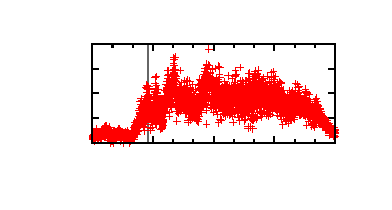
\includegraphics{/home/rik/workspace/ASL_student_project/Repositories/report-fork/Presentation/LaTeX_Template/images/windday}}%
    \gplfronttext
  \end{picture}%
\endgroup

	% GNUPLOT: LaTeX picture with Postscript
\begingroup
  \makeatletter
  \providecommand\color[2][]{%
    \GenericError{(gnuplot) \space\space\space\@spaces}{%
      Package color not loaded in conjunction with
      terminal option `colourtext'%
    }{See the gnuplot documentation for explanation.%
    }{Either use 'blacktext' in gnuplot or load the package
      color.sty in LaTeX.}%
    \renewcommand\color[2][]{}%
  }%
  \providecommand\includegraphics[2][]{%
    \GenericError{(gnuplot) \space\space\space\@spaces}{%
      Package graphicx or graphics not loaded%
    }{See the gnuplot documentation for explanation.%
    }{The gnuplot epslatex terminal needs graphicx.sty or graphics.sty.}%
    \renewcommand\includegraphics[2][]{}%
  }%
  \providecommand\rotatebox[2]{#2}%
  \@ifundefined{ifGPcolor}{%
    \newif\ifGPcolor
    \GPcolortrue
  }{}%
  \@ifundefined{ifGPblacktext}{%
    \newif\ifGPblacktext
    \GPblacktextfalse
  }{}%
  % define a \g@addto@macro without @ in the name:
  \let\gplgaddtomacro\g@addto@macro
  % define empty templates for all commands taking text:
  \gdef\gplbacktext{}%
  \gdef\gplfronttext{}%
  \makeatother
  \ifGPblacktext
    % no textcolor at all
    \def\colorrgb#1{}%
    \def\colorgray#1{}%
  \else
    % gray or color?
    \ifGPcolor
      \def\colorrgb#1{\color[rgb]{#1}}%
      \def\colorgray#1{\color[gray]{#1}}%
      \expandafter\def\csname LTw\endcsname{\color{white}}%
      \expandafter\def\csname LTb\endcsname{\color{black}}%
      \expandafter\def\csname LTa\endcsname{\color{black}}%
      \expandafter\def\csname LT0\endcsname{\color[rgb]{1,0,0}}%
      \expandafter\def\csname LT1\endcsname{\color[rgb]{0,1,0}}%
      \expandafter\def\csname LT2\endcsname{\color[rgb]{0,0,1}}%
      \expandafter\def\csname LT3\endcsname{\color[rgb]{1,0,1}}%
      \expandafter\def\csname LT4\endcsname{\color[rgb]{0,1,1}}%
      \expandafter\def\csname LT5\endcsname{\color[rgb]{1,1,0}}%
      \expandafter\def\csname LT6\endcsname{\color[rgb]{0,0,0}}%
      \expandafter\def\csname LT7\endcsname{\color[rgb]{1,0.3,0}}%
      \expandafter\def\csname LT8\endcsname{\color[rgb]{0.5,0.5,0.5}}%
    \else
      % gray
      \def\colorrgb#1{\color{black}}%
      \def\colorgray#1{\color[gray]{#1}}%
      \expandafter\def\csname LTw\endcsname{\color{white}}%
      \expandafter\def\csname LTb\endcsname{\color{black}}%
      \expandafter\def\csname LTa\endcsname{\color{black}}%
      \expandafter\def\csname LT0\endcsname{\color{black}}%
      \expandafter\def\csname LT1\endcsname{\color{black}}%
      \expandafter\def\csname LT2\endcsname{\color{black}}%
      \expandafter\def\csname LT3\endcsname{\color{black}}%
      \expandafter\def\csname LT4\endcsname{\color{black}}%
      \expandafter\def\csname LT5\endcsname{\color{black}}%
      \expandafter\def\csname LT6\endcsname{\color{black}}%
      \expandafter\def\csname LT7\endcsname{\color{black}}%
      \expandafter\def\csname LT8\endcsname{\color{black}}%
    \fi
  \fi
  \setlength{\unitlength}{0.0500bp}%
  \begin{picture}(3454.00,1700.00)%
    \gplgaddtomacro\gplbacktext{%
      \csname LTb\endcsname%
      \put(594,484){\makebox(0,0)[r]{\strut{} 0}}%
      \put(594,643){\makebox(0,0)[r]{\strut{} 2}}%
      \put(594,801){\makebox(0,0)[r]{\strut{} 4}}%
      \put(594,960){\makebox(0,0)[r]{\strut{} 6}}%
      \put(594,1118){\makebox(0,0)[r]{\strut{} 8}}%
      \put(594,1277){\makebox(0,0)[r]{\strut{} 10}}%
      \put(594,1435){\makebox(0,0)[r]{\strut{} 12}}%
      \put(726,264){\makebox(0,0){\strut{}30}}%
      \put(1503,264){\makebox(0,0){\strut{}31}}%
      \put(2280,264){\makebox(0,0){\strut{}32}}%
      \put(3057,264){\makebox(0,0){\strut{}33}}%
      \put(1891,154){\makebox(0,0){\strut{}time $[\si{\minute}]$}}%
    }%
    \gplgaddtomacro\gplfronttext{%
    }%
    \gplbacktext
    \put(0,0){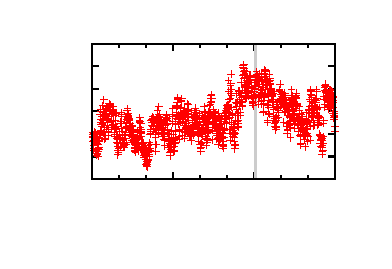
\includegraphics{/home/rik/workspace/ASL_student_project/Repositories/report-fork/Presentation/LaTeX_Template/images/windminute}}%
    \gplfronttext
  \end{picture}%
\endgroup

	\tiny{Wind speed observations in $[\si{\metre\per\second}$], \cite{www:googleheliostat}} 
	}
%    \def\figurewidth{{0.5\textwidth}}
%    \def\figureheight{0.6\figurewidth}
\end{minipage}

\clearpage
\ETHslide
\section*{System Overview}
%\addcontentsline{toc}{section}{Control Approach}
\vspace*{\fill}

\begin{figure}[h]
\centering
\scalebox{1}{
%\begin{tikzpicture}[auto, font=\small]
% coordinates
\coordinate (orig) at (0,0);
\coordinate (in1) at (0,-0.75);
\coordinate (in2) at (0,-1.75);
\coordinate (out1) at (12,-1.75/2);
\coordinate (LLA) at (1.5,-1.5);
\coordinate (LLB) at (4,-2.5);
\coordinate (LLC) at (6.5,-1.75);
\coordinate (LLD) at (9,-1.75);
\coordinate (in2inter1) at (1.5,-1.75);
\coordinate (out1inter1) at (11.5,-1.75/2);
\coordinate (out1inter2) at (3,-2.75);


% nodes
\node[draw, minimum width=1.5cm, minimum height=1.5cm, anchor=south west, text width=1.5cm, align=center] (A) at (LLA) {Position\\Control};
\node[draw, minimum width=1.5cm, minimum height=2cm, anchor=south west, text width=1.5cm, align=center] (B) at (LLB) {Attitude\\Control};
\node[draw, minimum width=1.5cm, minimum height=1.75cm, anchor=south west, text width=1.5cm, align=center] (C) at (LLC) {Allocation\\Map};
\node[draw, minimum width=1.5cm, minimum height=1.75cm, anchor=south west, text width=1.5cm, align=center] (D) at (LLD) {MAV\\Dynamics};

% edges
\draw[->] (in1) -- node[above] {$\mathbf{r}_{ref},\mathbf{v}_{ref}$} (A.180);

\draw[->] ($(A.0) + (0,0.5)$) -- node[above] {$T_{ref}$} ($(C.180) + (0,1.25/2)$);
\draw[->] (A.0) -- node[above] {$\phi_{ref}$} ($(B.180) + (0,0.75)$);
\draw[->] ($(A.0) - (0,0.5)$) -- node[above] {$\theta_{ref}$} ($(B.180) + (0,0.25)$);

\draw[-] (in2) -- node[above] {$\psi_{ref}$} (in2inter1);
\draw[->] (in2inter1) -- node {} ($(B.180) -  (0,0.25)$);

\draw[->] (B.0) -- node[above] {$\boldsymbol{\tau}_{ref}$} ($(C.180) - (0,1.25/2)$);

\draw[->] (C.0) -- node[above] {$\mathbf{n}_{ref}$} (D.180);

\draw[-] (D.0) -- node[] {} (out1inter1);
\path[fill] (out1inter1) circle[radius=1pt];
\draw[->] (out1inter1) -- node[] {} (out1);

\path[draw,-] (out1inter1) |- node[near end,below] {$\mathbf{r},\mathbf{v},\mathbf{q},\boldsymbol{\omega}$} (out1inter2) ;
\path[draw,->] (out1inter2) |- ($(B.180) - (0,0.75)$) ;
\path[draw,->] (out1inter2) -| ($(A.270)$) ;

%  %coordinates
%  \coordinate (orig)   at (0,0);
%  \coordinate (LLD)    at (4,0);
%  \coordinate (AroneA) at (-1/2,11/2);
%  \coordinate (ArtwoA) at (-1/2,5);
%  \coordinate (ArthrA) at (-1/2,9/2);
%  \coordinate (LLA)    at (1,4);
%  \coordinate (LLB)    at (4,4);
%  \coordinate (LLC)    at (7,4);
%  \coordinate (AroneC) at (25/2,11/2);
%  \coordinate (ArtwoC) at (25/2,5);
%  \coordinate (ArthrC) at (25/2,9/2);
%  \coordinate (conCBD) at (21/2,9/2);
%  \coordinate (conCB)  at (21/2,7/2);
%  \coordinate (coCBD)  at (11,5);
%  \coordinate (coCB)   at (11,3);
%  \coordinate (conCBA) at (23/2,11/2);
%  \coordinate (conCA)  at (23/2,5/2);
%%
%%  %nodes
%  \node[draw, minimum width=2cm, minimum height=2cm, anchor=south west, text width=2cm, align=center] (A) at (LLA) {Impedance\\control};
%  \node[draw, minimum width=2cm, minimum height=2cm, anchor=south west, text width=2cm, align=center] (B) at (LLB) {Inverse\\Dynamics};
%  \node[draw, minimum width=3cm, minimum height=2cm, anchor=south west, text width=2cm, align=center] (C) at (LLC) {Manipulator\\and\\environment};
%  \node[draw, minimum width=2cm, minimum height=2cm, anchor=south west, text width=2cm, align=center] (D) at (LLD) {Direct\\kinematics};
%
%  %edges
%  \draw[->] (AroneA) -- node[above]{$p_d, R_d$} ($(A.180) + (0,1/2)$);
%  \draw[->] (ArtwoA) -- node[above]{$v_d$} (A.180);
%  \draw[->] (ArthrA) -- node[above]{$v_d$} ($(A.180) + (0,-1/2)$);
%
%  \draw[->] (A.0) -- node[above] {$\alpha$} (B.180);
%  \draw[->] (B.0) -- node[above] {$\tau$} (C.180);
%
%  \draw[->] ($(C.0) + (0,1/2)$) -- node[above, pos=0.2]{$h_e$} (AroneC);
%  \draw[->] (C.0) -- node[above, pos=0.2]{$q$} (ArtwoC);
%  \draw[->] ($(C.0) + (0,-1/2)$) -- node[above, pos=0.2]{$q$} (ArthrC);
%
%  \path[fill] (conCBD) circle[radius=1pt] (conCB) circle[radius=1pt];
%  \path[draw,->] (conCBD) -- (conCB) -| ($(B.270) + (1/2,0)$);
%
%  \path[fill] (coCBD) circle[radius=1pt] (coCB) circle[radius=1pt];
%  \path[draw,->] (coCBD)  -- (coCB) -| (B.270);
%
%  \path[fill] (conCBA) circle[radius=1pt] (conCA) circle[radius=1pt];
%  \path[draw,->] (conCBA) -- (conCA) -| ($(B.270) + (-1/2,0)$);
%
%  \path[draw,->] (conCB) |- ($(D.0) + (0,1/2)$);
%  \path[draw,->] (coCB)  |- ($(D.0) + (0,-1/2)$);
%
%  \path[draw,->] (conCA) |- ($(A.270) + (-1/2,0) + (0,-9/2)$) -- ($(A.270) + (-1/2,0)$);
%
%  \path[draw,->] ($(D.180) + (0,1/2)$)  -| node[above,pos=0.2] {$p_e,r_e$} ($(A.270) + (1/2,0)$);
%  \path[draw,->] ($(D.180) + (0,-1/2)$) -| node[above,pos=0.15] {$v_e$} (A.270);

\end{tikzpicture}

\begin{tikzpicture}[auto, font=\small]
% coordinates
\coordinate (orig) at (0,0);
\coordinate (LLA) at (2,0);
\coordinate (LLB) at (5.5,0);
\coordinate (outinter) at (8,0);
\coordinate (out) at (9,0);


% nodes
\node[draw, minimum width=1.5cm, minimum height=1.5cm, anchor=west, text width=1.5cm, align=center] (A) at (LLA) {Position\\Control};
\node[draw, minimum width=1.5cm, minimum height=1.5cm, anchor=west, text width=1.5cm, align=center,fill=black,opacity=0.6] (B) at (LLB) {MAV \\Black Box};

% edges
\draw[->] (orig) -- node[above] {$\mathbf{r}_{ref},\mathbf{v}_{ref},\psi_{ref}$} (A.180);
\draw[->] (A.0) -- node[above] {$\begin{bmatrix}
T_{ref} \\ \phi_{ref} \\ \theta_{ref} \\ \psi_{ref}
\end{bmatrix}$} (B.180);
\draw[->] (B.0) -- (out);
\coordinate (feedback) at ($(A.270)-(0,0.75)$);
\draw[-] (outinter) |- node[above,near end] {$\mathbf{r},\mathbf{v},\mathbf{q},\boldsymbol{\omega},\mathbf{w}$} (feedback);
\draw[->] (feedback) -- (A.270);

\end{tikzpicture}

}
\end{figure}
\begin{itemize}
\item[\ETHitem] Cascaded control
\item[\ETHitem] Given attitude control
\item[\ETHitem] Given state and wind estimation
\item[\ETHitem] SysId attitude and thrust dynamics
\end{itemize}

\vspace*{\fill}
\clearpage
\ETHslide
\section*{Control System}
%\addcontentsline{toc}{section}{Control System}
\vspace*{\fill}
\begin{figure}[h]
\centering
\scalebox{0.5}{
\begin{tikzpicture}[auto, font=\small]
% coordinates
\coordinate (orig) at (0,0);
% inputs
\coordinate (Tin) at (orig);
\coordinate (phiin) at ($(orig)- (0,1.75)$);
\coordinate (thetain) at ($(phiin)- (0,1.75)$);
\coordinate (psiin) at ($(thetain)- (0,1.75)$);
% boxes
\coordinate (LLA) at ($(Tin) + (0.75,-0.75)$);
\coordinate (LLB) at ($(phiin) + (0.75,-0.75)$);
\coordinate (LLC) at ($(thetain) + (0.75,-0.75)$);
\coordinate (LLD) at ($(LLC) + (1.5+1.25,0)$);

% nodes
% boxes
\node[draw,minimum width=1.5cm, minimum height=1.5cm, anchor=south west, text width=1.5cm, align=center] (A) at (LLA) {$\Large 1$};
\node[draw,minimum width=1.5cm, minimum height=1.5cm, anchor=south west, text width=1.5cm, align=center] (B) at (LLB) {$2$nd Order};
\node[draw,minimum width=1.5cm, minimum height=1.5cm, anchor=south west, text width=1.5cm, align=center] (C) at (LLC) {$2$nd Order};
\node[draw,minimum width=3cm, minimum height=3.25cm, anchor=south west, align=center] (D) at (LLD) {Newton\\
Law};

\node[draw,minimum width=0.75cm, minimum height=0.75cm, anchor=west, text width=0.75cm, align=center] (E) at ($(D.0) + (0.5,0)$) {$\Large \int$};
\node[draw,minimum width=0.75cm, minimum height=0.75cm, anchor=west, text width=0.75cm, align=center] (F) at ($(E.0) + (0.5,0)$) {$\Large \int$};
% coordinates at boxes
\coordinate (DTin) at ($(D.180) + (0,2*0.55)$);
\coordinate (Dphiin) at ($(D.180) + (0,1*0.55)$);
\coordinate (Dthetain) at ($(D.180)$);
\coordinate (Dpsiin) at ($(D.180) - (0,1*0.55)$);
\coordinate (Ddxin) at ($(D.180) - (0,2*0.55)$);
\coordinate[above=of D.90] (win);
%lines
\draw[->] (Tin) -- node[at start,above]{$T_{ref}$} (A.180);
\draw[->] (phiin) -- node[at start,above]{$\phi_{ref}$} (B.180);
\draw[->] (thetain) -- node[at start,above]{$\theta_{ref}$} (C.180);
\draw[->] (A.0) -| node[near start,above]{$T$} ($(DTin) - (0.5,0)$) -- (DTin);
\draw[->] (B.0) -| node[near start,above]{$\phi$} ($(Dphiin) - (0.5,0)$) --  (Dphiin);
\draw[->] (C.0) -| node[near start,above]{$\theta$} ($(Dthetain) - (0.75,0)$) -- (Dthetain);
\draw[->] (psiin) -| node[at start,above]{$\psi_{m}$} ($(Dpsiin) - (0.5,0)$) -- (Dpsiin);

\draw[->] (D.0) -- node[above]{${\mathbf{a}}$} (E.180);
\draw[->] (E.0) -- node[above]{${\mathbf{v}}$} (F.180);
\coordinate (out) at ($(F.0) + (0.5,0)$);
\draw[->] (F.0) -- node[above]{$\mathbf{r}$} (out);

\draw[->] ($(E.0) + (0.5/2,0)$) |- ($(D.south west) - (0.25,0.5)$) |- (Ddxin);

\draw[->] (win) node[above]{$\E[\mathbf{w}]$}  -- (D.90);


\end{tikzpicture}

}
\end{figure}
\tiny{
\begin{align}
f\left(\mathbf{x},\mathbf{u},\mathbf{w}\right) &= \ddt \mathbf{x}  
= \begin{bmatrix}
\mathbf{A}_\phi \begin{bmatrix}
\frac{1}{8}\dot{\phi} \\ \phi
\end{bmatrix}
+ \mathbf{B}_\phi \phi_{ref} \\
\mathbf{A}_\theta \begin{bmatrix}
\frac{1}{8}\dot{\theta} \\ \theta
\end{bmatrix}
+ \mathbf{B}_\theta \theta_{ref} \\
\mathbf{v}\\
\frac{1}{m} \left( \mathbf{F}_{T,total} + \mathbf{F}_{D,total} \right)  + \begin{bmatrix}
0 \\ 0 \\ -g
\end{bmatrix} 
\end{bmatrix} \nonumber
\end{align}
}
\normalsize{}

%\begin{minipage}{0.6\textwidth}
%\end{minipage}
%\begin{minipage}{0.39\textwidth}
%\end{minipage}

\vspace*{\fill}
\clearpage
\addcontentsline{toc}{section}{Control}
\ETHslide
\section*{Receding Horizon Control}
%\addcontentsline{toc}{section}{}
\vspace*{\fill}

\begin{figure}[h]
\centering
\scalebox{0.6}{
\begin{tikzpicture}[auto, font=\small]
% coordinates
\coordinate (orig) at (0,0);
\coordinate (LLA) at (orig);
\coordinate (LLB) at (6.5,0);
\coordinate (out) at (12.5,0);


% nodes
\node[draw, minimum width=5cm, minimum height = 4cm, anchor=west, text width=5cm,align=center] (A) at (LLA) {\begin{align*}
&\argmin_{U_t}&  &\sum_{k=0}^{N-1} q(x_{t+k},u_{t+k}) \\
&\text{s.t.}  &  &x_t = x(t) \\
&	          &  &x_{t+k+1} = Ax_{t+k} + Bu_{t+k} \\
&	          &  &x_{t+k}\in\mathcal{X}, \; u_{t+k}\in\mathcal{U}
\end{align*}};
\node[draw, minimum width=4cm, minimum height = 4cm, anchor=west, text width=4cm,align=center] (B) at (LLB) {\Huge{\text{Plant}}};

% edges
\draw[->] (A.0) -- node[above] {$u^*_t$} (B.180);
\draw[->] (B.0) -- node[above] {Output $y(t)$} (out);
\coordinate (stateinter) at ($(A.270) - (0,1)$);
\draw[-] (B.270) |- node[near end, above] {State $x(t)$} (stateinter);
\draw[->] (stateinter) -- (A.270);


% edges
%\draw[->] (in1) -- node[above] {$\mathbf{r}_{ref},\mathbf{v}_{ref}$} (A.180);
%
%\draw[->] ($(A.0) + (0,0.5)$) -- node[above] {$T_{ref}$} ($(C.180) + (0,1.25/2)$);
%\draw[->] (A.0) -- node[above] {$\phi_{ref}$} ($(B.180) + (0,0.75)$);
%\draw[->] ($(A.0) - (0,0.5)$) -- node[above] {$\theta_{ref}$} ($(B.180) + (0,0.25)$);
%
%\draw[-] (in2) -- node[above] {$\psi_{ref}$} (in2inter1);
%\draw[->] (in2inter1) -- node {} ($(B.180) -  (0,0.25)$);
%
%\draw[->] (B.0) -- node[above] {$\boldsymbol{\tau}_{ref}$} ($(C.180) - (0,1.25/2)$);
%
%\draw[->] (C.0) -- node[above] {$\mathbf{n}_{ref}$} (D.180);
%
%\draw[-] (D.0) -- node[] {} (out1inter1);
%\path[fill] (out1inter1) circle[radius=1pt];
%\draw[->] (out1inter1) -- node[] {} (out1);
%
%\path[draw,-] (out1inter1) |- node[near end,below] {$\mathbf{x},\mathbf{\dot{x}},\mathbf{q},\boldsymbol{\omega}$} (out1inter2) ;
%\path[draw,->] (out1inter2) |- ($(B.180) - (0,0.75)$) ;
%\path[draw,->] (out1inter2) -| ($(A.270)$) ;

\end{tikzpicture}
}
\end{figure} 
At each sample time:
\begin{itemize}
\item[\ETHitem] Measure/estimate current state $x(t)$
\item[\ETHitem] Find the optimal input sequence for the entire planning window $N$: $U_t^* = \{ u_t^*, u_{t+1}^*, \ldots, u_{t+N-1}^* \}$
\item[\ETHitem] Implement the first control action $u_t^*$
\end{itemize}

\vspace*{\fill}
\clearpage
\ETHslide
\section*{Receding Horizon Control}
%\addcontentsline{toc}{section}{}
\vspace*{\fill}

Advantages:
\begin{itemize}
\item[\ETHitem] Input and output constraints
\item[\ETHitem] Predictive
\item[\ETHitem] Intuitive
\end{itemize}
Disadvantages:
\begin{itemize}
\item[\ETHitem] No robustness guarantees
\item[\ETHitem] OCP computationally expensive
\end{itemize}

\vspace*{\fill}
\clearpage
\ETHslide
\section*{Linear and nonlinear MPC}
\vspace*{\fill}

\begin{itemize}
\item[\ETHitem] deterministic wind feed-forward
\item[\ETHitem] offset-free constant reference tracking
\item[\ETHitem] trajectory tracking
\end{itemize}

Difference:
\begin{itemize}
\item[\ETHitem] MPC linearization about hovering
\item[\ETHitem] NMPC nonlinear dynamics
\end{itemize}

\vspace*{\fill}
\clearpage
%\ETHslide
\section*{Linear MPC}
%\addcontentsline{toc}{section}{}
\vspace*{\fill}

\begin{itemize}
\item[\ETHitem] \underline{Linearization}: About hovering
\item[\ETHitem] \underline{Offset-free}: System augmented with constant input disturbance 
\item[\ETHitem] \underline{Constant Disturbances}: Estimated with Luenberger observer
\item[\ETHitem] \underline{Reference tracking}: Tracking all $N$ future reference positions and velocities (feed-forward)
\item[\ETHitem] \underline{Input constraints}: Limited thrust, roll and pitch
\item[\ETHitem] \underline{Terminal penalty $P$}: Solution of algebraic Riccati equation
\item[\ETHitem] \underline{CVXGEN}: Generate hard-coded convex optimization solver
\end{itemize}

\vspace*{\fill}
\clearpage
%\ETHslide
\section*{Linear MPC OCP}
%\addcontentsline{toc}{section}{}
\footnotesize{
\begin{align}
&\min_{u(\cdot),x(\cdot)}
& & ||x_N-\bar{x}_t||_P^2 + \sum_{k=0}^{N-1} ||x_k - \bar{x}_t||_Q^2 + ||u_k - \bar{u}_t||_R^2  \nonumber\\
& \text{s.t.} 
& & x_{k+1} = A x_k + B u_k + B_w w_k + B_d d_k, & k = 0, \ldots, N-1 \nonumber\\
& & & w_{k+1} = w_k  & k = 0, \ldots, N-1 \nonumber\\
& & & d_{k+1} = d_k, & k = 0, \ldots, N-1 \nonumber\\
& & & \begin{bmatrix}
T_{min} \\ -30\si{\degree} \\ -30\si{\degree}
\end{bmatrix} \leq u_k \leq \begin{bmatrix}
T_{max} \\ 30\si{\degree} \\ 30\si{\degree}
\end{bmatrix} & k = 0, \ldots, N-1 \nonumber\\
& & & x_0 = \hat x (t), \; d_0 = \hat d(t), \; w_0 = \hat w(t) \nonumber \\
& & & N=40 \nonumber
\end{align}
}
\normalsize{}
\clearpage
%\ETHslide
\section*{Linear MPC Algorithm}
%\addcontentsline{toc}{section}{}
\vspace*{\fill}

At every sample time:
\begin{itemize}
\item[\ETHitem] Update state $\hat{x}(t)$ and disturbance $\hat{d}(t)$ estimation
\item[\ETHitem] Calculate $N+1$ desired steady-state inputs $\bar{u}_t$ and states $\bar{x}_t$
\item[\ETHitem] Solve finite-horizon optimal control problem (CVXGEN)
\item[\ETHitem] Apply first optimal control action to system
\end{itemize}

\vspace*{\fill}
\clearpage
%\ETHslide
\section*{Nonlinear MPC}
%\addcontentsline{toc}{section}{}
\vspace*{\fill}
No stability guarantees, no optimality guarantees
\begin{itemize}
\item[\ETHitem] \underline{Offset-free}: System augmented with integrator
\item[\ETHitem] \underline{Reference tracking}: Tracking all $N$ future reference positions and velocities (feed-forward)
\item[\ETHitem] \underline{Input constraints}: Limited thrust, roll and pitch
\item[\ETHitem] \underline{Terminal penalty P}: Solution of algebraic Riccati equation of linearized system
\item[\ETHitem] \underline{ACADO}: Generate hard-coded nonlinear optimization solver
\item[\ETHitem] \underline{qpDUNES}: Interior point method/active set for solving sparse OCP
\end{itemize}

\vspace*{\fill}
\clearpage
\addcontentsline{toc}{section}{Simulation}
\ETHslide
\section*{Nonlinear MPC OCP}
%\addcontentsline{toc}{section}{}
\vspace*{\fill}
\footnotesize{
\begin{align}
&\min_{x(\cdot),u(\cdot)} &&\int_{t}^{t+NT_s} \left( ||x(\tau)-x_{ref}(\tau)||_Q^2 + ||u(\tau)-u_{ref}(\tau)||_R^2 \d \tau \right)  \nonumber \\
&&&+ ||x(t+NT_s)-x_{ref}(t+NT_s)||_P^2 \nonumber \\
&s.t. &&\dot{x}(\tau) = f(x(\tau),u(\tau),w(\tau),\psi(\tau)) \nonumber \\
&&&\dot{w}(\tau) = 0 \nonumber \\
&&&\dot{\psi}(\tau) = 0 \nonumber \\
&&&\begin{bmatrix}
T_{min} \\ -45 \si{\degree} \\-45 \si{\degree}
\end{bmatrix} \leq u(\tau) \leq \begin{bmatrix}
T_{max} \\ 45 \si{\degree} \\45 \si{\degree}
\end{bmatrix} , \quad \forall\tau\in\left[t,t+NT_s\right] \nonumber \\
&&&x(t) = \hat{x}(t),\; w(t) = \hat{w}(t), \; \psi(t) = \hat{\psi}(t)  \nonumber \\
&&&N=100\nonumber
\end{align}
}
\normalsize{}
\vspace*{\fill}
\clearpage
%\ETHslide
\section*{Nonlinear MPC Algorithm}
%\addcontentsline{toc}{section}{}
\vspace*{\fill}

At every sample time:
\begin{itemize}
\item[\ETHitem] Set current state, wind and heading
\item[\ETHitem] Set $N+1$ references
\item[\ETHitem] Set previous optimal solution as warm start
\item[\ETHitem] Solve finite-horizon optimal control problem (ACADO)
\item[\ETHitem] Update integrator
\item[\ETHitem] Apply first optimal control action to system
\end{itemize}

\vspace*{\fill}
\clearpage
%\ETHslide
\section*{Step Response: Linear MPC}
%\addcontentsline{toc}{section}{}
\vspace*{\fill}

\begin{minipage}{0.5\textwidth}
	\centering
	\tiny{
	% This file was created by matlab2tikz.
% Minimal pgfplots version: 1.3
%
\definecolor{mycolor1}{rgb}{0.00000,0.44700,0.74100}%
\definecolor{mycolor2}{rgb}{0.85000,0.32500,0.09800}%
\definecolor{mycolor3}{rgb}{0.92900,0.69400,0.12500}%
%
\begin{tikzpicture}

\begin{axis}[%
width=\figurewidth,
height=0.984009\figureheight,
at={(0\figurewidth,0\figureheight)},
scale only axis,
xmin=0,
xmax=5,
xlabel={time $[\si{\second}]$},
ymin=-0.2,
ymax=1.2,
ylabel={position $[\si{\metre}]$},
axis x line*=bottom,
axis y line*=left,
legend style={at={(0.5,1.03)},anchor=south,legend columns=3,legend cell align=left,align=left,draw=white!15!black}
]
\addplot [color=mycolor1,solid]
  table[row sep=crcr]{%
0	0\\
0.01	1.14690425758758e-08\\
0.02	3.9139247376254e-07\\
0.03	2.83493392441896e-06\\
0.04	1.11051834900563e-05\\
0.05	3.12788497901201e-05\\
0.06	7.18257334289189e-05\\
0.07	0.000143559484600181\\
0.08	0.000259428712558198\\
0.09	0.000434230940921711\\
0.1	0.000684297077484614\\
0.11	0.00102717519265354\\
0.12	0.00148133123930672\\
0.13	0.00206587644600224\\
0.14	0.00280032594689838\\
0.15	0.00370439000250268\\
0.16	0.0047977972180332\\
0.17	0.00610014799051753\\
0.18	0.00763079651509766\\
0.19	0.00940876480511783\\
0.2	0.0114526846522818\\
0.21	0.0137807407968232\\
0.22	0.0164106284954103\\
0.23	0.0193595249032115\\
0.24	0.0226440708237129\\
0.25	0.0262803601235094\\
0.26	0.0302839346288481\\
0.27	0.0346698148326636\\
0.28	0.0394526012157968\\
0.29	0.044646482601358\\
0.3	0.0502656879782431\\
0.31	0.0563257286016026\\
0.32	0.0628426614025463\\
0.33	0.0698305493531942\\
0.34	0.0773002587755007\\
0.35	0.0852591459937297\\
0.36	0.0937110624737891\\
0.37	0.10265645737235\\
0.38	0.112092670157311\\
0.39	0.122014712549827\\
0.4	0.132415897683296\\
0.41	0.143287379804692\\
0.42	0.154617504758948\\
0.43	0.166391506536651\\
0.44	0.178591430063641\\
0.45	0.191196207501871\\
0.46	0.204181846842149\\
0.47	0.217521705701489\\
0.48	0.231186839716325\\
0.49	0.245146401191358\\
0.5	0.259368025637102\\
0.51	0.273818231820918\\
0.52	0.288462828823561\\
0.53	0.303267317616087\\
0.54	0.318197276391322\\
0.55	0.333218720529993\\
0.56	0.348298429762913\\
0.57	0.363404236834843\\
0.58	0.37850527376272\\
0.59	0.393572173563614\\
0.6	0.408577227045264\\
0.61	0.423494495838767\\
0.62	0.438299884244244\\
0.63	0.452971173597493\\
0.64	0.467488023671323\\
0.65	0.481831943133623\\
0.66	0.495986218252608\\
0.67	0.509935817073701\\
0.68	0.523667306773268\\
0.69	0.537168771172672\\
0.7	0.550429646962763\\
0.71	0.563440613862694\\
0.72	0.576193589079729\\
0.73	0.58868171088866\\
0.74	0.6008992960234\\
0.75	0.612841777357085\\
0.76	0.624505646924077\\
0.77	0.635888407683714\\
0.78	0.646988518112545\\
0.79	0.657805330684049\\
0.8	0.668339026920506\\
0.81	0.678590550676979\\
0.82	0.688561540863623\\
0.83	0.698254264592939\\
0.84	0.707671551606085\\
0.85	0.716816730725328\\
0.86	0.725693568974922\\
0.87	0.734306213903445\\
0.88	0.742659139527276\\
0.89	0.750757096200328\\
0.9	0.758605064603075\\
0.91	0.766208213937729\\
0.92	0.773571864319226\\
0.93	0.7807014532656\\
0.94	0.787602506118118\\
0.95	0.79428061016196\\
0.96	0.800741392172575\\
0.97	0.806990499080787\\
0.98	0.813033580514812\\
0.99	0.818876272806302\\
1	0.824524185901435\\
1.01	0.829982894661978\\
1.02	0.835257931695948\\
1.03	0.840354781017045\\
1.04	0.845278872297848\\
1.05	0.850035575522238\\
1.06	0.854630196208461\\
1.07	0.859067970746821\\
1.08	0.863354061992374\\
1.09	0.867493555060194\\
1.1	0.871491453182171\\
1.11	0.87535267357497\\
1.12	0.879082043435866\\
1.13	0.882684296044236\\
1.14	0.886164066941702\\
1.15	0.889525890212335\\
1.16	0.892774194894376\\
1.17	0.895913301554866\\
1.18	0.89894741902765\\
1.19	0.901880641396319\\
1.2	0.904716945274591\\
1.21	0.907460187348123\\
1.22	0.910114102235678\\
1.23	0.912682300757355\\
1.24	0.915168268599074\\
1.25	0.917575365368301\\
1.26	0.91990682406119\\
1.27	0.922165750954413\\
1.28	0.924355125928457\\
1.29	0.926477803223071\\
1.3	0.928536512619652\\
1.31	0.930533861039892\\
1.32	0.932472334512499\\
1.33	0.934354300260928\\
1.34	0.936182009135477\\
1.35	0.937957598820566\\
1.36	0.939683097826402\\
1.37	0.941360429681311\\
1.38	0.942991417158007\\
1.39	0.944577786539642\\
1.4	0.946121171929167\\
1.41	0.94762311958439\\
1.42	0.949085092253852\\
1.43	0.95050847348715\\
1.44	0.951894571894401\\
1.45	0.953244625331588\\
1.46	0.954559804967361\\
1.47	0.955841219192675\\
1.48	0.957089917465828\\
1.49	0.95830689408983\\
1.5	0.959493091809487\\
1.51	0.960649405225339\\
1.52	0.961776684031765\\
1.53	0.962875736081455\\
1.54	0.963947330277348\\
1.55	0.964992199293578\\
1.56	0.966011042127964\\
1.57	0.967004526489633\\
1.58	0.967973291026402\\
1.59	0.968917947397434\\
1.6	0.969839082197384\\
1.61	0.970737258738867\\
1.62	0.971613018700483\\
1.63	0.972466883647928\\
1.64	0.97329935643587\\
1.65	0.974110922498328\\
1.66	0.974902051034955\\
1.67	0.975673196093077\\
1.68	0.976424797558711\\
1.69	0.977157282068922\\
1.7	0.977871063849827\\
1.71	0.978566545483366\\
1.72	0.979244118610003\\
1.73	0.979904164573894\\
1.74	0.980547055017221\\
1.75	0.981173152429806\\
1.76	0.981782810659678\\
1.77	0.982376375387689\\
1.78	0.982954184569631\\
1.79	0.983516568848525\\
1.8	0.984063851939205\\
1.81	0.98459635098693\\
1.82	0.985114376901473\\
1.83	0.985618234667903\\
1.84	0.986108223635136\\
1.85	0.986584637783194\\
1.86	0.987047765970034\\
1.87	0.987497892158757\\
1.88	0.987935295625965\\
1.89	0.988360251152017\\
1.9	0.988773029193527\\
1.91	0.989173896039905\\
1.92	0.989563113954603\\
1.93	0.989940941301279\\
1.94	0.990307632655264\\
1.95	0.990663438902003\\
1.96	0.991008607323251\\
1.97	0.991343381671389\\
1.98	0.991668002232454\\
1.99	0.991982705879022\\
2	0.992287726114213\\
2.01	0.992583293107279\\
2.02	0.992869633721411\\
2.03	0.993146971534488\\
2.04	0.993415526853936\\
2.05	0.993675516726601\\
2.06	0.993927154944095\\
2.07	0.994170652044259\\
2.08	0.994406215309351\\
2.09	0.994634048761547\\
2.1	0.994854353156842\\
2.11	0.995067325977704\\
2.12	0.995273161424908\\
2.13	0.995472050409008\\
2.14	0.995664180541957\\
2.15	0.995849736129257\\
2.16	0.996028898162972\\
2.17	0.996201844315918\\
2.18	0.99636874893754\\
2.19	0.996529783051571\\
2.2	0.996685114355665\\
2.21	0.996834907223171\\
2.22	0.996979322707083\\
2.23	0.997118518546175\\
2.24	0.997252649173727\\
2.25	0.997381865729044\\
2.26	0.99750631607147\\
2.27	0.997626144796828\\
2.28	0.997741493256335\\
2.29	0.997852499577948\\
2.3	0.997959298690065\\
2.31	0.998062022347525\\
2.32	0.998160799159841\\
2.33	0.998255754621606\\
2.34	0.998347011144909\\
2.35	0.998434688093666\\
2.36	0.998518901819783\\
2.37	0.998599765701016\\
2.38	0.998677390180386\\
2.39	0.998751882807035\\
2.4	0.998823348278413\\
2.41	0.998891888483678\\
2.42	0.998957602548179\\
2.43	0.999020586878969\\
2.44	0.999080935211246\\
2.45	0.999138738655606\\
2.46	0.999194085746011\\
2.47	0.999247062488347\\
2.48	0.999297752409465\\
2.49	0.999346236606577\\
2.5	0.999392593796917\\
2.51	0.999436900367539\\
2.52	0.999479230425164\\
2.53	0.999519655845981\\
2.54	0.999558246325312\\
2.55	0.999595069427053\\
2.56	0.999630190632842\\
2.57	0.999663673390859\\
2.58	0.999695579164216\\
2.59	0.99972596747887\\
2.6	0.999754895971014\\
2.61	0.999782420433913\\
2.62	0.999808594864135\\
2.63	0.999833471507161\\
2.64	0.999857100902338\\
2.65	0.999879531927163\\
2.66	0.999900811840885\\
2.67	0.999920986327398\\
2.68	0.999940099537431\\
2.69	0.999958194130019\\
2.7	0.999975311313261\\
2.71	0.999991490884347\\
2.72	1.00000677126887\\
2.73	1.0000211895594\\
2.74	1.00003478155337\\
2.75	1.00004758179019\\
2.76	1.00005962358774\\
2.77	1.00007093907802\\
2.78	1.00008155924222\\
2.79	1.00009151394502\\
2.8	1.00010083196819\\
2.81	1.0001095410435\\
2.82	1.0001176678849\\
2.83	1.00012523822003\\
2.84	1.00013227682103\\
2.85	1.00013880753467\\
2.86	1.00014485331174\\
2.87	1.00015043623588\\
2.88	1.00015557755159\\
2.89	1.00016029769167\\
2.9	1.00016461630395\\
2.91	1.00016855227737\\
2.92	1.00017212376735\\
2.93	1.00017534822059\\
2.94	1.00017824239919\\
2.95	1.00018082240403\\
2.96	1.00018310369766\\
2.97	1.00018510112642\\
2.98	1.00018682894197\\
2.99	1.00018830082224\\
3	1.0001895298917\\
3.01	1.00019052874104\\
3.02	1.00019130944627\\
3.03	1.00019188358723\\
3.04	1.00019226226551\\
3.05	1.00019245612184\\
3.06	1.00019247535289\\
3.07	1.00019232972757\\
3.08	1.00019202860275\\
3.09	1.00019158093855\\
3.1	1.00019099531308\\
3.11	1.00019027993667\\
3.12	1.00018944266568\\
3.13	1.00018849101585\\
3.14	1.00018743217512\\
3.15	1.00018627301615\\
3.16	1.00018502010826\\
3.17	1.00018367972914\\
3.18	1.00018225787599\\
3.19	1.00018076027637\\
3.2	1.00017919239868\\
3.21	1.00017755946223\\
3.22	1.00017586644697\\
3.23	1.00017411810293\\
3.24	1.00017231895925\\
3.25	1.00017047333292\\
3.26	1.00016858533726\\
3.27	1.00016665889001\\
3.28	1.00016469772118\\
3.29	1.00016270538063\\
3.3	1.00016068524532\\
3.31	1.00015864052636\\
3.32	1.00015657427575\\
3.33	1.00015448939287\\
3.34	1.00015238863081\\
3.35	1.00015027460233\\
3.36	1.00014814978574\\
3.37	1.00014601653043\\
3.38	1.00014387706228\\
3.39	1.00014173348882\\
3.4	1.00013958780423\\
3.41	1.00013744189408\\
3.42	1.00013529753998\\
3.43	1.00013315642394\\
3.44	1.00013102013269\\
3.45	1.00012889016172\\
3.46	1.00012676791919\\
3.47	1.00012465472973\\
3.48	1.00012255183804\\
3.49	1.00012046041239\\
3.5	1.00011838154793\\
3.51	1.00011631626989\\
3.52	1.00011426553669\\
3.53	1.00011223024288\\
3.54	1.00011021122194\\
3.55	1.00010820924908\\
3.56	1.00010622504376\\
3.57	1.00010425927227\\
3.58	1.00010231255009\\
3.59	1.00010038544424\\
3.6	1.00009847847545\\
3.61	1.00009659212034\\
3.62	1.00009472681339\\
3.63	1.00009288294898\\
3.64	1.0000910608832\\
3.65	1.00008926093571\\
3.66	1.0000874833914\\
3.67	1.00008572850213\\
3.68	1.00008399648828\\
3.69	1.00008228754026\\
3.7	1.00008060182002\\
3.71	1.00007893946243\\
3.72	1.00007730057664\\
3.73	1.00007568524737\\
3.74	1.00007409353615\\
3.75	1.00007252548251\\
3.76	1.00007098110515\\
3.77	1.00006946040299\\
3.78	1.00006796335626\\
3.79	1.00006648992748\\
3.8	1.00006504006245\\
3.81	1.00006361369118\\
3.82	1.00006221072874\\
3.83	1.00006083107616\\
3.84	1.00005947462122\\
3.85	1.00005814123923\\
3.86	1.0000568307938\\
3.87	1.00005554313753\\
3.88	1.00005427811274\\
3.89	1.00005303555208\\
3.9	1.00005181527921\\
3.91	1.00005061710935\\
3.92	1.00004944084993\\
3.93	1.00004828630106\\
3.94	1.00004715325615\\
3.95	1.00004604150233\\
3.96	1.00004495082101\\
3.97	1.0000438809883\\
3.98	1.00004283177547\\
3.99	1.00004180294935\\
4	1.0000407942728\\
4.01	1.00003980550501\\
4.02	1.00003883640193\\
4.03	1.00003788671663\\
4.04	1.00003695619958\\
4.05	1.00003604459902\\
4.06	1.00003515166127\\
4.07	1.00003427713099\\
4.08	1.00003342075149\\
4.09	1.00003258226496\\
4.1	1.00003176141278\\
4.11	1.00003095793569\\
4.12	1.00003017157409\\
4.13	1.00002940206821\\
4.14	1.00002864915832\\
4.15	1.00002791258496\\
4.16	1.0000271920891\\
4.17	1.00002648741231\\
4.18	1.00002579829695\\
4.19	1.00002512448633\\
4.2	1.00002446572482\\
4.21	1.00002382175805\\
4.22	1.000023192333\\
4.23	1.00002257719815\\
4.24	1.00002197610358\\
4.25	1.0000213888011\\
4.26	1.00002081504434\\
4.27	1.00002025458886\\
4.28	1.00001970719224\\
4.29	1.00001917261417\\
4.3	1.0000186506165\\
4.31	1.00001814096336\\
4.32	1.0000176434212\\
4.33	1.00001715775887\\
4.34	1.00001668374765\\
4.35	1.00001622116135\\
4.36	1.00001576977633\\
4.37	1.00001532937152\\
4.38	1.00001489972855\\
4.39	1.00001448063167\\
4.4	1.00001407186787\\
4.41	1.00001367322689\\
4.42	1.00001328450122\\
4.43	1.00001290548614\\
4.44	1.00001253597976\\
4.45	1.00001217578299\\
4.46	1.0000118246996\\
4.47	1.00001148253619\\
4.48	1.00001114910224\\
4.49	1.00001082421007\\
4.5	1.00001050767488\\
4.51	1.00001019931473\\
4.52	1.00000989895055\\
4.53	1.00000960640612\\
4.54	1.00000932150808\\
4.55	1.00000904408591\\
4.56	1.00000877397194\\
4.57	1.0000085110013\\
4.58	1.00000825501196\\
4.59	1.00000800584467\\
4.6	1.00000776334297\\
4.61	1.00000752735314\\
4.62	1.00000729772424\\
4.63	1.00000707430803\\
4.64	1.00000685695898\\
4.65	1.00000664553424\\
4.66	1.00000643989363\\
4.67	1.00000623989958\\
4.68	1.00000604541716\\
4.69	1.000005856314\\
4.7	1.0000056724603\\
4.71	1.00000549372877\\
4.72	1.00000531999465\\
4.73	1.00000515113563\\
4.74	1.00000498703186\\
4.75	1.00000482756589\\
4.76	1.00000467262267\\
4.77	1.00000452208949\\
4.78	1.00000437585598\\
4.79	1.00000423381406\\
4.8	1.00000409585789\\
4.81	1.00000396188389\\
4.82	1.00000383179066\\
4.83	1.00000370547897\\
4.84	1.00000358285174\\
4.85	1.00000346381396\\
4.86	1.00000334827273\\
4.87	1.00000323613716\\
4.88	1.00000312731837\\
4.89	1.00000302172947\\
4.9	1.0000029192855\\
4.91	1.00000281990341\\
4.92	1.00000272350202\\
4.93	1.00000263000202\\
4.94	1.0000025393259\\
4.95	1.00000245139792\\
4.96	1.00000236614411\\
4.97	1.00000228349221\\
4.98	1.00000220337166\\
4.99	1.00000212571355\\
5	1.00000205045059\\
};
\addlegendentry{x};

\addplot [color=mycolor2,solid]
  table[row sep=crcr]{%
0	0\\
0.01	-1.55177660043528e-23\\
0.02	-2.67274574431345e-13\\
0.03	-8.98478263104176e-12\\
0.04	-6.16971360850354e-11\\
0.05	-2.2297262599863e-10\\
0.06	-5.63143026467177e-10\\
0.07	-1.12284298361237e-09\\
0.08	-1.88432511755817e-09\\
0.09	-2.76567687508838e-09\\
0.1	-3.64552946441174e-09\\
0.11	-4.41845777422109e-09\\
0.12	-5.07566267856705e-09\\
0.13	-5.8022177532598e-09\\
0.14	-7.08094738967342e-09\\
0.15	-9.79335376595711e-09\\
0.16	-1.53093607479971e-08\\
0.17	-2.55595124262953e-08\\
0.18	-4.30855042456767e-08\\
0.19	-7.10706674426555e-08\\
0.2	-1.13348156435952e-07\\
0.21	-1.74371887537051e-07\\
0.22	-2.59154892994293e-07\\
0.23	-3.73184505633744e-07\\
0.24	-5.22321304450265e-07\\
0.25	-7.12687183644643e-07\\
0.26	-9.50546848844114e-07\\
0.27	-1.24219077730769e-06\\
0.28	-1.59382668232799e-06\\
0.29	-2.01145696563217e-06\\
0.3	-2.50083839741196e-06\\
0.31	-3.06760240797529e-06\\
0.32	-3.71707167725793e-06\\
0.33	-4.45375845931693e-06\\
0.34	-5.28110164802155e-06\\
0.35	-6.2013868806401e-06\\
0.36	-7.21574575886128e-06\\
0.37	-8.32418173750178e-06\\
0.38	-9.52562808564532e-06\\
0.39	-1.08180840114527e-05\\
0.4	-1.21986976671083e-05\\
0.41	-1.36636215405781e-05\\
0.42	-1.52078212511313e-05\\
0.43	-1.68249449506927e-05\\
0.44	-1.85072365635161e-05\\
0.45	-2.02454859514349e-05\\
0.46	-2.20290156011993e-05\\
0.47	-2.38457057545927e-05\\
0.48	-2.56820535053694e-05\\
0.49	-2.7523249500673e-05\\
0.5	-2.93532879262815e-05\\
0.51	-3.11551278793805e-05\\
0.52	-3.29109039961258e-05\\
0.53	-3.46021804032711e-05\\
0.54	-3.62102398147108e-05\\
0.55	-3.77163976172807e-05\\
0.56	-3.91023293216542e-05\\
0.57	-4.03503989586696e-05\\
0.58	-4.14439759662762e-05\\
0.59	-4.23677288447864e-05\\
0.6	-4.31078852893436e-05\\
0.61	-4.36524505040723e-05\\
0.62	-4.39913777799745e-05\\
0.63	-4.41166879710807e-05\\
0.64	-4.4022536979539e-05\\
0.65	-4.37052284723403e-05\\
0.66	-4.31631549803496e-05\\
0.67	-4.23966926793223e-05\\
0.68	-4.14080953210245e-05\\
0.69	-4.0201372108246e-05\\
0.7	-3.87820764274962e-05\\
0.71	-3.71571458276573e-05\\
0.72	-3.53348196710979e-05\\
0.73	-3.33245214406003e-05\\
0.74	-3.11367042307167e-05\\
0.75	-2.87826571303649e-05\\
0.76	-2.62742808490266e-05\\
0.77	-2.36238982191234e-05\\
0.78	-2.08441046481987e-05\\
0.79	-1.79476467740375e-05\\
0.8	-1.49473233722516e-05\\
0.81	-1.18559048272061e-05\\
0.82	-8.68606847721948e-06\\
0.83	-5.45034752712645e-06\\
0.84	-2.16109133746943e-06\\
0.85	1.16956506379163e-06\\
0.86	4.52972435129838e-06\\
0.87	7.90774515517454e-06\\
0.88	1.12922570310589e-05\\
0.89	1.46721737566446e-05\\
0.9	1.80367062948586e-05\\
0.91	2.13753764675059e-05\\
0.92	2.46780320774217e-05\\
0.93	2.79348639181285e-05\\
0.94	3.1136424831428e-05\\
0.95	3.42736507260171e-05\\
0.96	3.73378832616531e-05\\
0.97	4.03208937381183e-05\\
0.98	4.32149071241458e-05\\
0.99	4.6012623559986e-05\\
1	4.87072356379909e-05\\
1.01	5.12924464175047e-05\\
1.02	5.37624883358501e-05\\
1.03	5.61121417726326e-05\\
1.04	5.83367522237249e-05\\
1.05	6.04322451668551e-05\\
1.06	6.23951380584343e-05\\
1.07	6.42225485817213e-05\\
1.08	6.59121988746599e-05\\
1.09	6.74624153915347e-05\\
1.1	6.88721241051929e-05\\
1.11	7.01408410084991e-05\\
1.12	7.12686582696756e-05\\
1.13	7.22562261213009e-05\\
1.14	7.31047306430977e-05\\
1.15	7.38158678396493e-05\\
1.16	7.43918144833401e-05\\
1.17	7.48351962291226e-05\\
1.18	7.51490535247034e-05\\
1.19	7.53368061328633e-05\\
1.2	7.54022166466045e-05\\
1.21	7.53493532080872e-05\\
1.22	7.5182552206618e-05\\
1.23	7.4906381388617e-05\\
1.24	7.4525603458809e-05\\
1.25	7.40451405260746e-05\\
1.26	7.34700397571762e-05\\
1.27	7.28054405400056e-05\\
1.28	7.20565433986139e-05\\
1.29	7.1228580845552e-05\\
1.3	7.03267903036216e-05\\
1.31	6.93563891796637e-05\\
1.32	6.83225520828487e-05\\
1.33	6.7230389812676e-05\\
1.34	6.60849302353201e-05\\
1.35	6.4891101489701e-05\\
1.36	6.36537177967103e-05\\
1.37	6.23774673860227e-05\\
1.38	6.10669022910793e-05\\
1.39	5.97264297678983e-05\\
1.4	5.83603051437719e-05\\
1.41	5.6972625921854e-05\\
1.42	5.55673269881557e-05\\
1.43	5.41481767878571e-05\\
1.44	5.27187743576218e-05\\
1.45	5.12825471193545e-05\\
1.46	4.98427493470689e-05\\
1.47	4.84024610270873e-05\\
1.48	4.69645869285745e-05\\
1.49	4.55318566267065e-05\\
1.5	4.41068255154299e-05\\
1.51	4.26918765155732e-05\\
1.52	4.12892223072781e-05\\
1.53	3.99009079919933e-05\\
1.54	3.85288141298157e-05\\
1.55	3.71746601195017e-05\\
1.56	3.5840007899629e-05\\
1.57	3.45262659547071e-05\\
1.58	3.32346936119513e-05\\
1.59	3.19664056143293e-05\\
1.6	3.07223769541826e-05\\
1.61	2.95034479497437e-05\\
1.62	2.83103295445746e-05\\
1.63	2.71436088075918e-05\\
1.64	2.60037546091094e-05\\
1.65	2.48911234463552e-05\\
1.66	2.38059653931056e-05\\
1.67	2.27484301849698e-05\\
1.68	2.17185734599793e-05\\
1.69	2.07163630983891e-05\\
1.7	1.97416855572434e-05\\
1.71	1.87943520874167e-05\\
1.72	1.78741047813834e-05\\
1.73	1.69806224715827e-05\\
1.74	1.61135264717885e-05\\
1.75	1.52723861629456e-05\\
1.76	1.44567243984517e-05\\
1.77	1.36660227272053e-05\\
1.78	1.2899726430771e-05\\
1.79	1.21572493674795e-05\\
1.8	1.14379786149317e-05\\
1.81	1.07412789023046e-05\\
1.82	1.0066496824586e-05\\
1.83	9.41296483206426e-06\\
1.84	8.78000498987775e-06\\
1.85	8.16693250406011e-06\\
1.86	7.57305901219492e-06\\
1.87	6.99769563846176e-06\\
1.88	6.44015581445848e-06\\
1.89	5.89975786869395e-06\\
1.9	5.37582738856945e-06\\
1.91	4.86769935109936e-06\\
1.92	4.37472003714186e-06\\
1.93	3.89624874729581e-06\\
1.94	3.4316593232627e-06\\
1.95	2.98034147077236e-06\\
1.96	2.54170189942064e-06\\
1.97	2.11516530153398e-06\\
1.98	1.70017517513649e-06\\
1.99	1.29619449278496e-06\\
2	9.02706229819881e-07\\
2.01	5.19213764313915e-07\\
2.02	1.45241155793293e-07\\
2.03	-2.19666690220209e-07\\
2.04	-5.75943965946514e-07\\
2.05	-9.2400400107407e-07\\
2.06	-1.26423938855455e-06\\
2.07	-1.59702218942254e-06\\
2.08	-1.92270420948325e-06\\
2.09	-2.24161734138587e-06\\
2.1	-2.55407396622661e-06\\
2.11	-2.86036740523562e-06\\
2.12	-3.16077241489888e-06\\
2.13	-3.45554572025588e-06\\
2.14	-3.74492658120674e-06\\
2.15	-4.02913738682897e-06\\
2.16	-4.30838427287259e-06\\
2.17	-4.58285775784168e-06\\
2.18	-4.85273339365374e-06\\
2.19	-5.11817242701403e-06\\
2.2	-5.37932246797859e-06\\
2.21	-5.63631816242578e-06\\
2.22	-5.8892818634403e-06\\
2.23	-6.13832424752011e-06\\
2.24	-6.38354480538523e-06\\
2.25	-6.62503234190936e-06\\
2.26	-6.86286554612671e-06\\
2.27	-7.09711361420269e-06\\
2.28	-7.32783690773088e-06\\
2.29	-7.55508763322548e-06\\
2.3	-7.77891053063549e-06\\
2.31	-7.99934356016813e-06\\
2.32	-8.21641857828746e-06\\
2.33	-8.43016199601746e-06\\
2.34	-8.64059541383743e-06\\
2.35	-8.84773622833281e-06\\
2.36	-9.05159820730264e-06\\
2.37	-9.25219203072844e-06\\
2.38	-9.44952579578951e-06\\
2.39	-9.64360548588338e-06\\
2.4	-9.83443540332788e-06\\
2.41	-1.00220185652061e-05\\
2.42	-1.0206357063212e-05\\
2.43	-1.03874523889031e-05\\
2.44	-1.05653057260969e-05\\
2.45	-1.07399182123916e-05\\
2.46	-1.09112911719551e-05\\
2.47	-1.10794263218111e-05\\
2.48	-1.12443259538738e-05\\
2.49	-1.14059930949471e-05\\
2.5	-1.15644316468209e-05\\
2.51	-1.1719646508478e-05\\
2.52	-1.18716436822729e-05\\
2.53	-1.20204303657979e-05\\
2.54	-1.21660150317739e-05\\
2.55	-1.23084074983775e-05\\
2.56	-1.24476189893757e-05\\
2.57	-1.2583662183573e-05\\
2.58	-1.2716551254502e-05\\
2.59	-1.28463019013803e-05\\
2.6	-1.29729313721322e-05\\
2.61	-1.30964584790982e-05\\
2.62	-1.32169036079202e-05\\
2.63	-1.33342887199873e-05\\
2.64	-1.34486373487479e-05\\
2.65	-1.35599745901338e-05\\
2.66	-1.36683270873077e-05\\
2.67	-1.37737230099164e-05\\
2.68	-1.38761920280273e-05\\
2.69	-1.39757652809215e-05\\
2.7	-1.40724753409316e-05\\
2.71	-1.41663561725243e-05\\
2.72	-1.42574430868524e-05\\
2.73	-1.43457726920399e-05\\
2.74	-1.44313828399759e-05\\
2.75	-1.45143125712532e-05\\
2.76	-1.45946020582054e-05\\
2.77	-1.46722925438251e-05\\
2.78	-1.47474262763385e-05\\
2.79	-1.48200464401775e-05\\
2.8	-1.4890197084103e-05\\
2.81	-1.49579230471496e-05\\
2.82	-1.50232698830046e-05\\
2.83	-1.50862837834242e-05\\
2.84	-1.51470115020437e-05\\
2.85	-1.52055002806108e-05\\
2.86	-1.52617977767292e-05\\
2.87	-1.53159519906252e-05\\
2.88	-1.53680111913439e-05\\
2.89	-1.54180238432944e-05\\
2.9	-1.54660385358293e-05\\
2.91	-1.55121039165619e-05\\
2.92	-1.5556268625604e-05\\
2.93	-1.55985812299898e-05\\
2.94	-1.56390901588894e-05\\
2.95	-1.56778436402219e-05\\
2.96	-1.57148896391633e-05\\
2.97	-1.57502757989466e-05\\
2.98	-1.57840493842686e-05\\
2.99	-1.58162572275421e-05\\
3	-1.58469456781656e-05\\
3.01	-1.58761605549255e-05\\
3.02	-1.59039471015898e-05\\
3.03	-1.59303499457115e-05\\
3.04	-1.59554130606162e-05\\
3.05	-1.59791797305175e-05\\
3.06	-1.60016925186785e-05\\
3.07	-1.60229932385117e-05\\
3.08	-1.60431229275009e-05\\
3.09	-1.60621218238103e-05\\
3.1	-1.60800293454458e-05\\
3.11	-1.6096884071828e-05\\
3.12	-1.61127237276371e-05\\
3.13	-1.61275851687959e-05\\
3.14	-1.61415043704596e-05\\
3.15	-1.61545164168914e-05\\
3.16	-1.61666554931101e-05\\
3.17	-1.61779548782059e-05\\
3.18	-1.61884469402279e-05\\
3.19	-1.61981631325596e-05\\
3.2	-1.62071339917057e-05\\
3.21	-1.62153891364204e-05\\
3.22	-1.62229572681181e-05\\
3.23	-1.62298661725111e-05\\
3.24	-1.62361427224257e-05\\
3.25	-1.62418128817523e-05\\
3.26	-1.62469017104883e-05\\
3.27	-1.62514333708342e-05\\
3.28	-1.62554311343067e-05\\
3.29	-1.62589173898309e-05\\
3.3	-1.62619136527754e-05\\
3.31	-1.62644405748913e-05\\
3.32	-1.62665179551185e-05\\
3.33	-1.62681647512171e-05\\
3.34	-1.62693990921819e-05\\
3.35	-1.62702382913981e-05\\
3.36	-1.62706988604909e-05\\
3.37	-1.62707965238219e-05\\
3.38	-1.62705462335852e-05\\
3.39	-1.62699621854519e-05\\
3.4	-1.62690578347124e-05\\
3.41	-1.62678459128664e-05\\
3.42	-1.6266338444608e-05\\
3.43	-1.62645467651545e-05\\
3.44	-1.62624815378694e-05\\
3.45	-1.62601527721276e-05\\
3.46	-1.62575698413762e-05\\
3.47	-1.62547415013422e-05\\
3.48	-1.62516759083421e-05\\
3.49	-1.62483806376496e-05\\
3.5	-1.62448627018805e-05\\
3.51	-1.62411285693558e-05\\
3.52	-1.6237184182405e-05\\
3.53	-1.62330349755774e-05\\
3.54	-1.62286858937284e-05\\
3.55	-1.62241414099521e-05\\
3.56	-1.62194055433329e-05\\
3.57	-1.62144818764929e-05\\
3.58	-1.62093735729122e-05\\
3.59	-1.62040833940021e-05\\
3.6	-1.6198613715915e-05\\
3.61	-1.6192966546073e-05\\
3.62	-1.61871435394038e-05\\
3.63	-1.61811460142699e-05\\
3.64	-1.6174974968081e-05\\
3.65	-1.61686310925817e-05\\
3.66	-1.61621147888049e-05\\
3.67	-1.61554261816856e-05\\
3.68	-1.61485651343288e-05\\
3.69	-1.61415312619285e-05\\
3.7	-1.6134323945332e-05\\
3.71	-1.61269423442492e-05\\
3.72	-1.6119385410103e-05\\
3.73	-1.61116518985209e-05\\
3.74	-1.61037403814665e-05\\
3.75	-1.60956492590109e-05\\
3.76	-1.60873767707448e-05\\
3.77	-1.60789210068325e-05\\
3.78	-1.60702799187087e-05\\
3.79	-1.60614513294205e-05\\
3.8	-1.60524329436175e-05\\
3.81	-1.60432223571921e-05\\
3.82	-1.60338170665739e-05\\
3.83	-1.60242144776813e-05\\
3.84	-1.60144119145356e-05\\
3.85	-1.60044066275399e-05\\
3.86	-1.59941958014306e-05\\
3.87	-1.5983776562903e-05\\
3.88	-1.59731459879208e-05\\
3.89	-1.59623011087101e-05\\
3.9	-1.59512389204495e-05\\
3.91	-1.59399563876575e-05\\
3.92	-1.59284504502873e-05\\
3.93	-1.59167180295344e-05\\
3.94	-1.59047560333632e-05\\
3.95	-1.58925613617614e-05\\
3.96	-1.58801309117278e-05\\
3.97	-1.58674615820021e-05\\
3.98	-1.58545502775432e-05\\
3.99	-1.58413939137642e-05\\
4	-1.58279894205312e-05\\
4.01	-1.58143337459333e-05\\
4.02	-1.5800423859833e-05\\
4.03	-1.57862567572014e-05\\
4.04	-1.57718294612493e-05\\
4.05	-1.57571390263587e-05\\
4.06	-1.57421825408245e-05\\
4.07	-1.57269571294116e-05\\
4.08	-1.57114599557357e-05\\
4.09	-1.56956882244755e-05\\
4.1	-1.56796391834219e-05\\
4.11	-1.56633101253711e-05\\
4.12	-1.56466983898701e-05\\
4.13	-1.56298013648189e-05\\
4.14	-1.5612616487937e-05\\
4.15	-1.55951412481001e-05\\
4.16	-1.55773731865533e-05\\
4.17	-1.55593098980064e-05\\
4.18	-1.55409490316167e-05\\
4.19	-1.55222882918661e-05\\
4.2	-1.55033254393367e-05\\
4.21	-1.54840582913899e-05\\
4.22	-1.54644847227556e-05\\
4.23	-1.54446026660347e-05\\
4.24	-1.54244101121209e-05\\
4.25	-1.54039051105451e-05\\
4.26	-1.53830857697479e-05\\
4.27	-1.53619502572839e-05\\
4.28	-1.53404967999621e-05\\
4.29	-1.53187236839254e-05\\
4.3	-1.5296629254675e-05\\
4.31	-1.52742119170406e-05\\
4.32	-1.52514701351021e-05\\
4.33	-1.52284024320655e-05\\
4.34	-1.52050073900946e-05\\
4.35	-1.51812836501046e-05\\
4.36	-1.51572299115174e-05\\
4.37	-1.51328449319831e-05\\
4.38	-1.51081275270703e-05\\
4.39	-1.50830765699269e-05\\
4.4	-1.50576909909139e-05\\
4.41	-1.50319697772157e-05\\
4.42	-1.50059119724268e-05\\
4.43	-1.49795166761196e-05\\
4.44	-1.49527830433924e-05\\
4.45	-1.49257102844018e-05\\
4.46	-1.48982976638799e-05\\
4.47	-1.48705445006381e-05\\
4.48	-1.48424501670592e-05\\
4.49	-1.48140140885791e-05\\
4.5	-1.47852357431595e-05\\
4.51	-1.47561146607526e-05\\
4.52	-1.47266504227594e-05\\
4.53	-1.46968426614825e-05\\
4.54	-1.46666910595737e-05\\
4.55	-1.46361953494782e-05\\
4.56	-1.46053553128768e-05\\
4.57	-1.45741707801247e-05\\
4.58	-1.45426416296901e-05\\
4.59	-1.45107677875918e-05\\
4.6	-1.44785492268365e-05\\
4.61	-1.44459859668574e-05\\
4.62	-1.44130780729532e-05\\
4.63	-1.4379825655729e-05\\
4.64	-1.4346228870539e-05\\
4.65	-1.43122879169319e-05\\
4.66	-1.42780030380984e-05\\
4.67	-1.4243374520322e-05\\
4.68	-1.42084026924336e-05\\
4.69	-1.41730879252683e-05\\
4.7	-1.41374306311273e-05\\
4.71	-1.41014312632427e-05\\
4.72	-1.40650903152469e-05\\
4.73	-1.40284083206459e-05\\
4.74	-1.39913858522967e-05\\
4.75	-1.39540235218897e-05\\
4.76	-1.39163219794347e-05\\
4.77	-1.38782819127523e-05\\
4.78	-1.38399040469686e-05\\
4.79	-1.38011891440157e-05\\
4.8	-1.37621380021361e-05\\
4.81	-1.37227514553913e-05\\
4.82	-1.36830303731758e-05\\
4.83	-1.36429756597349e-05\\
4.84	-1.36025882536873e-05\\
4.85	-1.35618691275519e-05\\
4.86	-1.35208192872791e-05\\
4.87	-1.34794397717863e-05\\
4.88	-1.34377316524924e-05\\
4.89	-1.33956960328401e-05\\
4.9	-1.33533340478023e-05\\
4.91	-1.33106468633852e-05\\
4.92	-1.32676356761337e-05\\
4.93	-1.32243017126485e-05\\
4.94	-1.3180646229116e-05\\
4.95	-1.31366705108495e-05\\
4.96	-1.30923758718358e-05\\
4.97	-1.30477636542908e-05\\
4.98	-1.30028352282288e-05\\
4.99	-1.29575919910504e-05\\
5	-1.29120353671474e-05\\
};
\addlegendentry{y};

\addplot [color=mycolor3,solid]
  table[row sep=crcr]{%
0	0\\
0.01	6.31662727401026e-06\\
0.02	3.91018142696076e-05\\
0.03	0.000104209148433768\\
0.04	0.000194748950631202\\
0.05	0.000301515048542168\\
0.06	0.000420073764218748\\
0.07	0.000549818686110807\\
0.08	0.0006908598001473\\
0.09	0.000842684990761694\\
0.1	0.0010037235556633\\
0.11	0.00117129149928856\\
0.12	0.00134169735225791\\
0.13	0.00151040872988545\\
0.14	0.00167223486621253\\
0.15	0.0018215060068518\\
0.16	0.00195224221555152\\
0.17	0.00205830914249662\\
0.18	0.00213356341564744\\
0.19	0.00217200996079291\\
0.2	0.00216796022628764\\
0.21	0.00211610806835239\\
0.22	0.00201159568440498\\
0.23	0.0018500758109816\\
0.24	0.00162776552079048\\
0.25	0.00134148988728493\\
0.26	0.000988715070369732\\
0.27	0.000567645493320515\\
0.28	7.74557345557011e-05\\
0.29	-0.000481726760471964\\
0.3	-0.0011079258882694\\
0.31	-0.00179480371248079\\
0.32	-0.00253302794387662\\
0.33	-0.00331461454358931\\
0.34	-0.00413410362686106\\
0.35	-0.00498798961511829\\
0.36	-0.00587376190759554\\
0.37	-0.00678904002927028\\
0.38	-0.00773061221296381\\
0.39	-0.00869272037142138\\
0.4	-0.0096657172943218\\
0.41	-0.0106369441802446\\
0.42	-0.0115921718335762\\
0.43	-0.0125165660292616\\
0.44	-0.0133953850833929\\
0.45	-0.0142145232066998\\
0.46	-0.0149609489546196\\
0.47	-0.0156230577564572\\
0.48	-0.0161909096166194\\
0.49	-0.0166563590703294\\
0.5	-0.0170132333143738\\
0.51	-0.0172574585786469\\
0.52	-0.0173871174891364\\
0.53	-0.0174024419323139\\
0.54	-0.0173057464545296\\
0.55	-0.0171013081845546\\
0.56	-0.0167952003030057\\
0.57	-0.0163950869883638\\
0.58	-0.0159099884246042\\
0.59	-0.0153500247983603\\
0.6	-0.0147261482213173\\
0.61	-0.0140498711886857\\
0.62	-0.0133329995471786\\
0.63	-0.0125873770317927\\
0.64	-0.0118246470943454\\
0.65	-0.0110560187376799\\
0.66	-0.0102919593953133\\
0.67	-0.00954191256879651\\
0.68	-0.00881418722239547\\
0.69	-0.00811589579357391\\
0.7	-0.00745258856603185\\
0.71	-0.00682817375618945\\
0.72	-0.0062452591701634\\
0.73	-0.00570541818261254\\
0.74	-0.00520934383926309\\
0.75	-0.00475693143782978\\
0.76	-0.00434738401917084\\
0.77	-0.00397935028235538\\
0.78	-0.00365103819924622\\
0.79	-0.0033603080040338\\
0.8	-0.00310475234321603\\
0.81	-0.00288176694056062\\
0.82	-0.00268861325899989\\
0.83	-0.00252247387312912\\
0.84	-0.00238050097586901\\
0.85	-0.0022598583591002\\
0.86	-0.00215775721093386\\
0.87	-0.00207148610764376\\
0.88	-0.00199843562080998\\
0.89	-0.00193611799762009\\
0.9	-0.00188218239858999\\
0.91	-0.00183442618967648\\
0.92	-0.00179080278440628\\
0.93	-0.00174942651715145\\
0.94	-0.00170857500284463\\
0.95	-0.00166668940360158\\
0.96	-0.00162237298149888\\
0.97	-0.00157438827175096\\
0.98	-0.00152164862845964\\
0.99	-0.00146320348985508\\
1	-0.00139822618250126\\
1.01	-0.00132601449358195\\
1.02	-0.00124599197189385\\
1.03	-0.00115770769687816\\
1.04	-0.0010608343044404\\
1.05	-0.000955164087528341\\
1.06	-0.000840605067521469\\
1.07	-0.000717175049917515\\
1.08	-0.000584995118477275\\
1.09	-0.000444282802020603\\
1.1	-0.000295344390265131\\
1.11	-0.000138566290872127\\
1.12	2.55935376780145e-05\\
1.13	0.000196614072420105\\
1.14	0.000373919794852111\\
1.15	0.000556889238689135\\
1.16	0.000744863387800075\\
1.17	0.00093715384105502\\
1.18	0.0011330509956677\\
1.19	0.00133183176693725\\
1.2	0.00153276658143975\\
1.21	0.00173512630425443\\
1.22	0.00193818882637527\\
1.23	0.00214124459521871\\
1.24	0.00234360139959142\\
1.25	0.00254458869924367\\
1.26	0.00274356147712183\\
1.27	0.0029399036073579\\
1.28	0.00313303074215588\\
1.29	0.00332239272782166\\
1.3	0.00350747556530011\\
1.31	0.00368780293437052\\
1.32	0.00386293786589185\\
1.33	0.00403248886365009\\
1.34	0.00419611722180642\\
1.35	0.00435353799418897\\
1.36	0.00450451239390528\\
1.37	0.00464884066257431\\
1.38	0.00478635747496876\\
1.39	0.00491692895806491\\
1.4	0.00504045048440244\\
1.41	0.00515684485832517\\
1.42	0.00526606071838358\\
1.43	0.00536807107059126\\
1.44	0.00546287190834862\\
1.45	0.00555048089377705\\
1.46	0.00563093677807332\\
1.47	0.00570430025267902\\
1.48	0.0057706531089262\\
1.49	0.00583009511503613\\
1.5	0.00588274158722215\\
1.51	0.0059287216090232\\
1.52	0.00596817656656433\\
1.53	0.00600125885221618\\
1.54	0.0060281306695211\\
1.55	0.0060489629076974\\
1.56	0.00606393407006067\\
1.57	0.00607322924827621\\
1.58	0.00607703913818662\\
1.59	0.00607555909506773\\
1.6	0.00606898822743073\\
1.61	0.00605752852929356\\
1.62	0.0060413840513663\\
1.63	0.00602076011192024\\
1.64	0.00599586254828555\\
1.65	0.00596689701004463\\
1.66	0.00593406830813735\\
1.67	0.00589758020008522\\
1.68	0.00585763523693675\\
1.69	0.0058144342583209\\
1.7	0.00576817561389046\\
1.71	0.00571905436634154\\
1.72	0.00566726154934086\\
1.73	0.00561298356400699\\
1.74	0.00555640172936353\\
1.75	0.0054976919581811\\
1.76	0.00543702448751226\\
1.77	0.0053745637021203\\
1.78	0.00531046802596835\\
1.79	0.0052448898657851\\
1.8	0.00517797559620022\\
1.81	0.00510986557885997\\
1.82	0.00504069420963453\\
1.83	0.00497058998912684\\
1.84	0.00489967561247409\\
1.85	0.00482806807503264\\
1.86	0.00475587879102279\\
1.87	0.00468321372261586\\
1.88	0.00461017351729242\\
1.89	0.00453685365199178\\
1.9	0.00446334461807527\\
1.91	0.00438973207477707\\
1.92	0.00431609698073635\\
1.93	0.00424251573667248\\
1.94	0.00416906036944208\\
1.95	0.00409579868963492\\
1.96	0.00402279442286226\\
1.97	0.00395010734509557\\
1.98	0.00387779344057514\\
1.99	0.0038059050622727\\
2	0.00373449105918534\\
2.01	0.00366359690250437\\
2.02	0.00359326481917638\\
2.03	0.00352353394335586\\
2.04	0.00345444045471012\\
2.05	0.00338601769346238\\
2.06	0.00331829627622615\\
2.07	0.00325130421401578\\
2.08	0.00318506703871868\\
2.09	0.00311960794741366\\
2.1	0.00305494790773449\\
2.11	0.00299110575207646\\
2.12	0.00292809827471677\\
2.13	0.00286594033002685\\
2.14	0.00280464492986955\\
2.15	0.00274422334019668\\
2.16	0.00268468518419358\\
2.17	0.00262603855213108\\
2.18	0.00256829007809323\\
2.19	0.00251144501198903\\
2.2	0.00245550729303148\\
2.21	0.00240047962515343\\
2.22	0.00234636357439731\\
2.23	0.00229315969582846\\
2.24	0.00224086762517362\\
2.25	0.00218948610401904\\
2.26	0.00213901300766272\\
2.27	0.00208944539419569\\
2.28	0.00204077954526871\\
2.29	0.00199301100049948\\
2.3	0.00194613459562429\\
2.31	0.00190014451380528\\
2.32	0.00185503433475837\\
2.33	0.0018107970705724\\
2.34	0.00176742520079995\\
2.35	0.00172491072308375\\
2.36	0.00168324519460726\\
2.37	0.00164241976235897\\
2.38	0.00160242519779421\\
2.39	0.00156325194043756\\
2.4	0.00152489012883752\\
2.41	0.00148732962341994\\
2.42	0.00145056003089719\\
2.43	0.00141457072929554\\
2.44	0.00137935089301915\\
2.45	0.00134488951757818\\
2.46	0.00131117544373445\\
2.47	0.00127819738089647\\
2.48	0.00124594392964614\\
2.49	0.00121440360331453\\
2.5	0.00118356484854863\\
2.51	0.00115341606482999\\
2.52	0.00112394562292122\\
2.53	0.00109514188240527\\
2.54	0.00106699320840975\\
2.55	0.00103948798686348\\
2.56	0.00101261463857975\\
2.57	0.000986361632052929\\
2.58	0.000960717495319002\\
2.59	0.000935670826894073\\
2.6	0.000911210305804049\\
2.61	0.000887324700731168\\
2.62	0.000864002878310455\\
2.63	0.00084123381061384\\
2.64	0.000819006581862509\\
2.65	0.000797310394409691\\
2.66	0.000776134574036869\\
2.67	0.000755468574606591\\
2.68	0.000735301982114727\\
2.69	0.000715624518184345\\
2.7	0.000696426043042357\\
2.71	0.000677696558018839\\
2.72	0.00065942620760744\\
2.73	0.000641605281232938\\
2.74	0.000624224214862716\\
2.75	0.000607273592292065\\
2.76	0.000590744145874492\\
2.77	0.000574626756588446\\
2.78	0.000558912453860665\\
2.79	0.000543592415274418\\
2.8	0.0005286579661512\\
2.81	0.000514100579003691\\
2.82	0.000499911872864747\\
2.83	0.000486083612694716\\
2.84	0.000472607708916699\\
2.85	0.000459476216890924\\
2.86	0.000446681335877764\\
2.87	0.000434215407384924\\
2.88	0.000422070913598897\\
2.89	0.000410240476426822\\
2.9	0.000398716856813055\\
2.91	0.00038749295336916\\
2.92	0.000376561800415871\\
2.93	0.000365916565958838\\
2.94	0.000355550549787473\\
2.95	0.000345457181655509\\
2.96	0.000335630019517544\\
2.97	0.000326062747805244\\
2.98	0.000316749175732515\\
2.99	0.000307683235622351\\
3	0.000298858981250217\\
3.01	0.000290270586200201\\
3.02	0.000281912342231099\\
3.03	0.000273778657650233\\
3.04	0.000265864055693286\\
3.05	0.000258163172908841\\
3.06	0.000250670757546594\\
3.07	0.000243381667948485\\
3.08	0.000236290870942226\\
3.09	0.000229393440236895\\
3.1	0.000222684554820442\\
3.11	0.000216159497359107\\
3.12	0.000209813652598903\\
3.13	0.000203642505769402\\
3.14	0.000197641640990211\\
3.15	0.000191806739680573\\
3.16	0.000186133578972616\\
3.17	0.000180618030128865\\
3.18	0.000175256056964622\\
3.19	0.000170043714275917\\
3.2	0.000164977146273725\\
3.21	0.00016005258502518\\
3.22	0.000155266348902525\\
3.23	0.000150614841040547\\
3.24	0.000146094547803222\\
3.25	0.000141702037260329\\
3.26	0.000137433957674717\\
3.27	0.000133287036000965\\
3.28	0.000129258076396082\\
3.29	0.00012534395874293\\
3.3	0.000121541637186972\\
3.31	0.000117848138686962\\
3.32	0.000114260561580121\\
3.33	0.000110776074162361\\
3.34	0.000107391913284019\\
3.35	0.000104105382961597\\
3.36	0.000100913853005917\\
3.37	9.78147576670951e-05\\
3.38	9.48055942966823e-05\\
3.39	9.18839220273101e-05\\
3.4	8.90473604701198e-05\\
3.41	8.62935884302416e-05\\
3.42	8.36203426405457e-05\\
3.43	8.10254165138586e-05\\
3.44	7.85066589138099e-05\\
3.45	7.60619729444435e-05\\
3.46	7.36893147587034e-05\\
3.47	7.13866923858702e-05\\
3.48	6.91521645780095e-05\\
3.49	6.69838396754581e-05\\
3.5	6.48798744913603e-05\\
3.51	6.283847321524e-05\\
3.52	6.08578863355746e-05\\
3.53	5.89364095813209e-05\\
3.54	5.70723828823218e-05\\
3.55	5.5264189348508e-05\\
3.56	5.35102542677892e-05\\
3.57	5.18090441225239e-05\\
3.58	5.01590656244329e-05\\
3.59	4.85588647678197e-05\\
3.6	4.70070259009395e-05\\
3.61	4.55021708153563e-05\\
3.62	4.40429578531141e-05\\
3.63	4.26280810315404e-05\\
3.64	4.12562691854938e-05\\
3.65	3.9926285126857e-05\\
3.66	3.86369248210747e-05\\
3.67	3.73870165805261e-05\\
3.68	3.6175420274521e-05\\
3.69	3.50010265556988e-05\\
3.7	3.38627561026121e-05\\
3.71	3.27595588782667e-05\\
3.72	3.16904134043934e-05\\
3.73	3.06543260512217e-05\\
3.74	2.9650330342521e-05\\
3.75	2.86774862756799e-05\\
3.76	2.77348796565856e-05\\
3.77	2.68216214490714e-05\\
3.78	2.59368471386942e-05\\
3.79	2.50797161106098e-05\\
3.8	2.42494110413075e-05\\
3.81	2.34451373039715e-05\\
3.82	2.26661223872324e-05\\
3.83	2.1911615327076e-05\\
3.84	2.11808861516784e-05\\
3.85	2.0473225338936e-05\\
3.86	1.97879432864584e-05\\
3.87	1.91243697937974e-05\\
3.88	1.8481853556687e-05\\
3.89	1.78597616730688e-05\\
3.9	1.72574791606787e-05\\
3.91	1.66744084859754e-05\\
3.92	1.61099691041932e-05\\
3.93	1.55635970103008e-05\\
3.94	1.50347443006544e-05\\
3.95	1.45228787451321e-05\\
3.96	1.40274833695406e-05\\
3.97	1.35480560480877e-05\\
3.98	1.30841091057179e-05\\
3.99	1.26351689301076e-05\\
4	1.22007755931227e-05\\
4.01	1.17804824815425e-05\\
4.02	1.13738559368562e-05\\
4.03	1.0980474903941e-05\\
4.04	1.05999305884335e-05\\
4.05	1.02318261226122e-05\\
4.06	9.87577623960685e-06\\
4.07	9.53140695575332e-06\\
4.08	9.19835526091784e-06\\
4.09	8.87626881662079e-06\\
4.1	8.5648056617849e-06\\
4.11	8.26363392593981e-06\\
4.12	7.97243154971791e-06\\
4.13	7.69088601248142e-06\\
4.14	7.4186940669157e-06\\
4.15	7.15556148043504e-06\\
4.16	6.90120278324564e-06\\
4.17	6.65534102291364e-06\\
4.18	6.41770752529038e-06\\
4.19	6.1880416616467e-06\\
4.2	5.96609062187349e-06\\
4.21	5.7516091936083e-06\\
4.22	5.54435954714901e-06\\
4.23	5.34411102601831e-06\\
4.24	5.15063994304664e-06\\
4.25	4.96372938184222e-06\\
4.26	4.78316900352026e-06\\
4.27	4.60875485856661e-06\\
4.28	4.4402892037127e-06\\
4.29	4.27758032370035e-06\\
4.3	4.12044235781898e-06\\
4.31	3.96869513109854e-06\\
4.32	3.82216399004589e-06\\
4.33	3.68067964281267e-06\\
4.34	3.54407800368667e-06\\
4.35	3.41220004179923e-06\\
4.36	3.28489163394499e-06\\
4.37	3.16200342141226e-06\\
4.38	3.04339067072365e-06\\
4.39	2.92891313818953e-06\\
4.4	2.81843493817754e-06\\
4.41	2.71182441500672e-06\\
4.42	2.60895401837344e-06\\
4.43	2.50970018221939e-06\\
4.44	2.41394320695448e-06\\
4.45	2.32156714494901e-06\\
4.46	2.23245968921328e-06\\
4.47	2.14651206517974e-06\\
4.48	2.0636189255099e-06\\
4.49	1.98367824784741e-06\\
4.5	1.90659123544025e-06\\
4.51	1.83226222055903e-06\\
4.52	1.76059857063783e-06\\
4.53	1.69151059706607e-06\\
4.54	1.62491146656178e-06\\
4.55	1.56071711506006e-06\\
4.56	1.49884616404797e-06\\
4.57	1.43921983928438e-06\\
4.58	1.38176189183824e-06\\
4.59	1.32639852138589e-06\\
4.6	1.27305830170645e-06\\
4.61	1.22167210831671e-06\\
4.62	1.17217304818871e-06\\
4.63	1.12449639149319e-06\\
4.64	1.07857950531423e-06\\
4.65	1.03436178928355e-06\\
4.66	9.9178461308162e-07\\
4.67	9.50791255753032e-07\\
4.68	9.11326846791804e-07\\
4.69	8.73338308943761e-07\\
4.7	8.36774302679047e-07\\
4.71	8.01585172292371e-07\\
4.72	7.67722893585647e-07\\
4.73	7.35141023084663e-07\\
4.74	7.03794648754227e-07\\
4.75	6.73640342166149e-07\\
4.76	6.44636112081319e-07\\
4.77	6.16741359406397e-07\\
4.78	5.89916833487017e-07\\
4.79	5.6412458969977e-07\\
4.8	5.39327948307042e-07\\
4.81	5.1549145453886e-07\\
4.82	4.92580839867791e-07\\
4.83	4.70562984443798e-07\\
4.84	4.49405880655121e-07\\
4.85	4.29078597784877e-07\\
4.86	4.09551247730586e-07\\
4.87	3.90794952829228e-07\\
4.88	3.72781816466621e-07\\
4.89	3.55484892146731e-07\\
4.9	3.38878151102383e-07\\
4.91	3.22936451501856e-07\\
4.92	3.07635508994304e-07\\
4.93	2.92951868423233e-07\\
4.94	2.78862877863112e-07\\
4.95	2.65346663793487e-07\\
4.96	2.52382104947474e-07\\
4.97	2.39948806699751e-07\\
4.98	2.28027076666055e-07\\
4.99	2.16597901339573e-07\\
5	2.05642923640811e-07\\
};
\addlegendentry{z};

\addplot [color=mycolor1,dashed,forget plot]
  table[row sep=crcr]{%
0	1\\
0.01	1\\
0.02	1\\
0.03	1\\
0.04	1\\
0.05	1\\
0.06	1\\
0.07	1\\
0.08	1\\
0.09	1\\
0.1	1\\
0.11	1\\
0.12	1\\
0.13	1\\
0.14	1\\
0.15	1\\
0.16	1\\
0.17	1\\
0.18	1\\
0.19	1\\
0.2	1\\
0.21	1\\
0.22	1\\
0.23	1\\
0.24	1\\
0.25	1\\
0.26	1\\
0.27	1\\
0.28	1\\
0.29	1\\
0.3	1\\
0.31	1\\
0.32	1\\
0.33	1\\
0.34	1\\
0.35	1\\
0.36	1\\
0.37	1\\
0.38	1\\
0.39	1\\
0.4	1\\
0.41	1\\
0.42	1\\
0.43	1\\
0.44	1\\
0.45	1\\
0.46	1\\
0.47	1\\
0.48	1\\
0.49	1\\
0.5	1\\
0.51	1\\
0.52	1\\
0.53	1\\
0.54	1\\
0.55	1\\
0.56	1\\
0.57	1\\
0.58	1\\
0.59	1\\
0.6	1\\
0.61	1\\
0.62	1\\
0.63	1\\
0.64	1\\
0.65	1\\
0.66	1\\
0.67	1\\
0.68	1\\
0.69	1\\
0.7	1\\
0.71	1\\
0.72	1\\
0.73	1\\
0.74	1\\
0.75	1\\
0.76	1\\
0.77	1\\
0.78	1\\
0.79	1\\
0.8	1\\
0.81	1\\
0.82	1\\
0.83	1\\
0.84	1\\
0.85	1\\
0.86	1\\
0.87	1\\
0.88	1\\
0.89	1\\
0.9	1\\
0.91	1\\
0.92	1\\
0.93	1\\
0.94	1\\
0.95	1\\
0.96	1\\
0.97	1\\
0.98	1\\
0.99	1\\
1	1\\
1.01	1\\
1.02	1\\
1.03	1\\
1.04	1\\
1.05	1\\
1.06	1\\
1.07	1\\
1.08	1\\
1.09	1\\
1.1	1\\
1.11	1\\
1.12	1\\
1.13	1\\
1.14	1\\
1.15	1\\
1.16	1\\
1.17	1\\
1.18	1\\
1.19	1\\
1.2	1\\
1.21	1\\
1.22	1\\
1.23	1\\
1.24	1\\
1.25	1\\
1.26	1\\
1.27	1\\
1.28	1\\
1.29	1\\
1.3	1\\
1.31	1\\
1.32	1\\
1.33	1\\
1.34	1\\
1.35	1\\
1.36	1\\
1.37	1\\
1.38	1\\
1.39	1\\
1.4	1\\
1.41	1\\
1.42	1\\
1.43	1\\
1.44	1\\
1.45	1\\
1.46	1\\
1.47	1\\
1.48	1\\
1.49	1\\
1.5	1\\
1.51	1\\
1.52	1\\
1.53	1\\
1.54	1\\
1.55	1\\
1.56	1\\
1.57	1\\
1.58	1\\
1.59	1\\
1.6	1\\
1.61	1\\
1.62	1\\
1.63	1\\
1.64	1\\
1.65	1\\
1.66	1\\
1.67	1\\
1.68	1\\
1.69	1\\
1.7	1\\
1.71	1\\
1.72	1\\
1.73	1\\
1.74	1\\
1.75	1\\
1.76	1\\
1.77	1\\
1.78	1\\
1.79	1\\
1.8	1\\
1.81	1\\
1.82	1\\
1.83	1\\
1.84	1\\
1.85	1\\
1.86	1\\
1.87	1\\
1.88	1\\
1.89	1\\
1.9	1\\
1.91	1\\
1.92	1\\
1.93	1\\
1.94	1\\
1.95	1\\
1.96	1\\
1.97	1\\
1.98	1\\
1.99	1\\
2	1\\
2.01	1\\
2.02	1\\
2.03	1\\
2.04	1\\
2.05	1\\
2.06	1\\
2.07	1\\
2.08	1\\
2.09	1\\
2.1	1\\
2.11	1\\
2.12	1\\
2.13	1\\
2.14	1\\
2.15	1\\
2.16	1\\
2.17	1\\
2.18	1\\
2.19	1\\
2.2	1\\
2.21	1\\
2.22	1\\
2.23	1\\
2.24	1\\
2.25	1\\
2.26	1\\
2.27	1\\
2.28	1\\
2.29	1\\
2.3	1\\
2.31	1\\
2.32	1\\
2.33	1\\
2.34	1\\
2.35	1\\
2.36	1\\
2.37	1\\
2.38	1\\
2.39	1\\
2.4	1\\
2.41	1\\
2.42	1\\
2.43	1\\
2.44	1\\
2.45	1\\
2.46	1\\
2.47	1\\
2.48	1\\
2.49	1\\
2.5	1\\
2.51	1\\
2.52	1\\
2.53	1\\
2.54	1\\
2.55	1\\
2.56	1\\
2.57	1\\
2.58	1\\
2.59	1\\
2.6	1\\
2.61	1\\
2.62	1\\
2.63	1\\
2.64	1\\
2.65	1\\
2.66	1\\
2.67	1\\
2.68	1\\
2.69	1\\
2.7	1\\
2.71	1\\
2.72	1\\
2.73	1\\
2.74	1\\
2.75	1\\
2.76	1\\
2.77	1\\
2.78	1\\
2.79	1\\
2.8	1\\
2.81	1\\
2.82	1\\
2.83	1\\
2.84	1\\
2.85	1\\
2.86	1\\
2.87	1\\
2.88	1\\
2.89	1\\
2.9	1\\
2.91	1\\
2.92	1\\
2.93	1\\
2.94	1\\
2.95	1\\
2.96	1\\
2.97	1\\
2.98	1\\
2.99	1\\
3	1\\
3.01	1\\
3.02	1\\
3.03	1\\
3.04	1\\
3.05	1\\
3.06	1\\
3.07	1\\
3.08	1\\
3.09	1\\
3.1	1\\
3.11	1\\
3.12	1\\
3.13	1\\
3.14	1\\
3.15	1\\
3.16	1\\
3.17	1\\
3.18	1\\
3.19	1\\
3.2	1\\
3.21	1\\
3.22	1\\
3.23	1\\
3.24	1\\
3.25	1\\
3.26	1\\
3.27	1\\
3.28	1\\
3.29	1\\
3.3	1\\
3.31	1\\
3.32	1\\
3.33	1\\
3.34	1\\
3.35	1\\
3.36	1\\
3.37	1\\
3.38	1\\
3.39	1\\
3.4	1\\
3.41	1\\
3.42	1\\
3.43	1\\
3.44	1\\
3.45	1\\
3.46	1\\
3.47	1\\
3.48	1\\
3.49	1\\
3.5	1\\
3.51	1\\
3.52	1\\
3.53	1\\
3.54	1\\
3.55	1\\
3.56	1\\
3.57	1\\
3.58	1\\
3.59	1\\
3.6	1\\
3.61	1\\
3.62	1\\
3.63	1\\
3.64	1\\
3.65	1\\
3.66	1\\
3.67	1\\
3.68	1\\
3.69	1\\
3.7	1\\
3.71	1\\
3.72	1\\
3.73	1\\
3.74	1\\
3.75	1\\
3.76	1\\
3.77	1\\
3.78	1\\
3.79	1\\
3.8	1\\
3.81	1\\
3.82	1\\
3.83	1\\
3.84	1\\
3.85	1\\
3.86	1\\
3.87	1\\
3.88	1\\
3.89	1\\
3.9	1\\
3.91	1\\
3.92	1\\
3.93	1\\
3.94	1\\
3.95	1\\
3.96	1\\
3.97	1\\
3.98	1\\
3.99	1\\
4	1\\
4.01	1\\
4.02	1\\
4.03	1\\
4.04	1\\
4.05	1\\
4.06	1\\
4.07	1\\
4.08	1\\
4.09	1\\
4.1	1\\
4.11	1\\
4.12	1\\
4.13	1\\
4.14	1\\
4.15	1\\
4.16	1\\
4.17	1\\
4.18	1\\
4.19	1\\
4.2	1\\
4.21	1\\
4.22	1\\
4.23	1\\
4.24	1\\
4.25	1\\
4.26	1\\
4.27	1\\
4.28	1\\
4.29	1\\
4.3	1\\
4.31	1\\
4.32	1\\
4.33	1\\
4.34	1\\
4.35	1\\
4.36	1\\
4.37	1\\
4.38	1\\
4.39	1\\
4.4	1\\
4.41	1\\
4.42	1\\
4.43	1\\
4.44	1\\
4.45	1\\
4.46	1\\
4.47	1\\
4.48	1\\
4.49	1\\
4.5	1\\
4.51	1\\
4.52	1\\
4.53	1\\
4.54	1\\
4.55	1\\
4.56	1\\
4.57	1\\
4.58	1\\
4.59	1\\
4.6	1\\
4.61	1\\
4.62	1\\
4.63	1\\
4.64	1\\
4.65	1\\
4.66	1\\
4.67	1\\
4.68	1\\
4.69	1\\
4.7	1\\
4.71	1\\
4.72	1\\
4.73	1\\
4.74	1\\
4.75	1\\
4.76	1\\
4.77	1\\
4.78	1\\
4.79	1\\
4.8	1\\
4.81	1\\
4.82	1\\
4.83	1\\
4.84	1\\
4.85	1\\
4.86	1\\
4.87	1\\
4.88	1\\
4.89	1\\
4.9	1\\
4.91	1\\
4.92	1\\
4.93	1\\
4.94	1\\
4.95	1\\
4.96	1\\
4.97	1\\
4.98	1\\
4.99	1\\
5	1\\
};
\addplot [color=mycolor2,dashed,forget plot]
  table[row sep=crcr]{%
0	0\\
0.01	0\\
0.02	0\\
0.03	0\\
0.04	0\\
0.05	0\\
0.06	0\\
0.07	0\\
0.08	0\\
0.09	0\\
0.1	0\\
0.11	0\\
0.12	0\\
0.13	0\\
0.14	0\\
0.15	0\\
0.16	0\\
0.17	0\\
0.18	0\\
0.19	0\\
0.2	0\\
0.21	0\\
0.22	0\\
0.23	0\\
0.24	0\\
0.25	0\\
0.26	0\\
0.27	0\\
0.28	0\\
0.29	0\\
0.3	0\\
0.31	0\\
0.32	0\\
0.33	0\\
0.34	0\\
0.35	0\\
0.36	0\\
0.37	0\\
0.38	0\\
0.39	0\\
0.4	0\\
0.41	0\\
0.42	0\\
0.43	0\\
0.44	0\\
0.45	0\\
0.46	0\\
0.47	0\\
0.48	0\\
0.49	0\\
0.5	0\\
0.51	0\\
0.52	0\\
0.53	0\\
0.54	0\\
0.55	0\\
0.56	0\\
0.57	0\\
0.58	0\\
0.59	0\\
0.6	0\\
0.61	0\\
0.62	0\\
0.63	0\\
0.64	0\\
0.65	0\\
0.66	0\\
0.67	0\\
0.68	0\\
0.69	0\\
0.7	0\\
0.71	0\\
0.72	0\\
0.73	0\\
0.74	0\\
0.75	0\\
0.76	0\\
0.77	0\\
0.78	0\\
0.79	0\\
0.8	0\\
0.81	0\\
0.82	0\\
0.83	0\\
0.84	0\\
0.85	0\\
0.86	0\\
0.87	0\\
0.88	0\\
0.89	0\\
0.9	0\\
0.91	0\\
0.92	0\\
0.93	0\\
0.94	0\\
0.95	0\\
0.96	0\\
0.97	0\\
0.98	0\\
0.99	0\\
1	0\\
1.01	0\\
1.02	0\\
1.03	0\\
1.04	0\\
1.05	0\\
1.06	0\\
1.07	0\\
1.08	0\\
1.09	0\\
1.1	0\\
1.11	0\\
1.12	0\\
1.13	0\\
1.14	0\\
1.15	0\\
1.16	0\\
1.17	0\\
1.18	0\\
1.19	0\\
1.2	0\\
1.21	0\\
1.22	0\\
1.23	0\\
1.24	0\\
1.25	0\\
1.26	0\\
1.27	0\\
1.28	0\\
1.29	0\\
1.3	0\\
1.31	0\\
1.32	0\\
1.33	0\\
1.34	0\\
1.35	0\\
1.36	0\\
1.37	0\\
1.38	0\\
1.39	0\\
1.4	0\\
1.41	0\\
1.42	0\\
1.43	0\\
1.44	0\\
1.45	0\\
1.46	0\\
1.47	0\\
1.48	0\\
1.49	0\\
1.5	0\\
1.51	0\\
1.52	0\\
1.53	0\\
1.54	0\\
1.55	0\\
1.56	0\\
1.57	0\\
1.58	0\\
1.59	0\\
1.6	0\\
1.61	0\\
1.62	0\\
1.63	0\\
1.64	0\\
1.65	0\\
1.66	0\\
1.67	0\\
1.68	0\\
1.69	0\\
1.7	0\\
1.71	0\\
1.72	0\\
1.73	0\\
1.74	0\\
1.75	0\\
1.76	0\\
1.77	0\\
1.78	0\\
1.79	0\\
1.8	0\\
1.81	0\\
1.82	0\\
1.83	0\\
1.84	0\\
1.85	0\\
1.86	0\\
1.87	0\\
1.88	0\\
1.89	0\\
1.9	0\\
1.91	0\\
1.92	0\\
1.93	0\\
1.94	0\\
1.95	0\\
1.96	0\\
1.97	0\\
1.98	0\\
1.99	0\\
2	0\\
2.01	0\\
2.02	0\\
2.03	0\\
2.04	0\\
2.05	0\\
2.06	0\\
2.07	0\\
2.08	0\\
2.09	0\\
2.1	0\\
2.11	0\\
2.12	0\\
2.13	0\\
2.14	0\\
2.15	0\\
2.16	0\\
2.17	0\\
2.18	0\\
2.19	0\\
2.2	0\\
2.21	0\\
2.22	0\\
2.23	0\\
2.24	0\\
2.25	0\\
2.26	0\\
2.27	0\\
2.28	0\\
2.29	0\\
2.3	0\\
2.31	0\\
2.32	0\\
2.33	0\\
2.34	0\\
2.35	0\\
2.36	0\\
2.37	0\\
2.38	0\\
2.39	0\\
2.4	0\\
2.41	0\\
2.42	0\\
2.43	0\\
2.44	0\\
2.45	0\\
2.46	0\\
2.47	0\\
2.48	0\\
2.49	0\\
2.5	0\\
2.51	0\\
2.52	0\\
2.53	0\\
2.54	0\\
2.55	0\\
2.56	0\\
2.57	0\\
2.58	0\\
2.59	0\\
2.6	0\\
2.61	0\\
2.62	0\\
2.63	0\\
2.64	0\\
2.65	0\\
2.66	0\\
2.67	0\\
2.68	0\\
2.69	0\\
2.7	0\\
2.71	0\\
2.72	0\\
2.73	0\\
2.74	0\\
2.75	0\\
2.76	0\\
2.77	0\\
2.78	0\\
2.79	0\\
2.8	0\\
2.81	0\\
2.82	0\\
2.83	0\\
2.84	0\\
2.85	0\\
2.86	0\\
2.87	0\\
2.88	0\\
2.89	0\\
2.9	0\\
2.91	0\\
2.92	0\\
2.93	0\\
2.94	0\\
2.95	0\\
2.96	0\\
2.97	0\\
2.98	0\\
2.99	0\\
3	0\\
3.01	0\\
3.02	0\\
3.03	0\\
3.04	0\\
3.05	0\\
3.06	0\\
3.07	0\\
3.08	0\\
3.09	0\\
3.1	0\\
3.11	0\\
3.12	0\\
3.13	0\\
3.14	0\\
3.15	0\\
3.16	0\\
3.17	0\\
3.18	0\\
3.19	0\\
3.2	0\\
3.21	0\\
3.22	0\\
3.23	0\\
3.24	0\\
3.25	0\\
3.26	0\\
3.27	0\\
3.28	0\\
3.29	0\\
3.3	0\\
3.31	0\\
3.32	0\\
3.33	0\\
3.34	0\\
3.35	0\\
3.36	0\\
3.37	0\\
3.38	0\\
3.39	0\\
3.4	0\\
3.41	0\\
3.42	0\\
3.43	0\\
3.44	0\\
3.45	0\\
3.46	0\\
3.47	0\\
3.48	0\\
3.49	0\\
3.5	0\\
3.51	0\\
3.52	0\\
3.53	0\\
3.54	0\\
3.55	0\\
3.56	0\\
3.57	0\\
3.58	0\\
3.59	0\\
3.6	0\\
3.61	0\\
3.62	0\\
3.63	0\\
3.64	0\\
3.65	0\\
3.66	0\\
3.67	0\\
3.68	0\\
3.69	0\\
3.7	0\\
3.71	0\\
3.72	0\\
3.73	0\\
3.74	0\\
3.75	0\\
3.76	0\\
3.77	0\\
3.78	0\\
3.79	0\\
3.8	0\\
3.81	0\\
3.82	0\\
3.83	0\\
3.84	0\\
3.85	0\\
3.86	0\\
3.87	0\\
3.88	0\\
3.89	0\\
3.9	0\\
3.91	0\\
3.92	0\\
3.93	0\\
3.94	0\\
3.95	0\\
3.96	0\\
3.97	0\\
3.98	0\\
3.99	0\\
4	0\\
4.01	0\\
4.02	0\\
4.03	0\\
4.04	0\\
4.05	0\\
4.06	0\\
4.07	0\\
4.08	0\\
4.09	0\\
4.1	0\\
4.11	0\\
4.12	0\\
4.13	0\\
4.14	0\\
4.15	0\\
4.16	0\\
4.17	0\\
4.18	0\\
4.19	0\\
4.2	0\\
4.21	0\\
4.22	0\\
4.23	0\\
4.24	0\\
4.25	0\\
4.26	0\\
4.27	0\\
4.28	0\\
4.29	0\\
4.3	0\\
4.31	0\\
4.32	0\\
4.33	0\\
4.34	0\\
4.35	0\\
4.36	0\\
4.37	0\\
4.38	0\\
4.39	0\\
4.4	0\\
4.41	0\\
4.42	0\\
4.43	0\\
4.44	0\\
4.45	0\\
4.46	0\\
4.47	0\\
4.48	0\\
4.49	0\\
4.5	0\\
4.51	0\\
4.52	0\\
4.53	0\\
4.54	0\\
4.55	0\\
4.56	0\\
4.57	0\\
4.58	0\\
4.59	0\\
4.6	0\\
4.61	0\\
4.62	0\\
4.63	0\\
4.64	0\\
4.65	0\\
4.66	0\\
4.67	0\\
4.68	0\\
4.69	0\\
4.7	0\\
4.71	0\\
4.72	0\\
4.73	0\\
4.74	0\\
4.75	0\\
4.76	0\\
4.77	0\\
4.78	0\\
4.79	0\\
4.8	0\\
4.81	0\\
4.82	0\\
4.83	0\\
4.84	0\\
4.85	0\\
4.86	0\\
4.87	0\\
4.88	0\\
4.89	0\\
4.9	0\\
4.91	0\\
4.92	0\\
4.93	0\\
4.94	0\\
4.95	0\\
4.96	0\\
4.97	0\\
4.98	0\\
4.99	0\\
5	0\\
};
\addplot [color=mycolor3,dashed,forget plot]
  table[row sep=crcr]{%
0	0\\
0.01	0\\
0.02	0\\
0.03	0\\
0.04	0\\
0.05	0\\
0.06	0\\
0.07	0\\
0.08	0\\
0.09	0\\
0.1	0\\
0.11	0\\
0.12	0\\
0.13	0\\
0.14	0\\
0.15	0\\
0.16	0\\
0.17	0\\
0.18	0\\
0.19	0\\
0.2	0\\
0.21	0\\
0.22	0\\
0.23	0\\
0.24	0\\
0.25	0\\
0.26	0\\
0.27	0\\
0.28	0\\
0.29	0\\
0.3	0\\
0.31	0\\
0.32	0\\
0.33	0\\
0.34	0\\
0.35	0\\
0.36	0\\
0.37	0\\
0.38	0\\
0.39	0\\
0.4	0\\
0.41	0\\
0.42	0\\
0.43	0\\
0.44	0\\
0.45	0\\
0.46	0\\
0.47	0\\
0.48	0\\
0.49	0\\
0.5	0\\
0.51	0\\
0.52	0\\
0.53	0\\
0.54	0\\
0.55	0\\
0.56	0\\
0.57	0\\
0.58	0\\
0.59	0\\
0.6	0\\
0.61	0\\
0.62	0\\
0.63	0\\
0.64	0\\
0.65	0\\
0.66	0\\
0.67	0\\
0.68	0\\
0.69	0\\
0.7	0\\
0.71	0\\
0.72	0\\
0.73	0\\
0.74	0\\
0.75	0\\
0.76	0\\
0.77	0\\
0.78	0\\
0.79	0\\
0.8	0\\
0.81	0\\
0.82	0\\
0.83	0\\
0.84	0\\
0.85	0\\
0.86	0\\
0.87	0\\
0.88	0\\
0.89	0\\
0.9	0\\
0.91	0\\
0.92	0\\
0.93	0\\
0.94	0\\
0.95	0\\
0.96	0\\
0.97	0\\
0.98	0\\
0.99	0\\
1	0\\
1.01	0\\
1.02	0\\
1.03	0\\
1.04	0\\
1.05	0\\
1.06	0\\
1.07	0\\
1.08	0\\
1.09	0\\
1.1	0\\
1.11	0\\
1.12	0\\
1.13	0\\
1.14	0\\
1.15	0\\
1.16	0\\
1.17	0\\
1.18	0\\
1.19	0\\
1.2	0\\
1.21	0\\
1.22	0\\
1.23	0\\
1.24	0\\
1.25	0\\
1.26	0\\
1.27	0\\
1.28	0\\
1.29	0\\
1.3	0\\
1.31	0\\
1.32	0\\
1.33	0\\
1.34	0\\
1.35	0\\
1.36	0\\
1.37	0\\
1.38	0\\
1.39	0\\
1.4	0\\
1.41	0\\
1.42	0\\
1.43	0\\
1.44	0\\
1.45	0\\
1.46	0\\
1.47	0\\
1.48	0\\
1.49	0\\
1.5	0\\
1.51	0\\
1.52	0\\
1.53	0\\
1.54	0\\
1.55	0\\
1.56	0\\
1.57	0\\
1.58	0\\
1.59	0\\
1.6	0\\
1.61	0\\
1.62	0\\
1.63	0\\
1.64	0\\
1.65	0\\
1.66	0\\
1.67	0\\
1.68	0\\
1.69	0\\
1.7	0\\
1.71	0\\
1.72	0\\
1.73	0\\
1.74	0\\
1.75	0\\
1.76	0\\
1.77	0\\
1.78	0\\
1.79	0\\
1.8	0\\
1.81	0\\
1.82	0\\
1.83	0\\
1.84	0\\
1.85	0\\
1.86	0\\
1.87	0\\
1.88	0\\
1.89	0\\
1.9	0\\
1.91	0\\
1.92	0\\
1.93	0\\
1.94	0\\
1.95	0\\
1.96	0\\
1.97	0\\
1.98	0\\
1.99	0\\
2	0\\
2.01	0\\
2.02	0\\
2.03	0\\
2.04	0\\
2.05	0\\
2.06	0\\
2.07	0\\
2.08	0\\
2.09	0\\
2.1	0\\
2.11	0\\
2.12	0\\
2.13	0\\
2.14	0\\
2.15	0\\
2.16	0\\
2.17	0\\
2.18	0\\
2.19	0\\
2.2	0\\
2.21	0\\
2.22	0\\
2.23	0\\
2.24	0\\
2.25	0\\
2.26	0\\
2.27	0\\
2.28	0\\
2.29	0\\
2.3	0\\
2.31	0\\
2.32	0\\
2.33	0\\
2.34	0\\
2.35	0\\
2.36	0\\
2.37	0\\
2.38	0\\
2.39	0\\
2.4	0\\
2.41	0\\
2.42	0\\
2.43	0\\
2.44	0\\
2.45	0\\
2.46	0\\
2.47	0\\
2.48	0\\
2.49	0\\
2.5	0\\
2.51	0\\
2.52	0\\
2.53	0\\
2.54	0\\
2.55	0\\
2.56	0\\
2.57	0\\
2.58	0\\
2.59	0\\
2.6	0\\
2.61	0\\
2.62	0\\
2.63	0\\
2.64	0\\
2.65	0\\
2.66	0\\
2.67	0\\
2.68	0\\
2.69	0\\
2.7	0\\
2.71	0\\
2.72	0\\
2.73	0\\
2.74	0\\
2.75	0\\
2.76	0\\
2.77	0\\
2.78	0\\
2.79	0\\
2.8	0\\
2.81	0\\
2.82	0\\
2.83	0\\
2.84	0\\
2.85	0\\
2.86	0\\
2.87	0\\
2.88	0\\
2.89	0\\
2.9	0\\
2.91	0\\
2.92	0\\
2.93	0\\
2.94	0\\
2.95	0\\
2.96	0\\
2.97	0\\
2.98	0\\
2.99	0\\
3	0\\
3.01	0\\
3.02	0\\
3.03	0\\
3.04	0\\
3.05	0\\
3.06	0\\
3.07	0\\
3.08	0\\
3.09	0\\
3.1	0\\
3.11	0\\
3.12	0\\
3.13	0\\
3.14	0\\
3.15	0\\
3.16	0\\
3.17	0\\
3.18	0\\
3.19	0\\
3.2	0\\
3.21	0\\
3.22	0\\
3.23	0\\
3.24	0\\
3.25	0\\
3.26	0\\
3.27	0\\
3.28	0\\
3.29	0\\
3.3	0\\
3.31	0\\
3.32	0\\
3.33	0\\
3.34	0\\
3.35	0\\
3.36	0\\
3.37	0\\
3.38	0\\
3.39	0\\
3.4	0\\
3.41	0\\
3.42	0\\
3.43	0\\
3.44	0\\
3.45	0\\
3.46	0\\
3.47	0\\
3.48	0\\
3.49	0\\
3.5	0\\
3.51	0\\
3.52	0\\
3.53	0\\
3.54	0\\
3.55	0\\
3.56	0\\
3.57	0\\
3.58	0\\
3.59	0\\
3.6	0\\
3.61	0\\
3.62	0\\
3.63	0\\
3.64	0\\
3.65	0\\
3.66	0\\
3.67	0\\
3.68	0\\
3.69	0\\
3.7	0\\
3.71	0\\
3.72	0\\
3.73	0\\
3.74	0\\
3.75	0\\
3.76	0\\
3.77	0\\
3.78	0\\
3.79	0\\
3.8	0\\
3.81	0\\
3.82	0\\
3.83	0\\
3.84	0\\
3.85	0\\
3.86	0\\
3.87	0\\
3.88	0\\
3.89	0\\
3.9	0\\
3.91	0\\
3.92	0\\
3.93	0\\
3.94	0\\
3.95	0\\
3.96	0\\
3.97	0\\
3.98	0\\
3.99	0\\
4	0\\
4.01	0\\
4.02	0\\
4.03	0\\
4.04	0\\
4.05	0\\
4.06	0\\
4.07	0\\
4.08	0\\
4.09	0\\
4.1	0\\
4.11	0\\
4.12	0\\
4.13	0\\
4.14	0\\
4.15	0\\
4.16	0\\
4.17	0\\
4.18	0\\
4.19	0\\
4.2	0\\
4.21	0\\
4.22	0\\
4.23	0\\
4.24	0\\
4.25	0\\
4.26	0\\
4.27	0\\
4.28	0\\
4.29	0\\
4.3	0\\
4.31	0\\
4.32	0\\
4.33	0\\
4.34	0\\
4.35	0\\
4.36	0\\
4.37	0\\
4.38	0\\
4.39	0\\
4.4	0\\
4.41	0\\
4.42	0\\
4.43	0\\
4.44	0\\
4.45	0\\
4.46	0\\
4.47	0\\
4.48	0\\
4.49	0\\
4.5	0\\
4.51	0\\
4.52	0\\
4.53	0\\
4.54	0\\
4.55	0\\
4.56	0\\
4.57	0\\
4.58	0\\
4.59	0\\
4.6	0\\
4.61	0\\
4.62	0\\
4.63	0\\
4.64	0\\
4.65	0\\
4.66	0\\
4.67	0\\
4.68	0\\
4.69	0\\
4.7	0\\
4.71	0\\
4.72	0\\
4.73	0\\
4.74	0\\
4.75	0\\
4.76	0\\
4.77	0\\
4.78	0\\
4.79	0\\
4.8	0\\
4.81	0\\
4.82	0\\
4.83	0\\
4.84	0\\
4.85	0\\
4.86	0\\
4.87	0\\
4.88	0\\
4.89	0\\
4.9	0\\
4.91	0\\
4.92	0\\
4.93	0\\
4.94	0\\
4.95	0\\
4.96	0\\
4.97	0\\
4.98	0\\
4.99	0\\
5	0\\
};
\end{axis}
\end{tikzpicture}%
	}
\end{minipage}
\begin{minipage}{0.5\textwidth}
\tiny{
% This file was created by matlab2tikz.
% Minimal pgfplots version: 1.3
%
\definecolor{mycolor1}{rgb}{0.85000,0.32500,0.09800}%
\definecolor{mycolor2}{rgb}{0.92900,0.69400,0.12500}%
\definecolor{mycolor3}{rgb}{0.49400,0.18400,0.55600}%
\definecolor{mycolor4}{rgb}{0.00000,0.44700,0.74100}%
%
\begin{tikzpicture}

\begin{axis}[%
width=0.95092\figurewidth,
height=0.912358\figureheight,
at={(0\figurewidth,0\figureheight)},
scale only axis,
xmin=0,
xmax=5,
ymin=-50,
ymax=50,
ytick={-50, -40, -30, -20, -10,   0,  10,  20,  30,  40,  50},
ylabel={attitude $[\si{\degree}]$},
axis x line*=bottom,
axis y line*=right
]
\addplot [color=mycolor1,solid]
  table[row sep=crcr]{%
0	8.47411828702797e-14\\
0.01	0.000575076983379078\\
0.02	0.000287564750651986\\
0.03	-0.00020540072645416\\
0.04	-0.000587980088508386\\
0.05	-0.000713292432768752\\
0.06	-0.000543532065875471\\
0.07	-0.00010084880646323\\
0.08	0.0005644377830053\\
0.09	0.0013913296519365\\
0.1	0.0023179516581923\\
0.11	0.00328694195227572\\
0.12	0.00424822515131659\\
0.13	0.00516019917520582\\
0.14	0.00598994779794239\\
0.15	0.00671285780369326\\
0.16	0.00731187172289149\\
0.17	0.00777654683302872\\
0.18	0.0081005030919695\\
0.19	0.00828348201897463\\
0.2	0.00833049374690585\\
0.21	0.00824957924544462\\
0.22	0.00805032987851547\\
0.23	0.00774286870929051\\
0.24	0.00733715170586483\\
0.25	0.00684251033578454\\
0.26	0.00626738336457951\\
0.27	0.00562046643927113\\
0.28	0.00490973198346295\\
0.29	0.00416804698925556\\
0.3	0.00332700066393903\\
0.31	0.00238827813570883\\
0.32	0.00143504103619503\\
0.33	0.00045651419741379\\
0.34	-0.00058377896395129\\
0.35	-0.00171722440941993\\
0.36	-0.00295888723349169\\
0.37	-0.0043067807070657\\
0.38	-0.00574843967590803\\
0.39	-0.00726525183742616\\
0.4	-0.00883492553967899\\
0.41	-0.0104298002901965\\
0.42	-0.0120164684439825\\
0.43	-0.0135569001435334\\
0.44	-0.0150103740260718\\
0.45	-0.0163357274359094\\
0.46	-0.0174936133301336\\
0.47	-0.0184459794273763\\
0.48	-0.0191584105626918\\
0.49	-0.0196048763915585\\
0.5	-0.0197683909500443\\
0.51	-0.0196415273750185\\
0.52	-0.0192266301485939\\
0.53	-0.0185356692192023\\
0.54	-0.0175897063580422\\
0.55	-0.0164179701259809\\
0.56	-0.0150565621552566\\
0.57	-0.0135468433129928\\
0.58	-0.0119335723246152\\
0.59	-0.0102628899225509\\
0.6	-0.00858025679652246\\
0.61	-0.00692846188111857\\
0.62	-0.00534581740007884\\
0.63	-0.00386464766316246\\
0.64	-0.00251008100195054\\
0.65	-0.00129865316014786\\
0.66	-0.000237249223360452\\
0.67	0.000675782665886225\\
0.68	0.00144875763235192\\
0.69	0.00209491528544322\\
0.7	0.00263084820068755\\
0.71	0.00307568760211423\\
0.72	0.00344976920870433\\
0.73	0.0037732444146622\\
0.74	0.00407279792720684\\
0.75	0.00437192378772942\\
0.76	0.00468437600617574\\
0.77	0.00501737819104681\\
0.78	0.00537336784459691\\
0.79	0.00575114319788303\\
0.8	0.00614673430396923\\
0.81	0.00655413985302892\\
0.82	0.00696598366742703\\
0.83	0.00737410478920166\\
0.84	0.00777007904424426\\
0.85	0.00814566573829128\\
0.86	0.00849317431886465\\
0.87	0.00880574909826095\\
0.88	0.00907757378345374\\
0.89	0.00930400078955368\\
0.9	0.00948161279323651\\
0.91	0.00960822563677345\\
0.92	0.00968284257871335\\
0.93	0.0097055701204\\
0.94	0.00967750535411018\\
0.95	0.00960060411156913\\
0.96	0.00947753826003287\\
0.97	0.00931154939799294\\
0.98	0.00910561275269491\\
0.99	0.00886290874185351\\
1	0.00858719645796168\\
1.01	0.00828259205653687\\
1.02	0.00795339629550583\\
1.03	0.0076039572236061\\
1.04	0.00723855129220151\\
1.05	0.00686128772940247\\
1.06	0.0064760422434278\\
1.07	0.00608640043691236\\
1.08	0.00569561133865696\\
1.09	0.00530656555377275\\
1.1	0.00492179911462955\\
1.11	0.00454350361382108\\
1.12	0.00417349911394791\\
1.13	0.00381325721043592\\
1.14	0.00346392923557005\\
1.15	0.00312637764961244\\
1.16	0.002801209588828\\
1.17	0.00248882734765752\\
1.18	0.00218949621225471\\
1.19	0.00190329399301795\\
1.2	0.00163016084064725\\
1.21	0.00136999478594214\\
1.22	0.00112257726754847\\
1.23	0.000887610729477249\\
1.24	0.000664751719436265\\
1.25	0.000453636926572162\\
1.26	0.000253903228139887\\
1.27	6.52025660866949e-05\\
1.28	-0.000112787669445594\\
1.29	-0.000280358154159594\\
1.3	-0.000437764491919911\\
1.31	-0.000585226904635139\\
1.32	-0.000722978185229069\\
1.33	-0.000851205903909149\\
1.34	-0.000969997279079724\\
1.35	-0.00107934563074242\\
1.36	-0.00117917981030579\\
1.37	-0.00126944016484148\\
1.38	-0.00135011417244489\\
1.39	-0.00142125147626728\\
1.4	-0.00148296885256765\\
1.41	-0.00153544995562107\\
1.42	-0.00157894212195926\\
1.43	-0.00161375137179085\\
1.44	-0.00164023623664334\\
1.45	-0.00165880081556186\\
1.46	-0.00166997897241698\\
1.47	-0.00167430563591494\\
1.48	-0.00167224210066347\\
1.49	-0.00166423025981685\\
1.5	-0.00165071375959692\\
1.51	-0.00163214421093042\\
1.52	-0.00160898034958077\\
1.53	-0.00158168410432733\\
1.54	-0.00155071556526255\\
1.55	-0.00151652785113855\\
1.56	-0.00147956236723828\\
1.57	-0.0014402446816866\\
1.58	-0.00139898110844104\\
1.59	-0.00135615600956999\\
1.6	-0.00131212978778121\\
1.61	-0.00126723751723509\\
1.62	-0.00122178814854152\\
1.63	-0.00117606421827325\\
1.64	-0.00113032199195853\\
1.65	-0.0010847911351185\\
1.66	-0.00103966638419301\\
1.67	-0.00099510367001779\\
1.68	-0.000951236511481442\\
1.69	-0.000908187375982116\\
1.7	-0.00086607871381267\\
1.71	-0.000825022578954598\\
1.72	-0.000785119768720237\\
1.73	-0.00074645359690575\\
1.74	-0.000709093929529743\\
1.75	-0.000673096813912288\\
1.76	-0.000638503997021967\\
1.77	-0.000605343643412868\\
1.78	-0.000573631617780517\\
1.79	-0.000543372980371192\\
1.8	-0.000514563507190339\\
1.81	-0.000487191136462218\\
1.82	-0.000461237292278853\\
1.83	-0.000436678064140456\\
1.84	-0.000413485236934297\\
1.85	-0.000391627175047086\\
1.86	-0.000371069569589321\\
1.87	-0.000351776060665689\\
1.88	-0.00033370874811559\\
1.89	-0.000316828940550937\\
1.9	-0.000301099160820285\\
1.91	-0.000286479311571851\\
1.92	-0.000272927987128129\\
1.93	-0.000260403748599267\\
1.94	-0.000248867294165948\\
1.95	-0.000238277449412553\\
1.96	-0.000228592044554401\\
1.97	-0.000219769261833048\\
1.98	-0.000211768057438121\\
1.99	-0.00020454687969422\\
2	-0.000198064349866926\\
2.01	-0.000192279636160554\\
2.02	-0.00018715295658807\\
2.03	-0.000182645394620485\\
2.04	-0.000178718298214927\\
2.05	-0.00017533361755267\\
2.06	-0.000172454091404037\\
2.07	-0.000170043339435259\\
2.08	-0.000168066189350422\\
2.09	-0.000166488318043809\\
2.1	-0.000165276078115824\\
2.11	-0.000164396687555605\\
2.12	-0.000163818341502731\\
2.13	-0.000163510276378381\\
2.14	-0.000163442808355809\\
2.15	-0.000163587355385321\\
2.16	-0.000163916463608404\\
2.17	-0.000164403826026426\\
2.18	-0.000165024303346677\\
2.19	-0.000165753942168926\\
2.2	-0.000166569985876637\\
2.21	-0.000167450873538796\\
2.22	-0.000168355774848064\\
2.23	-0.000169239114744172\\
2.24	-0.000170070250487062\\
2.25	-0.000170829180117298\\
2.26	-0.000171503526180832\\
2.27	-0.000172086340685851\\
2.28	-0.000172574501944634\\
2.29	-0.000172967385097724\\
2.3	-0.000173265861772345\\
2.31	-0.000173471615733583\\
2.32	-0.0001735867335298\\
2.33	-0.000173613262707885\\
2.34	-0.000173552958840922\\
2.35	-0.000173407229488935\\
2.36	-0.000173176962231243\\
2.37	-0.000172862485411066\\
2.38	-0.000172463835254935\\
2.39	-0.000171980529979957\\
2.4	-0.000171411599282987\\
2.41	-0.000170755667186382\\
2.42	-0.000170011061081262\\
2.43	-0.000169175934591144\\
2.44	-0.00016824839485616\\
2.45	-0.000167226627096021\\
2.46	-0.000166109011080201\\
2.47	-0.000164894225571383\\
2.48	-0.000163581338005316\\
2.49	-0.000162169877681629\\
2.5	-0.000160659891603659\\
2.51	-0.00015905198283298\\
2.52	-0.000157347331834826\\
2.53	-0.000155548034186811\\
2.54	-0.000153656901701946\\
2.55	-0.000151677095460701\\
2.56	-0.000149612083963158\\
2.57	-0.000147465682346686\\
2.58	-0.000145242055757307\\
2.59	-0.000142945698884713\\
2.6	-0.000140581400430929\\
2.61	-0.000138154198404866\\
2.62	-0.000135669330340519\\
2.63	-0.000133132181382224\\
2.64	-0.000130548232405365\\
2.65	-0.00012792300979383\\
2.66	-0.000125262038085091\\
2.67	-0.000122570796369804\\
2.68	-0.00011985467906601\\
2.69	-0.00011711896146238\\
2.7	-0.000114368770230023\\
2.71	-0.000111609058940355\\
2.72	-0.00010884458848517\\
2.73	-0.000106080092333444\\
2.74	-0.000103320496367863\\
2.75	-0.000100570390198456\\
2.76	-9.78338503455833e-05\\
2.77	-9.51145194487994e-05\\
2.78	-9.24156889575788e-05\\
2.79	-8.97403574850877e-05\\
2.8	-8.70912735487455e-05\\
2.81	-8.44709681746945e-05\\
2.82	-8.18817806658196e-05\\
2.83	-7.93261649719753e-05\\
2.84	-7.6806905864067e-05\\
2.85	-7.43263230614515e-05\\
2.86	-7.18863039758856e-05\\
2.87	-6.94884205577257e-05\\
2.88	-6.71340110928883e-05\\
2.89	-6.48249913218e-05\\
2.9	-6.25630745216542e-05\\
2.91	-6.0349497468498e-05\\
2.92	-5.81851489581361e-05\\
2.93	-5.60706715892948e-05\\
2.94	-5.40065342726486e-05\\
2.95	-5.19930838513175e-05\\
2.96	-5.00305815572754e-05\\
2.97	-4.81192282715348e-05\\
2.98	-4.62591813940088e-05\\
2.99	-4.44505653586219e-05\\
3	-4.26934773155664e-05\\
3.01	-4.09879891555314e-05\\
3.02	-3.9334146808941e-05\\
3.03	-3.77319675833706e-05\\
3.04	-3.61814361683415e-05\\
3.05	-3.46824998393592e-05\\
3.06	-3.32350633023314e-05\\
3.07	-3.1838983545095e-05\\
3.08	-3.04940649973734e-05\\
3.09	-2.92000552355556e-05\\
3.1	-2.79566414121944e-05\\
3.11	-2.67634475367598e-05\\
3.12	-2.56200326877176e-05\\
3.13	-2.45258901910541e-05\\
3.14	-2.34804477633681e-05\\
3.15	-2.24830685869575e-05\\
3.16	-2.15330532547998e-05\\
3.17	-2.06296425044044e-05\\
3.18	-1.97720206434876e-05\\
3.19	-1.89593195573481e-05\\
3.2	-1.81906231860402e-05\\
3.21	-1.74649723534232e-05\\
3.22	-1.67813698344562e-05\\
3.23	-1.61387855510057e-05\\
3.24	-1.55361617946714e-05\\
3.25	-1.49724183843319e-05\\
3.26	-1.44464576780039e-05\\
3.27	-1.39571693691029e-05\\
3.28	-1.35034350115423e-05\\
3.29	-1.30841322293551e-05\\
3.3	-1.26981385798201e-05\\
3.31	-1.23443350491123e-05\\
3.32	-1.2021609171627e-05\\
3.33	-1.17288577733279e-05\\
3.34	-1.14649893472553e-05\\
3.35	-1.12289260773959e-05\\
3.36	-1.10196055315119e-05\\
3.37	-1.08359820490595e-05\\
3.38	-1.06770278531095e-05\\
3.39	-1.05417339163815e-05\\
3.4	-1.04291106140409e-05\\
3.41	-1.03381881937143e-05\\
3.42	-1.0268017092979e-05\\
3.43	-1.02176681341221e-05\\
3.44	-1.01862326221048e-05\\
3.45	-1.01728223689683e-05\\
3.46	-1.0176569667702e-05\\
3.47	-1.01966272312943e-05\\
3.48	-1.02321681128067e-05\\
3.49	-1.02823856187501e-05\\
3.5	-1.03464932241003e-05\\
3.51	-1.04237244953839e-05\\
3.52	-1.05133330249061e-05\\
3.53	-1.06145923794428e-05\\
3.54	-1.07267960605591e-05\\
3.55	-1.08492574778239e-05\\
3.56	-1.09813099298013e-05\\
3.57	-1.11223065887382e-05\\
3.58	-1.12716204867104e-05\\
3.59	-1.14286444967037e-05\\
3.6	-1.1592791303482e-05\\
3.61	-1.17634933611759e-05\\
3.62	-1.19402028330334e-05\\
3.63	-1.21223915082775e-05\\
3.64	-1.23095506935592e-05\\
3.65	-1.25011910757048e-05\\
3.66	-1.26968425552578e-05\\
3.67	-1.28960540478523e-05\\
3.68	-1.30983932545182e-05\\
3.69	-1.33034463991162e-05\\
3.7	-1.35108179353468e-05\\
3.71	-1.37201302237868e-05\\
3.72	-1.3931023180859e-05\\
3.73	-1.41431539018226e-05\\
3.74	-1.43561962599968e-05\\
3.75	-1.45698404860053e-05\\
3.76	-1.47837927284356e-05\\
3.77	-1.49977745997868e-05\\
3.78	-1.52115227107997e-05\\
3.79	-1.54247881962162e-05\\
3.8	-1.56373362340735e-05\\
3.81	-1.58489455613838e-05\\
3.82	-1.60594079899391e-05\\
3.83	-1.6268527923042e-05\\
3.84	-1.64761218759026e-05\\
3.85	-1.66820180014599e-05\\
3.86	-1.68860556238356e-05\\
3.87	-1.70880847802395e-05\\
3.88	-1.72879657723401e-05\\
3.89	-1.74855687276861e-05\\
3.9	-1.76807731728279e-05\\
3.91	-1.78734676179017e-05\\
3.92	-1.80635491539118e-05\\
3.93	-1.82509230614843e-05\\
3.94	-1.84355024320403e-05\\
3.95	-1.86172078013722e-05\\
3.96	-1.87959667954436e-05\\
3.97	-1.89717137873506e-05\\
3.98	-1.91443895663942e-05\\
3.99	-1.93139410182396e-05\\
4	-1.94803208166819e-05\\
4.01	-1.96434871246385e-05\\
4.02	-1.9803403306757e-05\\
4.03	-1.99600376510922e-05\\
4.04	-2.01133631014065e-05\\
4.05	-2.02633569983672e-05\\
4.06	-2.04100008298768e-05\\
4.07	-2.05532799903772e-05\\
4.08	-2.06931835483944e-05\\
4.09	-2.08297040235905e-05\\
4.1	-2.09628371716393e-05\\
4.11	-2.10925817773607e-05\\
4.12	-2.12189394558979e-05\\
4.13	-2.13419144624197e-05\\
4.14	-2.14615135086261e-05\\
4.15	-2.15777455875309e-05\\
4.16	-2.1690621806177e-05\\
4.17	-2.180015522566e-05\\
4.18	-2.19063607086137e-05\\
4.19	-2.20092547742972e-05\\
4.2	-2.21088554600897e-05\\
4.21	-2.22051821903523e-05\\
4.22	-2.22982556523515e-05\\
4.23	-2.23880976786754e-05\\
4.24	-2.2474731137003e-05\\
4.25	-2.25581798253827e-05\\
4.26	-2.26384683740725e-05\\
4.27	-2.2715622153143e-05\\
4.28	-2.27896671864754e-05\\
4.29	-2.28606300709599e-05\\
4.3	-2.29285379007902e-05\\
4.31	-2.29934181978543e-05\\
4.32	-2.30552988463095e-05\\
4.33	-2.31142080318139e-05\\
4.34	-2.31701741860575e-05\\
4.35	-2.32232259348023e-05\\
4.36	-2.32733920506788e-05\\
4.37	-2.3320701409293e-05\\
4.38	-2.33651829491135e-05\\
4.39	-2.34068656348962e-05\\
4.4	-2.34457784246655e-05\\
4.41	-2.34819502392641e-05\\
4.42	-2.35154099355165e-05\\
4.43	-2.35461862809254e-05\\
4.44	-2.35743079320432e-05\\
4.45	-2.35998034147152e-05\\
4.46	-2.36227011063747e-05\\
4.47	-2.36430292206858e-05\\
4.48	-2.36608157936665e-05\\
4.49	-2.36760886726517e-05\\
4.5	-2.36888755059136e-05\\
4.51	-2.36992037337553e-05\\
4.52	-2.37071005815596e-05\\
4.53	-2.37125930539209e-05\\
4.54	-2.37157079302035e-05\\
4.55	-2.37164717608896e-05\\
4.56	-2.37149108653329e-05\\
4.57	-2.37110513296422e-05\\
4.58	-2.37049190061467e-05\\
4.59	-2.36965395138205e-05\\
4.6	-2.3685938238324e-05\\
4.61	-2.36731403336127e-05\\
4.62	-2.36581707234227e-05\\
4.63	-2.36410541040112e-05\\
4.64	-2.36218149470267e-05\\
4.65	-2.36004775022982e-05\\
4.66	-2.35770658013611e-05\\
4.67	-2.35516036611374e-05\\
4.68	-2.35241146876547e-05\\
4.69	-2.34946222803175e-05\\
4.7	-2.34631496359566e-05\\
4.71	-2.34297197530449e-05\\
4.72	-2.33943554360554e-05\\
4.73	-2.3357079300271e-05\\
4.74	-2.33179137758321e-05\\
4.75	-2.32768811122676e-05\\
4.76	-2.32340033827114e-05\\
4.77	-2.31893024880888e-05\\
4.78	-2.31428001612432e-05\\
4.79	-2.30945179711389e-05\\
4.8	-2.30444773266241e-05\\
4.81	-2.29926994806991e-05\\
4.82	-2.29392055338707e-05\\
4.83	-2.2884016437582e-05\\
4.84	-2.28271529978169e-05\\
4.85	-2.27686358779032e-05\\
4.86	-2.27084856020951e-05\\
4.87	-2.26467211350273e-05\\
4.88	-2.25833574764287e-05\\
4.89	-2.25184078561584e-05\\
4.9	-2.2451885257918e-05\\
4.91	-2.23838033528877e-05\\
4.92	-2.23141770312802e-05\\
4.93	-2.22430226601954e-05\\
4.94	-2.21703562868158e-05\\
4.95	-2.20961938272854e-05\\
4.96	-2.20205520486208e-05\\
4.97	-2.19434491456653e-05\\
4.98	-2.18649049507521e-05\\
4.99	-2.17849409130666e-05\\
};
\addlegendentry{$\phi{}_{\text{ref}}$};

\addplot [color=mycolor2,solid]
  table[row sep=crcr]{%
0	29.999999990976\\
0.01	29.9999999878855\\
0.02	29.9999999896355\\
0.03	29.9999999921531\\
0.04	29.9999999937\\
0.05	29.9999999945057\\
0.06	29.9999999947312\\
0.07	29.9999999944372\\
0.08	29.9999999933468\\
0.09	29.9999999886631\\
0.1	29.9999999710566\\
0.11	29.9999999472009\\
0.12	29.999999987964\\
0.13	29.9999999966411\\
0.14	29.9999995826632\\
0.15	29.999999432961\\
0.16	29.9999992250507\\
0.17	29.9999999902336\\
0.18	29.999999982922\\
0.19	29.9999999313629\\
0.2	29.9999998493379\\
0.21	29.9999999308667\\
0.22	29.9999999533094\\
0.23	29.9999911722919\\
0.24	29.9999851592398\\
0.25	29.9999698851373\\
0.26	29.9999235048559\\
0.27	29.9999972583914\\
0.28	29.999626570626\\
0.29	26.6838975869695\\
0.3	20.8896090501213\\
0.31	15.7000131070781\\
0.32	11.0328272227282\\
0.33	6.83710056911217\\
0.34	3.07831692367923\\
0.35	-0.270699535541502\\
0.36	-3.23467007872814\\
0.37	-5.83803454092062\\
0.38	-8.10601294909396\\
0.39	-10.0669114692164\\
0.4	-11.7513624288484\\
0.41	-13.1892146935068\\
0.42	-14.4078815315762\\
0.43	-15.4315892888022\\
0.44	-16.2811350972667\\
0.45	-16.973971290667\\
0.46	-17.5245097527596\\
0.47	-17.9445733104806\\
0.48	-18.2439707548005\\
0.49	-18.4310351322912\\
0.5	-18.5131202957134\\
0.51	-18.497071750898\\
0.52	-18.3896410481367\\
0.53	-18.1978224896884\\
0.54	-17.9290990052343\\
0.55	-17.5915911629588\\
0.56	-17.1941096333565\\
0.57	-16.7461170377732\\
0.58	-16.2576099233545\\
0.59	-15.738935480792\\
0.6	-15.2005604100633\\
0.61	-14.6528109066721\\
0.62	-14.1056030033387\\
0.63	-13.5681814636726\\
0.64	-13.0488855223415\\
0.65	-12.5549939211021\\
0.66	-12.0926837535567\\
0.67	-11.666959060724\\
0.68	-11.2814861505835\\
0.69	-10.9382265604203\\
0.7	-10.6367968838277\\
0.71	-10.3749744637119\\
0.72	-10.1493663312457\\
0.73	-9.95583275102677\\
0.74	-9.78976581820862\\
0.75	-9.64630781648722\\
0.76	-9.52056000948414\\
0.77	-9.40775853704348\\
0.78	-9.30340815307211\\
0.79	-9.20338286305046\\
0.8	-9.10399838191449\\
0.81	-9.00205985521382\\
0.82	-8.89488784984168\\
0.83	-8.78032553488941\\
0.84	-8.65672995661023\\
0.85	-8.52295026027208\\
0.86	-8.37829559761368\\
0.87	-8.2224952839779\\
0.88	-8.05565354725834\\
0.89	-7.87820095724796\\
0.9	-7.69084435372848\\
0.91	-7.49451681728625\\
0.92	-7.29032895855126\\
0.93	-7.07952254695545\\
0.94	-6.86342726465204\\
0.95	-6.64342115833259\\
0.96	-6.42089517325691\\
0.97	-6.19722199033193\\
0.98	-5.97371970276969\\
0.99	-5.75162407932033\\
1	-5.53207543519207\\
1.01	-5.31611222387881\\
1.02	-5.10466687033867\\
1.03	-4.89856296475538\\
1.04	-4.69851316956262\\
1.05	-4.50511920191521\\
1.06	-4.31887333507792\\
1.07	-4.14016024201838\\
1.08	-3.96926092342231\\
1.09	-3.80635774568408\\
1.1	-3.65153976656929\\
1.11	-3.50480868532028\\
1.12	-3.36608627843259\\
1.13	-3.23522247746721\\
1.14	-3.11200375964049\\
1.15	-2.99616178105968\\
1.16	-2.88738213444723\\
1.17	-2.78531294535009\\
1.18	-2.68957292696807\\
1.19	-2.59975963703623\\
1.2	-2.51545752437532\\
1.21	-2.43624460301051\\
1.22	-2.36169897510917\\
1.23	-2.29140555224198\\
1.24	-2.22496186740038\\
1.25	-2.16198300175385\\
1.26	-2.10210564682184\\
1.27	-2.04499132624013\\
1.28	-1.99032880842288\\
1.29	-1.93783575006341\\
1.3	-1.88725961922465\\
1.31	-1.83837795489783\\
1.32	-1.79099911816395\\
1.33	-1.7449727144201\\
1.34	-1.70018837445558\\
1.35	-1.65657029726776\\
1.36	-1.61406596078562\\
1.37	-1.5726383616737\\
1.38	-1.53226134684965\\
1.39	-1.49291650799264\\
1.4	-1.45459091427858\\
1.41	-1.41727533775584\\
1.42	-1.3809628052551\\
1.43	-1.34564739564993\\
1.44	-1.3113232411136\\
1.45	-1.27798370920606\\
1.46	-1.24562064724391\\
1.47	-1.21422381320562\\
1.48	-1.18378063054953\\
1.49	-1.15427606047549\\
1.5	-1.12569251497213\\
1.51	-1.09800984780352\\
1.52	-1.07120542892348\\
1.53	-1.04525429444961\\
1.54	-1.02012935947967\\
1.55	-0.995801679945173\\
1.56	-0.97224075018618\\
1.57	-0.949414824023103\\
1.58	-0.927291248405588\\
1.59	-0.905836800028925\\
1.6	-0.885018016615804\\
1.61	-0.864801515805621\\
1.62	-0.84515429579268\\
1.63	-0.826044013000663\\
1.64	-0.807439233140554\\
1.65	-0.789309651630479\\
1.66	-0.771626174775622\\
1.67	-0.754360384211004\\
1.68	-0.737484541349937\\
1.69	-0.720972016351154\\
1.7	-0.704797842671685\\
1.71	-0.688939183042662\\
1.72	-0.673375635595331\\
1.73	-0.658089353706901\\
1.74	-0.643064968162871\\
1.75	-0.628289487582795\\
1.76	-0.613752130957846\\
1.77	-0.59944411585251\\
1.78	-0.585358430753804\\
1.79	-0.571489607120557\\
1.8	-0.557833499709222\\
1.81	-0.544387079913886\\
1.82	-0.531148244667509\\
1.83	-0.518115642160913\\
1.84	-0.505288514817657\\
1.85	-0.492666559441653\\
1.86	-0.480249804080744\\
1.87	-0.468038500903641\\
1.88	-0.45603303419626\\
1.89	-0.444233850547745\\
1.9	-0.432641442264133\\
1.91	-0.421256258650977\\
1.92	-0.410078639637181\\
1.93	-0.399108785262767\\
1.94	-0.388346752710844\\
1.95	-0.377792414403055\\
1.96	-0.367445429576528\\
1.97	-0.357305241980242\\
1.98	-0.347371100745737\\
1.99	-0.337642065710357\\
2	-0.328116989913068\\
2.01	-0.318794518830495\\
2.02	-0.30967311133753\\
2.03	-0.300751069635128\\
2.04	-0.292026546128496\\
2.05	-0.283497541521659\\
2.06	-0.275161913111739\\
2.07	-0.267017388311754\\
2.08	-0.25906158129606\\
2.09	-0.251292015777975\\
2.1	-0.243706136119026\\
2.11	-0.236301317117507\\
2.12	-0.229074875730076\\
2.13	-0.22202408324226\\
2.14	-0.21514617701033\\
2.15	-0.208438367699981\\
2.16	-0.201897841786439\\
2.17	-0.195521775354426\\
2.18	-0.189307345865003\\
2.19	-0.183251738601531\\
2.2	-0.177352151978217\\
2.21	-0.171605793387527\\
2.22	-0.166009871600494\\
2.23	-0.160561603542227\\
2.24	-0.155258227166413\\
2.25	-0.150097009123913\\
2.26	-0.145075238725294\\
2.27	-0.140190218781088\\
2.28	-0.135439273429399\\
2.29	-0.13081975779137\\
2.3	-0.126329057028499\\
2.31	-0.121964574957546\\
2.32	-0.117723734560555\\
2.33	-0.113603988511812\\
2.34	-0.10960281909751\\
2.35	-0.105717722996625\\
2.36	-0.101946217484545\\
2.37	-0.09828584892276\\
2.38	-0.0947341876472075\\
2.39	-0.0912888162405683\\
2.4	-0.0879473426416185\\
2.41	-0.0847074076738782\\
2.42	-0.0815666887854411\\
2.43	-0.0785229012843161\\
2.44	-0.0755737979613683\\
2.45	-0.0727171677367193\\
2.46	-0.0699508337702051\\
2.47	-0.0672726513420241\\
2.48	-0.0646805057225245\\
2.49	-0.0621723101667889\\
2.5	-0.0597460041367225\\
2.51	-0.0573995518050227\\
2.52	-0.0551309408731936\\
2.53	-0.0529381822416571\\
2.54	-0.0508193096289031\\
2.55	-0.048772379331612\\
2.56	-0.0467954699524045\\
2.57	-0.0448866823899835\\
2.58	-0.0430441401874962\\
2.59	-0.0412659901461891\\
2.6	-0.0395504031522006\\
2.61	-0.0378955751543128\\
2.62	-0.0362997282550659\\
2.63	-0.0347611118668339\\
2.64	-0.0332780038985938\\
2.65	-0.0318487119405284\\
2.66	-0.0304715744199437\\
2.67	-0.0291449616983294\\
2.68	-0.0278672770928689\\
2.69	-0.0266369578007449\\
2.7	-0.0254524757156066\\
2.71	-0.0243123381222835\\
2.72	-0.0232150882644116\\
2.73	-0.0221593060633495\\
2.74	-0.0211436087725925\\
2.75	-0.0201666514026211\\
2.76	-0.019227126431749\\
2.77	-0.0183237632611551\\
2.78	-0.0174553277077281\\
2.79	-0.0166206215218854\\
2.8	-0.01581848188865\\
2.81	-0.0150477808929006\\
2.82	-0.0143074249397443\\
2.83	-0.0135963545734914\\
2.84	-0.0129135442178472\\
2.85	-0.012258001935949\\
2.86	-0.0116287679836884\\
2.87	-0.0110249134761551\\
2.88	-0.0104455392460543\\
2.89	-0.00988977599532715\\
2.9	-0.00935678391586597\\
2.91	-0.00884575129720887\\
2.92	-0.00835589289042975\\
2.93	-0.00788644857859637\\
2.94	-0.00743668226473856\\
2.95	-0.00700588092665923\\
2.96	-0.00659335378933834\\
2.97	-0.00619843159563628\\
2.98	-0.00582046594597272\\
2.99	-0.00545882870257757\\
3	-0.0051129114408031\\
3.01	-0.00478212493619905\\
3.02	-0.00446589869142587\\
3.03	-0.00416368048373609\\
3.04	-0.003874935939813\\
3.05	-0.00359914812405358\\
3.06	-0.00333581714451795\\
3.07	-0.00308445976693517\\
3.08	-0.0028446090388888\\
3.09	-0.00261581391753273\\
3.1	-0.00239763890244681\\
3.11	-0.0021896636680774\\
3.12	-0.00199148269929788\\
3.13	-0.00180270492294206\\
3.14	-0.00162295334111072\\
3.15	-0.00145186466100249\\
3.16	-0.00128908892190729\\
3.17	-0.00113428912327923\\
3.18	-0.000987140847352443\\
3.19	-0.000847331884625734\\
3.2	-0.000714561855482936\\
3.21	-0.000588541836605685\\
3.22	-0.000468993981866223\\
3.23	-0.000355651153798736\\
3.24	-0.000248256550330217\\
3.25	-0.000146563342546458\\
3.26	-5.03343100756103e-05\\
3.27	4.06585091779246e-05\\
3.28	0.000126634168744182\\
3.29	0.000207803153139633\\
3.3	0.000284367709823778\\
3.31	0.000356522169175672\\
3.32	0.000424453260661008\\
3.33	0.000488340412393556\\
3.34	0.00054835604490496\\
3.35	0.00060466585229088\\
3.36	0.000657429074020747\\
3.37	0.000706798750472097\\
3.38	0.000752921977727247\\
3.39	0.000795940142800744\\
3.4	0.000835989150242473\\
3.41	0.000873199641337534\\
3.42	0.00090769720105176\\
3.43	0.000939602553883851\\
3.44	0.000969031756518799\\
3.45	0.000996096371656863\\
3.46	0.00102090364432091\\
3.47	0.00104355666236291\\
3.48	0.00106415451172059\\
3.49	0.00108279242689347\\
3.5	0.00109956193251772\\
3.51	0.0011145509790413\\
3.52	0.00112784407173655\\
3.53	0.00113952239940823\\
3.54	0.00114966394902818\\
3.55	0.00115834362683209\\
3.56	0.00116563336398267\\
3.57	0.00117160222846185\\
3.58	0.00117631652446763\\
3.59	0.00117983989537136\\
3.6	0.00118223341883105\\
3.61	0.00118355570085786\\
3.62	0.00118386296565105\\
3.63	0.00118320914424745\\
3.64	0.00118164595811001\\
3.65	0.0011792230046042\\
3.66	0.00117598783373043\\
3.67	0.00117198602647775\\
3.68	0.00116726127132372\\
3.69	0.00116185543444713\\
3.7	0.00115580863206758\\
3.71	0.0011491592978038\\
3.72	0.00114194424795016\\
3.73	0.00113419874533284\\
3.74	0.00112595656109223\\
3.75	0.00111725003193567\\
3.76	0.00110811011943993\\
3.77	0.00109856646246181\\
3.78	0.00108864743093279\\
3.79	0.00107838017731143\\
3.8	0.00106779068195817\\
3.81	0.00105690380320719\\
3.82	0.00104574331869594\\
3.83	0.0010343319711598\\
3.84	0.00102269150606358\\
3.85	0.00101084271343256\\
3.86	0.000998805463767923\\
3.87	0.00098659874341637\\
3.88	0.000974240689582579\\
3.89	0.000961748622873112\\
3.9	0.000949139077985534\\
3.91	0.000936427834085093\\
3.92	0.000923629943143303\\
3.93	0.000910759756052739\\
3.94	0.00089783095228114\\
3.95	0.000884856561126193\\
3.96	0.000871848986912114\\
3.97	0.000858820033778655\\
3.98	0.000845780925501922\\
3.99	0.000832742327832529\\
4	0.000819714369629468\\
4.01	0.000806706661608461\\
4.02	0.00079372831527275\\
4.03	0.00078078796193115\\
4.04	0.000767893770150885\\
4.05	0.000755053462802006\\
4.06	0.000742274333925183\\
4.07	0.000729563264469142\\
4.08	0.000716926736299677\\
4.09	0.000704370851129108\\
4.1	0.000691901340218751\\
4.11	0.000679523581728473\\
4.12	0.000667242612950107\\
4.13	0.000655063144831749\\
4.14	0.000642989572232541\\
4.15	0.000631025988305373\\
4.16	0.000619176197156159\\
4.17	0.000607443723284658\\
4.18	0.000595831824019996\\
4.19	0.000584343500433476\\
4.2	0.00057298150762182\\
4.21	0.000561748365032207\\
4.22	0.000550646367131966\\
4.23	0.000539677590821259\\
4.24	0.000528843906974928\\
4.25	0.000518146987889117\\
4.26	0.000507588317155407\\
4.27	0.000497169195994571\\
4.28	0.000486890753740282\\
4.29	0.000476753953278344\\
4.3	0.000466759601043888\\
4.31	0.000456908351111868\\
4.32	0.000447200715292697\\
4.33	0.000437637067706661\\
4.34	0.000428217651091284\\
4.35	0.000418942586124265\\
4.36	0.000409811872874539\\
4.37	0.000400825400582643\\
4.38	0.000391982951288451\\
4.39	0.000383284204476608\\
4.4	0.000374728744109559\\
4.41	0.000366316063740652\\
4.42	0.000358045568489244\\
4.43	0.00034991658353216\\
4.44	0.000341928355491575\\
4.45	0.000334080058252666\\
4.46	0.000326370797633885\\
4.47	0.000318799613582876\\
4.48	0.000311365485814986\\
4.49	0.000304067336348366\\
4.5	0.000296904034089127\\
4.51	0.000289874397994842\\
4.52	0.000282977199589299\\
4.53	0.00027621116805665\\
4.54	0.000269574990337445\\
4.55	0.000263067317146777\\
4.56	0.000256686765659202\\
4.57	0.000250431919211365\\
4.58	0.000244301332997795\\
4.59	0.000238293536719268\\
4.6	0.000232407034110125\\
4.61	0.000226640308816808\\
4.62	0.000220991824354044\\
4.63	0.000215460027747838\\
4.64	0.000210043349759054\\
4.65	0.000204740209509691\\
4.66	0.000199549014169167\\
4.67	0.000194468161741887\\
4.68	0.000189496042279596\\
4.69	0.000184631040903512\\
4.7	0.000179871537612834\\
4.71	0.000175215910168271\\
4.72	0.000170662535432254\\
4.73	0.000166209789639001\\
4.74	0.000161856050558595\\
4.75	0.000157599699692523\\
4.76	0.000153439121308005\\
4.77	0.000149372704890958\\
4.78	0.000145398846530768\\
4.79	0.000141515949458982\\
4.8	0.000137722424431536\\
4.81	0.000134016691197796\\
4.82	0.000130397180382968\\
4.83	0.000126862331722647\\
4.84	0.000123410597118513\\
4.85	0.00012004044126621\\
4.86	0.000116750339899979\\
4.87	0.000113538785264887\\
4.88	0.000110404289897105\\
4.89	0.000107345382393717\\
4.9	0.000104360607050985\\
4.91	0.000101448522100228\\
4.92	9.86077002591622e-05\\
4.93	9.58367281132422e-05\\
4.94	9.31342094510975e-05\\
4.95	9.04987639697761e-05\\
4.96	8.79290290747705e-05\\
4.97	8.54236549139202e-05\\
4.98	8.29813092696052e-05\\
4.99	8.06006722748439e-05\\
};
\addlegendentry{$\theta{}_{\text{ref}}$};

\addplot [color=mycolor3,solid,forget plot]
  table[row sep=crcr]{%
0	0\\
0.01	0\\
0.02	0\\
0.03	0\\
0.04	0\\
0.05	0\\
0.06	0\\
0.07	0\\
0.08	0\\
0.09	0\\
0.1	0\\
0.11	0\\
0.12	0\\
0.13	0\\
0.14	0\\
0.15	0\\
0.16	0\\
0.17	0\\
0.18	0\\
0.19	0\\
0.2	0\\
0.21	0\\
0.22	0\\
0.23	0\\
0.24	0\\
0.25	0\\
0.26	0\\
0.27	0\\
0.28	0\\
0.29	0\\
0.3	0\\
0.31	0\\
0.32	0\\
0.33	0\\
0.34	0\\
0.35	0\\
0.36	0\\
0.37	0\\
0.38	0\\
0.39	0\\
0.4	0\\
0.41	0\\
0.42	0\\
0.43	0\\
0.44	0\\
0.45	0\\
0.46	0\\
0.47	0\\
0.48	0\\
0.49	0\\
0.5	0\\
0.51	0\\
0.52	0\\
0.53	0\\
0.54	0\\
0.55	0\\
0.56	0\\
0.57	0\\
0.58	0\\
0.59	0\\
0.6	0\\
0.61	0\\
0.62	0\\
0.63	0\\
0.64	0\\
0.65	0\\
0.66	0\\
0.67	0\\
0.68	0\\
0.69	0\\
0.7	0\\
0.71	0\\
0.72	0\\
0.73	0\\
0.74	0\\
0.75	0\\
0.76	0\\
0.77	0\\
0.78	0\\
0.79	0\\
0.8	0\\
0.81	0\\
0.82	0\\
0.83	0\\
0.84	0\\
0.85	0\\
0.86	0\\
0.87	0\\
0.88	0\\
0.89	0\\
0.9	0\\
0.91	0\\
0.92	0\\
0.93	0\\
0.94	0\\
0.95	0\\
0.96	0\\
0.97	0\\
0.98	0\\
0.99	0\\
1	0\\
1.01	0\\
1.02	0\\
1.03	0\\
1.04	0\\
1.05	0\\
1.06	0\\
1.07	0\\
1.08	0\\
1.09	0\\
1.1	0\\
1.11	0\\
1.12	0\\
1.13	0\\
1.14	0\\
1.15	0\\
1.16	0\\
1.17	0\\
1.18	0\\
1.19	0\\
1.2	0\\
1.21	0\\
1.22	0\\
1.23	0\\
1.24	0\\
1.25	0\\
1.26	0\\
1.27	0\\
1.28	0\\
1.29	0\\
1.3	0\\
1.31	0\\
1.32	0\\
1.33	0\\
1.34	0\\
1.35	0\\
1.36	0\\
1.37	0\\
1.38	0\\
1.39	0\\
1.4	0\\
1.41	0\\
1.42	0\\
1.43	0\\
1.44	0\\
1.45	0\\
1.46	0\\
1.47	0\\
1.48	0\\
1.49	0\\
1.5	0\\
1.51	0\\
1.52	0\\
1.53	0\\
1.54	0\\
1.55	0\\
1.56	0\\
1.57	0\\
1.58	0\\
1.59	0\\
1.6	0\\
1.61	0\\
1.62	0\\
1.63	0\\
1.64	0\\
1.65	0\\
1.66	0\\
1.67	0\\
1.68	0\\
1.69	0\\
1.7	0\\
1.71	0\\
1.72	0\\
1.73	0\\
1.74	0\\
1.75	0\\
1.76	0\\
1.77	0\\
1.78	0\\
1.79	0\\
1.8	0\\
1.81	0\\
1.82	0\\
1.83	0\\
1.84	0\\
1.85	0\\
1.86	0\\
1.87	0\\
1.88	0\\
1.89	0\\
1.9	0\\
1.91	0\\
1.92	0\\
1.93	0\\
1.94	0\\
1.95	0\\
1.96	0\\
1.97	0\\
1.98	0\\
1.99	0\\
2	0\\
2.01	0\\
2.02	0\\
2.03	0\\
2.04	0\\
2.05	0\\
2.06	0\\
2.07	0\\
2.08	0\\
2.09	0\\
2.1	0\\
2.11	0\\
2.12	0\\
2.13	0\\
2.14	0\\
2.15	0\\
2.16	0\\
2.17	0\\
2.18	0\\
2.19	0\\
2.2	0\\
2.21	0\\
2.22	0\\
2.23	0\\
2.24	0\\
2.25	0\\
2.26	0\\
2.27	0\\
2.28	0\\
2.29	0\\
2.3	0\\
2.31	0\\
2.32	0\\
2.33	0\\
2.34	0\\
2.35	0\\
2.36	0\\
2.37	0\\
2.38	0\\
2.39	0\\
2.4	0\\
2.41	0\\
2.42	0\\
2.43	0\\
2.44	0\\
2.45	0\\
2.46	0\\
2.47	0\\
2.48	0\\
2.49	0\\
2.5	0\\
2.51	0\\
2.52	0\\
2.53	0\\
2.54	0\\
2.55	0\\
2.56	0\\
2.57	0\\
2.58	0\\
2.59	0\\
2.6	0\\
2.61	0\\
2.62	0\\
2.63	0\\
2.64	0\\
2.65	0\\
2.66	0\\
2.67	0\\
2.68	0\\
2.69	0\\
2.7	0\\
2.71	0\\
2.72	0\\
2.73	0\\
2.74	0\\
2.75	0\\
2.76	0\\
2.77	0\\
2.78	0\\
2.79	0\\
2.8	0\\
2.81	0\\
2.82	0\\
2.83	0\\
2.84	0\\
2.85	0\\
2.86	0\\
2.87	0\\
2.88	0\\
2.89	0\\
2.9	0\\
2.91	0\\
2.92	0\\
2.93	0\\
2.94	0\\
2.95	0\\
2.96	0\\
2.97	0\\
2.98	0\\
2.99	0\\
3	0\\
3.01	0\\
3.02	0\\
3.03	0\\
3.04	0\\
3.05	0\\
3.06	0\\
3.07	0\\
3.08	0\\
3.09	0\\
3.1	0\\
3.11	0\\
3.12	0\\
3.13	0\\
3.14	0\\
3.15	0\\
3.16	0\\
3.17	0\\
3.18	0\\
3.19	0\\
3.2	0\\
3.21	0\\
3.22	0\\
3.23	0\\
3.24	0\\
3.25	0\\
3.26	0\\
3.27	0\\
3.28	0\\
3.29	0\\
3.3	0\\
3.31	0\\
3.32	0\\
3.33	0\\
3.34	0\\
3.35	0\\
3.36	0\\
3.37	0\\
3.38	0\\
3.39	0\\
3.4	0\\
3.41	0\\
3.42	0\\
3.43	0\\
3.44	0\\
3.45	0\\
3.46	0\\
3.47	0\\
3.48	0\\
3.49	0\\
3.5	0\\
3.51	0\\
3.52	0\\
3.53	0\\
3.54	0\\
3.55	0\\
3.56	0\\
3.57	0\\
3.58	0\\
3.59	0\\
3.6	0\\
3.61	0\\
3.62	0\\
3.63	0\\
3.64	0\\
3.65	0\\
3.66	0\\
3.67	0\\
3.68	0\\
3.69	0\\
3.7	0\\
3.71	0\\
3.72	0\\
3.73	0\\
3.74	0\\
3.75	0\\
3.76	0\\
3.77	0\\
3.78	0\\
3.79	0\\
3.8	0\\
3.81	0\\
3.82	0\\
3.83	0\\
3.84	0\\
3.85	0\\
3.86	0\\
3.87	0\\
3.88	0\\
3.89	0\\
3.9	0\\
3.91	0\\
3.92	0\\
3.93	0\\
3.94	0\\
3.95	0\\
3.96	0\\
3.97	0\\
3.98	0\\
3.99	0\\
4	0\\
4.01	0\\
4.02	0\\
4.03	0\\
4.04	0\\
4.05	0\\
4.06	0\\
4.07	0\\
4.08	0\\
4.09	0\\
4.1	0\\
4.11	0\\
4.12	0\\
4.13	0\\
4.14	0\\
4.15	0\\
4.16	0\\
4.17	0\\
4.18	0\\
4.19	0\\
4.2	0\\
4.21	0\\
4.22	0\\
4.23	0\\
4.24	0\\
4.25	0\\
4.26	0\\
4.27	0\\
4.28	0\\
4.29	0\\
4.3	0\\
4.31	0\\
4.32	0\\
4.33	0\\
4.34	0\\
4.35	0\\
4.36	0\\
4.37	0\\
4.38	0\\
4.39	0\\
4.4	0\\
4.41	0\\
4.42	0\\
4.43	0\\
4.44	0\\
4.45	0\\
4.46	0\\
4.47	0\\
4.48	0\\
4.49	0\\
4.5	0\\
4.51	0\\
4.52	0\\
4.53	0\\
4.54	0\\
4.55	0\\
4.56	0\\
4.57	0\\
4.58	0\\
4.59	0\\
4.6	0\\
4.61	0\\
4.62	0\\
4.63	0\\
4.64	0\\
4.65	0\\
4.66	0\\
4.67	0\\
4.68	0\\
4.69	0\\
4.7	0\\
4.71	0\\
4.72	0\\
4.73	0\\
4.74	0\\
4.75	0\\
4.76	0\\
4.77	0\\
4.78	0\\
4.79	0\\
4.8	0\\
4.81	0\\
4.82	0\\
4.83	0\\
4.84	0\\
4.85	0\\
4.86	0\\
4.87	0\\
4.88	0\\
4.89	0\\
4.9	0\\
4.91	0\\
4.92	0\\
4.93	0\\
4.94	0\\
4.95	0\\
4.96	0\\
4.97	0\\
4.98	0\\
4.99	0\\
};
\end{axis}

\begin{axis}[%
width=0.95092\figurewidth,
height=0.912358\figureheight,
at={(0\figurewidth,0\figureheight)},
scale only axis,
xmin=0,
xmax=5,
xlabel={time $[\si{\second}]$},
separate axis lines,
every outer y axis line/.append style={mycolor4},
every y tick label/.append style={font=\color{mycolor4}},
ymin=15,
ymax=19,
ytick={15, 16, 17, 18, 19},
ylabel={thrust $[\si{\newton}]$},
legend style={at={(0.5,1.03)},anchor=south,legend columns=3,legend cell align=left,align=left,draw=white!15!black}
]
\addplot [color=mycolor4,solid]
  table[row sep=crcr]{%
0	15.9554195424401\\
0.01	15.9476499065567\\
0.02	15.9270637650607\\
0.03	15.8980083499947\\
0.04	15.8670589970108\\
0.05	15.8378154018773\\
0.06	15.8103736447503\\
0.07	15.7839280034946\\
0.08	15.7579916788986\\
0.09	15.7326527559328\\
0.1	15.7085042939239\\
0.11	15.686487612416\\
0.12	15.6677376194603\\
0.13	15.6534580243845\\
0.14	15.6448300242932\\
0.15	15.6429494238152\\
0.16	15.6487859526346\\
0.17	15.6631582670776\\
0.18	15.6867166113799\\
0.19	15.7199121114812\\
0.2	15.7630045011997\\
0.21	15.8160859071469\\
0.22	15.8790960352367\\
0.23	15.9518343452198\\
0.24	16.0339732366158\\
0.25	16.1250684292166\\
0.26	16.2245728241048\\
0.27	16.3317580667623\\
0.28	16.445686928229\\
0.29	16.5653371397227\\
0.3	16.6884063011822\\
0.31	16.8111317060914\\
0.32	16.9305250816307\\
0.33	17.0454707110995\\
0.34	17.1561802641627\\
0.35	17.263416785164\\
0.36	17.3679157138419\\
0.37	17.4700221084099\\
0.38	17.5692360327705\\
0.39	17.6635544226251\\
0.4	17.7496966908714\\
0.41	17.824179453296\\
0.42	17.8838758818086\\
0.43	17.926256404154\\
0.44	17.9494797316348\\
0.45	17.9524099069531\\
0.46	17.9345946643587\\
0.47	17.8962184442871\\
0.48	17.8380007952175\\
0.49	17.7611349124784\\
0.5	17.6672482587916\\
0.51	17.5583455654625\\
0.52	17.4367404792384\\
0.53	17.3049803369438\\
0.54	17.1657676231753\\
0.55	17.0218811420139\\
0.56	16.876099568109\\
0.57	16.731129713852\\
0.58	16.5895415029228\\
0.59	16.453711258767\\
0.6	16.3257745009499\\
0.61	16.2075890029575\\
0.62	16.1007084162441\\
0.63	16.0063663252523\\
0.64	15.9254688733872\\
0.65	15.8585726866735\\
0.66	15.805835208422\\
0.67	15.7670229577831\\
0.68	15.7415996064308\\
0.69	15.7287206131297\\
0.7	15.7271184259354\\
0.71	15.7353158152381\\
0.72	15.75182128824\\
0.73	15.775209171755\\
0.74	15.8041311214605\\
0.75	15.8373167907352\\
0.76	15.8735981514922\\
0.77	15.9119268492105\\
0.78	15.9513758018668\\
0.79	15.9911347211095\\
0.8	16.0305034434426\\
0.81	16.0688845661264\\
0.82	16.1057759229043\\
0.83	16.1407630728563\\
0.84	16.1735118571118\\
0.85	16.2037610532961\\
0.86	16.2313151641748\\
0.87	16.2560373897699\\
0.88	16.2778428417283\\
0.89	16.2966920620599\\
0.9	16.3125849054577\\
0.91	16.3255548363372\\
0.92	16.3356636799792\\
0.93	16.3429968532684\\
0.94	16.347659085904\\
0.95	16.3497706288302\\
0.96	16.349463933907\\
0.97	16.3468807781796\\
0.98	16.3421656166165\\
0.99	16.3354591025483\\
1	16.3268993994329\\
1.01	16.3166258830144\\
1.02	16.3047810445648\\
1.03	16.2915110350757\\
1.04	16.2769651429811\\
1.05	16.2612950353573\\
1.06	16.2446537336546\\
1.07	16.227194132634\\
1.08	16.2090677952369\\
1.09	16.1904237491942\\
1.1	16.1714071020571\\
1.11	16.1521577043703\\
1.12	16.132809215444\\
1.13	16.1134883055019\\
1.14	16.0943139440111\\
1.15	16.0753968140776\\
1.16	16.0568388647479\\
1.17	16.0387329448018\\
1.18	16.0211624362613\\
1.19	16.0042012014166\\
1.2	15.9879136936445\\
1.21	15.972354837946\\
1.22	15.9575701894677\\
1.23	15.9435964762658\\
1.24	15.9304620908228\\
1.25	15.9181875668188\\
1.26	15.9067860588085\\
1.27	15.8962638318238\\
1.28	15.8866207620519\\
1.29	15.8778508466326\\
1.3	15.8699427190847\\
1.31	15.8628801662379\\
1.32	15.8566421484227\\
1.33	15.8511982619044\\
1.34	15.8465101681081\\
1.35	15.8425344445407\\
1.36	15.839227216989\\
1.37	15.8365463472214\\
1.38	15.8344519851006\\
1.39	15.8329065061284\\
1.4	15.8318742572605\\
1.41	15.8313212768664\\
1.42	15.8312150471052\\
1.43	15.8315242937846\\
1.44	15.8322188327064\\
1.45	15.8332694564623\\
1.46	15.8346470334632\\
1.47	15.8363218749047\\
1.48	15.8382646708743\\
1.49	15.8404473844138\\
1.5	15.8428434932497\\
1.51	15.8454279872423\\
1.52	15.8481772878284\\
1.53	15.8510691542037\\
1.54	15.8540825990299\\
1.55	15.8571978196136\\
1.56	15.8603961441356\\
1.57	15.8636599904066\\
1.58	15.8669728342148\\
1.59	15.8703191845306\\
1.6	15.873684563224\\
1.61	15.8770554873671\\
1.62	15.8804194525793\\
1.63	15.8837649162102\\
1.64	15.8870812794475\\
1.65	15.8903588671005\\
1.66	15.8935888601673\\
1.67	15.896762997719\\
1.68	15.8998735422128\\
1.69	15.9029134154336\\
1.7	15.9058763632559\\
1.71	15.9087570689512\\
1.72	15.9115511986245\\
1.73	15.914255379565\\
1.74	15.9168671139097\\
1.75	15.9193847046119\\
1.76	15.9218071676445\\
1.77	15.9241341394595\\
1.78	15.9263657891636\\
1.79	15.9285027388354\\
1.8	15.9305459927773\\
1.81	15.9324968753922\\
1.82	15.9343569769604\\
1.83	15.9361281064758\\
1.84	15.937812250714\\
1.85	15.9394115387699\\
1.86	15.9409282113803\\
1.87	15.9423645944257\\
1.88	15.9437230760806\\
1.89	15.9450060835888\\
1.9	15.9462160467224\\
1.91	15.9473554015207\\
1.92	15.9484265877699\\
1.93	15.949432035801\\
1.94	15.950374141977\\
1.95	15.9512552727265\\
1.96	15.952077769431\\
1.97	15.9528439427365\\
1.98	15.9535560592354\\
1.99	15.9542163381326\\
2	15.9548269585301\\
2.01	15.9553900595808\\
2.02	15.9559077325641\\
2.03	15.9563820116568\\
2.04	15.9568148762671\\
2.05	15.9572082565704\\
2.06	15.9575640342085\\
2.07	15.9578840410676\\
2.08	15.9581700448861\\
2.09	15.9584237472653\\
2.1	15.9586467928674\\
2.11	15.9588407751029\\
2.12	15.9590072377807\\
2.13	15.9591476750687\\
2.14	15.9592635308924\\
2.15	15.9593561968087\\
2.16	15.9594270018341\\
2.17	15.9594772147079\\
2.18	15.9595080523997\\
2.19	15.9595206848872\\
2.2	15.9595162372038\\
2.21	15.9594957867566\\
2.22	15.9594603432825\\
2.23	15.9594108301\\
2.24	15.9593481041448\\
2.25	15.9592729822682\\
2.26	15.9591862502739\\
2.27	15.9590886652129\\
2.28	15.9589809615757\\
2.29	15.9588638555857\\
2.3	15.9587380436433\\
2.31	15.9586041965864\\
2.32	15.958462959636\\
2.33	15.9583149562031\\
2.34	15.9581607867005\\
2.35	15.9580010217332\\
2.36	15.957836205255\\
2.37	15.9576668581048\\
2.38	15.9574934755777\\
2.39	15.9573165229924\\
2.4	15.9571364422268\\
2.41	15.9569536549505\\
2.42	15.9567685640647\\
2.43	15.9565815542099\\
2.44	15.9563929918232\\
2.45	15.9562032250208\\
2.46	15.956012583452\\
2.47	15.9558213782051\\
2.48	15.9556299018027\\
2.49	15.9554384283014\\
2.5	15.9552472134988\\
2.51	15.9550564952412\\
2.52	15.9548664938239\\
2.53	15.9546774122523\\
2.54	15.95448943677\\
2.55	15.9543027375079\\
2.56	15.9541174693015\\
2.57	15.9539337725077\\
2.58	15.9537517737785\\
2.59	15.9535715868159\\
2.6	15.9533933131175\\
2.61	15.9532170427139\\
2.62	15.9530428548982\\
2.63	15.9528708189428\\
2.64	15.9527009948004\\
2.65	15.9525334337859\\
2.66	15.9523681792352\\
2.67	15.9522052671392\\
2.68	15.9520447267492\\
2.69	15.9518865811531\\
2.7	15.9517308478205\\
2.71	15.9515775391164\\
2.72	15.9514266627816\\
2.73	15.9512782222633\\
2.74	15.9511322170041\\
2.75	15.9509886427566\\
2.76	15.9508474921164\\
2.77	15.9507087550367\\
2.78	15.9505724192201\\
2.79	15.9504384704174\\
2.8	15.9503068926692\\
2.81	15.9501776685086\\
2.82	15.9500507791349\\
2.83	15.9499262043795\\
2.84	15.9498039226999\\
2.85	15.9496839111479\\
2.86	15.949566145828\\
2.87	15.9494506022085\\
2.88	15.9493372553053\\
2.89	15.9492260793022\\
2.9	15.9491170474684\\
2.91	15.9490101324996\\
2.92	15.9489053068999\\
2.93	15.9488025431832\\
2.94	15.9487018139716\\
2.95	15.9486030920363\\
2.96	15.9485063503053\\
2.97	15.948411561856\\
2.98	15.9483186998989\\
2.99	15.9482277377593\\
3	15.9481386488591\\
3.01	15.9480514067005\\
3.02	15.9479659848515\\
3.03	15.9478823569357\\
3.04	15.9478004966232\\
3.05	15.9477203776263\\
3.06	15.9476419736957\\
3.07	15.9475652586215\\
3.08	15.9474902062341\\
3.09	15.947416790409\\
3.1	15.9473449850716\\
3.11	15.9472747642051\\
3.12	15.9472061018583\\
3.13	15.9471389721551\\
3.14	15.947073349305\\
3.15	15.9470092076134\\
3.16	15.9469465214936\\
3.17	15.946885265478\\
3.18	15.9468254142301\\
3.19	15.9467669425567\\
3.2	15.9467098254196\\
3.21	15.9466540379474\\
3.22	15.9465995554471\\
3.23	15.9465463534155\\
3.24	15.9464944075499\\
3.25	15.9464436937589\\
3.26	15.946394188172\\
3.27	15.9463458671499\\
3.28	15.9462987072928\\
3.29	15.9462526854495\\
3.3	15.9462077787248\\
3.31	15.9461639644875\\
3.32	15.9461212203769\\
3.33	15.9460795243089\\
3.34	15.9460388544822\\
3.35	15.9459991893829\\
3.36	15.9459605077894\\
3.37	15.9459227887764\\
3.38	15.9458860117184\\
3.39	15.9458501562927\\
3.4	15.9458152024821\\
3.41	15.9457811305767\\
3.42	15.9457479211758\\
3.43	15.9457155551889\\
3.44	15.9456840138365\\
3.45	15.9456532786507\\
3.46	15.9456233314749\\
3.47	15.945594154464\\
3.48	15.945565730083\\
3.49	15.9455380411068\\
3.5	15.9455110706187\\
3.51	15.9454848020086\\
3.52	15.9454592189718\\
3.53	15.9454343055067\\
3.54	15.9454100459126\\
3.55	15.9453864247875\\
3.56	15.9453634270253\\
3.57	15.9453410378133\\
3.58	15.9453192426294\\
3.59	15.9452980272387\\
3.6	15.9452773776907\\
3.61	15.945257280316\\
3.62	15.9452377217228\\
3.63	15.9452186887937\\
3.64	15.945200168682\\
3.65	15.9451821488083\\
3.66	15.9451646168565\\
3.67	15.9451475607708\\
3.68	15.9451309687511\\
3.69	15.94511482925\\
3.7	15.9450991309685\\
3.71	15.9450838628524\\
3.72	15.9450690140884\\
3.73	15.9450545741004\\
3.74	15.9450405325455\\
3.75	15.94502687931\\
3.76	15.9450136045061\\
3.77	15.9450006984674\\
3.78	15.9449881517455\\
3.79	15.9449759551062\\
3.8	15.9449640995252\\
3.81	15.9449525761853\\
3.82	15.9449413764714\\
3.83	15.944930491968\\
3.84	15.9449199144546\\
3.85	15.9449096359026\\
3.86	15.9448996484713\\
3.87	15.9448899445046\\
3.88	15.9448805165271\\
3.89	15.9448713572411\\
3.9	15.9448624595225\\
3.91	15.9448538164178\\
3.92	15.9448454211406\\
3.93	15.9448372670681\\
3.94	15.9448293477377\\
3.95	15.9448216568443\\
3.96	15.9448141882363\\
3.97	15.9448069359129\\
3.98	15.9447998940207\\
3.99	15.9447930568509\\
4	15.9447864188359\\
4.01	15.9447799745465\\
4.02	15.9447737186889\\
4.03	15.9447676461017\\
4.04	15.9447617517531\\
4.05	15.944756030738\\
4.06	15.9447504782753\\
4.07	15.9447450897052\\
4.08	15.9447398604863\\
4.09	15.9447347861931\\
4.1	15.9447298625136\\
4.11	15.9447250852461\\
4.12	15.9447204502976\\
4.13	15.9447159536804\\
4.14	15.9447115915104\\
4.15	15.9447073600044\\
4.16	15.9447032554776\\
4.17	15.9446992743418\\
4.18	15.9446954131026\\
4.19	15.9446916683577\\
4.2	15.9446880367942\\
4.21	15.944684515187\\
4.22	15.9446811003964\\
4.23	15.944677789366\\
4.24	15.9446745791211\\
4.25	15.9446714667663\\
4.26	15.9446684494837\\
4.27	15.9446655245312\\
4.28	15.9446626892405\\
4.29	15.9446599410153\\
4.3	15.9446572773295\\
4.31	15.9446546957256\\
4.32	15.944652193813\\
4.33	15.9446497692659\\
4.34	15.9446474198226\\
4.35	15.9446451432828\\
4.36	15.944642937507\\
4.37	15.9446408004144\\
4.38	15.9446387299815\\
4.39	15.944636724241\\
4.4	15.9446347812799\\
4.41	15.9446328992384\\
4.42	15.9446310763084\\
4.43	15.9446293107324\\
4.44	15.9446276008018\\
4.45	15.944625944856\\
4.46	15.944624341281\\
4.47	15.9446227885083\\
4.48	15.9446212850135\\
4.49	15.9446198293153\\
4.5	15.9446184199744\\
4.51	15.9446170555924\\
4.52	15.9446157348104\\
4.53	15.9446144563086\\
4.54	15.9446132188045\\
4.55	15.9446120210526\\
4.56	15.944610861843\\
4.57	15.9446097400005\\
4.58	15.9446086543837\\
4.59	15.9446076038843\\
4.6	15.9446065874259\\
4.61	15.9446056039632\\
4.62	15.9446046524814\\
4.63	15.944603731995\\
4.64	15.9446028415475\\
4.65	15.9446019802098\\
4.66	15.9446011470806\\
4.67	15.9446003412845\\
4.68	15.944599561972\\
4.69	15.9445988083186\\
4.7	15.9445980795239\\
4.71	15.9445973748114\\
4.72	15.9445966934274\\
4.73	15.9445960346404\\
4.74	15.9445953977409\\
4.75	15.9445947820403\\
4.76	15.9445941868705\\
4.77	15.9445936115834\\
4.78	15.9445930555504\\
4.79	15.9445925181614\\
4.8	15.9445919988248\\
4.81	15.9445914969669\\
4.82	15.9445910120311\\
4.83	15.9445905434776\\
4.84	15.944590090783\\
4.85	15.9445896534397\\
4.86	15.9445892309554\\
4.87	15.944588822852\\
4.88	15.9445884286634\\
4.89	15.9445880479373\\
4.9	15.9445876802353\\
4.91	15.9445873251329\\
4.92	15.9445869822197\\
4.93	15.9445866510984\\
4.94	15.9445863313836\\
4.95	15.9445860227014\\
4.96	15.9445857246902\\
4.97	15.9445854370001\\
4.98	15.9445851592928\\
4.99	15.9445848912414\\
};
\addlegendentry{$\text{T}_{\text{ref}}$};

\end{axis}
\end{tikzpicture}%
}
\end{minipage}

\vspace*{\fill}
\clearpage
\ETHslide
\section*{Step Response: Nonlinear MPC}
%\addcontentsline{toc}{section}{}
\vspace*{\fill}

\begin{minipage}{0.5\textwidth}
	\centering
	\tiny{
	% This file was created by matlab2tikz.
% Minimal pgfplots version: 1.3
%
\definecolor{mycolor1}{rgb}{0.00000,0.44700,0.74100}%
\definecolor{mycolor2}{rgb}{0.85000,0.32500,0.09800}%
\definecolor{mycolor3}{rgb}{0.92900,0.69400,0.12500}%
%
\begin{tikzpicture}

\begin{axis}[%
width=\figurewidth,
height=0.984009\figureheight,
at={(0\figurewidth,0\figureheight)},
scale only axis,
xmin=0,
xmax=5,
xlabel={time $[\si{\second}]$},
ymin=-0.2,
ymax=1.2,
ylabel={position $[\si{\metre}]$},
axis x line*=bottom,
axis y line*=left,
legend style={at={(0.5,1.03)},anchor=south,legend columns=3,legend cell align=left,align=left,draw=white!15!black}
]
\addplot [color=mycolor1,solid]
  table[row sep=crcr]{%
0	0\\
0.01	1.60581295478493e-08\\
0.02	5.5087181778581e-07\\
0.03	4.05601948648053e-06\\
0.04	1.61411753450517e-05\\
0.05	4.60030347273778e-05\\
0.06	0.000106609936769602\\
0.07	0.000214642775983744\\
0.08	0.000390252282350667\\
0.09	0.000656711033571038\\
0.1	0.0010400077588092\\
0.11	0.00156841677740011\\
0.12	0.00227206187317352\\
0.13	0.00318249091433643\\
0.14	0.00433226247854473\\
0.15	0.00575454717447387\\
0.16	0.00748274683924581\\
0.17	0.00955013555443752\\
0.18	0.0119895258850874\\
0.19	0.0148329627953943\\
0.2	0.0181114538218729\\
0.21	0.0218547420962327\\
0.22	0.0260911178862742\\
0.23	0.0308472694701721\\
0.24	0.0361481831811439\\
0.25	0.0420170965381255\\
0.26	0.0484754577821703\\
0.27	0.055542906472502\\
0.28	0.0632373056317423\\
0.29	0.0715772267287005\\
0.3	0.0805855866798955\\
0.31	0.090280087611057\\
0.32	0.100675903207807\\
0.33	0.111801367601804\\
0.34	0.123679028216549\\
0.35	0.136313222957489\\
0.36	0.149698525747945\\
0.37	0.163821507265484\\
0.38	0.178656899467097\\
0.39	0.194169405407068\\
0.4	0.21032536784312\\
0.41	0.227094246090643\\
0.42	0.244445234379705\\
0.43	0.262345333665308\\
0.44	0.280758500793248\\
0.45	0.299645512815447\\
0.46	0.318964227943006\\
0.47	0.338670001591881\\
0.48	0.358716131717928\\
0.49	0.379054279372711\\
0.5	0.399634852400628\\
0.51	0.420407359337045\\
0.52	0.441320742485432\\
0.53	0.46232369699858\\
0.54	0.483364975573142\\
0.55	0.504393682174318\\
0.56	0.525359562161288\\
0.57	0.546213159105915\\
0.58	0.56690571373642\\
0.59	0.587389596065393\\
0.6	0.607619145927036\\
0.61	0.627551572597063\\
0.62	0.647147697224647\\
0.63	0.666372418808208\\
0.64	0.68519488921961\\
0.65	0.703588498875233\\
0.66	0.721530715171683\\
0.67	0.739002446356348\\
0.68	0.755986918092086\\
0.69	0.772469541242334\\
0.7	0.788438435748595\\
0.71	0.803884660935874\\
0.72	0.818802239384977\\
0.73	0.833188058931503\\
0.74	0.847041694314639\\
0.75	0.860365173349219\\
0.76	0.873162705165154\\
0.77	0.885440385065788\\
0.78	0.897205889613629\\
0.79	0.908468174939915\\
0.8	0.919237189984287\\
0.81	0.929523614200206\\
0.82	0.93933862652034\\
0.83	0.948693709519204\\
0.84	0.95760049010972\\
0.85	0.966070615975282\\
0.86	0.974115663552813\\
0.87	0.981747058503678\\
0.88	0.988976028167798\\
0.89	0.995813587939131\\
0.9	1.00227053780373\\
0.91	1.00835748636401\\
0.92	1.0140849209632\\
0.93	1.01946328085409\\
0.94	1.02450300251779\\
0.95	1.02921452765575\\
0.96	1.03360829000045\\
0.97	1.03769469618058\\
0.98	1.04148411203983\\
0.99	1.04498686301412\\
1	1.04821323861647\\
1.01	1.05117349139298\\
1.02	1.05387782699344\\
1.03	1.05633638640416\\
1.04	1.0585592239242\\
1.05	1.06055628344465\\
1.06	1.06233737481409\\
1.07	1.06391215122054\\
1.08	1.06529008845579\\
1.09	1.06648046712945\\
1.1	1.06749235823733\\
1.11	1.06833461208248\\
1.12	1.06901584987431\\
1.13	1.06954445740875\\
1.14	1.06992858198651\\
1.15	1.07017613303664\\
1.16	1.07029478506801\\
1.17	1.07029198182129\\
1.18	1.07017494081065\\
1.19	1.06995065814171\\
1.2	1.06962591307332\\
1.21	1.06920727227928\\
1.22	1.06870109388721\\
1.23	1.06811353130592\\
1.24	1.06745053682476\\
1.25	1.0667178649593\\
1.26	1.06592107551246\\
1.27	1.06506553637034\\
1.28	1.06415642607333\\
1.29	1.06319873611414\\
1.3	1.06219727300165\\
1.31	1.06115666015959\\
1.32	1.06008133965078\\
1.33	1.05897557377921\\
1.34	1.05784344663958\\
1.35	1.0566888656343\\
1.36	1.05551556300645\\
1.37	1.05432709743323\\
1.38	1.05312685571886\\
1.39	1.05191805462381\\
1.4	1.05070374286663\\
1.41	1.04948680332879\\
1.42	1.04826995550107\\
1.43	1.04705575815389\\
1.44	1.04584661221272\\
1.45	1.04464476383218\\
1.46	1.04345230766356\\
1.47	1.04227119030613\\
1.48	1.04110321393088\\
1.49	1.03995004006313\\
1.5	1.03881319351005\\
1.51	1.03769406641802\\
1.52	1.03659392244443\\
1.53	1.03551390102855\\
1.54	1.03445502174577\\
1.55	1.03341818872982\\
1.56	1.03240419514805\\
1.57	1.03141372771491\\
1.58	1.03044737122975\\
1.59	1.02950561312537\\
1.6	1.02858884801446\\
1.61	1.02769738222197\\
1.62	1.02683143829181\\
1.63	1.02599115945756\\
1.64	1.02517661406696\\
1.65	1.02438779995122\\
1.66	1.02362464873059\\
1.67	1.02288703004844\\
1.68	1.02217475572657\\
1.69	1.02148758383547\\
1.7	1.0208252226734\\
1.71	1.02018733464901\\
1.72	1.01957354006273\\
1.73	1.01898342078255\\
1.74	1.01841652381051\\
1.75	1.01787236473845\\
1.76	1.01735043108691\\
1.77	1.01685018552449\\
1.78	1.01637106896827\\
1.79	1.01591250356246\\
1.8	1.0154738955339\\
1.81	1.01505463792366\\
1.82	1.01465411319442\\
1.83	1.01427169571129\\
1.84	1.01390675409674\\
1.85	1.01355865346122\\
1.86	1.0132267575106\\
1.87	1.01291043053063\\
1.88	1.01260903924744\\
1.89	1.01232195456763\\
1.9	1.0120485532007\\
1.91	1.01178821916376\\
1.92	1.01154034517059\\
1.93	1.01130433390996\\
1.94	1.01107959921222\\
1.95	1.01086556711061\\
1.96	1.0106616767972\\
1.97	1.01046738147864\\
1.98	1.01028214913469\\
1.99	1.01010546318278\\
2	1.00993682305247\\
2.01	1.00977574467144\\
2.02	1.00962176086742\\
2.03	1.00947442168892\\
2.04	1.00933329464677\\
2.05	1.0091979648787\\
2.06	1.00906803524046\\
2.07	1.00894312632692\\
2.08	1.00882287642756\\
2.09	1.00870694142064\\
2.1	1.00859499461057\\
2.11	1.00848672651339\\
2.12	1.00838184459473\\
2.13	1.00828007296507\\
2.14	1.00818115203672\\
2.15	1.00808483814674\\
2.16	1.00799090315011\\
2.17	1.00789913398685\\
2.18	1.00780933222693\\
2.19	1.00772131359632\\
2.2	1.00763490748762\\
2.21	1.00754995645731\\
2.22	1.00746631571065\\
2.23	1.00738385257689\\
2.24	1.00730244597835\\
2.25	1.0072219858972\\
2.26	1.00714237284295\\
2.27	1.00706351732324\\
2.28	1.00698533931991\\
2.29	1.00690776777192\\
2.3	1.00683074006644\\
2.31	1.00675420153897\\
2.32	1.00667810498336\\
2.33	1.00660241017255\\
2.34	1.0065270833905\\
2.35	1.00645209697614\\
2.36	1.00637742887951\\
2.37	1.00630306223093\\
2.38	1.00622898492334\\
2.39	1.00615518920865\\
2.4	1.00608167130821\\
2.41	1.00600843103793\\
2.42	1.00593547144844\\
2.43	1.00586279848037\\
2.44	1.0057904206352\\
2.45	1.00571834866173\\
2.46	1.00564659525833\\
2.47	1.00557517479109\\
2.48	1.00550410302775\\
2.49	1.00543339688755\\
2.5	1.00536307420677\\
2.51	1.00529315351973\\
2.52	1.00522365385532\\
2.53	1.00515459454843\\
2.54	1.00508599506627\\
2.55	1.00501787484908\\
2.56	1.00495025316478\\
2.57	1.00488314897735\\
2.58	1.00481658082823\\
2.59	1.00475056673035\\
2.6	1.00468512407435\\
2.61	1.00462026954631\\
2.62	1.00455601905655\\
2.63	1.0044923876789\\
2.64	1.00442938959992\\
2.65	1.00436703807748\\
2.66	1.00430534540796\\
2.67	1.00424432290188\\
2.68	1.00418398086851\\
2.69	1.00412432861003\\
2.7	1.0040653744234\\
2.71	1.00400712560804\\
2.72	1.00394958847754\\
2.73	1.00389276837483\\
2.74	1.00383666969012\\
2.75	1.00378129588136\\
2.76	1.00372664949709\\
2.77	1.00367273220133\\
2.78	1.00361954480059\\
2.79	1.00356708727271\\
2.8	1.00351535879739\\
2.81	1.00346435778828\\
2.82	1.0034140819265\\
2.83	1.00336452819522\\
2.84	1.00331569291533\\
2.85	1.00326757178185\\
2.86	1.00322015990089\\
2.87	1.00317345182704\\
2.88	1.00312744160092\\
2.89	1.0030821227867\\
2.9	1.0030374885095\\
2.91	1.00299353149238\\
2.92	1.0029502440928\\
2.93	1.00290761833849\\
2.94	1.00286564596248\\
2.95	1.00282431843716\\
2.96	1.00278362700743\\
2.97	1.0027435627226\\
2.98	1.0027041164672\\
2.99	1.00266527899042\\
3	1.00262704093426\\
3.01	1.00258939286029\\
3.02	1.00255232527502\\
3.03	1.00251582865378\\
3.04	1.00247989346316\\
3.05	1.00244451018205\\
3.06	1.00240966932113\\
3.07	1.00237536144097\\
3.08	1.00234157716869\\
3.09	1.00230830721324\\
3.1	1.00227554237926\\
3.11	1.00224327357965\\
3.12	1.00221149184683\\
3.13	1.00218018834274\\
3.14	1.00214935436766\\
3.15	1.00211898136784\\
3.16	1.00208906094211\\
3.17	1.00205958484732\\
3.18	1.00203054500295\\
3.19	1.00200193349463\\
3.2	1.0019737425769\\
3.21	1.00194596467513\\
3.22	1.00191859238661\\
3.23	1.00189161848105\\
3.24	1.00186503590033\\
3.25	1.00183883775773\\
3.26	1.00181301733655\\
3.27	1.00178756808833\\
3.28	1.00176248363053\\
3.29	1.00173775774388\\
3.3	1.00171338436938\\
3.31	1.00168935760499\\
3.32	1.00166567170205\\
3.33	1.00164232106145\\
3.34	1.0016193002297\\
3.35	1.0015966038948\\
3.36	1.00157422688194\\
3.37	1.00155216414923\\
3.38	1.00153041078325\\
3.39	1.0015089619947\\
3.4	1.0014878131139\\
3.41	1.0014669595864\\
3.42	1.00144639696864\\
3.43	1.00142612092353\\
3.44	1.00140612721627\\
3.45	1.00138641171012\\
3.46	1.00136697036236\\
3.47	1.00134779922023\\
3.48	1.00132889441717\\
3.49	1.00131025216897\\
3.5	1.00129186877022\\
3.51	1.00127374059083\\
3.52	1.00125586407264\\
3.53	1.00123823572627\\
3.54	1.00122085212802\\
3.55	1.00120370991698\\
3.56	1.00118680579225\\
3.57	1.0011701365103\\
3.58	1.00115369888249\\
3.59	1.00113748977274\\
3.6	1.00112150609528\\
3.61	1.0011057448126\\
3.62	1.00109020293349\\
3.63	1.00107487751124\\
3.64	1.00105976564188\\
3.65	1.00104486446266\\
3.66	1.00103017115056\\
3.67	1.00101568292092\\
3.68	1.00100139702615\\
3.69	1.00098731075464\\
3.7	1.00097342142963\\
3.71	1.00095972640821\\
3.72	1.0009462230805\\
3.73	1.00093290886874\\
3.74	1.00091978122659\\
3.75	1.0009068376384\\
3.76	1.00089407561863\\
3.77	1.00088149271127\\
3.78	1.00086908648931\\
3.79	1.00085685455428\\
3.8	1.00084479453585\\
3.81	1.00083290409141\\
3.82	1.00082118090579\\
3.83	1.00080962269088\\
3.84	1.00079822718538\\
3.85	1.00078699215455\\
3.86	1.00077591538997\\
3.87	1.00076499470933\\
3.88	1.00075422795622\\
3.89	1.00074361299996\\
3.9	1.00073314773543\\
3.91	1.00072283008293\\
3.92	1.000712657988\\
3.93	1.00070262942127\\
3.94	1.00069274237836\\
3.95	1.00068299487972\\
3.96	1.00067338497049\\
3.97	1.00066391072037\\
3.98	1.0006545702235\\
3.99	1.00064536159829\\
4	1.00063628298732\\
4.01	1.00062733255719\\
4.02	1.00061850849834\\
4.03	1.00060980902494\\
4.04	1.00060123237472\\
4.05	1.00059277680881\\
4.06	1.00058444061159\\
4.07	1.0005762220905\\
4.08	1.00056811957586\\
4.09	1.00056013142072\\
4.1	1.00055225600066\\
4.11	1.00054449171358\\
4.12	1.00053683697953\\
4.13	1.00052929024049\\
4.14	1.00052184996016\\
4.15	1.00051451462378\\
4.16	1.00050728273788\\
4.17	1.00050015283006\\
4.18	1.00049312344879\\
4.19	1.00048619316317\\
4.2	1.00047936056268\\
4.21	1.00047262425698\\
4.22	1.00046598287565\\
4.23	1.00045943506794\\
4.24	1.00045297950257\\
4.25	1.00044661486744\\
4.26	1.00044033986941\\
4.27	1.00043415323405\\
4.28	1.00042805370539\\
4.29	1.00042204004568\\
4.3	1.00041611103515\\
4.31	1.00041026547171\\
4.32	1.0004045021708\\
4.33	1.00039881996509\\
4.34	1.00039321770431\\
4.35	1.000387694255\\
4.36	1.00038224850033\\
4.37	1.00037687933989\\
4.38	1.0003715856894\\
4.39	1.00036636648049\\
4.4	1.00036122066043\\
4.41	1.00035614719184\\
4.42	1.00035114505245\\
4.43	1.00034621323478\\
4.44	1.00034135074594\\
4.45	1.00033655660734\\
4.46	1.00033182985442\\
4.47	1.00032716953647\\
4.48	1.00032257471633\\
4.49	1.00031804447022\\
4.5	1.00031357788752\\
4.51	1.00030917407054\\
4.52	1.00030483213436\\
4.53	1.00030055120662\\
4.54	1.00029633042734\\
4.55	1.00029216894877\\
4.56	1.00028806593518\\
4.57	1.00028402056272\\
4.58	1.00028003201924\\
4.59	1.00027609950414\\
4.6	1.00027222222822\\
4.61	1.00026839941351\\
4.62	1.00026463029308\\
4.63	1.00026091411097\\
4.64	1.00025725012195\\
4.65	1.00025363759141\\
4.66	1.00025007579523\\
4.67	1.00024656401957\\
4.68	1.00024310156075\\
4.69	1.00023968772514\\
4.7	1.00023632182894\\
4.71	1.00023300319809\\
4.72	1.00022973116811\\
4.73	1.00022650508395\\
4.74	1.00022332429985\\
4.75	1.00022018817922\\
4.76	1.00021709609449\\
4.77	1.00021404742697\\
4.78	1.00021104156672\\
4.79	1.00020807791245\\
4.8	1.00020515587133\\
4.81	1.00020227485894\\
4.82	1.00019943429909\\
4.83	1.00019663362371\\
4.84	1.00019387227276\\
4.85	1.00019114969407\\
4.86	1.00018846534326\\
4.87	1.00018581868363\\
4.88	1.00018320918599\\
4.89	1.00018063632864\\
4.9	1.00017809959719\\
4.91	1.0001755984845\\
4.92	1.00017313249054\\
4.93	1.00017070112233\\
4.94	1.00016830389379\\
4.95	1.00016594032568\\
4.96	1.00016360994551\\
4.97	1.00016131228739\\
4.98	1.000159046892\\
4.99	1.00015681330645\\
5	1.00015461108421\\
};
\addlegendentry{x};

\addplot [color=mycolor2,solid]
  table[row sep=crcr]{%
0	0\\
0.01	2.8323325738726e-23\\
0.02	5.09196865424944e-22\\
0.03	3.30036251167033e-21\\
0.04	1.276389955847e-20\\
0.05	3.50480267829621e-20\\
0.06	7.75594304116597e-20\\
0.07	1.48616326105995e-19\\
0.08	2.57080954195957e-19\\
0.09	4.12232629487576e-19\\
0.1	6.23649816011453e-19\\
0.11	9.01140748498015e-19\\
0.12	1.25455767760856e-18\\
0.13	1.69374910375674e-18\\
0.14	2.22854902144727e-18\\
0.15	2.86737212980385e-18\\
0.16	3.61409519593669e-18\\
0.17	4.46707800069458e-18\\
0.18	5.4182811464254e-18\\
0.19	6.45498813461591e-18\\
0.2	7.56189336536773e-18\\
0.21	8.72144144148362e-18\\
0.22	9.91628989903581e-18\\
0.23	1.11326424889836e-17\\
0.24	1.23604011492855e-17\\
0.25	1.35938190506929e-17\\
0.26	1.48310918082124e-17\\
0.27	1.60730509500562e-17\\
0.28	1.73223189812884e-17\\
0.29	1.85824594083525e-17\\
0.3	1.9857074582718e-17\\
0.31	2.11476369996861e-17\\
0.32	2.24501798012657e-17\\
0.33	2.37557173544026e-17\\
0.34	2.50514651550396e-17\\
0.35	2.63226060797095e-17\\
0.36	2.75536927614738e-17\\
0.37	2.8729637757826e-17\\
0.38	2.98367431378018e-17\\
0.39	3.08633966324081e-17\\
0.4	3.17993435090381e-17\\
0.41	3.2634793802927e-17\\
0.42	3.33602599605366e-17\\
0.43	3.39661528384277e-17\\
0.44	3.44434066733327e-17\\
0.45	3.47847430159296e-17\\
0.46	3.4984821981224e-17\\
0.47	3.50400764070887e-17\\
0.48	3.49485549699242e-17\\
0.49	3.4709484127269e-17\\
0.5	3.43229487627963e-17\\
0.51	3.37897382019763e-17\\
0.52	3.31110877168959e-17\\
0.53	3.22887873928535e-17\\
0.54	3.13256279942475e-17\\
0.55	3.02254446966521e-17\\
0.56	2.89928451241173e-17\\
0.57	2.76331395962588e-17\\
0.58	2.61527279346517e-17\\
0.59	2.45595701672396e-17\\
0.6	2.28624515943031e-17\\
0.61	2.10708544583505e-17\\
0.62	1.91951677487286e-17\\
0.63	1.72465052124538e-17\\
0.64	1.52317093716278e-17\\
0.65	1.31449315703221e-17\\
0.66	1.09743624810821e-17\\
0.67	8.70558742631312e-18\\
0.68	6.32597689850055e-18\\
0.69	3.82843276279595e-18\\
0.7	1.21187272942432e-18\\
0.71	-1.51920613151842e-18\\
0.72	-4.35349444281211e-18\\
0.73	-7.27332413382112e-18\\
0.74	-1.02559081435645e-17\\
0.75	-1.3274730444483e-17\\
0.76	-1.63009955239864e-17\\
0.77	-1.93044472437221e-17\\
0.78	-2.22538014564865e-17\\
0.79	-2.511777797269e-17\\
0.8	-2.78678135605959e-17\\
0.81	-3.04783076766991e-17\\
0.82	-3.29265728464633e-17\\
0.83	-3.51927076717233e-17\\
0.84	-3.72594763487918e-17\\
0.85	-3.91121716506417e-17\\
0.86	-4.07382601349447e-17\\
0.87	-4.21272439343043e-17\\
0.88	-4.3271533839549e-17\\
0.89	-4.41665632188794e-17\\
0.9	-4.48100096008658e-17\\
0.91	-4.52009868894255e-17\\
0.92	-4.53399621403264e-17\\
0.93	-4.52288306976551e-17\\
0.94	-4.48705267456214e-17\\
0.95	-4.42689178025021e-17\\
0.96	-4.34289633747172e-17\\
0.97	-4.23565289089377e-17\\
0.98	-4.10579476658975e-17\\
0.99	-3.95398690642125e-17\\
1	-3.78092981451892e-17\\
1.01	-3.5873524807994e-17\\
1.02	-3.37399007057311e-17\\
1.03	-3.14157672674276e-17\\
1.04	-2.89085223849457e-17\\
1.05	-2.62256222057697e-17\\
1.06	-2.33745291974865e-17\\
1.07	-2.03626964143145e-17\\
1.08	-1.71975641502244e-17\\
1.09	-1.3886532256244e-17\\
1.1	-1.04369026010683e-17\\
1.11	-6.85591736893134e-18\\
1.12	-3.15078625082872e-18\\
1.13	6.71801954973013e-19\\
1.14	4.60724715253256e-18\\
1.15	8.65404252555783e-18\\
1.16	1.2812640314312e-17\\
1.17	1.70823933249002e-17\\
1.18	2.14578676913359e-17\\
1.19	2.59278129814958e-17\\
1.2	3.0475583465712e-17\\
1.21	3.50779342421155e-17\\
1.22	3.9704796872336e-17\\
1.23	4.43201331922683e-17\\
1.24	4.88836473284564e-17\\
1.25	5.33526022158703e-17\\
1.26	5.76840026414606e-17\\
1.27	6.1836012944025e-17\\
1.28	6.57687347305447e-17\\
1.29	6.94456112563343e-17\\
1.3	7.28354401343534e-17\\
1.31	7.5911742176205e-17\\
1.32	7.86518563555687e-17\\
1.33	8.10370605628161e-17\\
1.34	8.30533374762615e-17\\
1.35	8.46907658913265e-17\\
1.36	8.59428583474702e-17\\
1.37	8.68061796168495e-17\\
1.38	8.72803483667958e-17\\
1.39	8.73679322341537e-17\\
1.4	8.70753284209115e-17\\
1.41	8.64142614738889e-17\\
1.42	8.54012403217035e-17\\
1.43	8.40559514514204e-17\\
1.44	8.23993947332025e-17\\
1.45	8.04529379394262e-17\\
1.46	7.82379002838923e-17\\
1.47	7.57755097079217e-17\\
1.48	7.30869494607229e-17\\
1.49	7.01933338266182e-17\\
1.5	6.71156058613363e-17\\
1.51	6.38745486753596e-17\\
1.52	6.04908252021416e-17\\
1.53	5.69847641751027e-17\\
1.54	5.33761882907451e-17\\
1.55	4.96845575495228e-17\\
1.56	4.59291327318638e-17\\
1.57	4.21289836485344e-17\\
1.58	3.83029356383683e-17\\
1.59	3.44697661042167e-17\\
1.6	3.06481304893516e-17\\
1.61	2.68565048998826e-17\\
1.62	2.31131960932298e-17\\
1.63	1.94361364963777e-17\\
1.64	1.58427413509716e-17\\
1.65	1.23495704659378e-17\\
1.66	8.97105036295744e-18\\
1.67	5.71753793298227e-18\\
1.68	2.59533738543044e-18\\
1.69	-3.92154059337207e-19\\
1.7	-3.2432751669953e-18\\
1.71	-5.95761222667156e-18\\
1.72	-8.53593844236699e-18\\
1.73	-1.09801953367296e-17\\
1.74	-1.32933393992427e-17\\
1.75	-1.54790003518841e-17\\
1.76	-1.75413195637257e-17\\
1.77	-1.94846871978007e-17\\
1.78	-2.13135624068024e-17\\
1.79	-2.30323428974682e-17\\
1.8	-2.46443101134943e-17\\
1.81	-2.61495102360603e-17\\
1.82	-2.75445605160776e-17\\
1.83	-2.88236913644303e-17\\
1.84	-2.99800806022598e-17\\
1.85	-3.1006495993114e-17\\
1.86	-3.18952837775219e-17\\
1.87	-3.26389576592542e-17\\
1.88	-3.3231013845626e-17\\
1.89	-3.36661810541284e-17\\
1.9	-3.39401270915274e-17\\
1.91	-3.40492655394136e-17\\
1.92	-3.39915433566595e-17\\
1.93	-3.37681228636803e-17\\
1.94	-3.33830431867982e-17\\
1.95	-3.28426922543585e-17\\
1.96	-3.21553790353149e-17\\
1.97	-3.13306818809394e-17\\
1.98	-3.03782917152069e-17\\
1.99	-2.93067194230906e-17\\
2	-2.81232573423682e-17\\
2.01	-2.68344771239903e-17\\
2.02	-2.54466497432865e-17\\
2.03	-2.39660822136757e-17\\
2.04	-2.23991111590153e-17\\
2.05	-2.07521977792736e-17\\
2.06	-1.90319652286449e-17\\
2.07	-1.72451369821474e-17\\
2.08	-1.53989851046707e-17\\
2.09	-1.35017981537476e-17\\
2.1	-1.15628441049834e-17\\
2.11	-9.59246792212883e-18\\
2.12	-7.60269328917535e-18\\
2.13	-5.60793362451536e-18\\
2.14	-3.62480952195919e-18\\
2.15	-1.67185045405073e-18\\
2.16	2.32227079135079e-19\\
2.17	2.07105359989932e-18\\
2.18	3.83102646715607e-18\\
2.19	5.50135751635848e-18\\
2.2	7.07478339190734e-18\\
2.21	8.54675468419048e-18\\
2.22	9.91489760232449e-18\\
2.23	1.11799129824853e-17\\
2.24	1.234419566027e-17\\
2.25	1.34092168452038e-17\\
2.26	1.43753466625188e-17\\
2.27	1.52425972478076e-17\\
2.28	1.60109352852305e-17\\
2.29	1.66802522757351e-17\\
2.3	1.7250363207724e-17\\
2.31	1.77210021629067e-17\\
2.32	1.80919151850876e-17\\
2.33	1.83630751081016e-17\\
2.34	1.8535163042291e-17\\
2.35	1.8610444784936e-17\\
2.36	1.85921950751487e-17\\
2.37	1.84841213113351e-17\\
2.38	1.8290094987126e-17\\
2.39	1.80139613910228e-17\\
2.4	1.76595168753419e-17\\
2.41	1.72305480315097e-17\\
2.42	1.67309230841283e-17\\
2.43	1.61646315167074e-17\\
2.44	1.55361134067541e-17\\
2.45	1.48502244912118e-17\\
2.46	1.4111990512831e-17\\
2.47	1.33267587120624e-17\\
2.48	1.25002085237354e-17\\
2.49	1.16381867855709e-17\\
2.5	1.07465538922737e-17\\
2.51	9.83118185898756e-18\\
2.52	8.89792234418958e-18\\
2.53	7.95261838642501e-18\\
2.54	7.00116836381479e-18\\
2.55	6.04956085832074e-18\\
2.56	5.10380992505761e-18\\
2.57	4.16994240941026e-18\\
2.58	3.25435524726252e-18\\
2.59	2.36398962946971e-18\\
2.6	1.50585266038422e-18\\
2.61	6.86433874016238e-19\\
2.62	-8.85985567724583e-20\\
2.63	-8.14180889787777e-19\\
2.64	-1.48668454591306e-18\\
2.65	-2.10602004920891e-18\\
2.66	-2.67518982761442e-18\\
2.67	-3.19838006339298e-18\\
2.68	-3.67955675328115e-18\\
2.69	-4.12209711156259e-18\\
2.7	-4.52907003261436e-18\\
2.71	-4.9033078533041e-18\\
2.72	-5.24739986588536e-18\\
2.73	-5.56339386926216e-18\\
2.74	-5.85219306135695e-18\\
2.75	-6.11372867562514e-18\\
2.76	-6.3473838273964e-18\\
2.77	-6.55231170436894e-18\\
2.78	-6.72776349414658e-18\\
2.79	-6.87310367280425e-18\\
2.8	-6.98764839326099e-18\\
2.81	-7.07067177730774e-18\\
2.82	-7.12145837170123e-18\\
2.83	-7.13921926021162e-18\\
2.84	-7.12312483184729e-18\\
2.85	-7.07238926820053e-18\\
2.86	-6.98623224725379e-18\\
2.87	-6.8639589638824e-18\\
2.88	-6.70571475611195e-18\\
2.89	-6.51380723335533e-18\\
2.9	-6.29196528006288e-18\\
2.91	-6.044381095549e-18\\
2.92	-5.7752685028277e-18\\
2.93	-5.48885503699781e-18\\
2.94	-5.18942518453856e-18\\
2.95	-4.88124039525977e-18\\
2.96	-4.56802918405148e-18\\
2.97	-4.25283366602201e-18\\
2.98	-3.93838096063371e-18\\
2.99	-3.62698339089759e-18\\
3	-3.32040922029449e-18\\
3.01	-3.01995567176657e-18\\
3.02	-2.7266537846011e-18\\
3.03	-2.44124643358285e-18\\
3.04	-2.16406270315167e-18\\
3.05	-1.89550543916956e-18\\
3.06	-1.63668119749048e-18\\
3.07	-1.38889905071198e-18\\
3.08	-1.15344877337695e-18\\
3.09	-9.31606724571511e-19\\
3.1	-7.24476860647865e-19\\
3.11	-5.32640527350913e-19\\
3.12	-3.56084144416974e-19\\
3.13	-1.94636230443044e-19\\
3.14	-4.79817058718369e-20\\
3.15	8.42951517781465e-20\\
3.16	2.02588625139807e-19\\
3.17	3.07300210035417e-19\\
3.18	3.98865213984605e-19\\
3.19	4.77828479852462e-19\\
3.2	5.44864155507399e-19\\
3.21	6.00927930466211e-19\\
3.22	6.47246809393037e-19\\
3.23	6.85276235196014e-19\\
3.24	7.16626712058318e-19\\
3.25	7.42935685625028e-19\\
3.26	7.65816151130213e-19\\
3.27	7.86815002661065e-19\\
3.28	8.07389636628573e-19\\
3.29	8.28867776054671e-19\\
3.3	8.52537558102337e-19\\
3.31	8.79635079978741e-19\\
3.32	9.11370586477272e-19\\
3.33	9.48876501092589e-19\\
3.34	9.92803810702706e-19\\
3.35	1.04297483107039e-18\\
3.36	1.09891077858299e-18\\
3.37	1.16000394009592e-18\\
3.38	1.22554755822351e-18\\
3.39	1.29481044017238e-18\\
3.4	1.3666374162041e-18\\
3.41	1.43859708450612e-18\\
3.42	1.50795466409623e-18\\
3.43	1.57275940401811e-18\\
3.44	1.63183209943951e-18\\
3.45	1.68453495306297e-18\\
3.46	1.73048708009642e-18\\
3.47	1.76954165216304e-18\\
3.48	1.80199503490389e-18\\
3.49	1.82865632470166e-18\\
3.5	1.85065343287487e-18\\
3.51	1.86903797483571e-18\\
3.52	1.88391165180039e-18\\
3.53	1.89364780180078e-18\\
3.54	1.89567601769317e-18\\
3.55	1.88680022875563e-18\\
3.56	1.86332322978937e-18\\
3.57	1.82134943585335e-18\\
3.58	1.75791892415589e-18\\
3.59	1.67302210827616e-18\\
3.6	1.56950588260708e-18\\
3.61	1.45184782184639e-18\\
3.62	1.32531348042542e-18\\
3.63	1.1953637526134e-18\\
3.64	1.06721342747572e-18\\
3.65	9.45534074151214e-19\\
3.66	8.34550109128873e-19\\
3.67	7.38035223431358e-19\\
3.68	6.59286103045447e-19\\
3.69	6.01155020404225e-19\\
3.7	5.66165712652803e-19\\
3.71	5.5630040662653e-19\\
3.72	5.72660398964368e-19\\
3.73	6.15035503927128e-19\\
3.74	6.81483860149624e-19\\
3.75	7.69405232822288e-19\\
3.76	8.76140681538992e-19\\
3.77	9.99240453301921e-19\\
3.78	1.1364350068193e-18\\
3.79	1.28557882806634e-18\\
3.8	1.44476978886029e-18\\
3.81	1.61215203229565e-18\\
3.82	1.78584579723639e-18\\
3.83	1.96387588510392e-18\\
3.84	2.14410646830577e-18\\
3.85	2.32433919652371e-18\\
3.86	2.50240006744459e-18\\
3.87	2.6763221673149e-18\\
3.88	2.84449330176713e-18\\
3.89	3.0054253378191e-18\\
3.9	3.15763693376226e-18\\
3.91	3.29965812610549e-18\\
3.92	3.43004849998695e-18\\
3.93	3.54733224791044e-18\\
3.94	3.65002814572166e-18\\
3.95	3.73668177713246e-18\\
3.96	3.80584247984196e-18\\
3.97	3.85618093915144e-18\\
3.98	3.8867362501556e-18\\
3.99	3.89743260541059e-18\\
4	3.88900979037385e-18\\
4.01	3.86281757498795e-18\\
4.02	3.82057272087583e-18\\
4.03	3.76409029697369e-18\\
4.04	3.69483781035551e-18\\
4.05	3.61332523484536e-18\\
4.06	3.5194998980546e-18\\
4.07	3.41327413185079e-18\\
4.08	3.29459939943217e-18\\
4.09	3.16363287112741e-18\\
4.1	3.02093220377986e-18\\
4.11	2.86748189805108e-18\\
4.12	2.70469543708273e-18\\
4.13	2.53447114084658e-18\\
4.14	2.3590806742342e-18\\
4.15	2.18078229134485e-18\\
4.16	2.00131085773377e-18\\
4.17	1.82058670531231e-18\\
4.18	1.63632626714667e-18\\
4.19	1.44529738513101e-18\\
4.2	1.24416624446027e-18\\
4.21	1.0295898901733e-18\\
4.22	7.9860015167928e-19\\
4.23	5.48969818525976e-19\\
4.24	2.79219990611274e-19\\
4.25	-1.15522661445288e-20\\
4.26	-3.23989191786003e-19\\
4.27	-6.58458638704782e-19\\
4.28	-1.01484989122105e-18\\
4.29	-1.3925850535395e-18\\
4.3	-1.79075447847355e-18\\
4.31	-2.20829196416098e-18\\
4.32	-2.64395112343791e-18\\
4.33	-3.09574729809545e-18\\
4.34	-3.56017997227803e-18\\
4.35	-4.03207096753879e-18\\
4.36	-4.50469773174872e-18\\
4.37	-4.97032233915631e-18\\
4.38	-5.42050432599535e-18\\
4.39	-5.84609279792413e-18\\
4.4	-6.23739170837464e-18\\
4.41	-6.58466949791018e-18\\
4.42	-6.87876734326607e-18\\
4.43	-7.1116172075886e-18\\
4.44	-7.27629225881468e-18\\
4.45	-7.36659152637599e-18\\
4.46	-7.37722190452882e-18\\
4.47	-7.30387895658697e-18\\
4.48	-7.14316791679931e-18\\
4.49	-6.89365480745203e-18\\
4.5	-6.55794030142303e-18\\
4.51	-6.14199515154077e-18\\
4.52	-5.65401384145771e-18\\
4.53	-5.10365485822795e-18\\
4.54	-4.50170391743485e-18\\
4.55	-3.8599466815053e-18\\
4.56	-3.19080892519579e-18\\
4.57	-2.50616121531442e-18\\
4.58	-1.81497898660501e-18\\
4.59	-1.12356021351545e-18\\
4.6	-4.36673198380909e-19\\
4.61	2.42312641800847e-19\\
4.62	9.11420271511584e-19\\
4.63	1.56984537893822e-18\\
4.64	2.2175200112524e-18\\
4.65	2.85487662469649e-18\\
4.66	3.48262684266246e-18\\
4.67	4.10153355379171e-18\\
4.68	4.71235656329266e-18\\
4.69	5.31588455350592e-18\\
4.7	5.91287873726173e-18\\
4.71	6.50398027298806e-18\\
4.72	7.08942617199489e-18\\
4.73	7.66779244120393e-18\\
4.74	8.23466593116029e-18\\
4.75	8.78280074870122e-18\\
4.76	9.30276341729332e-18\\
4.77	9.78348401387776e-18\\
4.78	1.02131313914148e-17\\
4.79	1.05797662003602e-17\\
4.8	1.08717391089274e-17\\
4.81	1.10783027954838e-17\\
4.82	1.11900218504491e-17\\
4.83	1.11986328751337e-17\\
4.84	1.10969890953171e-17\\
4.85	1.08791669912188e-17\\
4.86	1.05407267876595e-17\\
4.87	1.00796034986278e-17\\
4.88	9.497227733609e-18\\
4.89	8.79999210640534e-18\\
4.9	7.99779738740606e-18\\
4.91	7.10227087407169e-18\\
4.92	6.12663058707562e-18\\
4.93	5.08513231858814e-18\\
4.94	3.9923767077526e-18\\
4.95	2.86303232946687e-18\\
4.96	1.71165725591315e-18\\
4.97	5.52530511267424e-19\\
4.98	-6.00389198882981e-19\\
4.99	-1.73368779950118e-18\\
5	-2.83463432210861e-18\\
};
\addlegendentry{y};

\addplot [color=mycolor3,solid]
  table[row sep=crcr]{%
0	0\\
0.01	7.32828093276373e-06\\
0.02	4.40035759079558e-05\\
0.03	0.000119354190888231\\
0.04	0.000240335063177567\\
0.05	0.000408516194105889\\
0.06	0.000629883499057167\\
0.07	0.000912854264474638\\
0.08	0.00126593774995534\\
0.09	0.00169668707122608\\
0.1	0.00221122238394835\\
0.11	0.00281402323299992\\
0.12	0.00350783519501343\\
0.13	0.00429365438417974\\
0.14	0.00517072269820311\\
0.15	0.00613652793508242\\
0.16	0.00718681558800638\\
0.17	0.00831562071660673\\
0.18	0.00951532339314587\\
0.19	0.0107767266570549\\
0.2	0.0120891703896146\\
0.21	0.0134406839802527\\
0.22	0.0148181562171141\\
0.23	0.0162075185287904\\
0.24	0.017593954539532\\
0.25	0.0189621361170456\\
0.26	0.0202964037158942\\
0.27	0.0215809268517386\\
0.28	0.0227998929656488\\
0.29	0.0239409723786019\\
0.3	0.0250000614910816\\
0.31	0.025969035563132\\
0.32	0.0268408607315435\\
0.33	0.0276309703976495\\
0.34	0.0283547990808238\\
0.35	0.0290139454352435\\
0.36	0.0296066657226673\\
0.37	0.0301298034612489\\
0.38	0.0305735367883717\\
0.39	0.0309226474374739\\
0.4	0.031171313915564\\
0.41	0.0313253115261948\\
0.42	0.0313970967821035\\
0.43	0.0314024560951257\\
0.44	0.0313583918921518\\
0.45	0.0312818750743438\\
0.46	0.0311891581983625\\
0.47	0.0310953862240435\\
0.48	0.0310143506329463\\
0.49	0.0309583009605633\\
0.5	0.0309377776198465\\
0.51	0.0309614633836979\\
0.52	0.0310360606757834\\
0.53	0.031166209477394\\
0.54	0.0313544243881794\\
0.55	0.0316010239716977\\
0.56	0.0319041091779716\\
0.57	0.0322607948932545\\
0.58	0.0326694550831413\\
0.59	0.0331272765852029\\
0.6	0.0336284294601928\\
0.61	0.0341635274084487\\
0.62	0.0347199680938833\\
0.63	0.0352828164372372\\
0.64	0.035835903203613\\
0.65	0.0363627901537999\\
0.66	0.0368475942385766\\
0.67	0.0372764314799356\\
0.68	0.0376393935823547\\
0.69	0.0379303914590104\\
0.7	0.0381458361467214\\
0.71	0.0382838869358231\\
0.72	0.0383440055529331\\
0.73	0.0383266407757942\\
0.74	0.0382329773430885\\
0.75	0.0380647248086989\\
0.76	0.0378239400562374\\
0.77	0.0375128840684852\\
0.78	0.0371339142679076\\
0.79	0.0366894117135067\\
0.8	0.0361817399407673\\
0.81	0.0356132303698694\\
0.82	0.0349861882447828\\
0.83	0.0343029128620203\\
0.84	0.033565726164075\\
0.85	0.0327770044120743\\
0.86	0.0319392124879408\\
0.87	0.0310549738890554\\
0.88	0.0301271221176215\\
0.89	0.0291587151316766\\
0.9	0.0281530566918129\\
0.91	0.0271136712933177\\
0.92	0.0260441706165612\\
0.93	0.024948103705895\\
0.94	0.0238288677343654\\
0.95	0.0226897090707527\\
0.96	0.0215337757938737\\
0.97	0.0203641799661185\\
0.98	0.0191840333465269\\
0.99	0.0179964234298052\\
1	0.0168043564800045\\
1.01	0.0156106996840052\\
1.02	0.0144181396048524\\
1.03	0.0132291606574267\\
1.04	0.0120460372545654\\
1.05	0.0108708352181585\\
1.06	0.00970541953081669\\
1.07	0.00855146791678543\\
1.08	0.00741048892231642\\
1.09	0.00628384076403903\\
1.1	0.00517274899378378\\
1.11	0.00407832218959207\\
1.12	0.00300156840420588\\
1.13	0.00194341518191244\\
1.14	0.000904724468179002\\
1.15	-0.0001137040414955\\
1.16	-0.00111113636094183\\
1.17	-0.00208691001300111\\
1.18	-0.00304043853184918\\
1.19	-0.00397121566600017\\
1.2	-0.00487881608945308\\
1.21	-0.00576289289984202\\
1.22	-0.00662317328272616\\
1.23	-0.00745945321535256\\
1.24	-0.00827159176590818\\
1.25	-0.00905950529060865\\
1.26	-0.009823161525074\\
1.27	-0.0105625740042307\\
1.28	-0.011277797525036\\
1.29	-0.0119689237412866\\
1.3	-0.0126360770594807\\
1.31	-0.0132794115748778\\
1.32	-0.0138991080838592\\
1.33	-0.0144953712497875\\
1.34	-0.0150684275243653\\
1.35	-0.0156185231533938\\
1.36	-0.0161459222752927\\
1.37	-0.0166509051051801\\
1.38	-0.0171337660540425\\
1.39	-0.0175948116350303\\
1.4	-0.0180343581149489\\
1.41	-0.0184527283133187\\
1.42	-0.0188502505348393\\
1.43	-0.0192272591835073\\
1.44	-0.0195840952008795\\
1.45	-0.0199211058459651\\
1.46	-0.0202386441544324\\
1.47	-0.0205370682537032\\
1.48	-0.0208167406262078\\
1.49	-0.0210780273688649\\
1.5	-0.0213212974736601\\
1.51	-0.0215469221420138\\
1.52	-0.0217552741392077\\
1.53	-0.0219467271917093\\
1.54	-0.0221216554283717\\
1.55	-0.0222804328654254\\
1.56	-0.0224234329345296\\
1.57	-0.0225510280527216\\
1.58	-0.0226635892327821\\
1.59	-0.0227614857322818\\
1.6	-0.022845084739367\\
1.61	-0.0229147510931658\\
1.62	-0.0229708470365592\\
1.63	-0.0230137319989541\\
1.64	-0.0230437624066232\\
1.65	-0.0230612915181411\\
1.66	-0.0230666692824414\\
1.67	-0.0230602422170511\\
1.68	-0.0230423533041187\\
1.69	-0.0230133419019402\\
1.7	-0.0229735436697992\\
1.71	-0.0229232905040709\\
1.72	-0.0228629104836872\\
1.73	-0.02279272782322\\
1.74	-0.0227130628299179\\
1.75	-0.0226242317734885\\
1.76	-0.0225265468360633\\
1.77	-0.0224203161514062\\
1.78	-0.0223058438105476\\
1.79	-0.0221834298497535\\
1.8	-0.0220533702292098\\
1.81	-0.0219159567713668\\
1.82	-0.0217714770557756\\
1.83	-0.0216202143887612\\
1.84	-0.0214624478402405\\
1.85	-0.0212984522472641\\
1.86	-0.0211284981354609\\
1.87	-0.0209528516041318\\
1.88	-0.020771774345216\\
1.89	-0.0205855236460001\\
1.9	-0.0203943522937663\\
1.91	-0.0201985085247378\\
1.92	-0.0199982360342477\\
1.93	-0.019793773844493\\
1.94	-0.0195853563338826\\
1.95	-0.0193732130996596\\
1.96	-0.0191575689525121\\
1.97	-0.0189386438508202\\
1.98	-0.0187166527737835\\
1.99	-0.0184918056022553\\
2	-0.0182643070030561\\
2.01	-0.0180343565964836\\
2.02	-0.0178021492489196\\
2.03	-0.017567875276923\\
2.04	-0.0173317205896539\\
2.05	-0.0170938667886136\\
2.06	-0.0168544912381173\\
2.07	-0.0166137671159884\\
2.08	-0.0163718634511767\\
2.09	-0.0161289451530317\\
2.1	-0.0158851730355613\\
2.11	-0.015640703839015\\
2.12	-0.0153956902504215\\
2.13	-0.0151502809242086\\
2.14	-0.0149046205036737\\
2.15	-0.0146588496438161\\
2.16	-0.0144131050358595\\
2.17	-0.0141675194336603\\
2.18	-0.0139222216821062\\
2.19	-0.0136773367453879\\
2.2	-0.0134329856005313\\
2.21	-0.0131892850423063\\
2.22	-0.0129463476844792\\
2.23	-0.0127042821472474\\
2.24	-0.0124631932675264\\
2.25	-0.0122231822657698\\
2.26	-0.0119843468699749\\
2.27	-0.0117467813937124\\
2.28	-0.0115105768042712\\
2.29	-0.0112758207618889\\
2.3	-0.0110425976484577\\
2.31	-0.0108109886053279\\
2.32	-0.010581071574836\\
2.33	-0.0103529213402818\\
2.34	-0.0101266095655408\\
2.35	-0.00990220482876191\\
2.36	-0.00967977266595528\\
2.37	-0.00945937562337385\\
2.38	-0.00924107330711203\\
2.39	-0.00902492243149257\\
2.4	-0.00881097686694137\\
2.41	-0.00859928768763717\\
2.42	-0.00838990321904061\\
2.43	-0.00818286908533652\\
2.44	-0.00797822825680548\\
2.45	-0.00777602109714317\\
2.46	-0.00757628541075591\\
2.47	-0.00737905649006966\\
2.48	-0.0071843671628958\\
2.49	-0.00699224783989865\\
2.5	-0.00680272656220826\\
2.51	-0.00661582904921691\\
2.52	-0.00643157874659075\\
2.53	-0.00624999687451946\\
2.54	-0.00607110247621737\\
2.55	-0.00589491246667977\\
2.56	-0.00572144168168869\\
2.57	-0.00555070292705363\\
2.58	-0.00538270702806438\\
2.59	-0.00521746287912592\\
2.6	-0.00505497749353931\\
2.61	-0.0048952560533872\\
2.62	-0.00473830195947862\\
2.63	-0.00458411687316069\\
2.64	-0.00443270066586691\\
2.65	-0.00428405131243521\\
2.66	-0.0041381650615781\\
2.67	-0.0039950363602421\\
2.68	-0.00385465767559887\\
2.69	-0.00371701981789615\\
2.7	-0.00358211219554785\\
2.71	-0.00344992295828705\\
2.72	-0.00332043908639284\\
2.73	-0.00319364645388065\\
2.74	-0.00306952987897441\\
2.75	-0.00294807316821834\\
2.76	-0.00282925915726219\\
2.77	-0.00271306974976557\\
2.78	-0.0025994859551093\\
2.79	-0.0024884879252393\\
2.8	-0.00238005499079652\\
2.81	-0.00227416569660348\\
2.82	-0.0021707978365397\\
2.83	-0.00206992848781927\\
2.84	-0.00197153404467554\\
2.85	-0.00187559025145417\\
2.86	-0.0017820722351137\\
2.87	-0.00169095453713288\\
2.88	-0.00160221114482332\\
2.89	-0.00151581552204669\\
2.9	-0.00143174063933576\\
2.91	-0.00134995900341894\\
2.92	-0.00127044268614851\\
2.93	-0.0011931633528327\\
2.94	-0.00111809228997275\\
2.95	-0.00104520043240574\\
2.96	-0.000974458389854954\\
2.97	-0.000905836472889427\\
2.98	-0.000839304718294813\\
2.99	-0.000774832913858092\\
3	-0.000712390622568787\\
3.01	-0.000651947206239721\\
3.02	-0.000593471848550625\\
3.03	-0.000536933577518113\\
3.04	-0.00048230128739586\\
3.05	-0.000429543760008983\\
3.06	-0.000378629685526909\\
3.07	-0.000329527682679197\\
3.08	-0.000282206318418988\\
3.09	-0.000236634127038961\\
3.1	-0.000192779628744844\\
3.11	-0.000150611347691718\\
3.12	-0.000110097829488488\\
3.13	-7.12076581760924e-05\\
3.14	-3.39094726851182e-05\\
3.15	1.82801722133005e-06\\
3.16	3.6036015513557e-05\\
3.17	6.87456249639152e-05\\
3.18	9.99878327119637e-05\\
3.19	0.000129793496319846\\
3.2	0.00015819333031149\\
3.21	0.000185217893189136\\
3.22	0.000210897574920624\\
3.23	0.000235262584890781\\
3.24	0.000258342940310178\\
3.25	0.00028016845507448\\
3.26	0.000300768729067514\\
3.27	0.000320173137901166\\
3.28	0.000338410823085143\\
3.29	0.000355510682619605\\
3.3	0.000371501362003619\\
3.31	0.000386411245652383\\
3.32	0.000400268448716104\\
3.33	0.000413100809293418\\
3.34	0.000424935881032212\\
3.35	0.000435800926110688\\
3.36	0.000445722908591517\\
3.37	0.000454728488141912\\
3.38	0.000462844014112445\\
3.39	0.000470095519967449\\
3.4	0.00047650871805986\\
3.41	0.000482108994743328\\
3.42	0.000486921405814489\\
3.43	0.000490970672278284\\
3.44	0.000494281176429219\\
3.45	0.000496876958241531\\
3.46	0.000498781712061198\\
3.47	0.000500018783592811\\
3.48	0.00050061116717434\\
3.49	0.000500581503332854\\
3.5	0.00049995207661433\\
3.51	0.000498744813680688\\
3.52	0.000496981281667271\\
3.53	0.000494682686794027\\
3.54	0.000491869873223682\\
3.55	0.000488563322160288\\
3.56	0.000484783151181545\\
3.57	0.000480549113798388\\
3.58	0.000475880599235361\\
3.59	0.000470796632425397\\
3.6	0.000465315874212648\\
3.61	0.000459456621757109\\
3.62	0.000453236809134838\\
3.63	0.000446674008127627\\
3.64	0.000439785429196081\\
3.65	0.000432587922630106\\
3.66	0.000425097979870894\\
3.67	0.000417331734998582\\
3.68	0.0004093049663798\\
3.69	0.000401033098469453\\
3.7	0.000392531203761101\\
3.71	0.000383814004880444\\
3.72	0.000374895876816441\\
3.73	0.000365790849284719\\
3.74	0.000356512609217974\\
3.75	0.000347074503378184\\
3.76	0.000337489541085504\\
3.77	0.000327770397058813\\
3.78	0.00031792941436298\\
3.79	0.000307978607457965\\
3.8	0.000297929665344991\\
3.81	0.000287793954805099\\
3.82	0.000277582523725459\\
3.83	0.000267306104508939\\
3.84	0.00025697511756248\\
3.85	0.000246599674859936\\
3.86	0.000236189583575108\\
3.87	0.000225754349780797\\
3.88	0.000215303182209792\\
3.89	0.000204844996073761\\
3.9	0.000194388416936154\\
3.91	0.000183941784635259\\
3.92	0.000173513157253662\\
3.93	0.000163110315130453\\
3.94	0.000152740764912582\\
3.95	0.00014241174364187\\
3.96	0.000132130222874261\\
3.97	0.000121902912827973\\
3.98	0.000111736266557306\\
3.99	0.000101636484148923\\
4	9.16095169375244e-05\\
4.01	8.16610717379113e-05\\
4.02	7.17966150904896e-05\\
4.03	6.20213775173862e-05\\
4.04	5.23403577863918e-05\\
4.05	4.27583271800438e-05\\
4.06	3.32798337672291e-05\\
4.07	2.39092066747687e-05\\
4.08	1.46505603565163e-05\\
4.09	5.50779885758276e-06\\
4.1	-3.5153799286297e-06\\
4.11	-1.24154800128273e-05\\
4.12	-2.11892030738312e-05\\
4.13	-2.98334442362882e-05\\
4.14	-3.83452878641169e-05\\
4.15	-4.67220033716475e-05\\
4.16	-5.49610410543497e-05\\
4.17	-6.30600279409724e-05\\
4.18	-7.10167636688517e-05\\
4.19	-7.88292163840757e-05\\
4.2	-8.64955186681375e-05\\
4.21	-9.40139634926387e-05\\
4.22	-0.000101383000203541\\
4.23	-0.00010860123053641\\
4.24	-0.000115667404664018\\
4.25	-0.000122580417277644\\
4.26	-0.000129339303703303\\
4.27	-0.000135943236054132\\
4.28	-0.000142391519420064\\
4.29	-0.000148683588092203\\
4.3	-0.000154819000918704\\
4.31	-0.00016079743542954\\
4.32	-0.000166618682359786\\
4.33	-0.000172282640655669\\
4.34	-0.000177789308664317\\
4.35	-0.000183138772641045\\
4.36	-0.000188331204122324\\
4.37	-0.000193366859237351\\
4.38	-0.000198246081030805\\
4.39	-0.000202969302054128\\
4.4	-0.00020753704520948\\
4.41	-0.000211949923312142\\
4.42	-0.000216208637764744\\
4.43	-0.000220313976621153\\
4.44	-0.000224266812236205\\
4.45	-0.000228068098639875\\
4.46	-0.000231718868733775\\
4.47	-0.000235220231379158\\
4.48	-0.000238573368425276\\
4.49	-0.00024177953171265\\
4.5	-0.000244840040075625\\
4.51	-0.000247756276361461\\
4.52	-0.000250529684478126\\
4.53	-0.000253161766479363\\
4.54	-0.000255654079693078\\
4.55	-0.000258008233897271\\
4.56	-0.000260225888546467\\
4.57	-0.000262308750050675\\
4.58	-0.000264258569108258\\
4.59	-0.000266077138093612\\
4.6	-0.00026776628850024\\
4.61	-0.000269327888439518\\
4.62	-0.000270763840195302\\
4.63	-0.00027207607783437\\
4.64	-0.000273266564872594\\
4.65	-0.000274337291996661\\
4.66	-0.000275290274841095\\
4.67	-0.00027612755182027\\
4.68	-0.000276851182015102\\
4.69	-0.00027746324311401\\
4.7	-0.000277965829407764\\
4.71	-0.000278361049837788\\
4.72	-0.000278651026097444\\
4.73	-0.000278837890785844\\
4.74	-0.00027892378561367\\
4.75	-0.000278910859660506\\
4.76	-0.000278801267683137\\
4.77	-0.000278597168474274\\
4.78	-0.000278300723271147\\
4.79	-0.000277914094213372\\
4.8	-0.000277439442849535\\
4.81	-0.000276878928691855\\
4.82	-0.000276234707818354\\
4.83	-0.000275508931521873\\
4.84	-0.00027470374500534\\
4.85	-0.000273821286122618\\
4.86	-0.000272863684164307\\
4.87	-0.00027183305868783\\
4.88	-0.000270731518391152\\
4.89	-0.000269561160029446\\
4.9	-0.00026832406737405\\
4.91	-0.000267022310213023\\
4.92	-0.000265657943392615\\
4.93	-0.000264233005898966\\
4.94	-0.00026274951997935\\
4.95	-0.000261209490302249\\
4.96	-0.000259614903155579\\
4.97	-0.000257967725682356\\
4.98	-0.000256269905153111\\
4.99	-0.000254523368274347\\
5	-0.000252730020532336\\
};
\addlegendentry{z};

\addplot [color=mycolor1,dashed,forget plot]
  table[row sep=crcr]{%
0	1\\
0.01	1\\
0.02	1\\
0.03	1\\
0.04	1\\
0.05	1\\
0.06	1\\
0.07	1\\
0.08	1\\
0.09	1\\
0.1	1\\
0.11	1\\
0.12	1\\
0.13	1\\
0.14	1\\
0.15	1\\
0.16	1\\
0.17	1\\
0.18	1\\
0.19	1\\
0.2	1\\
0.21	1\\
0.22	1\\
0.23	1\\
0.24	1\\
0.25	1\\
0.26	1\\
0.27	1\\
0.28	1\\
0.29	1\\
0.3	1\\
0.31	1\\
0.32	1\\
0.33	1\\
0.34	1\\
0.35	1\\
0.36	1\\
0.37	1\\
0.38	1\\
0.39	1\\
0.4	1\\
0.41	1\\
0.42	1\\
0.43	1\\
0.44	1\\
0.45	1\\
0.46	1\\
0.47	1\\
0.48	1\\
0.49	1\\
0.5	1\\
0.51	1\\
0.52	1\\
0.53	1\\
0.54	1\\
0.55	1\\
0.56	1\\
0.57	1\\
0.58	1\\
0.59	1\\
0.6	1\\
0.61	1\\
0.62	1\\
0.63	1\\
0.64	1\\
0.65	1\\
0.66	1\\
0.67	1\\
0.68	1\\
0.69	1\\
0.7	1\\
0.71	1\\
0.72	1\\
0.73	1\\
0.74	1\\
0.75	1\\
0.76	1\\
0.77	1\\
0.78	1\\
0.79	1\\
0.8	1\\
0.81	1\\
0.82	1\\
0.83	1\\
0.84	1\\
0.85	1\\
0.86	1\\
0.87	1\\
0.88	1\\
0.89	1\\
0.9	1\\
0.91	1\\
0.92	1\\
0.93	1\\
0.94	1\\
0.95	1\\
0.96	1\\
0.97	1\\
0.98	1\\
0.99	1\\
1	1\\
1.01	1\\
1.02	1\\
1.03	1\\
1.04	1\\
1.05	1\\
1.06	1\\
1.07	1\\
1.08	1\\
1.09	1\\
1.1	1\\
1.11	1\\
1.12	1\\
1.13	1\\
1.14	1\\
1.15	1\\
1.16	1\\
1.17	1\\
1.18	1\\
1.19	1\\
1.2	1\\
1.21	1\\
1.22	1\\
1.23	1\\
1.24	1\\
1.25	1\\
1.26	1\\
1.27	1\\
1.28	1\\
1.29	1\\
1.3	1\\
1.31	1\\
1.32	1\\
1.33	1\\
1.34	1\\
1.35	1\\
1.36	1\\
1.37	1\\
1.38	1\\
1.39	1\\
1.4	1\\
1.41	1\\
1.42	1\\
1.43	1\\
1.44	1\\
1.45	1\\
1.46	1\\
1.47	1\\
1.48	1\\
1.49	1\\
1.5	1\\
1.51	1\\
1.52	1\\
1.53	1\\
1.54	1\\
1.55	1\\
1.56	1\\
1.57	1\\
1.58	1\\
1.59	1\\
1.6	1\\
1.61	1\\
1.62	1\\
1.63	1\\
1.64	1\\
1.65	1\\
1.66	1\\
1.67	1\\
1.68	1\\
1.69	1\\
1.7	1\\
1.71	1\\
1.72	1\\
1.73	1\\
1.74	1\\
1.75	1\\
1.76	1\\
1.77	1\\
1.78	1\\
1.79	1\\
1.8	1\\
1.81	1\\
1.82	1\\
1.83	1\\
1.84	1\\
1.85	1\\
1.86	1\\
1.87	1\\
1.88	1\\
1.89	1\\
1.9	1\\
1.91	1\\
1.92	1\\
1.93	1\\
1.94	1\\
1.95	1\\
1.96	1\\
1.97	1\\
1.98	1\\
1.99	1\\
2	1\\
2.01	1\\
2.02	1\\
2.03	1\\
2.04	1\\
2.05	1\\
2.06	1\\
2.07	1\\
2.08	1\\
2.09	1\\
2.1	1\\
2.11	1\\
2.12	1\\
2.13	1\\
2.14	1\\
2.15	1\\
2.16	1\\
2.17	1\\
2.18	1\\
2.19	1\\
2.2	1\\
2.21	1\\
2.22	1\\
2.23	1\\
2.24	1\\
2.25	1\\
2.26	1\\
2.27	1\\
2.28	1\\
2.29	1\\
2.3	1\\
2.31	1\\
2.32	1\\
2.33	1\\
2.34	1\\
2.35	1\\
2.36	1\\
2.37	1\\
2.38	1\\
2.39	1\\
2.4	1\\
2.41	1\\
2.42	1\\
2.43	1\\
2.44	1\\
2.45	1\\
2.46	1\\
2.47	1\\
2.48	1\\
2.49	1\\
2.5	1\\
2.51	1\\
2.52	1\\
2.53	1\\
2.54	1\\
2.55	1\\
2.56	1\\
2.57	1\\
2.58	1\\
2.59	1\\
2.6	1\\
2.61	1\\
2.62	1\\
2.63	1\\
2.64	1\\
2.65	1\\
2.66	1\\
2.67	1\\
2.68	1\\
2.69	1\\
2.7	1\\
2.71	1\\
2.72	1\\
2.73	1\\
2.74	1\\
2.75	1\\
2.76	1\\
2.77	1\\
2.78	1\\
2.79	1\\
2.8	1\\
2.81	1\\
2.82	1\\
2.83	1\\
2.84	1\\
2.85	1\\
2.86	1\\
2.87	1\\
2.88	1\\
2.89	1\\
2.9	1\\
2.91	1\\
2.92	1\\
2.93	1\\
2.94	1\\
2.95	1\\
2.96	1\\
2.97	1\\
2.98	1\\
2.99	1\\
3	1\\
3.01	1\\
3.02	1\\
3.03	1\\
3.04	1\\
3.05	1\\
3.06	1\\
3.07	1\\
3.08	1\\
3.09	1\\
3.1	1\\
3.11	1\\
3.12	1\\
3.13	1\\
3.14	1\\
3.15	1\\
3.16	1\\
3.17	1\\
3.18	1\\
3.19	1\\
3.2	1\\
3.21	1\\
3.22	1\\
3.23	1\\
3.24	1\\
3.25	1\\
3.26	1\\
3.27	1\\
3.28	1\\
3.29	1\\
3.3	1\\
3.31	1\\
3.32	1\\
3.33	1\\
3.34	1\\
3.35	1\\
3.36	1\\
3.37	1\\
3.38	1\\
3.39	1\\
3.4	1\\
3.41	1\\
3.42	1\\
3.43	1\\
3.44	1\\
3.45	1\\
3.46	1\\
3.47	1\\
3.48	1\\
3.49	1\\
3.5	1\\
3.51	1\\
3.52	1\\
3.53	1\\
3.54	1\\
3.55	1\\
3.56	1\\
3.57	1\\
3.58	1\\
3.59	1\\
3.6	1\\
3.61	1\\
3.62	1\\
3.63	1\\
3.64	1\\
3.65	1\\
3.66	1\\
3.67	1\\
3.68	1\\
3.69	1\\
3.7	1\\
3.71	1\\
3.72	1\\
3.73	1\\
3.74	1\\
3.75	1\\
3.76	1\\
3.77	1\\
3.78	1\\
3.79	1\\
3.8	1\\
3.81	1\\
3.82	1\\
3.83	1\\
3.84	1\\
3.85	1\\
3.86	1\\
3.87	1\\
3.88	1\\
3.89	1\\
3.9	1\\
3.91	1\\
3.92	1\\
3.93	1\\
3.94	1\\
3.95	1\\
3.96	1\\
3.97	1\\
3.98	1\\
3.99	1\\
4	1\\
4.01	1\\
4.02	1\\
4.03	1\\
4.04	1\\
4.05	1\\
4.06	1\\
4.07	1\\
4.08	1\\
4.09	1\\
4.1	1\\
4.11	1\\
4.12	1\\
4.13	1\\
4.14	1\\
4.15	1\\
4.16	1\\
4.17	1\\
4.18	1\\
4.19	1\\
4.2	1\\
4.21	1\\
4.22	1\\
4.23	1\\
4.24	1\\
4.25	1\\
4.26	1\\
4.27	1\\
4.28	1\\
4.29	1\\
4.3	1\\
4.31	1\\
4.32	1\\
4.33	1\\
4.34	1\\
4.35	1\\
4.36	1\\
4.37	1\\
4.38	1\\
4.39	1\\
4.4	1\\
4.41	1\\
4.42	1\\
4.43	1\\
4.44	1\\
4.45	1\\
4.46	1\\
4.47	1\\
4.48	1\\
4.49	1\\
4.5	1\\
4.51	1\\
4.52	1\\
4.53	1\\
4.54	1\\
4.55	1\\
4.56	1\\
4.57	1\\
4.58	1\\
4.59	1\\
4.6	1\\
4.61	1\\
4.62	1\\
4.63	1\\
4.64	1\\
4.65	1\\
4.66	1\\
4.67	1\\
4.68	1\\
4.69	1\\
4.7	1\\
4.71	1\\
4.72	1\\
4.73	1\\
4.74	1\\
4.75	1\\
4.76	1\\
4.77	1\\
4.78	1\\
4.79	1\\
4.8	1\\
4.81	1\\
4.82	1\\
4.83	1\\
4.84	1\\
4.85	1\\
4.86	1\\
4.87	1\\
4.88	1\\
4.89	1\\
4.9	1\\
4.91	1\\
4.92	1\\
4.93	1\\
4.94	1\\
4.95	1\\
4.96	1\\
4.97	1\\
4.98	1\\
4.99	1\\
5	1\\
};
\addplot [color=mycolor2,dashed,forget plot]
  table[row sep=crcr]{%
0	0\\
0.01	0\\
0.02	0\\
0.03	0\\
0.04	0\\
0.05	0\\
0.06	0\\
0.07	0\\
0.08	0\\
0.09	0\\
0.1	0\\
0.11	0\\
0.12	0\\
0.13	0\\
0.14	0\\
0.15	0\\
0.16	0\\
0.17	0\\
0.18	0\\
0.19	0\\
0.2	0\\
0.21	0\\
0.22	0\\
0.23	0\\
0.24	0\\
0.25	0\\
0.26	0\\
0.27	0\\
0.28	0\\
0.29	0\\
0.3	0\\
0.31	0\\
0.32	0\\
0.33	0\\
0.34	0\\
0.35	0\\
0.36	0\\
0.37	0\\
0.38	0\\
0.39	0\\
0.4	0\\
0.41	0\\
0.42	0\\
0.43	0\\
0.44	0\\
0.45	0\\
0.46	0\\
0.47	0\\
0.48	0\\
0.49	0\\
0.5	0\\
0.51	0\\
0.52	0\\
0.53	0\\
0.54	0\\
0.55	0\\
0.56	0\\
0.57	0\\
0.58	0\\
0.59	0\\
0.6	0\\
0.61	0\\
0.62	0\\
0.63	0\\
0.64	0\\
0.65	0\\
0.66	0\\
0.67	0\\
0.68	0\\
0.69	0\\
0.7	0\\
0.71	0\\
0.72	0\\
0.73	0\\
0.74	0\\
0.75	0\\
0.76	0\\
0.77	0\\
0.78	0\\
0.79	0\\
0.8	0\\
0.81	0\\
0.82	0\\
0.83	0\\
0.84	0\\
0.85	0\\
0.86	0\\
0.87	0\\
0.88	0\\
0.89	0\\
0.9	0\\
0.91	0\\
0.92	0\\
0.93	0\\
0.94	0\\
0.95	0\\
0.96	0\\
0.97	0\\
0.98	0\\
0.99	0\\
1	0\\
1.01	0\\
1.02	0\\
1.03	0\\
1.04	0\\
1.05	0\\
1.06	0\\
1.07	0\\
1.08	0\\
1.09	0\\
1.1	0\\
1.11	0\\
1.12	0\\
1.13	0\\
1.14	0\\
1.15	0\\
1.16	0\\
1.17	0\\
1.18	0\\
1.19	0\\
1.2	0\\
1.21	0\\
1.22	0\\
1.23	0\\
1.24	0\\
1.25	0\\
1.26	0\\
1.27	0\\
1.28	0\\
1.29	0\\
1.3	0\\
1.31	0\\
1.32	0\\
1.33	0\\
1.34	0\\
1.35	0\\
1.36	0\\
1.37	0\\
1.38	0\\
1.39	0\\
1.4	0\\
1.41	0\\
1.42	0\\
1.43	0\\
1.44	0\\
1.45	0\\
1.46	0\\
1.47	0\\
1.48	0\\
1.49	0\\
1.5	0\\
1.51	0\\
1.52	0\\
1.53	0\\
1.54	0\\
1.55	0\\
1.56	0\\
1.57	0\\
1.58	0\\
1.59	0\\
1.6	0\\
1.61	0\\
1.62	0\\
1.63	0\\
1.64	0\\
1.65	0\\
1.66	0\\
1.67	0\\
1.68	0\\
1.69	0\\
1.7	0\\
1.71	0\\
1.72	0\\
1.73	0\\
1.74	0\\
1.75	0\\
1.76	0\\
1.77	0\\
1.78	0\\
1.79	0\\
1.8	0\\
1.81	0\\
1.82	0\\
1.83	0\\
1.84	0\\
1.85	0\\
1.86	0\\
1.87	0\\
1.88	0\\
1.89	0\\
1.9	0\\
1.91	0\\
1.92	0\\
1.93	0\\
1.94	0\\
1.95	0\\
1.96	0\\
1.97	0\\
1.98	0\\
1.99	0\\
2	0\\
2.01	0\\
2.02	0\\
2.03	0\\
2.04	0\\
2.05	0\\
2.06	0\\
2.07	0\\
2.08	0\\
2.09	0\\
2.1	0\\
2.11	0\\
2.12	0\\
2.13	0\\
2.14	0\\
2.15	0\\
2.16	0\\
2.17	0\\
2.18	0\\
2.19	0\\
2.2	0\\
2.21	0\\
2.22	0\\
2.23	0\\
2.24	0\\
2.25	0\\
2.26	0\\
2.27	0\\
2.28	0\\
2.29	0\\
2.3	0\\
2.31	0\\
2.32	0\\
2.33	0\\
2.34	0\\
2.35	0\\
2.36	0\\
2.37	0\\
2.38	0\\
2.39	0\\
2.4	0\\
2.41	0\\
2.42	0\\
2.43	0\\
2.44	0\\
2.45	0\\
2.46	0\\
2.47	0\\
2.48	0\\
2.49	0\\
2.5	0\\
2.51	0\\
2.52	0\\
2.53	0\\
2.54	0\\
2.55	0\\
2.56	0\\
2.57	0\\
2.58	0\\
2.59	0\\
2.6	0\\
2.61	0\\
2.62	0\\
2.63	0\\
2.64	0\\
2.65	0\\
2.66	0\\
2.67	0\\
2.68	0\\
2.69	0\\
2.7	0\\
2.71	0\\
2.72	0\\
2.73	0\\
2.74	0\\
2.75	0\\
2.76	0\\
2.77	0\\
2.78	0\\
2.79	0\\
2.8	0\\
2.81	0\\
2.82	0\\
2.83	0\\
2.84	0\\
2.85	0\\
2.86	0\\
2.87	0\\
2.88	0\\
2.89	0\\
2.9	0\\
2.91	0\\
2.92	0\\
2.93	0\\
2.94	0\\
2.95	0\\
2.96	0\\
2.97	0\\
2.98	0\\
2.99	0\\
3	0\\
3.01	0\\
3.02	0\\
3.03	0\\
3.04	0\\
3.05	0\\
3.06	0\\
3.07	0\\
3.08	0\\
3.09	0\\
3.1	0\\
3.11	0\\
3.12	0\\
3.13	0\\
3.14	0\\
3.15	0\\
3.16	0\\
3.17	0\\
3.18	0\\
3.19	0\\
3.2	0\\
3.21	0\\
3.22	0\\
3.23	0\\
3.24	0\\
3.25	0\\
3.26	0\\
3.27	0\\
3.28	0\\
3.29	0\\
3.3	0\\
3.31	0\\
3.32	0\\
3.33	0\\
3.34	0\\
3.35	0\\
3.36	0\\
3.37	0\\
3.38	0\\
3.39	0\\
3.4	0\\
3.41	0\\
3.42	0\\
3.43	0\\
3.44	0\\
3.45	0\\
3.46	0\\
3.47	0\\
3.48	0\\
3.49	0\\
3.5	0\\
3.51	0\\
3.52	0\\
3.53	0\\
3.54	0\\
3.55	0\\
3.56	0\\
3.57	0\\
3.58	0\\
3.59	0\\
3.6	0\\
3.61	0\\
3.62	0\\
3.63	0\\
3.64	0\\
3.65	0\\
3.66	0\\
3.67	0\\
3.68	0\\
3.69	0\\
3.7	0\\
3.71	0\\
3.72	0\\
3.73	0\\
3.74	0\\
3.75	0\\
3.76	0\\
3.77	0\\
3.78	0\\
3.79	0\\
3.8	0\\
3.81	0\\
3.82	0\\
3.83	0\\
3.84	0\\
3.85	0\\
3.86	0\\
3.87	0\\
3.88	0\\
3.89	0\\
3.9	0\\
3.91	0\\
3.92	0\\
3.93	0\\
3.94	0\\
3.95	0\\
3.96	0\\
3.97	0\\
3.98	0\\
3.99	0\\
4	0\\
4.01	0\\
4.02	0\\
4.03	0\\
4.04	0\\
4.05	0\\
4.06	0\\
4.07	0\\
4.08	0\\
4.09	0\\
4.1	0\\
4.11	0\\
4.12	0\\
4.13	0\\
4.14	0\\
4.15	0\\
4.16	0\\
4.17	0\\
4.18	0\\
4.19	0\\
4.2	0\\
4.21	0\\
4.22	0\\
4.23	0\\
4.24	0\\
4.25	0\\
4.26	0\\
4.27	0\\
4.28	0\\
4.29	0\\
4.3	0\\
4.31	0\\
4.32	0\\
4.33	0\\
4.34	0\\
4.35	0\\
4.36	0\\
4.37	0\\
4.38	0\\
4.39	0\\
4.4	0\\
4.41	0\\
4.42	0\\
4.43	0\\
4.44	0\\
4.45	0\\
4.46	0\\
4.47	0\\
4.48	0\\
4.49	0\\
4.5	0\\
4.51	0\\
4.52	0\\
4.53	0\\
4.54	0\\
4.55	0\\
4.56	0\\
4.57	0\\
4.58	0\\
4.59	0\\
4.6	0\\
4.61	0\\
4.62	0\\
4.63	0\\
4.64	0\\
4.65	0\\
4.66	0\\
4.67	0\\
4.68	0\\
4.69	0\\
4.7	0\\
4.71	0\\
4.72	0\\
4.73	0\\
4.74	0\\
4.75	0\\
4.76	0\\
4.77	0\\
4.78	0\\
4.79	0\\
4.8	0\\
4.81	0\\
4.82	0\\
4.83	0\\
4.84	0\\
4.85	0\\
4.86	0\\
4.87	0\\
4.88	0\\
4.89	0\\
4.9	0\\
4.91	0\\
4.92	0\\
4.93	0\\
4.94	0\\
4.95	0\\
4.96	0\\
4.97	0\\
4.98	0\\
4.99	0\\
5	0\\
};
\addplot [color=mycolor3,dashed,forget plot]
  table[row sep=crcr]{%
0	0\\
0.01	0\\
0.02	0\\
0.03	0\\
0.04	0\\
0.05	0\\
0.06	0\\
0.07	0\\
0.08	0\\
0.09	0\\
0.1	0\\
0.11	0\\
0.12	0\\
0.13	0\\
0.14	0\\
0.15	0\\
0.16	0\\
0.17	0\\
0.18	0\\
0.19	0\\
0.2	0\\
0.21	0\\
0.22	0\\
0.23	0\\
0.24	0\\
0.25	0\\
0.26	0\\
0.27	0\\
0.28	0\\
0.29	0\\
0.3	0\\
0.31	0\\
0.32	0\\
0.33	0\\
0.34	0\\
0.35	0\\
0.36	0\\
0.37	0\\
0.38	0\\
0.39	0\\
0.4	0\\
0.41	0\\
0.42	0\\
0.43	0\\
0.44	0\\
0.45	0\\
0.46	0\\
0.47	0\\
0.48	0\\
0.49	0\\
0.5	0\\
0.51	0\\
0.52	0\\
0.53	0\\
0.54	0\\
0.55	0\\
0.56	0\\
0.57	0\\
0.58	0\\
0.59	0\\
0.6	0\\
0.61	0\\
0.62	0\\
0.63	0\\
0.64	0\\
0.65	0\\
0.66	0\\
0.67	0\\
0.68	0\\
0.69	0\\
0.7	0\\
0.71	0\\
0.72	0\\
0.73	0\\
0.74	0\\
0.75	0\\
0.76	0\\
0.77	0\\
0.78	0\\
0.79	0\\
0.8	0\\
0.81	0\\
0.82	0\\
0.83	0\\
0.84	0\\
0.85	0\\
0.86	0\\
0.87	0\\
0.88	0\\
0.89	0\\
0.9	0\\
0.91	0\\
0.92	0\\
0.93	0\\
0.94	0\\
0.95	0\\
0.96	0\\
0.97	0\\
0.98	0\\
0.99	0\\
1	0\\
1.01	0\\
1.02	0\\
1.03	0\\
1.04	0\\
1.05	0\\
1.06	0\\
1.07	0\\
1.08	0\\
1.09	0\\
1.1	0\\
1.11	0\\
1.12	0\\
1.13	0\\
1.14	0\\
1.15	0\\
1.16	0\\
1.17	0\\
1.18	0\\
1.19	0\\
1.2	0\\
1.21	0\\
1.22	0\\
1.23	0\\
1.24	0\\
1.25	0\\
1.26	0\\
1.27	0\\
1.28	0\\
1.29	0\\
1.3	0\\
1.31	0\\
1.32	0\\
1.33	0\\
1.34	0\\
1.35	0\\
1.36	0\\
1.37	0\\
1.38	0\\
1.39	0\\
1.4	0\\
1.41	0\\
1.42	0\\
1.43	0\\
1.44	0\\
1.45	0\\
1.46	0\\
1.47	0\\
1.48	0\\
1.49	0\\
1.5	0\\
1.51	0\\
1.52	0\\
1.53	0\\
1.54	0\\
1.55	0\\
1.56	0\\
1.57	0\\
1.58	0\\
1.59	0\\
1.6	0\\
1.61	0\\
1.62	0\\
1.63	0\\
1.64	0\\
1.65	0\\
1.66	0\\
1.67	0\\
1.68	0\\
1.69	0\\
1.7	0\\
1.71	0\\
1.72	0\\
1.73	0\\
1.74	0\\
1.75	0\\
1.76	0\\
1.77	0\\
1.78	0\\
1.79	0\\
1.8	0\\
1.81	0\\
1.82	0\\
1.83	0\\
1.84	0\\
1.85	0\\
1.86	0\\
1.87	0\\
1.88	0\\
1.89	0\\
1.9	0\\
1.91	0\\
1.92	0\\
1.93	0\\
1.94	0\\
1.95	0\\
1.96	0\\
1.97	0\\
1.98	0\\
1.99	0\\
2	0\\
2.01	0\\
2.02	0\\
2.03	0\\
2.04	0\\
2.05	0\\
2.06	0\\
2.07	0\\
2.08	0\\
2.09	0\\
2.1	0\\
2.11	0\\
2.12	0\\
2.13	0\\
2.14	0\\
2.15	0\\
2.16	0\\
2.17	0\\
2.18	0\\
2.19	0\\
2.2	0\\
2.21	0\\
2.22	0\\
2.23	0\\
2.24	0\\
2.25	0\\
2.26	0\\
2.27	0\\
2.28	0\\
2.29	0\\
2.3	0\\
2.31	0\\
2.32	0\\
2.33	0\\
2.34	0\\
2.35	0\\
2.36	0\\
2.37	0\\
2.38	0\\
2.39	0\\
2.4	0\\
2.41	0\\
2.42	0\\
2.43	0\\
2.44	0\\
2.45	0\\
2.46	0\\
2.47	0\\
2.48	0\\
2.49	0\\
2.5	0\\
2.51	0\\
2.52	0\\
2.53	0\\
2.54	0\\
2.55	0\\
2.56	0\\
2.57	0\\
2.58	0\\
2.59	0\\
2.6	0\\
2.61	0\\
2.62	0\\
2.63	0\\
2.64	0\\
2.65	0\\
2.66	0\\
2.67	0\\
2.68	0\\
2.69	0\\
2.7	0\\
2.71	0\\
2.72	0\\
2.73	0\\
2.74	0\\
2.75	0\\
2.76	0\\
2.77	0\\
2.78	0\\
2.79	0\\
2.8	0\\
2.81	0\\
2.82	0\\
2.83	0\\
2.84	0\\
2.85	0\\
2.86	0\\
2.87	0\\
2.88	0\\
2.89	0\\
2.9	0\\
2.91	0\\
2.92	0\\
2.93	0\\
2.94	0\\
2.95	0\\
2.96	0\\
2.97	0\\
2.98	0\\
2.99	0\\
3	0\\
3.01	0\\
3.02	0\\
3.03	0\\
3.04	0\\
3.05	0\\
3.06	0\\
3.07	0\\
3.08	0\\
3.09	0\\
3.1	0\\
3.11	0\\
3.12	0\\
3.13	0\\
3.14	0\\
3.15	0\\
3.16	0\\
3.17	0\\
3.18	0\\
3.19	0\\
3.2	0\\
3.21	0\\
3.22	0\\
3.23	0\\
3.24	0\\
3.25	0\\
3.26	0\\
3.27	0\\
3.28	0\\
3.29	0\\
3.3	0\\
3.31	0\\
3.32	0\\
3.33	0\\
3.34	0\\
3.35	0\\
3.36	0\\
3.37	0\\
3.38	0\\
3.39	0\\
3.4	0\\
3.41	0\\
3.42	0\\
3.43	0\\
3.44	0\\
3.45	0\\
3.46	0\\
3.47	0\\
3.48	0\\
3.49	0\\
3.5	0\\
3.51	0\\
3.52	0\\
3.53	0\\
3.54	0\\
3.55	0\\
3.56	0\\
3.57	0\\
3.58	0\\
3.59	0\\
3.6	0\\
3.61	0\\
3.62	0\\
3.63	0\\
3.64	0\\
3.65	0\\
3.66	0\\
3.67	0\\
3.68	0\\
3.69	0\\
3.7	0\\
3.71	0\\
3.72	0\\
3.73	0\\
3.74	0\\
3.75	0\\
3.76	0\\
3.77	0\\
3.78	0\\
3.79	0\\
3.8	0\\
3.81	0\\
3.82	0\\
3.83	0\\
3.84	0\\
3.85	0\\
3.86	0\\
3.87	0\\
3.88	0\\
3.89	0\\
3.9	0\\
3.91	0\\
3.92	0\\
3.93	0\\
3.94	0\\
3.95	0\\
3.96	0\\
3.97	0\\
3.98	0\\
3.99	0\\
4	0\\
4.01	0\\
4.02	0\\
4.03	0\\
4.04	0\\
4.05	0\\
4.06	0\\
4.07	0\\
4.08	0\\
4.09	0\\
4.1	0\\
4.11	0\\
4.12	0\\
4.13	0\\
4.14	0\\
4.15	0\\
4.16	0\\
4.17	0\\
4.18	0\\
4.19	0\\
4.2	0\\
4.21	0\\
4.22	0\\
4.23	0\\
4.24	0\\
4.25	0\\
4.26	0\\
4.27	0\\
4.28	0\\
4.29	0\\
4.3	0\\
4.31	0\\
4.32	0\\
4.33	0\\
4.34	0\\
4.35	0\\
4.36	0\\
4.37	0\\
4.38	0\\
4.39	0\\
4.4	0\\
4.41	0\\
4.42	0\\
4.43	0\\
4.44	0\\
4.45	0\\
4.46	0\\
4.47	0\\
4.48	0\\
4.49	0\\
4.5	0\\
4.51	0\\
4.52	0\\
4.53	0\\
4.54	0\\
4.55	0\\
4.56	0\\
4.57	0\\
4.58	0\\
4.59	0\\
4.6	0\\
4.61	0\\
4.62	0\\
4.63	0\\
4.64	0\\
4.65	0\\
4.66	0\\
4.67	0\\
4.68	0\\
4.69	0\\
4.7	0\\
4.71	0\\
4.72	0\\
4.73	0\\
4.74	0\\
4.75	0\\
4.76	0\\
4.77	0\\
4.78	0\\
4.79	0\\
4.8	0\\
4.81	0\\
4.82	0\\
4.83	0\\
4.84	0\\
4.85	0\\
4.86	0\\
4.87	0\\
4.88	0\\
4.89	0\\
4.9	0\\
4.91	0\\
4.92	0\\
4.93	0\\
4.94	0\\
4.95	0\\
4.96	0\\
4.97	0\\
4.98	0\\
4.99	0\\
5	0\\
};
\end{axis}
\end{tikzpicture}%
	}
\end{minipage}
\begin{minipage}{0.5\textwidth}
\tiny{
% This file was created by matlab2tikz.
% Minimal pgfplots version: 1.3
%
\definecolor{mycolor1}{rgb}{0.00000,0.44700,0.74100}%
\definecolor{mycolor2}{rgb}{0.85000,0.32500,0.09800}%
\definecolor{mycolor3}{rgb}{0.92900,0.69400,0.12500}%
\definecolor{mycolor4}{rgb}{0.49400,0.18400,0.55600}%
%
\begin{tikzpicture}

\begin{axis}[%
width=\figurewidth,
height=0.959447\figureheight,
at={(0\figurewidth,0\figureheight)},
scale only axis,
xmin=0,
xmax=5,
xlabel={time $[\si{\second}]$},
separate axis lines,
every outer y axis line/.append style={mycolor1},
every y tick label/.append style={font=\color{mycolor1}},
ymin=15,
ymax=19,
ytick={15, 16, 17, 18, 19},
ylabel={thrust $[\si{\newton}]$},
legend style={at={(0.8,1.03)},anchor=south,legend columns=3,legend cell align=left,align=left,draw=white!15!black}
]
\addplot [color=mycolor1,solid]
  table[row sep=crcr]{%
0	15.9554210803957\\
0.01	16.3551379470181\\
0.02	16.5646379979546\\
0.03	16.5963675049786\\
0.04	16.6594573854653\\
0.05	16.7404602496984\\
0.06	16.8404424842774\\
0.07	16.9528435890598\\
0.08	17.0738060702506\\
0.09	17.1988931834525\\
0.1	17.3230333238843\\
0.11	17.4443027540231\\
0.12	17.5596406397473\\
0.13	17.6666459214802\\
0.14	17.7633401151542\\
0.15	17.8482142358954\\
0.16	17.9201970489576\\
0.17	17.9781884211907\\
0.18	18.0218496521618\\
0.19	18.0518795413666\\
0.2	18.0685126081771\\
0.21	18.0723369948309\\
0.22	18.0640996090987\\
0.23	18.0446984665238\\
0.24	18.0151051988227\\
0.25	17.9763494886549\\
0.26	17.9295092492559\\
0.27	17.8756820507388\\
0.28	17.8159027585401\\
0.29	17.7518396679605\\
0.3	17.6793474914171\\
0.31	17.6030632464737\\
0.32	17.5138458244828\\
0.33	17.4076419119805\\
0.34	17.2932159145326\\
0.35	17.1797378132997\\
0.36	17.069860865932\\
0.37	16.9674986583493\\
0.38	16.8789877101295\\
0.39	16.80919746615\\
0.4	16.7453331049564\\
0.41	16.6887107264958\\
0.42	16.6391314043686\\
0.43	16.5972228980559\\
0.44	16.5633588189744\\
0.45	16.5374411142446\\
0.46	16.5196747970782\\
0.47	16.5097843724805\\
0.48	16.5069792314494\\
0.49	16.5106299481254\\
0.5	16.5199699087162\\
0.51	16.5339741265164\\
0.52	16.5515335705334\\
0.53	16.5717758450061\\
0.54	16.5937710533406\\
0.55	16.6166377033265\\
0.56	16.6395677615573\\
0.57	16.6606445827334\\
0.58	16.6778182015593\\
0.59	16.6903650602688\\
0.6	16.6985227102991\\
0.61	16.7030443034027\\
0.62	16.704827681351\\
0.63	16.7046945312048\\
0.64	16.7033177360765\\
0.65	16.7013116567067\\
0.66	16.6990534987213\\
0.67	16.6958956899771\\
0.68	16.6904638622088\\
0.69	16.68242689717\\
0.7	16.6720930670169\\
0.71	16.6599543566281\\
0.72	16.6464952569417\\
0.73	16.6321371874548\\
0.74	16.6172482583629\\
0.75	16.6021664459864\\
0.76	16.5872115682984\\
0.77	16.5726831283231\\
0.78	16.5588501480355\\
0.79	16.5459393840058\\
0.8	16.534125827536\\
0.81	16.523527124806\\
0.82	16.5142021676318\\
0.83	16.5061534231608\\
0.84	16.4993323004792\\
0.85	16.4936467809794\\
0.86	16.4889657282109\\
0.87	16.4850777016516\\
0.88	16.4817598629956\\
0.89	16.4787845873632\\
0.9	16.4758864182536\\
0.91	16.4730234285463\\
0.92	16.4703006687451\\
0.93	16.4676244206638\\
0.94	16.4650058843759\\
0.95	16.4624358771887\\
0.96	16.4598660305067\\
0.97	16.4572124945019\\
0.98	16.4543818025872\\
0.99	16.4513130556496\\
1	16.4479823422174\\
1.01	16.4444007249631\\
1.02	16.4405992344855\\
1.03	16.436618539374\\
1.04	16.4325022328702\\
1.05	16.4282923841955\\
1.06	16.4240266363506\\
1.07	16.4197345593133\\
1.08	16.4154358089121\\
1.09	16.4111409999959\\
1.1	16.4068531157696\\
1.11	16.40256912636\\
1.12	16.3982777468909\\
1.13	16.3939559950835\\
1.14	16.3895796739832\\
1.15	16.3851289348432\\
1.16	16.3805907899021\\
1.17	16.3759590073968\\
1.18	16.3712336304537\\
1.19	16.3664200745256\\
1.2	16.3615263131048\\
1.21	16.3565611519375\\
1.22	16.3515331896309\\
1.23	16.3464502199615\\
1.24	16.3413189223525\\
1.25	16.3361446085201\\
1.26	16.3309310778604\\
1.27	16.3256810446415\\
1.28	16.320396381179\\
1.29	16.3150779992165\\
1.3	16.3097263674513\\
1.31	16.3043417641807\\
1.32	16.2989240935003\\
1.33	16.2934733211024\\
1.34	16.2879896019064\\
1.35	16.2824732653816\\
1.36	16.2769248252686\\
1.37	16.2713449429687\\
1.38	16.2657342212026\\
1.39	16.2600929698456\\
1.4	16.2544208644279\\
1.41	16.2487170293085\\
1.42	16.2429813980714\\
1.43	16.2372154725262\\
1.44	16.2314216738892\\
1.45	16.2256029893083\\
1.46	16.2197627714433\\
1.47	16.2139046185114\\
1.48	16.2080322970528\\
1.49	16.2021496877861\\
1.5	16.1962607444075\\
1.51	16.1903694601304\\
1.52	16.1844798393189\\
1.53	16.17859587288\\
1.54	16.1727215167325\\
1.55	16.1668606729865\\
1.56	16.1610171736106\\
1.57	16.155194766414\\
1.58	16.1493971031909\\
1.59	16.1436277298665\\
1.6	16.1378900784787\\
1.61	16.1321874608221\\
1.62	16.1265230635792\\
1.63	16.1208999447632\\
1.64	16.1153210313044\\
1.65	16.1097891176195\\
1.66	16.1043068650154\\
1.67	16.0988768017933\\
1.68	16.0935013239328\\
1.69	16.0881826962498\\
1.7	16.0829230539381\\
1.71	16.0777244044178\\
1.72	16.0725886294259\\
1.73	16.0675174872973\\
1.74	16.0625126129159\\
1.75	16.0575754133516\\
1.76	16.0527072417239\\
1.77	16.0479093695065\\
1.78	16.0431829731561\\
1.79	16.0385291285195\\
1.8	16.0339488094213\\
1.81	16.0294428414046\\
1.82	16.0250118983043\\
1.83	16.0206566064259\\
1.84	16.016377530344\\
1.85	16.0121751603837\\
1.86	16.0080498113042\\
1.87	16.0040017178181\\
1.88	16.0000310816134\\
1.89	15.9961380049995\\
1.9	15.9923224650078\\
1.91	15.9885844124518\\
1.92	15.984923667409\\
1.93	15.9813399953916\\
1.94	15.9778330627934\\
1.95	15.974402446101\\
1.96	15.971047657458\\
1.97	15.9677681037865\\
1.98	15.9645630662138\\
1.99	15.961431708164\\
2	15.9583730813261\\
2.01	15.9553864235976\\
2.02	15.9524710939043\\
2.03	15.9496265265098\\
2.04	15.9468521992222\\
2.05	15.9441476113507\\
2.06	15.9415122685375\\
2.07	15.9389456724331\\
2.08	15.9364473137806\\
2.09	15.9340166678987\\
2.1	15.9316531918478\\
2.11	15.9293563227765\\
2.12	15.9271254770932\\
2.13	15.9249600502116\\
2.14	15.9228594166945\\
2.15	15.9208229306703\\
2.16	15.9188499264355\\
2.17	15.9169397191818\\
2.18	15.9150916058028\\
2.19	15.9133048457495\\
2.2	15.9115785203146\\
2.21	15.9099115797806\\
2.22	15.9083030157799\\
2.23	15.9067519218685\\
2.24	15.9052574735613\\
2.25	15.9038189078535\\
2.26	15.9024354812411\\
2.27	15.9011064643544\\
2.28	15.8998311261411\\
2.29	15.8986087154954\\
2.3	15.8974384652088\\
2.31	15.8963195983276\\
2.32	15.895251326796\\
2.33	15.8942328514602\\
2.34	15.8932633617923\\
2.35	15.892342029287\\
2.36	15.8914680243905\\
2.37	15.8906405141951\\
2.38	15.8898586615967\\
2.39	15.88912162514\\
2.4	15.8884285591652\\
2.41	15.8877786140789\\
2.42	15.8871709366748\\
2.43	15.886604670478\\
2.44	15.8860789561103\\
2.45	15.8855929316793\\
2.46	15.8851457331993\\
2.47	15.8847364950461\\
2.48	15.8843643504513\\
2.49	15.8840284320328\\
2.5	15.8837278723621\\
2.51	15.8834618045617\\
2.52	15.8832293629301\\
2.53	15.8830296835859\\
2.54	15.882861905126\\
2.55	15.882725169291\\
2.56	15.8826186216314\\
2.57	15.8825414121685\\
2.58	15.8824926960447\\
2.59	15.8824716341584\\
2.6	15.8824773937793\\
2.61	15.8825091491395\\
2.62	15.8825660819995\\
2.63	15.8826473681074\\
2.64	15.8827520467008\\
2.65	15.8828791773268\\
2.66	15.8830278920861\\
2.67	15.8831970889649\\
2.68	15.8833857310172\\
2.69	15.8835929813492\\
2.7	15.8838181046907\\
2.71	15.8840604188879\\
2.72	15.8843192718176\\
2.73	15.8845940304137\\
2.74	15.8848840754766\\
2.75	15.8851887992401\\
2.76	15.8855076042516\\
2.77	15.8858399028748\\
2.78	15.8861851170857\\
2.79	15.8865426784056\\
2.8	15.8869120278939\\
2.81	15.8872926161679\\
2.82	15.8876839034291\\
2.83	15.8880853594923\\
2.84	15.8884964638094\\
2.85	15.8889167054894\\
2.86	15.8893455833129\\
2.87	15.8897826057397\\
2.88	15.8902272909122\\
2.89	15.8906791666513\\
2.9	15.891137770448\\
2.91	15.8916026494488\\
2.92	15.8920733604363\\
2.93	15.892549469804\\
2.94	15.8930305535272\\
2.95	15.8935161971276\\
2.96	15.8940059956351\\
2.97	15.8944995535435\\
2.98	15.8949964847627\\
2.99	15.895496412567\\
3	15.8959989695385\\
3.01	15.8965037975077\\
3.02	15.8970105474897\\
3.03	15.897518879617\\
3.04	15.8980284630691\\
3.05	15.8985389759989\\
3.06	15.8990501054556\\
3.07	15.8995615473051\\
3.08	15.9000730061469\\
3.09	15.9005841952296\\
3.1	15.9010948363619\\
3.11	15.9016046598231\\
3.12	15.9021134042702\\
3.13	15.9026208166427\\
3.14	15.9031266520662\\
3.15	15.903630673753\\
3.16	15.9041326529018\\
3.17	15.9046323685954\\
3.18	15.9051296076961\\
3.19	15.9056241647408\\
3.2	15.9061158418336\\
3.21	15.9066044485381\\
3.22	15.9070898017678\\
3.23	15.9075717256756\\
3.24	15.9080500515425\\
3.25	15.9085246176655\\
3.26	15.908995269244\\
3.27	15.9094618582666\\
3.28	15.9099242433963\\
3.29	15.9103822898557\\
3.3	15.9108358693117\\
3.31	15.9112848597598\\
3.32	15.9117291454078\\
3.33	15.91216861656\\
3.34	15.9126031695007\\
3.35	15.9130327063774\\
3.36	15.9134571350854\\
3.37	15.9138763691504\\
3.38	15.914290327613\\
3.39	15.9146989349128\\
3.4	15.9151021207722\\
3.41	15.9154998200819\\
3.42	15.9158919727852\\
3.43	15.9162785237639\\
3.44	15.9166594227243\\
3.45	15.9170346240839\\
3.46	15.9174040868582\\
3.47	15.9177677745489\\
3.48	15.9181256550327\\
3.49	15.9184777004497\\
3.5	15.9188238870945\\
3.51	15.9191641953066\\
3.52	15.9194986093621\\
3.53	15.9198271173669\\
3.54	15.9201497111498\\
3.55	15.9204663861575\\
3.56	15.9207771413502\\
3.57	15.921081979098\\
3.58	15.921380905079\\
3.59	15.9216739281782\\
3.6	15.9219610603872\\
3.61	15.9222423167055\\
3.62	15.9225177150428\\
3.63	15.9227872761228\\
3.64	15.9230510233873\\
3.65	15.9233089829031\\
3.66	15.9235611832682\\
3.67	15.9238076555215\\
3.68	15.9240484330514\\
3.69	15.9242835515079\\
3.7	15.9245130487145\\
3.71	15.9247369645824\\
3.72	15.924955341025\\
3.73	15.9251682218751\\
3.74	15.9253756528021\\
3.75	15.9255776812316\\
3.76	15.9257743562658\\
3.77	15.9259657286057\\
3.78	15.9261518504741\\
3.79	15.9263327755406\\
3.8	15.9265085588474\\
3.81	15.9266792567373\\
3.82	15.9268449267823\\
3.83	15.927005627714\\
3.84	15.9271614193553\\
3.85	15.9273123625533\\
3.86	15.9274585191142\\
3.87	15.9275999517388\\
3.88	15.9277367239601\\
3.89	15.9278689000816\\
3.9	15.9279965451174\\
3.91	15.9281197247339\\
3.92	15.928238505192\\
3.93	15.9283529532918\\
3.94	15.9284631363175\\
3.95	15.9285691219844\\
3.96	15.9286709783873\\
3.97	15.9287687739494\\
3.98	15.9288625773734\\
3.99	15.9289524575935\\
4	15.9290384837287\\
4.01	15.9291207250374\\
4.02	15.9291992508734\\
4.03	15.9292741306426\\
4.04	15.9293454337621\\
4.05	15.9294132296193\\
4.06	15.9294775875328\\
4.07	15.9295385767145\\
4.08	15.9295962662329\\
4.09	15.9296507249774\\
4.1	15.9297020216238\\
4.11	15.9297502246011\\
4.12	15.9297954020595\\
4.13	15.9298376218389\\
4.14	15.9298769514394\\
4.15	15.9299134579924\\
4.16	15.9299472082326\\
4.17	15.9299782684713\\
4.18	15.9300067045711\\
4.19	15.9300325819208\\
4.2	15.9300559654118\\
4.21	15.9300769194156\\
4.22	15.9300955077624\\
4.23	15.9301117937196\\
4.24	15.9301258399726\\
4.25	15.930137708606\\
4.26	15.9301474610854\\
4.27	15.9301551582402\\
4.28	15.9301608602479\\
4.29	15.9301646265696\\
4.3	15.9301665149353\\
4.31	15.9301665803722\\
4.32	15.9301648764762\\
4.33	15.930161454656\\
4.34	15.930156359209\\
4.35	15.9301496318265\\
4.36	15.9301413144602\\
4.37	15.9301314504165\\
4.38	15.9301200866822\\
4.39	15.9301072726912\\
4.4	15.9300930593322\\
4.41	15.9300774982477\\
4.42	15.9300606413382\\
4.43	15.9300425404106\\
4.44	15.93002324693\\
4.45	15.9300028118436\\
4.46	15.929981285456\\
4.47	15.9299587173408\\
4.48	15.9299351562789\\
4.49	15.9299106502143\\
4.5	15.9298852462235\\
4.51	15.9298589904948\\
4.52	15.9298319283135\\
4.53	15.9298041040531\\
4.54	15.9297755611694\\
4.55	15.9297463421977\\
4.56	15.929716488752\\
4.57	15.9296860415257\\
4.58	15.9296550402937\\
4.59	15.9296235239152\\
4.6	15.9295915303374\\
4.61	15.9295590966007\\
4.62	15.9295262588427\\
4.63	15.9294930523048\\
4.64	15.9294595113376\\
4.65	15.9294256694078\\
4.66	15.9293915591048\\
4.67	15.9293572121479\\
4.68	15.9293226593944\\
4.69	15.9292879308466\\
4.7	15.9292530556608\\
4.71	15.9292180621551\\
4.72	15.9291829778186\\
4.73	15.9291478293201\\
4.74	15.9291126425171\\
4.75	15.9290774424655\\
4.76	15.9290422534292\\
4.77	15.9290070988895\\
4.78	15.9289720015557\\
4.79	15.9289369833744\\
4.8	15.9289020655407\\
4.81	15.9288672685078\\
4.82	15.9288326119983\\
4.83	15.928798115014\\
4.84	15.9287637958479\\
4.85	15.9287296720938\\
4.86	15.9286957606582\\
4.87	15.9286620777712\\
4.88	15.9286286389973\\
4.89	15.928595459247\\
4.9	15.9285625527878\\
4.91	15.9285299332556\\
4.92	15.9284976136662\\
4.93	15.9284656064266\\
4.94	15.9284339233461\\
4.95	15.9284025756482\\
4.96	15.9283715739817\\
4.97	15.9283409284322\\
4.98	15.9283106485337\\
4.99	15.9282807432795\\
};
\addlegendentry{$\text{T}_{\text{ref}}$};

\end{axis}

\begin{axis}[%
width=\figurewidth,
height=0.959447\figureheight,
at={(0\figurewidth,0\figureheight)},
scale only axis,
xmin=0,
xmax=5,
ymin=-50,
ymax=50,
ytick={-50, -40, -30, -20, -10,   0,  10,  20,  30,  40,  50},
ylabel={attitude $[\si{\degree}]$},
axis x line*=bottom,
axis y line*=right
]
\addplot [color=mycolor2,solid]
  table[row sep=crcr]{%
0	-3.0846872474664e-27\\
0.01	1.02165056027337e-16\\
0.02	9.30195624569219e-17\\
0.03	6.90812896131457e-16\\
0.04	9.21989307988193e-16\\
0.05	-3.64204283049299e-16\\
0.06	-2.26765619277408e-15\\
0.07	-7.34589019584158e-16\\
0.08	-4.21324115287175e-16\\
0.09	1.09768005469961e-15\\
0.1	2.25329047962452e-15\\
0.11	2.95193245389605e-15\\
0.12	6.24404207518567e-15\\
0.13	4.9124994113668e-14\\
0.14	3.3185224329074e-14\\
0.15	3.76945106444955e-14\\
0.16	2.87992678873658e-14\\
0.17	2.39334209183578e-14\\
0.18	1.81518475781753e-14\\
0.19	1.40931810499979e-14\\
0.2	9.27751629949825e-15\\
0.21	8.9920663367523e-15\\
0.22	1.10415377477129e-14\\
0.23	1.37719938855803e-14\\
0.24	1.82019397523258e-14\\
0.25	2.22088855675441e-14\\
0.26	2.567675392509e-14\\
0.27	2.88153620975611e-14\\
0.28	3.12650984949342e-14\\
0.29	3.28451269847895e-14\\
0.3	3.04998554101864e-14\\
0.31	2.5088075372925e-14\\
0.32	2.03789725021596e-14\\
0.33	1.66980550064132e-14\\
0.34	1.37205446074742e-14\\
0.35	1.13838596133211e-14\\
0.36	9.44180666547026e-15\\
0.37	7.68613079020114e-15\\
0.38	6.38983180868338e-15\\
0.39	5.45125927676701e-15\\
0.4	4.08142158021043e-15\\
0.41	2.03077550409943e-15\\
0.42	2.02379384457919e-15\\
0.43	1.98258616070782e-15\\
0.44	1.93428782246105e-15\\
0.45	1.74487614425932e-15\\
0.46	1.66766816276533e-15\\
0.47	1.4149977741623e-15\\
0.48	1.29372174016442e-15\\
0.49	1.06845683297013e-15\\
0.5	8.25127394393764e-16\\
0.51	7.18594128609705e-16\\
0.52	6.4696468657447e-16\\
0.53	6.59294572994643e-16\\
0.54	6.13447684734339e-16\\
0.55	6.97303160535542e-16\\
0.56	6.472153071886e-16\\
0.57	7.8119203278842e-16\\
0.58	5.55461993695875e-16\\
0.59	1.63158989544877e-15\\
0.6	-2.00937949573452e-15\\
0.61	-3.12382370955959e-16\\
0.62	3.12296958725079e-13\\
0.63	-1.33585274336949e-13\\
0.64	5.84615601748467e-14\\
0.65	-5.37450986519815e-14\\
0.66	5.98937001059248e-15\\
0.67	-2.89192758649556e-14\\
0.68	-5.43456540059977e-15\\
0.69	-1.37781255936005e-14\\
0.7	-3.67225103621239e-15\\
0.71	-3.65773540674086e-15\\
0.72	-3.31729107352688e-15\\
0.73	-2.99876631375916e-15\\
0.74	-3.0111567441731e-15\\
0.75	-3.37321382116996e-15\\
0.76	-8.34710881772583e-15\\
0.77	-4.04526162504962e-15\\
0.78	2.25711975329638e-16\\
0.79	1.50828234560097e-16\\
0.8	1.55947703254688e-16\\
0.81	2.10912721121881e-16\\
0.82	3.15069701285102e-16\\
0.83	4.69541849526003e-16\\
0.84	6.68663896724292e-16\\
0.85	9.27061246131067e-16\\
0.86	1.21800843408807e-15\\
0.87	1.47466422343045e-15\\
0.88	1.68053111981022e-15\\
0.89	1.79697746398259e-15\\
0.9	1.88480655669951e-15\\
0.91	1.91519098673231e-15\\
0.92	1.91772146196512e-15\\
0.93	1.8912147931624e-15\\
0.94	1.84159733693597e-15\\
0.95	1.76549317639342e-15\\
0.96	1.67774899807679e-15\\
0.97	1.5854212549892e-15\\
0.98	1.48699479054448e-15\\
0.99	1.38188879918201e-15\\
1	1.27847541729703e-15\\
1.01	1.24518353716994e-15\\
1.02	1.08434761336547e-15\\
1.03	1.24079499837623e-15\\
1.04	1.27348278724941e-15\\
1.05	1.79011141795171e-15\\
1.06	2.11783746708382e-15\\
1.07	2.5017509412329e-15\\
1.08	2.75675729559034e-15\\
1.09	3.04486152164711e-15\\
1.1	3.22877875053163e-15\\
1.11	3.42448855531218e-15\\
1.12	3.73156662565759e-15\\
1.13	6.85845270476725e-14\\
1.14	8.14283598531237e-14\\
1.15	8.50143838361299e-14\\
1.16	8.5136678388343e-14\\
1.17	8.18545863261828e-14\\
1.18	7.8105024946673e-14\\
1.19	7.26746514046507e-14\\
1.2	6.44173609345696e-14\\
1.21	5.54860508065302e-14\\
1.22	4.61595682444793e-14\\
1.23	3.75721317758118e-14\\
1.24	2.95452784808614e-14\\
1.25	2.31200821931169e-14\\
1.26	1.69516808445124e-14\\
1.27	1.11466353738385e-14\\
1.28	7.9023515631265e-15\\
1.29	5.52559971546058e-15\\
1.3	2.19406576865321e-15\\
1.31	2.24384231293933e-15\\
1.32	2.2309728030972e-15\\
1.33	2.16939153974006e-15\\
1.34	2.04752816394041e-15\\
1.35	1.86667748862848e-15\\
1.36	1.6347316344819e-15\\
1.37	1.35901937673523e-15\\
1.38	1.04536828957669e-15\\
1.39	7.5858669799802e-16\\
1.4	5.09341101063566e-16\\
1.41	2.93492350471557e-16\\
1.42	1.03899963371812e-16\\
1.43	-4.0403622959435e-17\\
1.44	-1.47248565544964e-16\\
1.45	-2.24420263816806e-16\\
1.46	-2.74450601239323e-16\\
1.47	-2.98892831056079e-16\\
1.48	-3.00532450914716e-16\\
1.49	-2.87356715499621e-16\\
1.5	-2.54727749832048e-16\\
1.51	-2.08561110703292e-16\\
1.52	-1.57268452028899e-16\\
1.53	-9.89063144748639e-17\\
1.54	-3.10913005517851e-17\\
1.55	5.16079745480646e-17\\
1.56	1.39442842765551e-16\\
1.57	2.38836944760018e-16\\
1.58	3.47738125183655e-16\\
1.59	4.61221377504563e-16\\
1.6	5.59719465733584e-16\\
1.61	6.68861674443035e-16\\
1.62	7.61941604747622e-16\\
1.63	8.5769438559952e-16\\
1.64	9.34309294070555e-16\\
1.65	9.48205221371168e-16\\
1.66	9.31650778862715e-16\\
1.67	9.16271683407371e-16\\
1.68	9.07617640891716e-16\\
1.69	8.97193468858465e-16\\
1.7	8.78785183824184e-16\\
1.71	8.5259720083738e-16\\
1.72	8.14952540761293e-16\\
1.73	7.72558922906732e-16\\
1.74	7.28402734157456e-16\\
1.75	6.83784341769274e-16\\
1.76	6.45332619714748e-16\\
1.77	6.11741939291522e-16\\
1.78	5.84950551832014e-16\\
1.79	6.25130594690414e-16\\
1.8	7.55021391651109e-16\\
1.81	9.5338069977072e-16\\
1.82	1.19575781282063e-15\\
1.83	1.453145248942e-15\\
1.84	1.7314884243925e-15\\
1.85	2.02603721765367e-15\\
1.86	2.29680659207331e-15\\
1.87	2.5328231575067e-15\\
1.88	2.74252327972629e-15\\
1.89	2.93598394780088e-15\\
1.9	3.11435322243544e-15\\
1.91	3.22613039415174e-15\\
1.92	3.27010505787944e-15\\
1.93	3.29431784476892e-15\\
1.94	3.2733715105572e-15\\
1.95	3.2079468378888e-15\\
1.96	3.11524809424794e-15\\
1.97	3.02738185761522e-15\\
1.98	2.96352835984212e-15\\
1.99	2.91436976674342e-15\\
2	3.02563626919148e-15\\
2.01	3.33801323136976e-15\\
2.02	3.54910079454272e-15\\
2.03	2.77175628291776e-14\\
2.04	2.80489454605346e-14\\
2.05	2.86887150401308e-14\\
2.06	2.91082384347888e-14\\
2.07	2.85310084077427e-14\\
2.08	2.79644512333188e-14\\
2.09	2.69199980083962e-14\\
2.1	2.55588749777236e-14\\
2.11	2.25714504621769e-14\\
2.12	1.91449218610196e-14\\
2.13	1.52486774879067e-14\\
2.14	1.15081869581988e-14\\
2.15	1.03381489310436e-14\\
2.16	1.0568894871206e-14\\
2.17	1.03579111519846e-14\\
2.18	1.15303489797167e-14\\
2.19	1.27565852595227e-14\\
2.2	1.30751204420407e-14\\
2.21	1.4566849694204e-14\\
2.22	1.66700932223318e-14\\
2.23	1.603466023613e-14\\
2.24	1.39785797589124e-14\\
2.25	1.26383004590554e-14\\
2.26	1.1743912113881e-14\\
2.27	1.07866892703965e-14\\
2.28	9.71329707757031e-15\\
2.29	8.54351363396359e-15\\
2.3	7.41075638671245e-15\\
2.31	6.31683634312754e-15\\
2.32	5.48674640478881e-15\\
2.33	5.74167330640831e-15\\
2.34	6.23432217148641e-15\\
2.35	5.95960103698885e-15\\
2.36	5.54204212269291e-15\\
2.37	5.00376779470407e-15\\
2.38	4.37313235497602e-15\\
2.39	3.72415899920145e-15\\
2.4	3.24396993168838e-15\\
2.41	3.24738198633939e-15\\
2.42	3.2437261989556e-15\\
2.43	3.24473037664413e-15\\
2.44	3.23967224522609e-15\\
2.45	3.23471143207123e-15\\
2.46	3.23224088021536e-15\\
2.47	3.23587645858131e-15\\
2.48	3.23951449091399e-15\\
2.49	3.24639493076237e-15\\
2.5	3.25764395608282e-15\\
2.51	3.27340298299094e-15\\
2.52	3.29547031797821e-15\\
2.53	3.32898489998384e-15\\
2.54	3.37542624905234e-15\\
2.55	3.43142607392934e-15\\
2.56	3.50542321994996e-15\\
2.57	3.60924106955049e-15\\
2.58	9.5809154703577e-15\\
2.59	1.02040644819626e-14\\
2.6	1.07592757018181e-14\\
2.61	1.11396958734691e-14\\
2.62	1.19666408553546e-14\\
2.63	1.00988613793952e-14\\
2.64	6.93452129299028e-15\\
2.65	5.08936622080698e-15\\
2.66	4.79154693743062e-15\\
2.67	5.1077135190337e-15\\
2.68	5.27488308269159e-15\\
2.69	5.2524628270693e-15\\
2.7	5.34673648882419e-15\\
2.71	5.36419614908905e-15\\
2.72	6.23013211272353e-15\\
2.73	7.31316886270566e-15\\
2.74	8.27138588731002e-15\\
2.75	8.97216148490473e-15\\
2.76	9.38069818880351e-15\\
2.77	9.54810218805436e-15\\
2.78	9.96756465198857e-15\\
2.79	1.05323919494627e-14\\
2.8	1.0954083396216e-14\\
2.81	1.1483624756567e-14\\
2.82	1.21539488873466e-14\\
2.83	1.26702105899973e-14\\
2.84	1.32899215751443e-14\\
2.85	1.38257296735977e-14\\
2.86	1.44491992713649e-14\\
2.87	1.30139732649219e-14\\
2.88	1.13030862100463e-14\\
2.89	1.05120000800873e-14\\
2.9	1.03175060447375e-14\\
2.91	1.01021274403888e-14\\
2.92	9.63609031562166e-15\\
2.93	9.30946794352937e-15\\
2.94	8.90779746739706e-15\\
2.95	9.55598438286128e-15\\
2.96	9.43899470850973e-15\\
2.97	9.45906409733212e-15\\
2.98	9.61194413378711e-15\\
2.99	9.97012085159191e-15\\
3	1.00533994815262e-14\\
3.01	1.01449533313261e-14\\
3.02	1.04232816014509e-14\\
3.03	1.06830106728487e-14\\
3.04	9.92331570927323e-15\\
3.05	9.35634280918744e-15\\
3.06	9.05340035315646e-15\\
3.07	8.8441164926505e-15\\
3.08	8.59303148973106e-15\\
3.09	8.57941428516714e-15\\
3.1	9.22045887008694e-15\\
3.11	9.22544311301395e-15\\
3.12	9.19986067528274e-15\\
3.13	9.34137318053963e-15\\
3.14	9.18234737985395e-15\\
3.15	9.09123566480915e-15\\
3.16	9.05724927989345e-15\\
3.17	9.01419697717982e-15\\
3.18	9.09568576389463e-15\\
3.19	9.29254029066378e-15\\
3.2	9.63341389537175e-15\\
3.21	9.82854649469669e-15\\
3.22	1.02780540694427e-14\\
3.23	1.04829520463987e-14\\
3.24	1.06699449567416e-14\\
3.25	1.07894989563214e-14\\
3.26	1.10304281030477e-14\\
3.27	1.10080687038063e-14\\
3.28	1.12549769626687e-14\\
3.29	1.14714061116299e-14\\
3.3	1.16973473546197e-14\\
3.31	1.19263333530175e-14\\
3.32	1.21221528184213e-14\\
3.33	1.14378154734797e-14\\
3.34	1.09678093918426e-14\\
3.35	1.10631527169587e-14\\
3.36	1.08247525652619e-14\\
3.37	1.07980145401038e-14\\
3.38	1.08015850781753e-14\\
3.39	9.57916696947343e-15\\
3.4	8.07037499003087e-15\\
3.41	8.38263659510695e-15\\
3.42	8.8715684330767e-15\\
3.43	9.23296303599986e-15\\
3.44	9.43947546962776e-15\\
3.45	9.48478551464294e-15\\
3.46	9.6321783280722e-15\\
3.47	1.01141818172255e-14\\
3.48	1.06566114058253e-14\\
3.49	1.08899588820453e-14\\
3.5	1.07568749705593e-14\\
3.51	8.9603233709038e-15\\
3.52	7.39129158293591e-15\\
3.53	6.37749296056838e-15\\
3.54	5.16662368019735e-15\\
3.55	4.05130122175568e-15\\
3.56	3.10798907841735e-15\\
3.57	3.16133559630561e-15\\
3.58	3.27187382309944e-15\\
3.59	3.42441795403156e-15\\
3.6	3.60296295619022e-15\\
3.61	1.19715511810999e-14\\
3.62	1.2637051292622e-14\\
3.63	1.30117975256457e-14\\
3.64	1.32291641919178e-14\\
3.65	1.35936903957805e-14\\
3.66	1.40267279089933e-14\\
3.67	1.42651648072455e-14\\
3.68	1.46829798208263e-14\\
3.69	1.51136833644352e-14\\
3.7	1.49688143888972e-14\\
3.71	1.46678388262329e-14\\
3.72	1.31471075057137e-14\\
3.73	1.22060107426156e-14\\
3.74	1.2007007380005e-14\\
3.75	1.1970582210129e-14\\
3.76	1.21759840055207e-14\\
3.77	1.20283628162126e-14\\
3.78	1.22996406236378e-14\\
3.79	1.22810506854494e-14\\
3.8	1.21301858341057e-14\\
3.81	1.19962993875143e-14\\
3.82	1.16929643562297e-14\\
3.83	1.13346020396389e-14\\
3.84	1.11109441358022e-14\\
3.85	1.08435083342061e-14\\
3.86	1.09834742127504e-14\\
3.87	1.09893360541696e-14\\
3.88	1.07135534412961e-14\\
3.89	1.04161999514658e-14\\
3.9	1.01520426864703e-14\\
3.91	9.8695185305798e-15\\
3.92	9.38279177119856e-15\\
3.93	9.21152592975166e-15\\
3.94	8.68879395499276e-15\\
3.95	8.38161936966148e-15\\
3.96	8.10828044212658e-15\\
3.97	8.32243068463864e-15\\
3.98	8.98560428382694e-15\\
3.99	9.4830389697942e-15\\
4	9.84710158284776e-15\\
4.01	1.01535919034244e-14\\
4.02	1.01622443246098e-14\\
4.03	9.43835096853208e-15\\
4.04	8.46745300936521e-15\\
4.05	8.12550108981941e-15\\
4.06	7.97975079461655e-15\\
4.07	7.78586282789474e-15\\
4.08	7.98053341873302e-15\\
4.09	8.25634155496929e-15\\
4.1	8.56483537729679e-15\\
4.11	9.04017883342698e-15\\
4.12	9.62890059046926e-15\\
4.13	9.95089664929542e-15\\
4.14	1.00509231985903e-14\\
4.15	9.20529387441967e-15\\
4.16	6.5465837131115e-15\\
4.17	4.81733238870112e-15\\
4.18	3.88017439110946e-15\\
4.19	3.07921977625708e-15\\
4.2	3.07788335843469e-15\\
4.21	3.07404692082973e-15\\
4.22	3.06889120617507e-15\\
4.23	3.06202318025547e-15\\
4.24	3.04918825607936e-15\\
4.25	3.02726187331002e-15\\
4.26	3.00416842076662e-15\\
4.27	2.98051318624448e-15\\
4.28	2.9562623264356e-15\\
4.29	2.92845836400687e-15\\
4.3	2.89405803005635e-15\\
4.31	2.86332849368915e-15\\
4.32	2.85750783069678e-15\\
4.33	2.88772733950097e-15\\
4.34	2.96369833752069e-15\\
4.35	3.08035713992585e-15\\
4.36	3.23102705568591e-15\\
4.37	3.42046624394939e-15\\
4.38	3.65581149563755e-15\\
4.39	1.60675011321979e-14\\
4.4	1.77703335132043e-14\\
4.41	1.89048466950232e-14\\
4.42	1.96583500501332e-14\\
4.43	2.08902488375742e-14\\
4.44	2.21896419136237e-14\\
4.45	2.30313556438352e-14\\
4.46	2.40756808992178e-14\\
4.47	2.50586022076124e-14\\
4.48	2.32015601393932e-14\\
4.49	2.02702313234811e-14\\
4.5	1.8364571194763e-14\\
4.51	1.65504306011946e-14\\
4.52	1.51623761526007e-14\\
4.53	1.33719613736954e-14\\
4.54	1.14986137065582e-14\\
4.55	9.81198534432937e-15\\
4.56	1.05745937737053e-14\\
4.57	1.26898988561573e-14\\
4.58	1.35877734943893e-14\\
4.59	1.42941678275558e-14\\
4.6	1.52930076844719e-14\\
4.61	1.64099397929784e-14\\
4.62	1.71858321812054e-14\\
4.63	1.7951375768934e-14\\
4.64	1.84551242878594e-14\\
4.65	1.88837950060976e-14\\
4.66	1.91378755419006e-14\\
4.67	1.95008298352804e-14\\
4.68	1.98092366623841e-14\\
4.69	2.00939035337053e-14\\
4.7	2.02672441098662e-14\\
4.71	1.97241578000662e-14\\
4.72	1.71310798832222e-14\\
4.73	1.35932812798662e-14\\
4.74	1.03781966719633e-14\\
4.75	6.97070438657896e-15\\
4.76	3.92296156670999e-15\\
4.77	1.30904766360433e-15\\
4.78	1.29154696128815e-15\\
4.79	1.22580714224039e-15\\
4.8	1.12340296435769e-15\\
4.81	9.90285050284536e-16\\
4.82	8.17923966358216e-16\\
4.83	6.12997451977053e-16\\
4.84	3.78181163019869e-16\\
4.85	1.26017435579824e-16\\
4.86	-1.08948927990806e-16\\
4.87	-2.60810269882543e-16\\
4.88	-2.6818447650302e-16\\
4.89	-2.23548586425748e-16\\
4.9	-1.32820477742106e-16\\
4.91	-1.12001351038882e-17\\
4.92	1.19170440759507e-16\\
4.93	2.50398986436313e-16\\
4.94	3.77670181556755e-16\\
4.95	4.96101237280943e-16\\
4.96	6.08177018904849e-16\\
4.97	7.10557948960853e-16\\
4.98	7.98281668363265e-16\\
4.99	8.72752138734833e-16\\
};
\addlegendentry{$\phi{}_{\text{ref}}$};

\addplot [color=mycolor3,solid]
  table[row sep=crcr]{%
0	45.0000020971717\\
0.01	45.0000020971717\\
0.02	45.0000020971717\\
0.03	45.0000020971717\\
0.04	45.0000020971717\\
0.05	45.0000020971717\\
0.06	45.0000020971717\\
0.07	45.0000020971717\\
0.08	45.0000020971717\\
0.09	45.0000020971717\\
0.1	45.0000020971717\\
0.11	45.0000020971717\\
0.12	45.0000020971717\\
0.13	45.0000020971717\\
0.14	45.0000020971717\\
0.15	45.0000020971717\\
0.16	45.0000020971717\\
0.17	45.0000020971717\\
0.18	45.0000020971717\\
0.19	45.0000020971717\\
0.2	45.0000020971717\\
0.21	45.0000020971717\\
0.22	45.0000020971717\\
0.23	45.0000020971717\\
0.24	45.0000020971717\\
0.25	45.0000020971717\\
0.26	45.0000020971717\\
0.27	45.0000020971717\\
0.28	34.8466152521138\\
0.29	22.8843588935981\\
0.3	11.642380308527\\
0.31	1.57277020791088\\
0.32	-7.11839262325839\\
0.33	-14.6872554431713\\
0.34	-21.6113767065985\\
0.35	-28.1434629690061\\
0.36	-34.1770370392864\\
0.37	-39.6483425697209\\
0.38	-44.532543399788\\
0.39	-45.0000020971717\\
0.4	-45.0000020971717\\
0.41	-45.0000020971717\\
0.42	-45.0000020971717\\
0.43	-45.0000020971717\\
0.44	-45.0000020971717\\
0.45	-45.0000020971717\\
0.46	-45.0000020971717\\
0.47	-45.0000020971717\\
0.48	-45.0000020971717\\
0.49	-45.0000020971717\\
0.5	-45.0000020971717\\
0.51	-45.0000020971717\\
0.52	-45.0000020971717\\
0.53	-45.0000020971717\\
0.54	-45.0000020971717\\
0.55	-45.0000020971717\\
0.56	-41.3083372797938\\
0.57	-37.2499053984046\\
0.58	-33.2018844244675\\
0.59	-29.3622209250758\\
0.6	-25.8567729239423\\
0.61	-22.7701274710495\\
0.62	-20.1384652285402\\
0.63	-17.9606986534504\\
0.64	-16.2079703350095\\
0.65	-14.8364369340599\\
0.66	-13.8053980494741\\
0.67	-13.0939711087276\\
0.68	-12.6804058390628\\
0.69	-12.5342167515474\\
0.7	-12.6184928737611\\
0.71	-12.887657205994\\
0.72	-13.2888427874067\\
0.73	-13.7657719357208\\
0.74	-14.2638343368344\\
0.75	-14.734558316522\\
0.76	-15.1384930140608\\
0.77	-15.4464147865773\\
0.78	-15.6392458960776\\
0.79	-15.7071453056213\\
0.8	-15.6481462404913\\
0.81	-15.4666091767202\\
0.82	-15.1716714039379\\
0.83	-14.7758069045737\\
0.84	-14.2935594877641\\
0.85	-13.7404755881162\\
0.86	-13.1322027209642\\
0.87	-12.4834110134653\\
0.88	-11.80752386946\\
0.89	-11.1171088316016\\
0.9	-10.4245455688314\\
0.91	-9.75545022000393\\
0.92	-9.13982633763433\\
0.93	-8.57382548474704\\
0.94	-8.05736798998276\\
0.95	-7.58798151326274\\
0.96	-7.16168852045319\\
0.97	-6.7735634306184\\
0.98	-6.41823560283217\\
0.99	-6.08998263772156\\
1	-5.78313203898684\\
1.01	-5.49246150612576\\
1.02	-5.21339443659494\\
1.03	-4.9420994882207\\
1.04	-4.6755394225587\\
1.05	-4.41147127025709\\
1.06	-4.14840619258849\\
1.07	-3.88552056945504\\
1.08	-3.62254870713484\\
1.09	-3.3596850611324\\
1.1	-3.09748931205069\\
1.11	-2.83679485087181\\
1.12	-2.57867654808706\\
1.13	-2.32444378109034\\
1.14	-2.07545300009739\\
1.15	-1.83298136852186\\
1.16	-1.59815358404633\\
1.17	-1.37191674635358\\
1.18	-1.15503572157132\\
1.19	-0.948106897719793\\
1.2	-0.751570295415371\\
1.21	-0.565719725127638\\
1.22	-0.39071413204187\\
1.23	-0.226590346366038\\
1.24	-0.0732770880703249\\
1.25	0.0693885761232885\\
1.26	0.201644074509695\\
1.27	0.323790324229539\\
1.28	0.436179389681817\\
1.29	0.539198116529357\\
1.3	0.633259935470235\\
1.31	0.718795784364405\\
1.32	0.796241079176071\\
1.33	0.86603102987065\\
1.34	0.928594821986797\\
1.35	0.984349432498226\\
1.36	1.03369506510929\\
1.37	1.07701145847862\\
1.38	1.11465346537349\\
1.39	1.14694725358358\\
1.4	1.1741862642285\\
1.41	1.19663211515275\\
1.42	1.21453233058839\\
1.43	1.22813361767981\\
1.44	1.23767867938405\\
1.45	1.24340430795178\\
1.46	1.24554064463503\\
1.47	1.24431101369999\\
1.48	1.23993204119785\\
1.49	1.23261389862804\\
1.5	1.22256058374026\\
1.51	1.20997019032702\\
1.52	1.19503514143447\\
1.53	1.17794237368174\\
1.54	1.15887346850757\\
1.55	1.13800473125668\\
1.56	1.11550722222973\\
1.57	1.09154674580882\\
1.58	1.06628380488456\\
1.59	1.03987352830367\\
1.6	1.01246557909139\\
1.61	0.984204050883149\\
1.62	0.955227359451904\\
1.63	0.925668135494352\\
1.64	0.895653124028404\\
1.65	0.865303094890034\\
1.66	0.834732767956627\\
1.67	0.804050755887782\\
1.68	0.773359526407558\\
1.69	0.742755385436904\\
1.7	0.712328481764975\\
1.71	0.682162833420358\\
1.72	0.652336375435998\\
1.73	0.622921028345462\\
1.74	0.593982758572769\\
1.75	0.565580478410775\\
1.76	0.537767970329188\\
1.77	0.510593843704173\\
1.78	0.484101553168104\\
1.79	0.458329478700878\\
1.8	0.433311045598327\\
1.81	0.409074343098177\\
1.82	0.385642173787584\\
1.83	0.363033351885881\\
1.84	0.34126282632319\\
1.85	0.320341753351359\\
1.86	0.300276542334369\\
1.87	0.28106997327498\\
1.88	0.26272196681921\\
1.89	0.245229109146215\\
1.9	0.228584496014694\\
1.91	0.212778969484518\\
1.92	0.197800246317215\\
1.93	0.183633821464836\\
1.94	0.170262755330006\\
1.95	0.157667861871312\\
1.96	0.145828210644705\\
1.97	0.134720850642511\\
1.98	0.124320694984666\\
1.99	0.114600740667719\\
2	0.105532285880566\\
2.01	0.0970885392083386\\
2.02	0.089244341516775\\
2.03	0.0819758736790218\\
2.04	0.0752603665845534\\
2.05	0.0690758286058824\\
2.06	0.0634008017573426\\
2.07	0.0582141540750276\\
2.08	0.0534949125291068\\
2.09	0.0492221380057454\\
2.1	0.0453748416551288\\
2.11	0.0419319401146536\\
2.12	0.0388722458033963\\
2.13	0.0361744875914889\\
2.14	0.0338173566287767\\
2.15	0.031779571911211\\
2.16	0.0300399602335792\\
2.17	0.0285775454494052\\
2.18	0.0273716423968103\\
2.19	0.0264021689741526\\
2.2	0.0256513832051416\\
2.21	0.0251035915594238\\
2.22	0.0247432661024972\\
2.23	0.0245542265274096\\
2.24	0.0245197377396994\\
2.25	0.0246227140471815\\
2.26	0.0248462356067096\\
2.27	0.0251737209941923\\
2.28	0.0255892169283073\\
2.29	0.0260777227981152\\
2.3	0.0266252534775181\\
2.31	0.0272188387139862\\
2.32	0.0278465769608602\\
2.33	0.0284976529345591\\
2.34	0.0291623387671077\\
2.35	0.029832051552483\\
2.36	0.0304991311375897\\
2.37	0.0311568118116968\\
2.38	0.0317991756838075\\
2.39	0.032421097783014\\
2.4	0.0330181875769673\\
2.41	0.0335867298210876\\
2.42	0.0341236265587338\\
2.43	0.0346263413930296\\
2.44	0.0350928467276787\\
2.45	0.0355215743402952\\
2.46	0.0359113694446462\\
2.47	0.0362614482576935\\
2.48	0.0365713589630409\\
2.49	0.0368409459186234\\
2.5	0.0370703168914149\\
2.51	0.0372598130989394\\
2.52	0.037409981821522\\
2.53	0.0375215513482566\\
2.54	0.0375954080481895\\
2.55	0.03763257535362\\
2.56	0.0376341944793459\\
2.57	0.0376015067064763\\
2.58	0.0375358370924355\\
2.59	0.0374385794796873\\
2.6	0.0373111826955981\\
2.61	0.0371551378519012\\
2.62	0.0369719666659987\\
2.63	0.0367632109278117\\
2.64	0.0365304241172127\\
2.65	0.036275156680845\\
2.66	0.0359986583541473\\
2.67	0.0356989093392423\\
2.68	0.0353740853131689\\
2.69	0.035024504072667\\
2.7	0.0346517155675977\\
2.71	0.0342579264453666\\
2.72	0.0338456412424572\\
2.73	0.033417442685466\\
2.74	0.032975861077209\\
2.75	0.0325233002901019\\
2.76	0.0320619993283367\\
2.77	0.0315940158896053\\
2.78	0.0311212232339237\\
2.79	0.0306453148137168\\
2.8	0.0301678131755419\\
2.81	0.0296900809620616\\
2.82	0.0292133326958542\\
2.83	0.0287386465604371\\
2.84	0.0282669757462055\\
2.85	0.0277991591302922\\
2.86	0.0273359311929832\\
2.87	0.0268779311609574\\
2.88	0.0264257113875358\\
2.89	0.0259797450351292\\
2.9	0.0255404331019378\\
2.91	0.0251081108579768\\
2.92	0.0246830537507335\\
2.93	0.024265482834553\\
2.94	0.0238555697642689\\
2.95	0.0234534414047321\\
2.96	0.023059184091027\\
2.97	0.0226728475679824\\
2.98	0.0222944486436015\\
2.99	0.0219239745788524\\
3	0.0215613862309651\\
3.01	0.0212066209734661\\
3.02	0.0208595954087735\\
3.03	0.0205202078848509\\
3.04	0.0201883408266323\\
3.05	0.0198638629039959\\
3.06	0.0195466310281221\\
3.07	0.0192364922050611\\
3.08	0.0189332852397466\\
3.09	0.0186368423058294\\
3.1	0.018346990385621\\
3.11	0.0180635525900514\\
3.12	0.017786349361064\\
3.13	0.0175151995625222\\
3.14	0.0172499214738991\\
3.15	0.0169903336813428\\
3.16	0.0167362558761853\\
3.17	0.0164875095695264\\
3.18	0.0162439187260271\\
3.19	0.0160053103139415\\
3.2	0.0157715147933324\\
3.21	0.0155423665314596\\
3.22	0.0153177041554073\\
3.23	0.0150973708514895\\
3.24	0.0148812146080535\\
3.25	0.0146690884069301\\
3.26	0.0144608503743188\\
3.27	0.0142563638853357\\
3.28	0.014055497635014\\
3.29	0.0138581256705662\\
3.3	0.0136641273954156\\
3.31	0.0134733875439415\\
3.32	0.0132857961294341\\
3.33	0.0131012483749715\\
3.34	0.0129196446171598\\
3.35	0.0127408902013724\\
3.36	0.0125648953522829\\
3.37	0.0123915750397592\\
3.38	0.0122208488307931\\
3.39	0.0120526407331706\\
3.4	0.0118868790294809\\
3.41	0.0117234961111762\\
3.42	0.011562428301455\\
3.43	0.011403615683426\\
3.44	0.0112470019195564\\
3.45	0.0110925340744041\\
3.46	0.010940162436513\\
3.47	0.0107898403440268\\
3.48	0.010641524009652\\
3.49	0.0104951723529495\\
3.5	0.0103507468268056\\
3.51	0.0102082112620073\\
3.52	0.0100675317032718\\
3.53	0.0099286762583927\\
3.54	0.00979161494813012\\
3.55	0.00965631956719798\\
3.56	0.00952276354233013\\
3.57	0.00939092180479912\\
3.58	0.00926077066557369\\
3.59	0.00913228769291461\\
3.6	0.00900545160410296\\
3.61	0.00888024215515842\\
3.62	0.00875664004347999\\
3.63	0.00863462680973509\\
3.64	0.00851418475239677\\
3.65	0.00839529684185923\\
3.66	0.00827794664645871\\
3.67	0.00816211825885711\\
3.68	0.00804779622909591\\
3.69	0.00793496550449231\\
3.7	0.00782361137452818\\
3.71	0.00771371941842496\\
3.72	0.00760527545656196\\
3.73	0.00749826551204651\\
3.74	0.00739267577036242\\
3.75	0.00728849254372347\\
3.76	0.00718570224544142\\
3.77	0.00708429135733718\\
3.78	0.00698424641039847\\
3.79	0.00688555396344498\\
3.8	0.00678820058569911\\
3.81	0.00669217284110018\\
3.82	0.0065974572788661\\
3.83	0.00650404041978405\\
3.84	0.00641190875388721\\
3.85	0.00632104873087769\\
3.86	0.0062314467587798\\
3.87	0.0061430892003167\\
3.88	0.00605596237365509\\
3.89	0.00597005255240928\\
3.9	0.00588534596908708\\
3.91	0.00580182881822419\\
3.92	0.00571948725765564\\
3.93	0.00563830741724299\\
3.94	0.00555827540235896\\
3.95	0.00547937730094088\\
3.96	0.00540159919141894\\
3.97	0.00532492714761371\\
3.98	0.00524934724633197\\
3.99	0.00517484557892419\\
4	0.00510140825344658\\
4.01	0.00502902140792145\\
4.02	0.00495767121529631\\
4.03	0.00488734389238496\\
4.04	0.00481802570800803\\
4.05	0.00474970298980511\\
4.06	0.00468236213392995\\
4.07	0.00461598961059576\\
4.08	0.00455057197276216\\
4.09	0.0044860958609093\\
4.1	0.0044225480118606\\
4.11	0.00435991526411196\\
4.12	0.00429818456484815\\
4.13	0.00423734297465825\\
4.14	0.00417737767188273\\
4.15	0.00411827596073526\\
4.16	0.00406002527244993\\
4.17	0.00400261317286765\\
4.18	0.00394602736222533\\
4.19	0.00389025568340291\\
4.2	0.00383528612204721\\
4.21	0.00378110680968771\\
4.22	0.00372770602669577\\
4.23	0.00367507220479075\\
4.24	0.00362319392768816\\
4.25	0.0035720599351388\\
4.26	0.0035216591201838\\
4.27	0.00347198053380014\\
4.28	0.00342301338326703\\
4.29	0.00337474756162731\\
4.3	0.0033271699732697\\
4.31	0.00328025383261629\\
4.32	0.00323397183495065\\
4.33	0.00318829853900856\\
4.34	0.00314321415533832\\
4.35	0.00309871069113795\\
4.36	0.00305479889691563\\
4.37	0.00301148877232673\\
4.38	0.0029687867045949\\
4.39	0.00292669645148026\\
4.4	0.00288521917338883\\
4.41	0.00284435356387574\\
4.42	0.00280409605826531\\
4.43	0.00276444109164811\\
4.44	0.00272538138995471\\
4.45	0.00268690827683852\\
4.46	0.00264901198017893\\
4.47	0.00261168192685733\\
4.48	0.00257490701853958\\
4.49	0.00253867587772026\\
4.5	0.00250297706316619\\
4.51	0.00246779925138527\\
4.52	0.00243313138235687\\
4.53	0.0023989627732252\\
4.54	0.00236528319651532\\
4.55	0.00233208293468572\\
4.56	0.00229935280439428\\
4.57	0.00226708416025168\\
4.58	0.00223526888412549\\
4.59	0.00220389935496006\\
4.6	0.00217296841200434\\
4.61	0.00214246930980471\\
4.62	0.00211239566882294\\
4.63	0.00208274142691396\\
4.64	0.00205350078842056\\
4.65	0.00202466817698581\\
4.66	0.00199623819443316\\
4.67	0.00196820557923811\\
4.68	0.00194056517640594\\
4.69	0.00191331190658094\\
4.7	0.00188644074661942\\
4.71	0.00185994671005547\\
4.72	0.00183382483744415\\
4.73	0.00180807018463036\\
4.74	0.00178267782316415\\
4.75	0.00175764283690629\\
4.76	0.00173296032232542\\
4.77	0.00170862539533389\\
4.78	0.00168463319430643\\
4.79	0.00166097888566504\\
4.8	0.00163765767262213\\
4.81	0.00161466479706714\\
4.82	0.001591995551032\\
4.83	0.00156964527880425\\
4.84	0.00154760938288163\\
4.85	0.00152588333013204\\
4.86	0.00150446265129353\\
4.87	0.00148334294647517\\
4.88	0.00146251988721424\\
4.89	0.00144198921580164\\
4.9	0.00142174674662695\\
4.91	0.00140178836434154\\
4.92	0.00138211002593514\\
4.93	0.00136270775542456\\
4.94	0.00134357764607196\\
4.95	0.00132471585556908\\
4.96	0.00130611860536218\\
4.97	0.00128778217840987\\
4.98	0.00126970291583435\\
4.99	0.00125187721752675\\
};
\addlegendentry{$\theta{}_{\text{ref}}$};

\addplot [color=mycolor4,solid,forget plot]
  table[row sep=crcr]{%
0	0\\
0.01	0\\
0.02	0\\
0.03	0\\
0.04	0\\
0.05	0\\
0.06	0\\
0.07	0\\
0.08	0\\
0.09	0\\
0.1	0\\
0.11	0\\
0.12	0\\
0.13	0\\
0.14	0\\
0.15	0\\
0.16	0\\
0.17	0\\
0.18	0\\
0.19	0\\
0.2	0\\
0.21	0\\
0.22	0\\
0.23	0\\
0.24	0\\
0.25	0\\
0.26	0\\
0.27	0\\
0.28	0\\
0.29	0\\
0.3	0\\
0.31	0\\
0.32	0\\
0.33	0\\
0.34	0\\
0.35	0\\
0.36	0\\
0.37	0\\
0.38	0\\
0.39	0\\
0.4	0\\
0.41	0\\
0.42	0\\
0.43	0\\
0.44	0\\
0.45	0\\
0.46	0\\
0.47	0\\
0.48	0\\
0.49	0\\
0.5	0\\
0.51	0\\
0.52	0\\
0.53	0\\
0.54	0\\
0.55	0\\
0.56	0\\
0.57	0\\
0.58	0\\
0.59	0\\
0.6	0\\
0.61	0\\
0.62	0\\
0.63	0\\
0.64	0\\
0.65	0\\
0.66	0\\
0.67	0\\
0.68	0\\
0.69	0\\
0.7	0\\
0.71	0\\
0.72	0\\
0.73	0\\
0.74	0\\
0.75	0\\
0.76	0\\
0.77	0\\
0.78	0\\
0.79	0\\
0.8	0\\
0.81	0\\
0.82	0\\
0.83	0\\
0.84	0\\
0.85	0\\
0.86	0\\
0.87	0\\
0.88	0\\
0.89	0\\
0.9	0\\
0.91	0\\
0.92	0\\
0.93	0\\
0.94	0\\
0.95	0\\
0.96	0\\
0.97	0\\
0.98	0\\
0.99	0\\
1	0\\
1.01	0\\
1.02	0\\
1.03	0\\
1.04	0\\
1.05	0\\
1.06	0\\
1.07	0\\
1.08	0\\
1.09	0\\
1.1	0\\
1.11	0\\
1.12	0\\
1.13	0\\
1.14	0\\
1.15	0\\
1.16	0\\
1.17	0\\
1.18	0\\
1.19	0\\
1.2	0\\
1.21	0\\
1.22	0\\
1.23	0\\
1.24	0\\
1.25	0\\
1.26	0\\
1.27	0\\
1.28	0\\
1.29	0\\
1.3	0\\
1.31	0\\
1.32	0\\
1.33	0\\
1.34	0\\
1.35	0\\
1.36	0\\
1.37	0\\
1.38	0\\
1.39	0\\
1.4	0\\
1.41	0\\
1.42	0\\
1.43	0\\
1.44	0\\
1.45	0\\
1.46	0\\
1.47	0\\
1.48	0\\
1.49	0\\
1.5	0\\
1.51	0\\
1.52	0\\
1.53	0\\
1.54	0\\
1.55	0\\
1.56	0\\
1.57	0\\
1.58	0\\
1.59	0\\
1.6	0\\
1.61	0\\
1.62	0\\
1.63	0\\
1.64	0\\
1.65	0\\
1.66	0\\
1.67	0\\
1.68	0\\
1.69	0\\
1.7	0\\
1.71	0\\
1.72	0\\
1.73	0\\
1.74	0\\
1.75	0\\
1.76	0\\
1.77	0\\
1.78	0\\
1.79	0\\
1.8	0\\
1.81	0\\
1.82	0\\
1.83	0\\
1.84	0\\
1.85	0\\
1.86	0\\
1.87	0\\
1.88	0\\
1.89	0\\
1.9	0\\
1.91	0\\
1.92	0\\
1.93	0\\
1.94	0\\
1.95	0\\
1.96	0\\
1.97	0\\
1.98	0\\
1.99	0\\
2	0\\
2.01	0\\
2.02	0\\
2.03	0\\
2.04	0\\
2.05	0\\
2.06	0\\
2.07	0\\
2.08	0\\
2.09	0\\
2.1	0\\
2.11	0\\
2.12	0\\
2.13	0\\
2.14	0\\
2.15	0\\
2.16	0\\
2.17	0\\
2.18	0\\
2.19	0\\
2.2	0\\
2.21	0\\
2.22	0\\
2.23	0\\
2.24	0\\
2.25	0\\
2.26	0\\
2.27	0\\
2.28	0\\
2.29	0\\
2.3	0\\
2.31	0\\
2.32	0\\
2.33	0\\
2.34	0\\
2.35	0\\
2.36	0\\
2.37	0\\
2.38	0\\
2.39	0\\
2.4	0\\
2.41	0\\
2.42	0\\
2.43	0\\
2.44	0\\
2.45	0\\
2.46	0\\
2.47	0\\
2.48	0\\
2.49	0\\
2.5	0\\
2.51	0\\
2.52	0\\
2.53	0\\
2.54	0\\
2.55	0\\
2.56	0\\
2.57	0\\
2.58	0\\
2.59	0\\
2.6	0\\
2.61	0\\
2.62	0\\
2.63	0\\
2.64	0\\
2.65	0\\
2.66	0\\
2.67	0\\
2.68	0\\
2.69	0\\
2.7	0\\
2.71	0\\
2.72	0\\
2.73	0\\
2.74	0\\
2.75	0\\
2.76	0\\
2.77	0\\
2.78	0\\
2.79	0\\
2.8	0\\
2.81	0\\
2.82	0\\
2.83	0\\
2.84	0\\
2.85	0\\
2.86	0\\
2.87	0\\
2.88	0\\
2.89	0\\
2.9	0\\
2.91	0\\
2.92	0\\
2.93	0\\
2.94	0\\
2.95	0\\
2.96	0\\
2.97	0\\
2.98	0\\
2.99	0\\
3	0\\
3.01	0\\
3.02	0\\
3.03	0\\
3.04	0\\
3.05	0\\
3.06	0\\
3.07	0\\
3.08	0\\
3.09	0\\
3.1	0\\
3.11	0\\
3.12	0\\
3.13	0\\
3.14	0\\
3.15	0\\
3.16	0\\
3.17	0\\
3.18	0\\
3.19	0\\
3.2	0\\
3.21	0\\
3.22	0\\
3.23	0\\
3.24	0\\
3.25	0\\
3.26	0\\
3.27	0\\
3.28	0\\
3.29	0\\
3.3	0\\
3.31	0\\
3.32	0\\
3.33	0\\
3.34	0\\
3.35	0\\
3.36	0\\
3.37	0\\
3.38	0\\
3.39	0\\
3.4	0\\
3.41	0\\
3.42	0\\
3.43	0\\
3.44	0\\
3.45	0\\
3.46	0\\
3.47	0\\
3.48	0\\
3.49	0\\
3.5	0\\
3.51	0\\
3.52	0\\
3.53	0\\
3.54	0\\
3.55	0\\
3.56	0\\
3.57	0\\
3.58	0\\
3.59	0\\
3.6	0\\
3.61	0\\
3.62	0\\
3.63	0\\
3.64	0\\
3.65	0\\
3.66	0\\
3.67	0\\
3.68	0\\
3.69	0\\
3.7	0\\
3.71	0\\
3.72	0\\
3.73	0\\
3.74	0\\
3.75	0\\
3.76	0\\
3.77	0\\
3.78	0\\
3.79	0\\
3.8	0\\
3.81	0\\
3.82	0\\
3.83	0\\
3.84	0\\
3.85	0\\
3.86	0\\
3.87	0\\
3.88	0\\
3.89	0\\
3.9	0\\
3.91	0\\
3.92	0\\
3.93	0\\
3.94	0\\
3.95	0\\
3.96	0\\
3.97	0\\
3.98	0\\
3.99	0\\
4	0\\
4.01	0\\
4.02	0\\
4.03	0\\
4.04	0\\
4.05	0\\
4.06	0\\
4.07	0\\
4.08	0\\
4.09	0\\
4.1	0\\
4.11	0\\
4.12	0\\
4.13	0\\
4.14	0\\
4.15	0\\
4.16	0\\
4.17	0\\
4.18	0\\
4.19	0\\
4.2	0\\
4.21	0\\
4.22	0\\
4.23	0\\
4.24	0\\
4.25	0\\
4.26	0\\
4.27	0\\
4.28	0\\
4.29	0\\
4.3	0\\
4.31	0\\
4.32	0\\
4.33	0\\
4.34	0\\
4.35	0\\
4.36	0\\
4.37	0\\
4.38	0\\
4.39	0\\
4.4	0\\
4.41	0\\
4.42	0\\
4.43	0\\
4.44	0\\
4.45	0\\
4.46	0\\
4.47	0\\
4.48	0\\
4.49	0\\
4.5	0\\
4.51	0\\
4.52	0\\
4.53	0\\
4.54	0\\
4.55	0\\
4.56	0\\
4.57	0\\
4.58	0\\
4.59	0\\
4.6	0\\
4.61	0\\
4.62	0\\
4.63	0\\
4.64	0\\
4.65	0\\
4.66	0\\
4.67	0\\
4.68	0\\
4.69	0\\
4.7	0\\
4.71	0\\
4.72	0\\
4.73	0\\
4.74	0\\
4.75	0\\
4.76	0\\
4.77	0\\
4.78	0\\
4.79	0\\
4.8	0\\
4.81	0\\
4.82	0\\
4.83	0\\
4.84	0\\
4.85	0\\
4.86	0\\
4.87	0\\
4.88	0\\
4.89	0\\
4.9	0\\
4.91	0\\
4.92	0\\
4.93	0\\
4.94	0\\
4.95	0\\
4.96	0\\
4.97	0\\
4.98	0\\
4.99	0\\
};
\end{axis}
\end{tikzpicture}%

}
\end{minipage}

\vspace*{\fill}
\clearpage
\ETHslide
\section*{Wind Experiment: Linear MPC}
%\addcontentsline{toc}{section}{}
\vspace*{\fill}

\begin{minipage}{0.5\textwidth}
	\centering
	\tiny{
	% This file was created by matlab2tikz.
% Minimal pgfplots version: 1.3
%
\definecolor{mycolor1}{rgb}{0.00000,0.44700,0.74100}%
\definecolor{mycolor2}{rgb}{0.85000,0.32500,0.09800}%
%
\begin{tikzpicture}

\begin{axis}[%
width=0.95092\squarefigurewidth,
height=\squarefigureheight,
at={(0\squarefigurewidth,0\squarefigureheight)},
scale only axis,
xmin=-2.25,
xmax=2.25,
xtick={-2, -1,  0,  1,  2},
tick align=outside,
xmajorgrids,
ymin=-2.25,
ymax=2.25,
ytick={-2, -1,  0,  1,  2},
ymajorgrids,
zmin=0,
zmax=20,
ztick={ 0,  5, 10, 15, 20},
zmajorgrids,
view={-45}{45},
axis x line*=bottom,
axis y line*=left,
axis z line*=left
]
\addplot3 [color=mycolor1,solid,line width=2.0pt]
 table[row sep=crcr] {%
0	0	0\\
8.55443389897635e-05	-9.08325515616172e-05	0.000297208692505868\\
0.00242424895701976	-0.00018676968534864	0.00123682243341791\\
0.0166774013463156	7.96574789493047e-05	0.00217563563374043\\
0.0563689831954412	0.00124005493927873	0.00102831277483285\\
0.132970664186093	0.00461810447819587	-0.00444615924096029\\
0.251196827398381	0.0121984087070352	-0.0134120975404592\\
0.407954070846429	0.0256956996489363	-0.022162358000759\\
0.594982410880366	0.0469488145007494	-0.0265168036712438\\
0.799660603417006	0.0773329381036109	-0.0237114069625227\\
1.00840760413188	0.118458153834914	-0.0132995229262677\\
1.20928389030945	0.171123329798431	0.00308358226858461\\
1.3930155875838	0.235977199543043	0.0235319788100533\\
1.55345928586403	0.312012937218229	0.0460227079158289\\
1.68673377143153	0.396558870330285	0.0698454603980289\\
1.79100442682357	0.486627025437323	0.0948344146873174\\
1.86629596976923	0.578631884959585	0.121066104768937\\
1.9144400407571	0.669878400206415	0.149120618985091\\
1.93821036206282	0.757815689336674	0.179495250633932\\
1.94019689235769	0.841186706093949	0.212041458029035\\
1.92370239824476	0.919892607239911	0.246548773205902\\
1.89207537973666	0.993612454579341	0.28267964487688\\
1.84892106933255	1.06303728993817	0.320405558954603\\
1.79662045681772	1.12788848675147	0.358879487769167\\
1.73779668685405	1.18906550942749	0.397817079271075\\
1.67514562052087	1.24714567796458	0.436550834439935\\
1.60960853573575	1.30222371120667	0.474862599335083\\
1.54258329679488	1.35479397583023	0.512341346019507\\
1.47376161618615	1.40570261518261	0.548564247893293\\
1.40397982276065	1.45496666123803	0.583136251490564\\
1.33397625121269	1.5028087441189	0.616265978527014\\
1.26349465061685	1.54949332827667	0.64821521206403\\
1.19304614052185	1.59462010770107	0.679137437340235\\
1.1231802861118	1.63763968611561	0.708847953545142\\
1.05364777658903	1.67907498649209	0.737329950611208\\
0.983341939172303	1.71947158063788	0.764715936184166\\
0.91236696720215	1.75818556337034	0.791106836156273\\
0.840761297524135	1.79445009999431	0.816897467041338\\
0.769072188966563	1.82758264047336	0.842265775483944\\
0.696748637661215	1.85747324254569	0.867364340632843\\
0.623230384272664	1.88428296293106	0.892395147069175\\
0.547973126699912	1.90805813175977	0.917950480370152\\
0.471363176576372	1.92820512099594	0.943834030009881\\
0.393257670115076	1.945128909778	0.969877284545197\\
0.313120519691827	1.95894536364627	0.996483720087462\\
0.231143479635515	1.97006498280083	1.02390013722801\\
0.147608493399684	1.97793919346231	1.05186098451055\\
0.0630340410004678	1.98259744592238	1.08013271718907\\
-0.0225034206508678	1.98433908655734	1.1086191502518\\
-0.108267596208916	1.98246813942312	1.13727833637099\\
-0.194174239213824	1.97666508647016	1.16600167563537\\
-0.279835335455644	1.96718945108577	1.19505833382283\\
-0.365184736368896	1.95394591176672	1.22468393982157\\
-0.45006818381739	1.93708118284577	1.25471148722325\\
-0.534055041677762	1.91643975638265	1.28505575967916\\
-0.6167863104809	1.89181260240588	1.31541512275141\\
-0.698309199958093	1.86363216275117	1.34597318411083\\
-0.778418293168269	1.83234474788576	1.37659769711253\\
-0.857025587695607	1.79790090905705	1.40730658251407\\
-0.934180541229323	1.76005269661127	1.43825767586446\\
-1.00995148242383	1.71866392706513	1.46924638955755\\
-1.08329526734723	1.67404258331128	1.50005083795465\\
-1.1535464862926	1.6261679830007	1.5307734213779\\
-1.22092807410458	1.57506975217728	1.56131815367945\\
-1.28605190206609	1.52126092675604	1.59178609481421\\
-1.34901353840256	1.4643254209397	1.62250922598918\\
-1.41008651287498	1.40434276879901	1.65298171303701\\
-1.46901842279112	1.34133611049862	1.68335868616467\\
-1.52556037944317	1.27530266459426	1.71352369630006\\
-1.57986045783627	1.20641794125212	1.74321433058723\\
-1.63167933217286	1.13533631448096	1.77282609649344\\
-1.68077326466467	1.06265058145428	1.80260571829358\\
-1.72677808552283	0.988435702733014	1.83270213893261\\
-1.76913831204079	0.912930816405004	1.86300124856046\\
-1.80832515911416	0.836333538031588	1.89293991785095\\
-1.84448342236319	0.758807941317581	1.92303256204148\\
-1.87751291765639	0.680256095027781	1.95324631135955\\
-1.90689706468058	0.60072448282847	1.98327789655933\\
-1.93283005612227	0.519796855333472	2.01324614955093\\
-1.95467537234881	0.437555178712098	2.04296851612425\\
-1.97235276697382	0.354283595728586	2.07283708165123\\
-1.98617754693028	0.270248165596097	2.10284212654129\\
-1.99632932377155	0.184918295256816	2.13278737703599\\
-2.00251839046528	0.0987198482087486	2.16273991659091\\
-2.00479275833802	0.0126066627152075	2.19278982500383\\
-2.00359794322651	-0.0724785027223831	2.22275689491976\\
-1.9987290484587	-0.156517846579291	2.25287977354147\\
-1.99011243095203	-0.240557875923861	2.28306832953159\\
-1.97817275924005	-0.324592036979125	2.31325738280319\\
-1.96293853743557	-0.40856647437659	2.34327002495225\\
-1.9441361531172	-0.491881870230088	2.37315366401337\\
-1.92178313910483	-0.57452220550178	2.40286386318525\\
-1.89612005194956	-0.656253336412264	2.4326919083019\\
-1.86711297425472	-0.736377551206567	2.46246993434922\\
-1.83489622801796	-0.815135605905423	2.49230906139805\\
-1.79979368361673	-0.892207032040933	2.52225391298099\\
-1.76179803297365	-0.966439394906239	2.55214452894884\\
-1.72086457868348	-1.03801287320338	2.58188995765836\\
-1.6774619555037	-1.10747410574662	2.61163842672097\\
-1.63111785264278	-1.17491110351798	2.64171741808292\\
-1.5818629837128	-1.24102885730813	2.67196341435213\\
-1.53026745132602	-1.30506036072261	2.70250961277606\\
-1.47645395377994	-1.36682801204635	2.73292034908421\\
-1.4202879796232	-1.42597070396937	2.7633887501043\\
-1.36098229671609	-1.48279878926571	2.79376159861538\\
-1.29825275907076	-1.53781965584175	2.82400026503639\\
-1.23249538359244	-1.59060454293779	2.85442707848572\\
-1.16473419770026	-1.64080104059076	2.88450831245583\\
-1.09536525278872	-1.68797030387342	2.91464752374361\\
-1.02479680342657	-1.73172006551553	2.94431833285526\\
-0.9526003051362	-1.77219062959837	2.97377029478274\\
-0.878671752904659	-1.80978958769786	3.00338216177599\\
-0.803470216754612	-1.8438907148215	3.03282834543067\\
-0.727466580517083	-1.87413779900634	3.06244465581502\\
-0.650450977186551	-1.90096336035499	3.09206458843617\\
-0.571621712647133	-1.92423763898354	3.12170381367665\\
-0.491527035916369	-1.9437524448014	3.15157958759253\\
-0.411131448443054	-1.96004797120267	3.18137396590717\\
-0.329721245644393	-1.97355173097298	3.21091116313317\\
-0.246905688115446	-1.98426420493651	3.24046826574666\\
-0.163621312392799	-1.99168293438577	3.27029333409858\\
-0.0801079819384701	-1.99546944608831	3.30040182380096\\
0.00333057343519373	-1.99582233318191	3.33062423379286\\
0.0864939985294595	-1.99305110673584	3.36101797448437\\
0.168666500596825	-1.98736464411668	3.39150668712317\\
0.250209854887028	-1.97885020746136	3.42189445779855\\
0.331500048880148	-1.96761916461534	3.45235996133972\\
0.412104554634763	-1.95343079693915	3.48286438963615\\
0.491712025050664	-1.93538350779267	3.51323592968563\\
0.570517717223099	-1.91332235944406	3.54354484821716\\
0.648423927147981	-1.88748924526042	3.57389176611352\\
0.725391472408921	-1.85787651579365	3.60406559603413\\
0.801134681647108	-1.82464031689063	3.63433415747297\\
0.875212272580951	-1.78855340674641	3.66451445820042\\
0.947947588151125	-1.74970002433509	3.69460989617771\\
1.02008558199665	-1.70752273860194	3.72443954093228\\
1.09140860648456	-1.66250675341372	3.75390807080314\\
1.16110713398666	-1.61550757713571	3.78309790288838\\
1.22833788142001	-1.56664522867212	3.81243855713152\\
1.29288905230402	-1.5155456546749	3.84193643737981\\
1.35476129889708	-1.46193528859522	3.87166567489284\\
1.41435215221883	-1.40535563130724	3.90164203759789\\
1.47181546835082	-1.3455075405978	3.93149764857055\\
1.5273563917777	-1.28249667788936	3.96122035228357\\
1.58059698295422	-1.21649981673793	3.99100605131218\\
1.631110427221	-1.14836772648218	4.02126391017354\\
1.67833320018417	-1.07798753215715	4.05149246901551\\
1.72219538402287	-1.00559203739923	4.08161176107286\\
1.76294368356764	-0.931231321448696	4.11184921361612\\
1.8006619668667	-0.855165105303097	4.14190220960087\\
1.83506560111	-0.777673207005723	4.17182694263945\\
1.86625847147785	-0.698325182194385	4.20174517640143\\
1.89390268149177	-0.618131618855493	4.23163768638395\\
1.91823241762342	-0.537583581975543	4.26174209839286\\
1.93919435470746	-0.456692121699224	4.29203669713188\\
1.95747553245591	-0.375177692818763	4.32237511788255\\
1.97272415153602	-0.293484788155014	4.35267926713109\\
1.98463380901272	-0.211459394593203	4.38312417462495\\
1.99296341705026	-0.128614381808631	4.4134573319614\\
1.99755651399348	-0.0455198647296946	4.44367017216982\\
1.99862899638069	0.0380919212333876	4.47364990141535\\
1.99602721882019	0.121959865120535	4.50354556753425\\
1.98939697385616	0.205867663923371	4.53358833526311\\
1.97879706417953	0.289741758879955	4.56374747080551\\
1.964364403205	0.373698214283618	4.59391232922241\\
1.9464577395191	0.456663650128926	4.62393997979599\\
1.9254159710135	0.538070845752796	4.65377110866317\\
1.90143065520412	0.617633834046098	4.68350489755311\\
1.87430929888645	0.696427289846937	4.71299049903721\\
1.84349626188692	0.774547639100509	4.74226926203365\\
1.80976540767278	0.851038783345762	4.77155482847979\\
1.77294722348083	0.925968125753026	4.80107673729319\\
1.73306785241269	0.999804506543533	4.83056286548392\\
1.68971121028542	1.07254407337619	4.86010532210111\\
1.64327838966616	1.14426106096126	4.88986226565917\\
1.59390524228683	1.21408932736573	4.91974024926252\\
1.54193714620255	1.28101314541056	4.94983508806964\\
1.48741595167685	1.34448111577297	4.97997942080177\\
1.43128547081949	1.40483570966904	5.01028942971228\\
1.38562057842581	1.46269915909985	5.04110060535986\\
1.35243996030778	1.5182838756447	5.072925606865\\
1.32633128119444	1.5712675577656	5.10569530194896\\
1.30074749138739	1.62128832280143	5.13911151819339\\
1.26962332979122	1.6682981060684	5.17252340293681\\
1.22813589473062	1.71284707875291	5.20519544664088\\
1.17372368291942	1.75439727023597	5.23668469080824\\
1.10557404500469	1.79297541198309	5.26685630294995\\
1.02486785815544	1.8284189873708	5.29672512553692\\
0.93390085674698	1.86015079346469	5.32640782633623\\
0.834685748600755	1.88913161541512	5.35609957487948\\
0.72996675113385	1.91525179881646	5.38588834605474\\
0.622233547677883	1.93792128853747	5.41605193043811\\
0.512914865613436	1.95736266778089	5.44659177231025\\
0.404037036405545	1.97361569968815	5.47706782327858\\
0.29792376674312	1.98624399837497	5.50757250838494\\
0.195322995920165	1.99494718163222	5.53770218537383\\
0.0962535479041802	1.9995633748078	5.5675670610071\\
0.000757604196370567	2.00019495629487	5.59711056110271\\
-0.0911778555125498	1.99670391354382	5.62644465797842\\
-0.180334501015666	1.98985205182567	5.6556014137087\\
-0.266523937261155	1.97978356525583	5.68483101727897\\
-0.350154829226223	1.96693295718138	5.71392764693335\\
-0.431563510007726	1.95072395621855	5.74331853296611\\
-0.511564973459451	1.93132475402769	5.77252994809918\\
-0.590096965041895	1.90880166596078	5.80183276791772\\
-0.667148933314402	1.88336334690135	5.83143641186269\\
-0.743385163542667	1.85425825881968	5.86054945297283\\
-0.819172497279082	1.82138190668494	5.88911035395141\\
-0.893699604747106	1.78584453303129	5.9176903380516\\
-0.966437137530288	1.74747868168572	5.94647161306996\\
-1.03763103592419	1.70581505179248	5.97547056310788\\
-1.10752557164519	1.66076452398963	6.00416950035211\\
-1.17671501391315	1.61249464366075	6.03268810620359\\
-1.24410595287821	1.5610555051008	6.06121008086629\\
-1.3086577607504	1.50703804049067	6.09017169979405\\
-1.37078277146908	1.45020410763705	6.11925070586986\\
-1.43073097868353	1.39024315070483	6.14863622954904\\
-1.48839902842522	1.32783824969434	6.1784076258287\\
-1.54338063627089	1.26359575571371	6.20854946548936\\
-1.5953704855508	1.19826291429257	6.23896847808095\\
-1.64426329914832	1.13129117961436	6.26930965889798\\
-1.68961395455244	1.06300149516961	6.29960636785926\\
-1.73183858131274	0.993031903177018	6.32975381537615\\
-1.77110410956477	0.921218560675047	6.35981970786199\\
-1.80719708478922	0.847416661787841	6.38973175415256\\
-1.84044523457509	0.77121925050973	6.41978491799371\\
-1.8705558024578	0.693212566527577	6.44981991519834\\
-1.89756167012177	0.613937258757967	6.48010904373522\\
-1.9215172543977	0.533694804488857	6.51078443084013\\
-1.94242340565498	0.453157389172822	6.54126271739429\\
-1.96018590864337	0.371688119986621	6.5718835823578\\
-1.97461592778611	0.288995773413909	6.60255613846351\\
-1.98520301066785	0.205229898069551	6.63315189546659\\
-1.99204316095215	0.12103488447297	6.66325174323493\\
-1.99550984364566	0.0371160761407493	6.69307418660865\\
-1.99568969659097	-0.0465521020718554	6.72284314431517\\
-1.99285651421523	-0.129551953247263	6.75268769238797\\
-1.98721748609156	-0.212190430868347	6.7824295621591\\
-1.97793378376981	-0.294663783689911	6.81221129766478\\
-1.96481510770473	-0.377202781425851	6.84176804261007\\
-1.94782029834769	-0.459326246836993	6.87109973963756\\
-1.92739583234862	-0.54035090373421	6.90039518212501\\
-1.90308847039293	-0.620337568961324	6.92967713078821\\
-1.87515255667043	-0.699545974178229	6.95913112404603\\
-1.84403804909636	-0.777775878377858	6.98891404313975\\
-1.81018847694612	-0.854740931152271	7.01891771130177\\
-1.7735071548915	-0.930817306634779	7.04893425038986\\
-1.73397136132851	-1.00514666014976	7.07892142285541\\
-1.69120691764011	-1.07772653732478	7.10895778810485\\
-1.64507752687641	-1.14900089249497	7.13891513746582\\
-1.59583416853344	-1.21818187439455	7.16883877055364\\
-1.54342022346084	-1.28447251198059	7.19899955250438\\
-1.48761718815806	-1.34832525058329	7.22914882703941\\
-1.42849527651699	-1.40961687486888	7.2594791820463\\
-1.36714828161166	-1.46818982454044	7.29006359756191\\
-1.30426498807513	-1.52389136409118	7.32057790666258\\
-1.2400683676105	-1.57671640162691	7.35093576409811\\
-1.17445651958557	-1.62704494807654	7.38111248895996\\
-1.10701309753477	-1.67445262409282	7.41129998920669\\
-1.03765325813992	-1.71905377278712	7.44138671587323\\
-0.966004802092357	-1.76096814164949	7.471544658341\\
-0.892364571327086	-1.79982589797008	7.50190284928604\\
-0.816346823920357	-1.83548078001058	7.53204757098612\\
-0.737342412134303	-1.86773543459786	7.56236287890244\\
-0.655974236994143	-1.89663148559174	7.5927246776961\\
-0.57360300830443	-1.92199451541171	7.62287858142144\\
-0.49154954559715	-1.94323210799923	7.65289485831085\\
-0.409675183458275	-1.96049924897397	7.68269501739557\\
-0.327892712757884	-1.97418887247904	7.71243454817093\\
-0.246165765098255	-1.98485553920164	7.74219151769886\\
-0.163701788002563	-1.9925439064734	7.77229402272464\\
-0.0804700306777682	-1.99689325952269	7.80212753742967\\
0.00303623354295367	-1.99840580944663	7.83170858881549\\
0.0867960117235535	-1.99657977725397	7.86093142604374\\
0.16994904037289	-1.99156411513965	7.89037220045278\\
0.252118871188137	-1.9829507893569	7.92014826443443\\
0.333058410365466	-1.97072690025309	7.94990836603724\\
0.413577249458377	-1.9545972516698	7.97959502073721\\
0.49458363107534	-1.93461362486987	8.00936220145781\\
0.576419101249336	-1.91108059286158	8.03935758422881\\
0.658604566286004	-1.88450163250905	8.06969630620036\\
0.740169243883862	-1.85513627906472	8.1002263670114\\
0.820160020191177	-1.82230143333577	8.13080927198706\\
0.898115793294322	-1.78606359033388	8.1614545720268\\
0.973099552994583	-1.74687271251358	8.19172396957545\\
1.0445033037626	-1.70540161300274	8.22188893565147\\
1.11350622091882	-1.66107036558827	8.25203148280921\\
1.17981847775457	-1.61327559528362	8.28227730564619\\
1.24378469683899	-1.56215225365147	8.31246876374468\\
1.30543943110902	-1.50780445930604	8.34265722690538\\
1.36544953272783	-1.45060987510263	8.37303338136507\\
1.42400585939879	-1.391177949099	8.40342812111827\\
1.48094247329919	-1.32933960012983	8.43347098532806\\
1.53661473128323	-1.26497431416497	8.46330193149793\\
1.59068315056808	-1.19800881916323	8.49323718499436\\
1.64236878244887	-1.12878287047372	8.5233320520662\\
1.69142913052211	-1.0582345637495	8.55327569416527\\
1.7368847579392	-0.986398233132599	8.5830181075041\\
1.77871125424886	-0.913144791016905	8.61280191001408\\
1.81658352531223	-0.838582158267855	8.64287146940693\\
1.85070835438816	-0.762223511212976	8.67292118112687\\
1.88116700315988	-0.684125981212921	8.70298331017697\\
1.90848077458533	-0.604912769109193	8.73320347092243\\
1.93210130026407	-0.525355321263104	8.76331268090125\\
1.95217694245699	-0.445633106098538	8.79373612818241\\
1.96848204570545	-0.366290286005763	8.82407199190894\\
1.98125377066837	-0.287001542438581	8.8542227790028\\
1.99029467357579	-0.206416299996526	8.88427747550254\\
1.9954782963751	-0.124457496745653	8.9144376007519\\
1.99707558333664	-0.0416828497670402	8.94452558756336\\
1.99549326789358	0.0418218094381514	8.97454338064816\\
1.99090333196261	0.12612438625743	9.00477467142822\\
1.98334562477922	0.211209397582241	9.03502571774124\\
1.97306620559981	0.29616976084154	9.06552419783787\\
1.96022829746661	0.380529426675558	9.09604883658507\\
1.94486495102706	0.46372826804207	9.12648974689492\\
1.92576396507139	0.545562868219892	9.15670832249377\\
1.90263632762193	0.625694879889247	9.18648919025633\\
1.87587295419544	0.704455242988234	9.21591300095345\\
1.84574406069068	0.782177705481074	9.24534802584778\\
1.81216840474446	0.857837649347348	9.2748311443069\\
1.77541971351899	0.931722683978751	9.3042548247951\\
1.73581131178272	1.00336565762323	9.3339330072261\\
1.69361374791064	1.07303679504025	9.36376975983549\\
1.64859722020423	1.14130702157688	9.39359491346564\\
1.60024034023899	1.20819536470489	9.42322994943498\\
1.54848979261857	1.27389544380906	9.45271061041423\\
1.49363630761426	1.33776169715628	9.4823550605605\\
1.43638843060577	1.39870405565266	9.5119913718448\\
1.37696695553187	1.45614761587827	9.5419312889461\\
1.31495953698869	1.5109615914822	9.5720279964255\\
1.25003493512494	1.56367157745074	9.60201830027802\\
1.18235975647956	1.61419470697691	9.63220694074817\\
1.11169421019288	1.66254378360587	9.66225005469134\\
1.03925715675885	1.70854604223197	9.69221674908307\\
0.966150550837095	1.75139530533081	9.72228639294142\\
0.892641037588595	1.79102897602759	9.75257319804668\\
0.818436729142527	1.8273230234037	9.78282399691265\\
0.743720955422326	1.85950834420512	9.8128827862236\\
0.668168301657986	1.88822252675579	9.84257271205876\\
0.591034784258622	1.91350156813153	9.8721808263318\\
0.511667962679185	1.93537015533531	9.90182469076041\\
0.429976426529442	1.95432324868103	9.93160269312173\\
0.347048383529579	1.97018119374456	9.96164657365589\\
0.263809899964411	1.98252704673634	9.9918667497303\\
0.180078364196847	1.99164647629848	10.0220772345889\\
0.096564575247808	1.99728748667163	10.0523845450055\\
0.0136650801432951	1.99977306393279	10.0827414745381\\
-0.0690130660513283	1.9988397380976	10.1130814934544\\
-0.152039014918639	1.9940427026735	10.1436167042006\\
-0.23540159793424	1.98605698996563	10.1739012185643\\
-0.317980293533591	1.97472720854341	10.204048707793\\
-0.399400308288674	1.95969756772009	10.2342358149411\\
-0.479532651532877	1.94077372346546	10.2647981287377\\
-0.558981948813391	1.91792922058601	10.295389457324\\
-0.638177489758052	1.89121684972742	10.3255532300695\\
-0.717018542059603	1.86114827309138	10.3553782902864\\
-0.795342916161808	1.82782028730403	10.3850069825193\\
-0.87243408620176	1.79141140412816	10.41462742797\\
-0.947793620977135	1.75218840448176	10.4444293058441\\
-1.02165367508657	1.70988366737263	10.4743139847228\\
-1.09417650721356	1.66419812822918	10.5040476626074\\
-1.16478168803745	1.61492644527013	10.5338715812753\\
-1.23317819403491	1.56267841042337	10.5637149748074\\
-1.29946188747363	1.50748735068638	10.5931980372442\\
-1.36313141080974	1.44991889640883	10.6226735045649\\
-1.42413716059754	1.38986926717572	10.6519723307135\\
-1.48221671405295	1.32778264407553	10.6814783228192\\
-1.53767024063553	1.26447303882895	10.7108655144258\\
-1.59021645268498	1.19973097729682	10.7405121825781\\
-1.6397611623189	1.13288631652762	10.7701817325543\\
-1.68659423855612	1.06416566557017	10.7998568796221\\
-1.73015406888536	0.99349499047122	10.8299289819214\\
-1.77034223473263	0.920853804440357	10.8599848650133\\
-1.8071962195537	0.846512174717958	10.8899044908886\\
-1.84081703645476	0.769955716693538	10.9199197777721\\
-1.8713190809779	0.691983948073094	10.9500428892457\\
-1.89866148585531	0.612520755566777	10.9803990756817\\
-1.92272074217239	0.531631388433917	11.0108328630728\\
-1.94351748854429	0.449707229809936	11.0412933553993\\
-1.96156077095261	0.367153542350762	11.0715683347989\\
-1.97617623457877	0.284067277056107	11.101990740264\\
-1.98738885806293	0.200155181489223	11.1323152214124\\
-1.99549977828963	0.115774476986711	11.1624698944446\\
-1.99995913094237	0.0315039625146357	11.1921494057263\\
-2.00068052554044	-0.0530122770004836	11.2214778067722\\
-1.99790914012079	-0.137680860203488	11.2510621173349\\
-1.99167368834232	-0.222091810611452	11.2808453013894\\
-1.98192401725524	-0.305570059916349	11.3106469626257\\
-1.9688004087101	-0.38800552544635	11.3403067829898\\
-1.95222124834007	-0.469147282256529	11.3701420132932\\
-1.93198926067225	-0.549551187050971	11.4001457588888\\
-1.90760158410982	-0.629711790376352	11.4302565143913\\
-1.87913314844713	-0.710039585057415	11.4599259323586\\
-1.8466526272223	-0.790258301086278	11.4895131688093\\
-1.81088639642266	-0.869339032095883	11.5192800501534\\
-1.77208487777214	-0.946357182189876	11.5491326156988\\
-1.73075298276726	-1.02114049114878	11.5791250413376\\
-1.68653627389899	-1.0935653676248	11.6093066928876\\
-1.63981841486523	-1.16312666329006	11.6393682772861\\
-1.59075961272419	-1.229522310099	11.6690286275859\\
-1.53927630350805	-1.29328390743424	11.6986437993531\\
-1.48522526414987	-1.35412008726782	11.7285916126389\\
-1.42852677210796	-1.41240903657203	11.7586671189289\\
-1.36848083686272	-1.46873556533749	11.7889790980917\\
-1.3053697240668	-1.52308538447632	11.819453830486\\
-1.23957539823281	-1.57527370752249	11.8499234468723\\
-1.17113174020768	-1.624871449519	11.8804921444243\\
-1.10040692468267	-1.6722583003557	11.9108807922457\\
-1.02807299463794	-1.71744792708296	11.9412760364944\\
-0.954160408560387	-1.7600190528499	11.9715056272614\\
-0.878869491461702	-1.79918758754378	12.001443364164\\
-0.802761404579942	-1.83468782878879	12.0315470450334\\
-0.725505429059995	-1.86684144939921	12.0615036689047\\
-0.646618198970423	-1.89626617137813	12.0915408341565\\
-0.567137237749403	-1.92259055006404	12.121694521\\
-0.487043934999639	-1.94575267094948	12.1521020850976\\
-0.406119657699158	-1.96554577773558	12.1824126666057\\
-0.324292134076621	-1.9816553646431	12.2129444182563\\
-0.242052110202363	-1.99366176310132	12.2434110958328\\
-0.159794147860011	-2.00151478522223	12.2738157958356\\
-0.0773812092178112	-2.0056882225658	12.3043763723543\\
0.00452947765141596	-2.00599378185097	12.3344177108474\\
0.0859130318709498	-2.00284154042083	12.3645435676545\\
0.167390152139993	-1.99608346649744	12.3947072712952\\
0.249793041350759	-1.98536824389512	12.4248130282798\\
0.332539427966232	-1.97110603532458	12.4547327949633\\
0.41512129617785	-1.9533458220045	12.4843636764848\\
0.496885274316079	-1.93223936857733	12.5137969944425\\
0.577899726046062	-1.90785310003912	12.5431092098445\\
0.658312883379878	-1.88035487985501	12.5725826340775\\
0.737813810716925	-1.85026763406773	12.6020831761576\\
0.815902949604069	-1.81795753939898	12.6315314233239\\
0.891633234203538	-1.78257270962499	12.6608572888956\\
0.965018470013044	-1.74368792554594	12.6903699327947\\
1.0360864688287	-1.70150294459824	12.7200608488291\\
1.10572694422359	-1.65683141767878	12.7497545171696\\
1.17401843783699	-1.60944792506071	12.779794338471\\
1.24047482627629	-1.55953054173604	12.8102452865989\\
1.30451141413162	-1.50721311447465	12.8407427873265\\
1.36615068181175	-1.45224362362888	12.8709394015106\\
1.42521282445459	-1.3944203079949	12.9009091922056\\
1.48228997713676	-1.3337762563532	12.9310830841577\\
1.53748979397903	-1.26990444499787	12.9618446671493\\
1.5900237703766	-1.20339225346566	12.9927528212475\\
1.63945257526921	-1.13487405754298	13.0232989246865\\
1.68593126194967	-1.06445893603797	13.0538468022628\\
1.72936706191171	-0.99207797589045	13.0843512682573\\
1.76981486485598	-0.91810272015617	13.114742150454\\
1.80721770696085	-0.842210922525962	13.1449619034934\\
1.84176262046998	-0.764667578333242	13.1749929953929\\
1.87363756798103	-0.685818145895479	13.2050657325147\\
1.90211510953779	-0.605687735051511	13.2350055313655\\
1.92701901156003	-0.525631839556582	13.264753412139\\
1.94791795260431	-0.445427116601803	13.2944209625914\\
1.96525796160486	-0.365211041723157	13.3244954729629\\
1.9792348323245	-0.284432887582809	13.3544804156482\\
1.9901032708389	-0.202263485707638	13.3843583051017\\
1.99772295027474	-0.119421429684514	13.4140928324376\\
2.00159528569923	-0.0364608895440074	13.4438685403465\\
2.00168980287267	0.0460015376993138	13.4735907272346\\
1.99862843859795	0.127764746361838	13.5032756346504\\
1.99202139913388	0.209702474812218	13.5330173544244\\
1.98109910508167	0.292450019733441	13.5628745157144\\
1.96617675967872	0.374925067775355	13.5923995858593\\
1.94790291178491	0.456591871001683	13.6219496613837\\
1.92625867052515	0.537635352895124	13.6516976007005\\
1.90135023921537	0.617219542174547	13.6817027220586\\
1.87381390981217	0.695579884167291	13.7118120514084\\
1.84393936588973	0.772677900163379	13.7420777782897\\
1.81117776798895	0.848276812785371	13.7723593373274\\
1.77520502809175	0.922432076190974	13.8024808524074\\
1.73564979105044	0.995535583720607	13.832613495897\\
1.69268581951213	1.06744455197992	13.8629376781737\\
1.64667956768691	1.13754413218748	13.8931391963035\\
1.59771340721172	1.20589171200286	13.9231725854184\\
1.5459480876873	1.27226287859375	13.9532828870358\\
1.49199524000347	1.33648068689599	13.9835081565091\\
1.43601941787275	1.39811451174206	14.0139018438141\\
1.37798889759574	1.45733326647762	14.0441712861366\\
1.31742208654749	1.51431072348795	14.0742833248193\\
1.25388178527629	1.56863406789541	14.1045101078576\\
1.18605456248652	1.62083740874181	14.1346248045122\\
1.11468545689498	1.67037802138753	14.1648157878108\\
1.04136737497709	1.71648832895446	14.1950574285296\\
0.967702149297341	1.75878947831555	14.2251818688573\\
0.893712495863971	1.79757402701814	14.2550858873219\\
0.819252155644433	1.83301145680003	14.2847260365415\\
0.744366553606009	1.86494255471768	14.3142962412352\\
0.668840588822626	1.89303061484257	14.3438278020729\\
0.59204056720831	1.91779199576043	14.3732427819106\\
0.513603878627937	1.93917365316831	14.4026664191199\\
0.433323628482836	1.95685225248787	14.4321785498364\\
0.351159672483608	1.97069583007022	14.4619091648989\\
0.2675750820707	1.98144146605242	14.4919433779238\\
0.183332444581222	1.98909790626213	14.5221666944197\\
0.0989663810377685	1.99358629185133	14.5524828331335\\
0.0143370725784053	1.99485264625694	14.5827283672875\\
-0.0707506328709535	1.99258606385787	14.6131279128779\\
-0.155707757671392	1.98726301062308	14.6433391729953\\
-0.240081596831894	1.97888165634999	14.6734513081748\\
-0.323937711347876	1.96683882040925	14.7037286950558\\
-0.406826537898817	1.951063981032	14.73408442398\\
-0.488943610399262	1.93176275639199	14.7640355511623\\
-0.570337527958645	1.9088532210171	14.7937521485894\\
-0.651057859100389	1.88293368040136	14.8236455060327\\
-0.730156560474647	1.85375388457751	14.8538635830789\\
-0.807145301707102	1.82167538076148	14.8842558798907\\
-0.882294332991157	1.7867435392683	14.9149006855795\\
-0.955622952369166	1.74869199002402	14.9453351940235\\
-1.02747081419802	1.70738039386742	14.9755666820388\\
-1.09808081034741	1.66296241490856	15.0056119028121\\
-1.17685016727173	1.61576451221197	15.0340206004501\\
-1.26967060832799	1.56611365385523	15.0603407204828\\
-1.37198259764729	1.51360283522518	15.0862164222696\\
-1.47688554940965	1.45752086216756	15.1124055585121\\
-1.57738986373257	1.39749140553595	15.1390150556737\\
-1.6686482303122	1.33339461887655	15.1656517828466\\
-1.74707949780584	1.26554737122386	15.1922083212345\\
-1.81137524660471	1.19511040702993	15.218995429616\\
-1.86198261812935	1.12231819239679	15.2463012110273\\
-1.89983198900714	1.04806374737242	15.2743779539119\\
-1.92668768929015	0.972705443366246	15.3036431288485\\
-1.94427829164621	0.896584632809719	15.3340032009084\\
-1.95485727782984	0.820577015552717	15.36521199738\\
-1.96040709244915	0.745369130890348	15.3973808267897\\
-1.96323581877724	0.670302210717437	15.430159803468\\
-1.96515064248484	0.594599539688321	15.4633982247776\\
-1.96689195892882	0.519166274840025	15.4968597019634\\
-1.96835219220219	0.444018118376058	15.530371997777\\
-1.96954311697719	0.367846639088354	15.5637352714054\\
-1.97065042279104	0.289878350565316	15.5970831845008\\
-1.97176938267081	0.210059580167792	15.6300724713315\\
-1.97253328825972	0.128470545526809	15.6629332779043\\
-1.97239698695175	0.0451762549965676	15.6952146509874\\
-1.97135166329621	-0.0397439901310314	15.7268752638758\\
-1.96897486734114	-0.125190281769615	15.7579018460575\\
-1.96483227910101	-0.210552783243466	15.7883426453705\\
-1.95813511988645	-0.295616656395567	15.8185560298009\\
-1.94840646726604	-0.380198369700096	15.848399123072\\
-1.93494354194381	-0.463675220630079	15.8779772880981\\
-1.91789305869886	-0.545694079329648	15.9073681201866\\
-1.89755871889658	-0.625648091448063	15.9366823146537\\
-1.87337813422415	-0.704491819283391	15.965702718475\\
-1.84533818146523	-0.782560458939509	15.994745922366\\
-1.81356481214219	-0.859444743372698	16.0242312675966\\
-1.77873704980789	-0.934657772265226	16.0541331725448\\
-1.7404933252673	-1.00829311006692	16.0839388399346\\
-1.69854132864678	-1.08033837548961	16.1136723198262\\
-1.65260273274293	-1.15051057169974	16.1435529801268\\
-1.60328347118653	-1.21845838579395	16.173511522434\\
-1.55054844918206	-1.28394606041164	16.2033577435705\\
-1.49494975441573	-1.34644405966394	16.2329298673037\\
-1.43711674511451	-1.40596361135388	16.2627895829629\\
-1.37673845609233	-1.46294008279107	16.2925893658294\\
-1.31386415922079	-1.51749252209696	16.3227182030305\\
-1.24822230321657	-1.57009350459075	16.3530386192366\\
-1.17966658470024	-1.62065587355133	16.3832575783294\\
-1.10931862919022	-1.66866511931527	16.413406260875\\
-1.03776013524167	-1.71431207909452	16.4434454500157\\
-0.964379265249964	-1.7571701859722	16.4731556356935\\
-0.888886599796165	-1.79685720138664	16.5030197984249\\
-0.811976609087545	-1.83320794116164	16.532948184007\\
-0.735220545440928	-1.86573153224287	16.5629449640087\\
-0.659109426157354	-1.89434710772038	16.5927600370668\\
-0.58270110224395	-1.9193479794588	16.6225545333297\\
-0.505169485540349	-1.94088434936243	16.6526121304033\\
-0.425217394462753	-1.9594872092757	16.682687757777\\
-0.342464694137872	-1.9747747871385	16.712590368171\\
-0.257904301846664	-1.98656126621297	16.7423071014948\\
-0.172385334331518	-1.99485293896236	16.7719205752495\\
-0.0864530159273571	-1.99967137909087	16.8013980374866\\
-0.000471699001370209	-2.00128975907336	16.8310120308879\\
0.0849879657808844	-1.99855471526922	16.8607012858958\\
0.169329803932719	-1.99196754301849	16.8902877714838\\
0.252665441174159	-1.98224362042676	16.9199867330563\\
0.334996860581338	-1.96968907540381	16.9499400971083\\
0.416020654205919	-1.95378466090487	16.9798563263191\\
0.495675388898308	-1.93430133360228	17.0099822449331\\
0.574584897104172	-1.91127416063292	17.0402493287584\\
0.653027884486768	-1.88498391331226	17.0706600745356\\
0.731377361631288	-1.85500314650152	17.1010627108094\\
0.809461391875446	-1.82161357397064	17.1315093761254\\
0.886472500612819	-1.78532172725787	17.1620267351168\\
0.961872173348155	-1.74595312183117	17.1923027640551\\
1.03536762799442	-1.70346548152626	17.2226760227956\\
1.1065600136688	-1.65796255421613	17.2526684396581\\
1.17536245027039	-1.60984968915267	17.2826979395344\\
1.24137663569419	-1.55939622347393	17.312624674548\\
1.30465108681361	-1.50603266087125	17.3426489910175\\
1.36557039335154	-1.44989726730829	17.372897964872\\
1.42429725894189	-1.39107705374006	17.4034451097995\\
1.48061694006364	-1.32931956447404	17.4339861296881\\
1.534868062266	-1.26543304461008	17.4645391999975\\
1.58691938709318	-1.19966242837351	17.4951619931672\\
1.6367624831892	-1.13197543844674	17.5255415331368\\
1.6843264369129	-1.0622998387149	17.5556589909912\\
1.72923854528368	-0.990505828534508	17.5857488542375\\
1.77086538131691	-0.916703030929387	17.6156237795919\\
1.80907555523632	-0.841390797270426	17.6452675824476\\
1.84355526232752	-0.765321418522371	17.6748520354663\\
};
 \addplot3 [color=mycolor2,dashed,line width=2.0pt]
 table[row sep=crcr] {%
2	0	0\\
1.99824566019772	0.0837513074583993	0.03\\
1.99298571849901	0.167355686664631	0.06\\
1.98422940262896	0.250666467128608	0.09\\
1.97199207414101	0.333537493432205	0.12\\
1.95629520146761	0.415823381635519	0.15\\
1.93716632225726	0.497379774329709	0.18\\
1.91463899506413	0.578063593888943	0.21\\
1.88875274047496	0.657733293477166	0.24\\
1.8595529717765	0.736249105369356	0.27\\
1.8270909152852	0.8134732861516	0.3\\
1.79142352047883	0.889270358369855	0.33\\
1.75261336008773	0.96350734820343	0.36\\
1.71072852032101	1.03605401874626	0.39\\
1.6658424814202	1.10678309848669	0.42\\
1.61803398874989	1.17557050458495	0.45\\
1.56738691465168	1.24229556055662	0.48\\
1.51399011130351	1.30684120798021	0.51\\
1.45793725484282	1.36909421185738	0.54\\
1.39932668102673	1.42894535926561	0.57\\
1.33826121271772	1.48628965095479	0.6\\
1.27484797949738	1.54102648555158	0.63\\
1.20919822972475	1.59305983604839	0.66\\
1.14142713536886	1.64229841826741	0.69\\
1.07165358995799	1.68865585100403	0.72\\
1	1.73205080756888	0.75\\
0.926592070239724	1.77240715846243	0.78\\
0.851558583130145	1.80965410493204	0.81\\
0.775031172904206	1.843726303177	0.84\\
0.697144094643631	1.87456397898378	0.87\\
0.618033988749895	1.90211303259031	0.9\\
0.537839641230531	1.92632513359532	0.93\\
0.456701740221311	1.94715780574632	0.96\\
0.374762629171449	1.96457450145738	0.99\\
0.292166057124824	1.97854466592598	1.02\\
0.209056926535307	1.98904379073655	1.05\\
0.125581039058627	1.99605345685654	1.08\\
0.0418848397667141	1.99956136694969	1.11\\
-0.0418848397667139	1.99956136694969	1.14\\
-0.125581039058626	1.99605345685654	1.17\\
-0.209056926535307	1.98904379073655	1.2\\
-0.292166057124823	1.97854466592598	1.23\\
-0.374762629171449	1.96457450145738	1.26\\
-0.456701740221311	1.94715780574632	1.29\\
-0.537839641230532	1.92632513359532	1.32\\
-0.618033988749895	1.90211303259031	1.35\\
-0.69714409464363	1.87456397898378	1.38\\
-0.775031172904206	1.843726303177	1.41\\
-0.851558583130145	1.80965410493204	1.44\\
-0.926592070239724	1.77240715846243	1.47\\
-1	1.73205080756888	1.5\\
-1.07165358995799	1.68865585100403	1.53\\
-1.14142713536886	1.64229841826741	1.56\\
-1.20919822972475	1.59305983604839	1.59\\
-1.27484797949738	1.54102648555158	1.62\\
-1.33826121271772	1.48628965095479	1.65\\
-1.39932668102673	1.42894535926561	1.68\\
-1.45793725484282	1.36909421185738	1.71\\
-1.51399011130351	1.30684120798021	1.74\\
-1.56738691465168	1.24229556055662	1.77\\
-1.61803398874989	1.17557050458495	1.8\\
-1.6658424814202	1.10678309848669	1.83\\
-1.71072852032101	1.03605401874626	1.86\\
-1.75261336008773	0.963507348203431	1.89\\
-1.79142352047883	0.889270358369855	1.92\\
-1.8270909152852	0.813473286151601	1.95\\
-1.8595529717765	0.736249105369356	1.98\\
-1.88875274047496	0.657733293477167	2.01\\
-1.91463899506413	0.578063593888944	2.04\\
-1.93716632225726	0.49737977432971	2.07\\
-1.95629520146761	0.415823381635519	2.1\\
-1.97199207414101	0.333537493432204	2.13\\
-1.98422940262896	0.250666467128609	2.16\\
-1.99298571849901	0.167355686664631	2.19\\
-1.99824566019772	0.0837513074583996	2.22\\
-2	2.44929359829471e-16	2.25\\
-1.99824566019772	-0.0837513074583991	2.28\\
-1.99298571849901	-0.167355686664631	2.31\\
-1.98422940262896	-0.250666467128608	2.34\\
-1.97199207414101	-0.333537493432204	2.37\\
-1.95629520146761	-0.415823381635518	2.4\\
-1.93716632225726	-0.497379774329709	2.43\\
-1.91463899506413	-0.578063593888942	2.46\\
-1.88875274047496	-0.657733293477166	2.49\\
-1.8595529717765	-0.736249105369356	2.52\\
-1.8270909152852	-0.8134732861516	2.55\\
-1.79142352047883	-0.889270358369854	2.58\\
-1.75261336008773	-0.963507348203431	2.61\\
-1.71072852032101	-1.03605401874626	2.64\\
-1.6658424814202	-1.10678309848669	2.67\\
-1.61803398874989	-1.17557050458495	2.7\\
-1.56738691465168	-1.24229556055662	2.73\\
-1.51399011130351	-1.30684120798021	2.76\\
-1.45793725484282	-1.36909421185738	2.79\\
-1.39932668102673	-1.42894535926561	2.82\\
-1.33826121271772	-1.48628965095479	2.85\\
-1.27484797949738	-1.54102648555158	2.88\\
-1.20919822972475	-1.59305983604839	2.91\\
-1.14142713536886	-1.64229841826741	2.94\\
-1.07165358995799	-1.68865585100403	2.97\\
-1	-1.73205080756888	3\\
-0.926592070239724	-1.77240715846243	3.03\\
-0.851558583130146	-1.80965410493204	3.06\\
-0.775031172904206	-1.843726303177	3.09\\
-0.697144094643631	-1.87456397898378	3.12\\
-0.618033988749895	-1.90211303259031	3.15\\
-0.537839641230532	-1.92632513359532	3.18\\
-0.456701740221312	-1.94715780574632	3.21\\
-0.374762629171449	-1.96457450145738	3.24\\
-0.292166057124823	-1.97854466592598	3.27\\
-0.209056926535308	-1.98904379073655	3.3\\
-0.125581039058628	-1.99605345685654	3.33\\
-0.0418848397667135	-1.99956136694969	3.36\\
0.0418848397667145	-1.99956136694969	3.39\\
0.125581039058626	-1.99605345685654	3.42\\
0.209056926535306	-1.98904379073655	3.45\\
0.292166057124822	-1.97854466592598	3.48\\
0.374762629171449	-1.96457450145738	3.51\\
0.456701740221311	-1.94715780574632	3.54\\
0.537839641230531	-1.92632513359532	3.57\\
0.618033988749894	-1.90211303259031	3.6\\
0.69714409464363	-1.87456397898378	3.63\\
0.775031172904206	-1.843726303177	3.66\\
0.851558583130145	-1.80965410493204	3.69\\
0.926592070239724	-1.77240715846243	3.72\\
0.999999999999999	-1.73205080756888	3.75\\
1.07165358995799	-1.68865585100403	3.78\\
1.14142713536886	-1.64229841826741	3.81\\
1.20919822972475	-1.59305983604839	3.84\\
1.27484797949738	-1.54102648555158	3.87\\
1.33826121271772	-1.48628965095479	3.9\\
1.39932668102673	-1.42894535926561	3.93\\
1.45793725484282	-1.36909421185738	3.96\\
1.51399011130351	-1.30684120798021	3.99\\
1.56738691465168	-1.24229556055662	4.02\\
1.61803398874989	-1.17557050458495	4.05\\
1.6658424814202	-1.10678309848669	4.08\\
1.71072852032101	-1.03605401874626	4.11\\
1.75261336008773	-0.963507348203431	4.14\\
1.79142352047883	-0.889270358369855	4.17\\
1.8270909152852	-0.813473286151602	4.2\\
1.8595529717765	-0.736249105369357	4.23\\
1.88875274047496	-0.657733293477166	4.26\\
1.91463899506413	-0.578063593888943	4.29\\
1.93716632225726	-0.497379774329711	4.32\\
1.95629520146761	-0.41582338163552	4.35\\
1.97199207414101	-0.333537493432205	4.38\\
1.98422940262896	-0.250666467128609	4.41\\
1.99298571849901	-0.167355686664632	4.44\\
1.99824566019772	-0.0837513074583999	4.47\\
2	-4.89858719658941e-16	4.5\\
1.99824566019772	0.0837513074583971	4.53\\
1.99298571849901	0.167355686664631	4.56\\
1.98422940262896	0.250666467128608	4.59\\
1.97199207414101	0.333537493432205	4.62\\
1.95629520146761	0.415823381635517	4.65\\
1.93716632225726	0.497379774329708	4.68\\
1.91463899506413	0.578063593888943	4.71\\
1.88875274047496	0.657733293477165	4.74\\
1.8595529717765	0.736249105369355	4.77\\
1.8270909152852	0.813473286151599	4.8\\
1.79142352047883	0.889270358369856	4.83\\
1.75261336008773	0.96350734820343	4.86\\
1.71072852032101	1.03605401874626	4.89\\
1.6658424814202	1.10678309848669	4.92\\
1.6180339887499	1.17557050458495	4.95\\
1.56738691465168	1.24229556055662	4.98\\
1.51399011130351	1.30684120798021	5.01\\
1.45793725484282	1.36909421185738	5.04\\
1.39932668102673	1.42894535926561	5.07\\
1.33826121271772	1.48628965095479	5.1\\
1.27484797949738	1.54102648555158	5.13\\
1.20919822972475	1.59305983604839	5.16\\
1.14142713536886	1.64229841826741	5.19\\
1.07165358995799	1.68865585100403	5.22\\
1	1.73205080756888	5.25\\
0.926592070239723	1.77240715846243	5.28\\
0.851558583130148	1.80965410493204	5.31\\
0.775031172904207	1.843726303177	5.34\\
0.697144094643629	1.87456397898378	5.37\\
0.618033988749895	1.90211303259031	5.4\\
0.537839641230532	1.92632513359532	5.43\\
0.456701740221314	1.94715780574632	5.46\\
0.374762629171449	1.96457450145738	5.49\\
0.292166057124823	1.97854466592598	5.52\\
0.209056926535309	1.98904379073655	5.55\\
0.125581039058627	1.99605345685654	5.58\\
0.0418848397667155	1.99956136694969	5.61\\
-0.0418848397667125	1.99956136694969	5.64\\
-0.125581039058627	1.99605345685654	5.67\\
-0.209056926535306	1.98904379073655	5.7\\
-0.292166057124822	1.97854466592598	5.73\\
-0.374762629171447	1.96457450145738	5.76\\
-0.456701740221311	1.94715780574632	5.79\\
-0.537839641230532	1.92632513359532	5.82\\
-0.618033988749894	1.90211303259031	5.85\\
-0.697144094643632	1.87456397898378	5.88\\
-0.775031172904206	1.843726303177	5.91\\
-0.851558583130143	1.80965410493204	5.94\\
-0.926592070239723	1.77240715846243	5.97\\
-0.999999999999998	1.73205080756888	6\\
-1.07165358995799	1.68865585100403	6.03\\
-1.14142713536886	1.64229841826741	6.06\\
-1.20919822972475	1.59305983604839	6.09\\
-1.27484797949738	1.54102648555158	6.12\\
-1.33826121271771	1.48628965095479	6.15\\
-1.39932668102673	1.42894535926561	6.18\\
-1.45793725484282	1.36909421185738	6.21\\
-1.51399011130351	1.30684120798021	6.24\\
-1.56738691465168	1.24229556055662	6.27\\
-1.61803398874989	1.17557050458495	6.3\\
-1.6658424814202	1.10678309848669	6.33\\
-1.71072852032101	1.03605401874626	6.36\\
-1.75261336008773	0.963507348203432	6.39\\
-1.79142352047883	0.889270358369855	6.42\\
-1.8270909152852	0.813473286151602	6.45\\
-1.8595529717765	0.736249105369356	6.48\\
-1.88875274047496	0.657733293477168	6.51\\
-1.91463899506413	0.578063593888943	6.54\\
-1.93716632225726	0.497379774329711	6.57\\
-1.95629520146761	0.415823381635522	6.6\\
-1.97199207414101	0.333537493432206	6.63\\
-1.98422940262896	0.250666467128611	6.66\\
-1.99298571849901	0.167355686664632	6.69\\
-1.99824566019772	0.0837513074583983	6.72\\
-2	7.34788079488412e-16	6.75\\
-1.99824566019772	-0.0837513074584004	6.78\\
-1.99298571849901	-0.16735568666463	6.81\\
-1.98422940262896	-0.250666467128606	6.84\\
-1.97199207414101	-0.333537493432204	6.87\\
-1.95629520146761	-0.415823381635517	6.9\\
-1.93716632225726	-0.49737977432971	6.93\\
-1.91463899506413	-0.578063593888942	6.96\\
-1.88875274047496	-0.657733293477167	6.99\\
-1.8595529717765	-0.736249105369355	7.02\\
-1.8270909152852	-0.813473286151598	7.05\\
-1.79142352047883	-0.889270358369854	7.08\\
-1.75261336008773	-0.963507348203428	7.11\\
-1.71072852032101	-1.03605401874626	7.14\\
-1.6658424814202	-1.10678309848669	7.17\\
-1.6180339887499	-1.17557050458495	7.2\\
-1.56738691465168	-1.24229556055662	7.23\\
-1.51399011130351	-1.30684120798021	7.26\\
-1.45793725484282	-1.36909421185738	7.29\\
-1.39932668102673	-1.42894535926561	7.32\\
-1.33826121271772	-1.48628965095479	7.35\\
-1.27484797949738	-1.54102648555158	7.38\\
-1.20919822972475	-1.59305983604839	7.41\\
-1.14142713536886	-1.64229841826741	7.44\\
-1.07165358995799	-1.68865585100403	7.47\\
-1	-1.73205080756888	7.5\\
-0.926592070239725	-1.77240715846243	7.53\\
-0.851558583130148	-1.80965410493204	7.56\\
-0.775031172904207	-1.843726303177	7.59\\
-0.69714409464363	-1.87456397898378	7.62\\
-0.618033988749896	-1.90211303259031	7.65\\
-0.53783964123053	-1.92632513359532	7.68\\
-0.456701740221316	-1.94715780574632	7.71\\
-0.374762629171451	-1.96457450145738	7.74\\
-0.292166057124824	-1.97854466592598	7.77\\
-0.209056926535309	-1.98904379073655	7.8\\
-0.125581039058627	-1.99605345685654	7.83\\
-0.0418848397667157	-1.99956136694969	7.86\\
0.041884839766714	-1.99956136694969	7.89\\
0.125581039058625	-1.99605345685654	7.92\\
0.209056926535304	-1.98904379073655	7.95\\
0.292166057124822	-1.97854466592598	7.98\\
0.374762629171446	-1.96457450145738	8.01\\
0.45670174022131	-1.94715780574632	8.04\\
0.537839641230532	-1.92632513359532	8.07\\
0.618033988749894	-1.90211303259031	8.1\\
0.697144094643631	-1.87456397898378	8.13\\
0.775031172904202	-1.843726303177	8.16\\
0.851558583130143	-1.80965410493204	8.19\\
0.926592070239723	-1.77240715846243	8.22\\
0.999999999999998	-1.73205080756888	8.25\\
1.07165358995799	-1.68865585100403	8.28\\
1.14142713536886	-1.64229841826741	8.31\\
1.20919822972475	-1.59305983604839	8.34\\
1.27484797949738	-1.54102648555158	8.37\\
1.33826121271771	-1.48628965095479	8.4\\
1.39932668102673	-1.42894535926561	8.43\\
1.45793725484282	-1.36909421185738	8.46\\
1.51399011130351	-1.30684120798021	8.49\\
1.56738691465168	-1.24229556055662	8.52\\
1.61803398874989	-1.17557050458495	8.55\\
1.6658424814202	-1.10678309848669	8.58\\
1.71072852032101	-1.03605401874626	8.61\\
1.75261336008773	-0.963507348203433	8.64\\
1.79142352047883	-0.889270358369855	8.67\\
1.8270909152852	-0.813473286151602	8.7\\
1.8595529717765	-0.736249105369356	8.73\\
1.88875274047496	-0.657733293477168	8.76\\
1.91463899506413	-0.578063593888943	8.79\\
1.93716632225726	-0.497379774329711	8.82\\
1.95629520146761	-0.415823381635522	8.85\\
1.97199207414101	-0.333537493432206	8.88\\
1.98422940262896	-0.250666467128612	8.91\\
1.99298571849901	-0.167355686664632	8.94\\
1.99824566019772	-0.0837513074583986	8.97\\
2	-9.79717439317883e-16	9\\
1.99824566019772	0.0837513074583966	9.03\\
1.99298571849901	0.167355686664627	9.06\\
1.98422940262896	0.250666467128606	9.09\\
1.97199207414101	0.333537493432204	9.12\\
1.95629520146761	0.415823381635517	9.15\\
1.93716632225726	0.497379774329709	9.18\\
1.91463899506414	0.578063593888941	9.21\\
1.88875274047496	0.657733293477166	9.24\\
1.8595529717765	0.736249105369354	9.27\\
1.8270909152852	0.813473286151597	9.3\\
1.79142352047883	0.889270358369854	9.33\\
1.75261336008773	0.963507348203428	9.36\\
1.71072852032101	1.03605401874626	9.39\\
1.6658424814202	1.10678309848669	9.42\\
1.6180339887499	1.17557050458495	9.45\\
1.56738691465168	1.24229556055662	9.48\\
1.51399011130352	1.30684120798021	9.51\\
1.45793725484282	1.36909421185738	9.54\\
1.39932668102673	1.42894535926561	9.57\\
1.33826121271772	1.48628965095479	9.6\\
1.27484797949738	1.54102648555158	9.63\\
1.20919822972475	1.59305983604839	9.66\\
1.14142713536887	1.64229841826741	9.69\\
1.07165358995799	1.68865585100403	9.72\\
1	1.73205080756888	9.75\\
0.926592070239725	1.77240715846243	9.78\\
0.851558583130145	1.80965410493204	9.81\\
0.77503117290421	1.843726303177	9.84\\
0.697144094643633	1.87456397898378	9.87\\
0.618033988749896	1.90211303259031	9.9\\
0.537839641230534	1.92632513359532	9.93\\
0.456701740221312	1.94715780574632	9.96\\
0.374762629171455	1.96457450145738	9.99\\
0.292166057124827	1.97854466592598	10.02\\
0.209056926535309	1.98904379073655	10.05\\
0.125581039058627	1.99605345685654	10.08\\
0.0418848397667124	1.99956136694969	10.11\\
-0.0418848397667102	1.99956136694969	10.14\\
-0.125581039058625	1.99605345685654	10.17\\
-0.209056926535303	1.98904379073655	10.2\\
-0.292166057124822	1.97854466592598	10.23\\
-0.37476262917145	1.96457450145738	10.26\\
-0.456701740221314	1.94715780574632	10.29\\
-0.537839641230529	1.92632513359532	10.32\\
-0.618033988749894	1.90211303259031	10.35\\
-0.697144094643628	1.87456397898378	10.38\\
-0.775031172904205	1.843726303177	10.41\\
-0.851558583130146	1.80965410493204	10.44\\
-0.92659207023972	1.77240715846243	10.47\\
-0.999999999999998	1.73205080756888	10.5\\
-1.07165358995799	1.68865585100403	10.53\\
-1.14142713536886	1.64229841826741	10.56\\
-1.20919822972475	1.59305983604839	10.59\\
-1.27484797949738	1.54102648555158	10.62\\
-1.33826121271771	1.48628965095479	10.65\\
-1.39932668102673	1.42894535926561	10.68\\
-1.45793725484282	1.36909421185738	10.71\\
-1.51399011130351	1.30684120798021	10.74\\
-1.56738691465168	1.24229556055662	10.77\\
-1.61803398874989	1.17557050458495	10.8\\
-1.6658424814202	1.10678309848669	10.83\\
-1.71072852032101	1.03605401874626	10.86\\
-1.75261336008773	0.96350734820343	10.89\\
-1.79142352047882	0.889270358369859	10.92\\
-1.8270909152852	0.813473286151603	10.95\\
-1.8595529717765	0.736249105369356	10.98\\
-1.88875274047496	0.657733293477165	11.01\\
-1.91463899506413	0.578063593888943	11.04\\
-1.93716632225726	0.497379774329715	11.07\\
-1.95629520146761	0.415823381635522	11.1\\
-1.97199207414101	0.333537493432206	11.13\\
-1.98422940262896	0.250666467128608	11.16\\
-1.99298571849901	0.167355686664629	11.19\\
-1.99824566019772	0.0837513074584024	11.22\\
-2	1.22464679914735e-15	11.25\\
-1.99824566019772	-0.0837513074583964	11.28\\
-1.99298571849901	-0.16735568666463	11.31\\
-1.98422940262896	-0.250666467128609	11.34\\
-1.97199207414101	-0.3335374934322	11.37\\
-1.95629520146761	-0.415823381635516	11.4\\
-1.93716632225726	-0.497379774329709	11.43\\
-1.91463899506414	-0.578063593888941	11.46\\
-1.88875274047496	-0.657733293477166	11.49\\
-1.8595529717765	-0.736249105369351	11.52\\
-1.8270909152852	-0.813473286151597	11.55\\
-1.79142352047883	-0.889270358369853	11.58\\
-1.75261336008773	-0.963507348203431	11.61\\
-1.71072852032101	-1.03605401874626	11.64\\
-1.6658424814202	-1.10678309848669	11.67\\
-1.6180339887499	-1.17557050458495	11.7\\
-1.56738691465168	-1.24229556055662	11.73\\
-1.51399011130351	-1.30684120798021	11.76\\
-1.45793725484282	-1.36909421185738	11.79\\
-1.39932668102673	-1.42894535926561	11.82\\
-1.33826121271772	-1.48628965095478	11.85\\
-1.27484797949738	-1.54102648555158	11.88\\
-1.20919822972475	-1.59305983604839	11.91\\
-1.14142713536886	-1.64229841826741	11.94\\
-1.071653589958	-1.68865585100403	11.97\\
-1	-1.73205080756888	12\\
-0.926592070239725	-1.77240715846243	12.03\\
-0.851558583130145	-1.80965410493204	12.06\\
-0.775031172904204	-1.843726303177	12.09\\
-0.697144094643633	-1.87456397898378	12.12\\
-0.618033988749896	-1.90211303259031	12.15\\
-0.537839641230531	-1.92632513359532	12.18\\
-0.456701740221309	-1.94715780574632	12.21\\
-0.374762629171452	-1.96457450145738	12.24\\
-0.292166057124824	-1.97854466592598	12.27\\
-0.209056926535313	-1.98904379073655	12.3\\
-0.125581039058631	-1.99605345685654	12.33\\
-0.0418848397667162	-1.99956136694969	12.36\\
0.0418848397667135	-1.99956136694969	12.39\\
0.125581039058621	-1.99605345685654	12.42\\
0.209056926535303	-1.98904379073655	12.45\\
0.292166057124821	-1.97854466592598	12.48\\
0.374762629171449	-1.96457450145738	12.51\\
0.456701740221313	-1.94715780574632	12.54\\
0.537839641230528	-1.92632513359532	12.57\\
0.618033988749894	-1.90211303259031	12.6\\
0.697144094643631	-1.87456397898378	12.63\\
0.775031172904208	-1.843726303177	12.66\\
0.851558583130143	-1.80965410493204	12.69\\
0.926592070239723	-1.77240715846243	12.72\\
0.999999999999995	-1.73205080756888	12.75\\
1.07165358995799	-1.68865585100403	12.78\\
1.14142713536886	-1.64229841826741	12.81\\
1.20919822972475	-1.59305983604839	12.84\\
1.27484797949738	-1.54102648555158	12.87\\
1.33826121271771	-1.48628965095479	12.9\\
1.39932668102673	-1.42894535926561	12.93\\
1.45793725484282	-1.36909421185738	12.96\\
1.51399011130351	-1.30684120798021	12.99\\
1.56738691465168	-1.24229556055662	13.02\\
1.61803398874989	-1.17557050458495	13.05\\
1.6658424814202	-1.10678309848669	13.08\\
1.71072852032101	-1.03605401874626	13.11\\
1.75261336008773	-0.963507348203433	13.14\\
1.79142352047883	-0.889270358369856	13.17\\
1.8270909152852	-0.813473286151606	13.2\\
1.8595529717765	-0.73624910536936	13.23\\
1.88875274047496	-0.657733293477169	13.26\\
1.91463899506413	-0.578063593888944	13.29\\
1.93716632225726	-0.497379774329715	13.32\\
1.95629520146761	-0.415823381635522	13.35\\
1.97199207414101	-0.333537493432206	13.38\\
1.98422940262896	-0.250666467128609	13.41\\
1.99298571849901	-0.167355686664629	13.44\\
1.99824566019772	-0.0837513074584026	13.47\\
2	-1.46957615897682e-15	13.5\\
1.99824566019772	0.0837513074583997	13.53\\
1.99298571849901	0.167355686664633	13.56\\
1.98422940262896	0.250666467128606	13.59\\
1.97199207414101	0.333537493432204	13.62\\
1.95629520146761	0.415823381635513	13.65\\
1.93716632225726	0.497379774329705	13.68\\
1.91463899506414	0.578063593888941	13.71\\
1.88875274047496	0.657733293477166	13.74\\
1.8595529717765	0.736249105369351	13.77\\
1.8270909152852	0.813473286151597	13.8\\
1.79142352047883	0.889270358369853	13.83\\
1.75261336008773	0.96350734820343	13.86\\
1.71072852032101	1.03605401874626	13.89\\
1.6658424814202	1.10678309848669	13.92\\
1.6180339887499	1.17557050458494	13.95\\
1.56738691465168	1.24229556055662	13.98\\
1.51399011130351	1.30684120798021	14.01\\
1.45793725484283	1.36909421185738	14.04\\
1.39932668102673	1.42894535926561	14.07\\
1.33826121271772	1.48628965095478	14.1\\
1.27484797949738	1.54102648555158	14.13\\
1.20919822972475	1.59305983604839	14.16\\
1.14142713536886	1.64229841826741	14.19\\
1.071653589958	1.68865585100403	14.22\\
1	1.73205080756888	14.25\\
0.926592070239725	1.77240715846243	14.28\\
0.851558583130145	1.80965410493204	14.31\\
0.775031172904204	1.843726303177	14.34\\
0.697144094643634	1.87456397898378	14.37\\
0.618033988749896	1.90211303259031	14.4\\
0.537839641230531	1.92632513359532	14.43\\
0.456701740221309	1.94715780574632	14.46\\
0.374762629171452	1.96457450145738	14.49\\
0.292166057124824	1.97854466592598	14.52\\
0.209056926535313	1.98904379073655	14.55\\
0.125581039058631	1.99605345685654	14.58\\
0.0418848397667165	1.99956136694969	14.61\\
-0.0418848397667133	1.99956136694969	14.64\\
-0.125581039058621	1.99605345685654	14.67\\
-0.209056926535303	1.98904379073655	14.7\\
-0.292166057124821	1.97854466592598	14.73\\
-0.374762629171449	1.96457450145738	14.76\\
-0.456701740221313	1.94715780574632	14.79\\
-0.537839641230528	1.92632513359532	14.82\\
-0.618033988749893	1.90211303259031	14.85\\
-0.697144094643631	1.87456397898378	14.88\\
-0.775031172904208	1.843726303177	14.91\\
-0.851558583130143	1.80965410493204	14.94\\
-0.926592070239722	1.77240715846243	14.97\\
-0.999999999999994	1.73205080756888	15\\
-1.07165358995799	1.68865585100403	15.03\\
-1.14142713536886	1.64229841826741	15.06\\
-1.20919822972475	1.59305983604839	15.09\\
-1.27484797949737	1.54102648555158	15.12\\
-1.33826121271771	1.48628965095479	15.15\\
-1.39932668102673	1.42894535926561	15.18\\
-1.45793725484282	1.36909421185738	15.21\\
-1.51399011130351	1.30684120798021	15.24\\
-1.56738691465168	1.24229556055662	15.27\\
-1.61803398874989	1.17557050458495	15.3\\
-1.6658424814202	1.10678309848669	15.33\\
-1.71072852032101	1.03605401874626	15.36\\
-1.75261336008773	0.963507348203433	15.39\\
-1.79142352047882	0.889270358369862	15.42\\
-1.8270909152852	0.813473286151606	15.45\\
-1.8595529717765	0.73624910536936	15.48\\
-1.88875274047496	0.657733293477169	15.51\\
-1.91463899506413	0.578063593888944	15.54\\
-1.93716632225726	0.497379774329715	15.57\\
-1.95629520146761	0.415823381635523	15.6\\
-1.97199207414101	0.333537493432207	15.63\\
-1.98422940262896	0.250666467128609	15.66\\
-1.99298571849901	0.167355686664629	15.69\\
-1.99824566019772	0.0837513074584029	15.72\\
-2	1.71450551880629e-15	15.75\\
-1.99824566019772	-0.0837513074583994	15.78\\
-1.99298571849901	-0.167355686664633	15.81\\
-1.98422940262896	-0.250666467128605	15.84\\
-1.97199207414101	-0.333537493432196	15.87\\
-1.95629520146761	-0.415823381635512	15.9\\
-1.93716632225726	-0.497379774329705	15.93\\
-1.91463899506414	-0.578063593888941	15.96\\
-1.88875274047496	-0.657733293477166	15.99\\
-1.8595529717765	-0.73624910536935	16.02\\
-1.8270909152852	-0.813473286151597	16.05\\
-1.79142352047883	-0.889270358369853	16.08\\
-1.75261336008773	-0.96350734820343	16.11\\
-1.71072852032101	-1.03605401874626	16.14\\
-1.6658424814202	-1.10678309848669	16.17\\
-1.6180339887499	-1.17557050458494	16.2\\
-1.56738691465168	-1.24229556055662	16.23\\
-1.51399011130351	-1.30684120798021	16.26\\
-1.45793725484283	-1.36909421185738	16.29\\
-1.39932668102674	-1.4289453592656	16.32\\
-1.33826121271772	-1.48628965095478	16.35\\
-1.27484797949738	-1.54102648555158	16.38\\
-1.20919822972475	-1.59305983604839	16.41\\
-1.14142713536886	-1.64229841826741	16.44\\
-1.071653589958	-1.68865585100403	16.47\\
-1	-1.73205080756888	16.5\\
-0.926592070239725	-1.77240715846243	16.53\\
-0.851558583130146	-1.80965410493204	16.56\\
-0.775031172904205	-1.843726303177	16.59\\
-0.697144094643634	-1.87456397898378	16.62\\
-0.618033988749897	-1.90211303259031	16.65\\
-0.537839641230531	-1.92632513359532	16.68\\
-0.45670174022131	-1.94715780574632	16.71\\
-0.374762629171452	-1.96457450145738	16.74\\
-0.292166057124832	-1.97854466592598	16.77\\
-0.209056926535313	-1.98904379073655	16.8\\
-0.125581039058631	-1.99605345685654	16.83\\
-0.0418848397667167	-1.99956136694969	16.86\\
0.041884839766713	-1.99956136694969	16.89\\
0.125581039058621	-1.99605345685654	16.92\\
0.209056926535303	-1.98904379073655	16.95\\
0.292166057124821	-1.97854466592598	16.98\\
0.374762629171449	-1.96457450145738	17.01\\
0.456701740221313	-1.94715780574632	17.04\\
0.537839641230528	-1.92632513359532	17.07\\
0.618033988749893	-1.90211303259031	17.1\\
0.69714409464363	-1.87456397898378	17.13\\
0.775031172904208	-1.843726303177	17.16\\
0.851558583130142	-1.80965410493204	17.19\\
0.926592070239716	-1.77240715846243	17.22\\
0.999999999999994	-1.73205080756888	17.25\\
1.07165358995799	-1.68865585100403	17.28\\
1.14142713536886	-1.64229841826741	17.31\\
1.20919822972475	-1.59305983604839	17.34\\
1.27484797949737	-1.54102648555158	17.37\\
1.33826121271771	-1.48628965095479	17.4\\
1.39932668102673	-1.42894535926561	17.43\\
1.45793725484282	-1.36909421185738	17.46\\
1.51399011130351	-1.30684120798021	17.49\\
1.56738691465168	-1.24229556055662	17.52\\
1.61803398874989	-1.17557050458495	17.55\\
1.6658424814202	-1.10678309848669	17.58\\
1.71072852032101	-1.03605401874626	17.61\\
1.75261336008773	-0.963507348203434	17.64\\
1.79142352047882	-0.889270358369863	17.67\\
1.8270909152852	-0.813473286151607	17.7\\
1.8595529717765	-0.73624910536936	17.73\\
1.88875274047496	-0.657733293477169	17.76\\
1.91463899506413	-0.578063593888944	17.79\\
1.93716632225726	-0.497379774329716	17.82\\
1.95629520146761	-0.415823381635523	17.85\\
1.97199207414101	-0.333537493432207	17.88\\
1.98422940262896	-0.250666467128609	17.91\\
1.99298571849901	-0.16735568666463	17.94\\
1.99824566019772	-0.0837513074584031	17.97\\
2	-1.95943487863577e-15	18\\
};
 \end{axis}
\end{tikzpicture}%

	\tiny{LQRI}
	}
\end{minipage}
\begin{minipage}{0.5\textwidth}
\centering
\tiny{
% This file was created by matlab2tikz.
% Minimal pgfplots version: 1.3
%
\definecolor{mycolor1}{rgb}{0.00000,0.44700,0.74100}%
\definecolor{mycolor2}{rgb}{0.85000,0.32500,0.09800}%
%
\begin{tikzpicture}

\begin{axis}[%
width=0.95092\squarefigurewidth,
height=\squarefigureheight,
at={(0\squarefigurewidth,0\squarefigureheight)},
scale only axis,
xmin=-2.25,
xmax=2.25,
xtick={-2, -1,  0,  1,  2},
tick align=outside,
xlabel={x $[\si{\metre}]$},
xmajorgrids,
ymin=-2.25,
ymax=2.25,
ytick={-2, -1,  0,  1,  2},
ylabel={y $[\si{\metre}]$},
ymajorgrids,
zmin=0,
zmax=20,
ztick={ 0,  5, 10, 15, 20},
zlabel={z $[\si{\metre}]$},
zmajorgrids,
view={-45}{45},
axis x line*=bottom,
axis y line*=left,
axis z line*=left
]
\addplot3 [color=mycolor1,solid,line width=2.0pt]
 table[row sep=crcr] {%
0	0	0\\
0.000849791147716491	0.00120851355752225	0.0144103067273575\\
0.0109114593541242	0.0171249685034584	0.0439274276753723\\
0.0446835965846696	0.0664959973687483	0.0683196699172783\\
0.11811380411963	0.156328930185579	0.0845887655668889\\
0.244428870651443	0.27621907345678	0.100651628565569\\
0.42822226090834	0.404981378700579	0.123692488412634\\
0.661032805312719	0.522729032919386	0.157280538381012\\
0.911442533326649	0.622879905401569	0.202470669634532\\
1.14301449082137	0.710492895289687	0.248231026861593\\
1.33187024890839	0.79016287524963	0.282997964727584\\
1.46462239308694	0.860970488941417	0.306535504244471\\
1.54021310843575	0.919064336863519	0.328495822030958\\
1.57027832157571	0.965404407030267	0.358879227971786\\
1.57091406555048	1.01103686993454	0.398241192749909\\
1.55341917106616	1.06741591491133	0.440680208885141\\
1.52307345159318	1.13733969469409	0.479467540098608\\
1.48196558766233	1.21733446578651	0.514491693901846\\
1.43259125093772	1.30151314857678	0.547200001731611\\
1.37679324273846	1.38572808131931	0.577549111022807\\
1.31546671792429	1.46692078490842	0.605810749746012\\
1.25050144902502	1.54188200698603	0.632984427272911\\
1.18361927688738	1.60924924497902	0.659161379894381\\
1.11471718967915	1.66904210273919	0.685430795107438\\
1.04229694679885	1.72207475819329	0.712992070419901\\
0.965990908804023	1.76930627275763	0.741163218252367\\
0.888078045411961	1.81104872608753	0.769745012774049\\
0.809256268664698	1.84853280952824	0.798514936983549\\
0.729161162425936	1.8815685904001	0.82760099994039\\
0.647902146580958	1.91056690573271	0.856412236561596\\
0.566153825824037	1.93593211275705	0.884973551843915\\
0.48253566103863	1.95792235372515	0.913348011068985\\
0.396249081888947	1.97648313554077	0.942228756194914\\
0.307944263664153	1.99197135458614	0.971287707592987\\
0.219203477619084	2.00425329628776	1.00136729544117\\
0.131919683841146	2.01277014799588	1.03221867423158\\
0.0468504426840239	2.01714266396595	1.06265495373455\\
-0.0381003879028331	2.01730716456713	1.09201831681814\\
-0.123704561365453	2.0135187042958	1.12163957018895\\
-0.20852960540072	2.00635241503528	1.15270491032287\\
-0.291502493188061	1.99624990221659	1.18373924183706\\
-0.373085967455469	1.98369243494134	1.21338960744279\\
-0.454154375166224	1.96773704566952	1.2423263644913\\
-0.535043954140926	1.94756093613757	1.27160809825926\\
-0.614958541330129	1.92379406258145	1.30104878599089\\
-0.693938779431444	1.89638585482585	1.33069322755728\\
-0.771910400399649	1.86579989626141	1.3608961395228\\
-0.848377125596413	1.83166870874935	1.39134013648605\\
-0.923158702647094	1.79393740604772	1.42144586776679\\
-0.995566913912711	1.75443955508158	1.45060247323787\\
-1.06557381562484	1.71346891696244	1.47954529720961\\
-1.13433437321334	1.66937483297946	1.50940007430424\\
-1.20203736438803	1.62235671442704	1.53950567709194\\
-1.26742042725052	1.57235463599541	1.56963033666111\\
-1.32917270263115	1.51900688540989	1.59985042269095\\
-1.38753247446875	1.46283379466671	1.63056037501677\\
-1.44388900120439	1.40478739082057	1.66135910436389\\
-1.49839824248837	1.3449076417703	1.69214930329635\\
-1.5499400852152	1.28352025241608	1.72277497851775\\
-1.59844526406119	1.2194059968129	1.75280492047564\\
-1.64491760483655	1.15183215291325	1.78229789591692\\
-1.69016218919354	1.08227709930174	1.81172770562583\\
-1.73296317131205	1.01316370287263	1.84188050828145\\
-1.77138021934296	0.944832760302408	1.87207183665879\\
-1.80528770655484	0.875717032144769	1.90233214602937\\
-1.83643024285313	0.804857460859719	1.93238756705519\\
-1.86620801393309	0.731291823317882	1.96218207224342\\
-1.89379285583081	0.655536701723715	1.99190068338535\\
-1.91811161264499	0.578168910234659	2.0215199300829\\
-1.93867046063038	0.499450122082257	2.05144452586543\\
-1.95582810422919	0.419338791399773	2.08157290257462\\
-1.97045487704504	0.337952032561787	2.11158464983077\\
-1.98256520878417	0.25572127508186	2.14132034250131\\
-1.99140477285363	0.173666864651677	2.17158506806976\\
-1.99606703084119	0.0924255705094954	2.20152150805014\\
-1.99736991181928	0.012126255413333	2.23163390247671\\
-1.99587498536815	-0.0673673625718238	2.26209244215558\\
-1.99076575486222	-0.146952815004381	2.29245794723859\\
-1.9817572816224	-0.226239867582778	2.32207988760488\\
-1.96950798696937	-0.30555114623106	2.35172538701734\\
-1.9540095208121	-0.385482092030549	2.38137689594753\\
-1.93514340390995	-0.464822855011081	2.41139330965808\\
-1.91262085177257	-0.543279313185511	2.44166493404515\\
-1.88706151801	-0.621086622504257	2.47185397116237\\
-1.85859724433874	-0.698878420900308	2.50129577980449\\
-1.82683678480795	-0.776322474827102	2.53068154236279\\
-1.79223292869106	-0.852266834238261	2.5602474377085\\
-1.75550435250251	-0.92620386445627	2.59058380364074\\
-1.71669381651722	-0.998298480039127	2.62097506969107\\
-1.67548583381566	-1.06922575055951	2.65102206939016\\
-1.63111937019858	-1.13907669897325	2.68098926220334\\
-1.58363396759076	-1.20624916045264	2.71142323818701\\
-1.53228495478096	-1.27064791383762	2.74204382049257\\
-1.47664254456839	-1.33317134361444	2.77205614255898\\
-1.41799209160001	-1.39372975399878	2.80179507943576\\
-1.35754518259293	-1.4518637099695	2.83147317306804\\
-1.29585472606632	-1.50689752695604	2.86107088583098\\
-1.23174398317269	-1.55957885520884	2.89034523092115\\
-1.1653432646222	-1.61041839151403	2.91972312777308\\
-1.09760759109597	-1.65769509736181	2.94955568133107\\
-1.02755753645125	-1.7016641256703	2.9786597663732\\
-0.954315859341814	-1.7428614409599	3.00852327395572\\
-0.878677944236407	-1.78137308957449	3.03982072406406\\
-0.801628877232697	-1.81742963409887	3.07086359224402\\
-0.723885313054993	-1.85071102243045	3.10154085446235\\
-0.645097599859965	-1.88023160660909	3.13164346084094\\
-0.564554016541114	-1.9056003564492	3.16149510203815\\
-0.482421147201434	-1.92724349529169	3.19160487106495\\
-0.398443541840261	-1.94597016197357	3.22158390310268\\
-0.314007669245485	-1.96217068548123	3.25141481363093\\
-0.23002530173336	-1.97477882338357	3.28123684602897\\
-0.146148007484819	-1.98352790934795	3.31096260335148\\
-0.061932820014105	-1.98954444333441	3.34077623819912\\
0.0223062233052447	-1.99183698940557	3.37028629451618\\
0.107683448609349	-1.98963579310014	3.39994646013295\\
0.194108739925931	-1.98330197977515	3.43045586448573\\
0.279915472517206	-1.97298143426757	3.46115455688974\\
0.364219769012401	-1.95945737985324	3.49224265930095\\
0.447618250665257	-1.94323124231445	3.5225565033056\\
0.53075658221818	-1.92351224519392	3.55242650430778\\
0.613266716947498	-1.90000195833271	3.58223207186598\\
0.694805764361319	-1.87325786674834	3.6121874963423\\
0.774988278709665	-1.84323710328735	3.64299936687781\\
0.853648753715895	-1.80936769479315	3.67299438710879\\
0.929769624332311	-1.77211662092878	3.7026601074896\\
1.00367845691555	-1.73179135948946	3.73257193452789\\
1.07546972450568	-1.68838171037871	3.76253949917589\\
1.14544707017182	-1.64160406156019	3.79226735481611\\
1.21379144773799	-1.59100115784648	3.82209885935165\\
1.27995791573531	-1.53720576742507	3.85213774268413\\
1.34409396572973	-1.48151099605954	3.88287440368799\\
1.40560532150993	-1.42375224206724	3.91361819681917\\
1.46482363848715	-1.3623128272932	3.94390331370902\\
1.5217100885434	-1.29791786895037	3.97402468442093\\
1.57624358637907	-1.23142203991814	4.0031871590014\\
1.62834004133759	-1.16268160722688	4.03237937109188\\
1.67803865340824	-1.09228992221228	4.06118561632262\\
1.72437966631827	-1.02121860133331	4.09095595354899\\
1.76635264101366	-0.949006162161393	4.12099276698318\\
1.80378977916094	-0.874993822300045	4.15038439045347\\
1.83840839322098	-0.798640030586219	4.17980857457491\\
1.87100114790498	-0.719593693068903	4.21008896573494\\
1.9003501530522	-0.639002035695648	4.24098669764992\\
1.92543856086696	-0.558414756750036	4.27145913432076\\
1.9466458266973	-0.477675189866885	4.3016996068084\\
1.96411608633784	-0.396171938917657	4.33134565274406\\
1.97877768931578	-0.313817780392801	4.3609913938265\\
1.99121592020878	-0.231816704529761	4.39104101520528\\
2.00045824915685	-0.149990075253966	4.42101167533895\\
2.00566638476462	-0.0665913692390436	4.45109593121909\\
2.00686939071728	0.0178639983782392	4.48145920666676\\
2.00436721133752	0.101450142446027	4.51224222565918\\
1.99805792869063	0.184699005138119	4.54199281138352\\
1.9884039765437	0.267865484489709	4.57128122839448\\
1.97500877443272	0.350011213653595	4.60064612127712\\
1.95710923333776	0.43125613454468	4.63011186343796\\
1.93547721956308	0.512059568588837	4.66022363684102\\
1.91077330520302	0.592647778838629	4.69020725651536\\
1.88364514459858	0.672616901576009	4.71984405656251\\
1.85524402285077	0.75085144249794	4.74945490983084\\
1.8248744659214	0.826858713942458	4.77947981171359\\
1.79071159226429	0.901172986731966	4.81020730651291\\
1.75212011748993	0.974303741319304	4.84062881976988\\
1.70959681077044	1.04619039287947	4.87128636738156\\
1.66371500723989	1.11651651404843	4.90229918058723\\
1.61518793507375	1.18522350858646	4.93303111232506\\
1.56438806956043	1.25203429086446	4.96284097839634\\
1.51155954581884	1.3158736669132	4.9927705238405\\
1.46063650116445	1.37644863139257	5.02291325100837\\
1.42262501673282	1.43423980255127	5.05394276903492\\
1.39030852359341	1.49044114784075	5.0855218892646\\
1.34697195319951	1.54469429083745	5.11577530133049\\
1.28120458826963	1.59571504828663	5.14359534362043\\
1.19740336222286	1.64391730961145	5.1718645603007\\
1.10666244724377	1.68933212284864	5.20230620529168\\
1.01651035995439	1.73235854839879	5.2338582418402\\
0.929660891411524	1.77258960038342	5.26517580609849\\
0.846031162452662	1.80974335858795	5.29556154496958\\
0.765475865400137	1.84405199501304	5.32567529898718\\
0.687292695742803	1.87478460834045	5.35554152236316\\
0.609730339367207	1.90193394632786	5.38515861843223\\
0.531683157408683	1.92552921977122	5.41381240670931\\
0.453310562759611	1.94538859279401	5.44217853871034\\
0.373924621666194	1.96181074027292	5.47093087410204\\
0.292354264657312	1.97498777789122	5.5000724365501\\
0.209587745074192	1.98546829034772	5.53016115745272\\
0.127894685503334	1.99286226659965	5.56081718510908\\
0.0466962861915186	1.99638549989905	5.59157391879249\\
-0.0348698585394913	1.99605237907904	5.62190727317155\\
-0.11715290382709	1.99192398774562	5.65237359183145\\
-0.199110757726575	1.98473183908899	5.68261152484757\\
-0.279710683910951	1.97490139390214	5.71251785243296\\
-0.360159301473401	1.9621717143766	5.74259290540965\\
-0.441387336139309	1.94548876969744	5.77258956823207\\
-0.522344468601846	1.92483143244675	5.80226900450491\\
-0.602944876132883	1.900837290718	5.83203550986262\\
-0.682838961277776	1.87467890850363	5.86197304172996\\
-0.761136567873886	1.84548627099845	5.89205684567708\\
-0.837837867300181	1.81234568683782	5.92197204726119\\
-0.912482870758753	1.77526414430681	5.95205511669737\\
-0.985421683189217	1.73488770131482	5.98246184464907\\
-1.05706010259604	1.69239493686438	6.01239251468425\\
-1.12747516558127	1.64716080650229	6.04235837418662\\
-1.19657739172341	1.59854842272241	6.07229304929957\\
-1.26403386546837	1.54750010347534	6.10204206604456\\
-1.32910621417617	1.49358313913928	6.13178002720814\\
-1.39098740919026	1.43620030182779	6.16137592789002\\
-1.44962255377758	1.37573119732545	6.19182376194577\\
-1.5049538528388	1.3119767936056	6.22235441972962\\
-1.55735857546097	1.24562113600197	6.25244316344449\\
-1.60727976271317	1.17817593298415	6.28103649507537\\
-1.6552438968299	1.10984531063339	6.3096729118308\\
-1.7009847235922	1.04030075195255	6.33955892847447\\
-1.74372922379924	0.969334722352943	6.37000429589931\\
-1.78313114392416	0.896480004602983	6.40020144901528\\
-1.81903730763103	0.820684727384436	6.4300047662016\\
-1.8516545829795	0.743273082611023	6.45953502724014\\
-1.88172129111016	0.665497166870972	6.4896454925519\\
-1.90896438530679	0.586273040355572	6.52012008439638\\
-1.93224502388635	0.505751269998325	6.55087211607902\\
-1.95160929135241	0.424910498752807	6.58169033247833\\
-1.96784796979829	0.342609216743316	6.61237843207808\\
-1.98097277023835	0.258395665274238	6.6426501459497\\
-1.9901444993001	0.173821527857123	6.67232097042393\\
-1.99517497110884	0.0892800743387275	6.70194245091879\\
-1.99664246657239	0.00459005845666939	6.73264295362263\\
-1.99546175797669	-0.080088588060379	6.76308786031797\\
-1.99123181540522	-0.164816227570149	6.79289663861376\\
-1.98282153015394	-0.249088563840492	6.82256375505922\\
-1.97019829745813	-0.332318617979886	6.85184481838369\\
-1.95400709195785	-0.414713395373803	6.88140441204364\\
-1.9350097897658	-0.496235749486612	6.91119238303886\\
-1.91296106448363	-0.57701017671974	6.94130319024536\\
-1.88724232961607	-0.657243130029122	6.97157457763756\\
-1.85837512227569	-0.736215393181515	7.00180081077403\\
-1.82607445657837	-0.814186233919148	7.03200891888337\\
-1.78993878346431	-0.891070928446094	7.06145194466038\\
-1.74992673209427	-0.966433498103894	7.09057000605746\\
-1.70742705354677	-1.03993004812844	7.12069410378464\\
-1.66299367327023	-1.11087172036791	7.15139048149051\\
-1.6163348378145	-1.17894320252036	7.18159147877956\\
-1.56667540699854	-1.24466396000241	7.21085035764445\\
-1.5130028207501	-1.30850813777949	7.24056743292318\\
-1.45576517218746	-1.37126420154059	7.27038202922556\\
-1.39642275954493	-1.43279875797126	7.30031949300771\\
-1.33474246458821	-1.49141540225239	7.33050159549384\\
-1.26976446030445	-1.54652873082541	7.36072617717515\\
-1.20356712324898	-1.59876507086591	7.39188088075555\\
-1.1363411745274	-1.64844854489682	7.42352770801235\\
-1.06706468113903	-1.69491016412691	7.45355301427094\\
-0.995231259839001	-1.7376033456517	7.48276476033742\\
-0.920872454675969	-1.77744239705392	7.51184619992415\\
-0.845187080864514	-1.81431070496938	7.54134442582191\\
-0.768525919502931	-1.84766464423531	7.5707176567881\\
-0.690907534026763	-1.87761108183665	7.60040329289919\\
-0.612772142355931	-1.90492898979436	7.63088474766507\\
-0.533676583676757	-1.9293288933694	7.66170595382051\\
-0.452694912829435	-1.9505825414658	7.69184112951946\\
-0.370257461505078	-1.96842735519209	7.72156830046747\\
-0.287107308235784	-1.98238597040582	7.75102679345245\\
-0.203510816596095	-1.99219324971438	7.78042801973666\\
-0.11914925970748	-1.9983792445444	7.81031708359087\\
-0.0344143796101666	-2.00148293598145	7.84039583551326\\
0.0508308470485863	-2.00122695350196	7.87072850830416\\
0.135875180498927	-1.9977125274556	7.90041321666638\\
0.21955391934981	-1.9909153909259	7.92984625590301\\
0.302163139496649	-1.97969243245074	7.95960781114555\\
0.383635302558592	-1.96407297042882	7.98925121304814\\
0.462992571455876	-1.94530344062108	8.01923633419382\\
0.542346835532001	-1.92377267700031	8.04892786984205\\
0.622305283890929	-1.89938102564225	8.0789970952487\\
0.701812491725744	-1.87166819257424	8.11019822196132\\
0.779840350344606	-1.84063564387066	8.14132034049096\\
0.856448172264758	-1.80654581011782	8.17222501109962\\
0.931390714612195	-1.76958617282509	8.20214612862044\\
1.00411911722192	-1.72976899678044	8.23246871547667\\
1.07471980478598	-1.68732324983471	8.26310873260294\\
1.14396963981553	-1.64190597944543	8.29313433140535\\
1.2117913623081	-1.59298946829183	8.32189485905306\\
1.27750904618503	-1.54056446944992	8.35113074020063\\
1.34055575001867	-1.48522458965965	8.38110472926236\\
1.40079953287144	-1.4269433506063	8.41127379767942\\
1.45912452767031	-1.36575519411515	8.44125723922311\\
1.51592149436255	-1.30242617994226	8.47114772501819\\
1.56998780034664	-1.23812068342454	8.50143941370097\\
1.61976124286218	-1.17242592716447	8.53240941730447\\
1.66553422268287	-1.10496749654898	8.56284904330796\\
1.70852795761004	-1.03524068156468	8.59336527131949\\
1.74930343197537	-0.963042507539284	8.62407319491474\\
1.78794246730148	-0.889035664481882	8.65435247005391\\
1.82471595084363	-0.813762392240235	8.68415827524967\\
1.85909916220463	-0.737176361941454	8.7138182126977\\
1.88977366780435	-0.65951371605332	8.74311317533727\\
1.91623373115151	-0.580624657431809	8.77229037300087\\
1.93870563343589	-0.500703731994895	8.80124867446798\\
1.9577071752172	-0.420229285427375	8.83028139407422\\
1.97318094761451	-0.338909243709506	8.86059830838541\\
1.98503085450339	-0.255764856084828	8.89089648192248\\
1.99314491474177	-0.171638306928038	8.92154748605813\\
1.99761219232929	-0.0879012825093802	8.95202077848473\\
1.99883605786654	-0.00421262463252392	8.98218531079042\\
1.99739938791734	0.0800526058464159	9.01195640504473\\
1.99311379778853	0.163634199984527	9.0423150462375\\
1.98493616797385	0.246559470538522	9.0719225448225\\
1.97223665126947	0.328857016808426	9.10188208958882\\
1.9559224228245	0.410083586429889	9.13170084758391\\
1.93653058788062	0.49061495547699	9.16122075601135\\
1.9139609909154	0.56996490250713	9.19089041596246\\
1.88872250327792	0.649113532960924	9.22139460759402\\
1.86014829764768	0.729191942775058	9.25254665232921\\
1.82782747547771	0.808236100742157	9.28384790406717\\
1.79214794645496	0.885298132842818	9.31381739936944\\
1.75315229480219	0.960078269602176	9.34246166202513\\
1.71084410437789	1.0321549966812	9.37123110140628\\
1.66589847268299	1.1022017200995	9.40090691469275\\
1.61857477870551	1.17019598123579	9.4303931000204\\
1.56851668977613	1.23596978947543	9.45984009735772\\
1.51586565062755	1.30004617308423	9.49029706645136\\
1.46057930148485	1.36283302461677	9.52127562280517\\
1.40168094001473	1.4238595291374	9.55203604851963\\
1.34032639179591	1.48189920012254	9.58297996357536\\
1.27693862560963	1.53629227125371	9.61337549860705\\
1.21081170287858	1.58748124625479	9.64272096669213\\
1.14237356645634	1.63625539718842	9.67243840617174\\
1.07261336075267	1.68252854714185	9.70284929358053\\
1.00159063138156	1.72585274450275	9.73321308401879\\
0.928684455882778	1.76667863940682	9.7634191656037\\
0.854203285175512	1.80511169153155	9.79266253655432\\
0.778581260259256	1.84056067821843	9.82209113013567\\
0.701609702954639	1.87204597429152	9.85161914594613\\
0.62343439850732	1.8998470897058	9.88247622611595\\
0.544386215876985	1.92428311861133	9.91350608104776\\
0.464816233611097	1.94532711287448	9.94354901943071\\
0.384222381213881	1.96300650911522	9.97327038642827\\
0.301582431676014	1.9771279961232	10.0024789137803\\
0.216378168355231	1.98778104208697	10.0314149659036\\
0.130450154237816	1.99476257646361	10.0607614491741\\
0.0455357085146209	1.99791960243151	10.0899914016703\\
-0.0374411653863186	1.99755616166238	10.119575927775\\
-0.119395117122956	1.99433441705708	10.1494536677798\\
-0.201727751519895	1.98761752029353	10.1800793719097\\
-0.285129087802865	1.97766442398167	10.2109795652583\\
-0.369199001967483	1.96455566865543	10.241291298159\\
-0.452677370382844	1.94727344537238	10.2716945857565\\
-0.535059299424606	1.92608403307821	10.3019080647269\\
-0.615613601383756	1.90208433262435	10.3321294141857\\
-0.694566353869875	1.87470505449188	10.3623296635897\\
-0.77245632085408	1.84379600744022	10.3924265255073\\
-0.849233271583695	1.81022124940671	10.4224175132592\\
-0.924142835684428	1.77324039026764	10.4518254651804\\
-0.997467799559358	1.73259236343988	10.4818196776079\\
-1.06896196945102	1.68862853899592	10.5134424095165\\
-1.13804011204327	1.64189033539332	10.5440219090866\\
-1.20452772096567	1.59315169265109	10.5734002805195\\
-1.26950227464112	1.54200205911644	10.6024765494037\\
-1.333332043349	1.48777328060174	10.6315718222783\\
-1.39540049715029	1.43083569912781	10.6613486346125\\
-1.45472801463668	1.37156936558497	10.69118714773\\
-1.51097049632482	1.30935407410949	10.7209429637417\\
-1.56465735395111	1.24441464059612	10.7513174286903\\
-1.61579861765066	1.17732066663383	10.7820649800439\\
-1.66393654064496	1.10792800811391	10.8116752746875\\
-1.70910123991569	1.03630809349754	10.8411506174107\\
-1.75133705226679	0.962667196388656	10.871368177397\\
-1.79022696450767	0.887910226386374	10.9017186960691\\
-1.82584720428745	0.812775125305413	10.9313517989543\\
-1.85825555124072	0.736005019257146	10.9610580538132\\
-1.88750681182926	0.656953393767546	10.9909110259093\\
-1.91320364653726	0.576610386251169	11.0210066224075\\
-1.93517787868597	0.496472837475893	11.0510340514044\\
-1.95385718599035	0.41581512048211	11.0820264209053\\
-1.97018052457717	0.33414645755764	11.1132549809021\\
-1.98367604698482	0.251021134224118	11.1440032683412\\
-1.99307624810745	0.166377577527873	11.1744890029872\\
-1.9984305314337	0.081192784761107	11.2036436368633\\
-2.00061693120529	-0.00383387414666093	11.2327405150774\\
-1.99989931326527	-0.0885614005243226	11.262060947208\\
-1.99563524323747	-0.172503355628256	11.2909177407629\\
-1.98737115863475	-0.255860975538775	11.320106834697\\
-1.97496544514904	-0.339094652900427	11.3506107256719\\
-1.95850829956647	-0.422099651662979	11.3809330487805\\
-1.93804165746667	-0.503998917680982	11.4107856797175\\
-1.91432665274401	-0.584290395065354	11.4401081701515\\
-1.8876783455116	-0.662923147383129	11.4708600880561\\
-1.85848498138761	-0.741131800248426	11.5016744327241\\
-1.82610884199278	-0.818592850973416	11.5324354001186\\
-1.7901912770953	-0.894277394387644	11.5623240422293\\
-1.75151344322491	-0.967294745834807	11.591713821063\\
-1.71042434155251	-1.03773053890484	11.6213913047081\\
-1.66573199047812	-1.10654772375215	11.6516074650363\\
-1.61710749455143	-1.17430952097375	11.6824372842923\\
-1.56559192408687	-1.24063038622908	11.7127544461625\\
-1.51145510687512	-1.30570887691445	11.7422371942973\\
-1.45443613692714	-1.3693172188218	11.7719006395147\\
-1.39489388194762	-1.43124464313366	11.8021724088964\\
-1.33355535933132	-1.49020682574053	11.8319527566353\\
-1.27018945908575	-1.54479986446795	11.861848375192\\
-1.20513786929204	-1.5957369105555	11.8918770840085\\
-1.13860594571677	-1.64406138673064	11.9214478772386\\
-1.069748817067	-1.68979694379844	11.9517175745109\\
-0.997670325794163	-1.73284727894061	11.9817243182009\\
-0.923647154094411	-1.77285476391859	12.0107584675877\\
-0.848809067093	-1.80988038247824	12.0399914929505\\
-0.77305747265682	-1.84430412016251	12.0700648938028\\
-0.695777159198805	-1.87582721289312	12.1007660723488\\
-0.616891620168494	-1.9042783987183	12.1319385570478\\
-0.537211706727913	-1.92874874981792	12.1630620914921\\
-0.456300267233397	-1.94902575973705	12.1934019232586\\
-0.373844486734324	-1.96615236160373	12.2229259502021\\
-0.290699163383397	-1.98030205493429	12.2520076405809\\
-0.20727009655727	-1.99088417455723	12.2811403305182\\
-0.123062599810924	-1.99810312108988	12.3106966725283\\
-0.03847063460164	-2.00224391921323	12.3406731176093\\
0.0458659697297695	-2.00284045855557	12.3712007833545\\
0.129515610398653	-1.99908886599809	12.4015282876965\\
0.212159992480734	-1.99123275660357	12.4313739615152\\
0.293890793845569	-1.97964425182152	12.4612239229572\\
0.375551187205346	-1.96480269119714	12.4916217181046\\
0.456711421900369	-1.94678752884697	12.5215064830013\\
0.537429547804755	-1.92519206690737	12.5516854889245\\
0.618535502252504	-1.90021884407938	12.5819946733651\\
0.699741795793543	-1.87232112533659	12.612566767625\\
0.778781823477952	-1.84189653400625	12.6428836975549\\
0.85540767500115	-1.80853347504589	12.6722895408929\\
0.93061134466768	-1.77171073833961	12.7015358732502\\
1.00408093464364	-1.7312950741259	12.731374183425\\
1.07437973868432	-1.6880893395754	12.7614813848362\\
1.14204681073074	-1.64196184182744	12.7914271885591\\
1.20864068634028	-1.59272923323826	12.8217328111203\\
1.27383829473734	-1.54035567143887	12.8517692911301\\
1.336841886953	-1.48512227561493	12.8808727858111\\
1.39676485278155	-1.42777671581073	12.9103393650722\\
1.45514808867545	-1.36822564680504	12.940378456507\\
1.51197652348065	-1.30578921760149	12.9708151570898\\
1.56639665749565	-1.24015167284683	13.0011877447086\\
1.61779342044783	-1.17215737952585	13.0318351334521\\
1.66618509266621	-1.10271563276017	13.0622005318998\\
1.7109744298115	-1.03225586193667	13.0920989474199\\
1.75184883888897	-0.961073696547815	13.1216669491378\\
1.78903096176302	-0.888672492605862	13.1511741460276\\
1.82330795777054	-0.814260838921887	13.1812260997838\\
1.85457862581984	-0.738444956459405	13.2112123381205\\
1.88325161659151	-0.661327867890649	13.2412962736557\\
1.91020530012043	-0.582025382619162	13.271200282462\\
1.93487494544465	-0.500736764860397	13.3013427347195\\
1.95566154061655	-0.41837297959815	13.3311619944389\\
1.97178587757694	-0.336055936265227	13.3611346335389\\
1.98340311602522	-0.253337390291266	13.390706214555\\
1.99149648519956	-0.169970523913266	13.4210181037943\\
1.9968848094121	-0.0869269002671824	13.4511863300252\\
1.99990781918503	-0.00463058457599202	13.481546774724\\
1.99912811206208	0.0778226247234684	13.5123716035871\\
1.99344181812412	0.160088454171524	13.5424282018173\\
1.98339655313571	0.242337167190009	13.5725793516875\\
1.97003385036467	0.324872137032219	13.6027924343678\\
1.95442967738739	0.407203227236681	13.6326491420945\\
1.93614064147569	0.489556625334523	13.6630290917149\\
1.91388613312605	0.571381541841851	13.6932487042749\\
1.88800160667278	0.652075797739025	13.7232707057176\\
1.85906424456825	0.732217576460438	13.7522514490288\\
1.82733137998016	0.810777484406318	13.7809499042425\\
1.79252220672687	0.886916352978789	13.8098877453186\\
1.75378807219189	0.961617154944501	13.8398166116345\\
1.71189106453721	1.03497204226743	13.8700101270762\\
1.66770480158033	1.10605133873384	13.9005093896026\\
1.62052109891659	1.1741733563907	13.9311839356953\\
1.56943889036615	1.24008963949499	13.9618359627312\\
1.51444824390758	1.30424955092588	13.9921824432676\\
1.45666558473	1.36598248642722	14.022534977547\\
1.39707143892823	1.42521809364838	14.0527681884811\\
1.33598090557233	1.48264632225366	14.0829157725563\\
1.2729390838437	1.53781204522205	14.1127681854724\\
1.20773425561128	1.59047865028123	14.1430195630709\\
1.14072844210317	1.64028249539115	14.1729532086049\\
1.07167433347868	1.68598832904211	14.2024143646023\\
1.00056585180886	1.72767499164074	14.2315168742244\\
0.928361355550527	1.76666223096723	14.2605166450523\\
0.854705238524534	1.80307187811581	14.2896332569069\\
0.778361114022844	1.83691656574296	14.3198265709554\\
0.699882160768249	1.86803190961844	14.3510138256893\\
0.620676455958534	1.89603222301526	14.3812551494335\\
0.541047759825641	1.92116885263568	14.4117280077518\\
0.460990157452309	1.94315228853717	14.4424870748899\\
0.379667564816016	1.96137511160479	14.4721457258037\\
0.297090827555323	1.97568917481665	14.5015065877937\\
0.213519675947506	1.98658515469845	14.5308932427885\\
0.129315292404332	1.99387219467502	14.5599147482136\\
0.0446370927766672	1.99757283500042	14.589917120374\\
-0.0395042173667571	1.99758322823963	14.6201453053\\
-0.122081557233126	1.99361366951138	14.6504595058158\\
-0.203781768894798	1.98613714092686	14.6811770801847\\
-0.285799592993734	1.97580036458374	14.7114667451374\\
-0.369062274171188	1.96266762556051	14.7416937910879\\
-0.452852779070727	1.9460215709263	14.7719430315738\\
-0.535255901908625	1.92578841979045	14.8016222955881\\
-0.615988222718583	1.90186692515467	14.8316324806524\\
-0.695464929260728	1.87402535833661	14.8610800643413\\
-0.773798797571958	1.84257399918834	14.890305828001\\
-0.850510907668493	1.8081639973195	14.9199323502819\\
-0.924733889982002	1.77121184574741	14.950546583091\\
-0.996686282081832	1.73173551372499	14.98118770893\\
-1.06797296549213	1.68945820527323	15.0116937287022\\
-1.15090642015521	1.64377314596027	15.040650417702\\
-1.24616657687382	1.59396900583054	15.0685971181501\\
-1.33619357662676	1.54097925247473	15.0974931388106\\
-1.40570804406954	1.48581754722476	15.1255271754078\\
-1.45643118402024	1.42827954482411	15.1543722497866\\
-1.49791293661002	1.36772856411406	15.1846992374556\\
-1.5375619084652	1.30401254012315	15.2162813351275\\
-1.57763762665872	1.237895131664	15.2481716416963\\
-1.61797932236818	1.16986958490098	15.2803135503896\\
-1.65821147801693	1.09995347393607	15.3115746574542\\
-1.69877457219011	1.02921933233025	15.3419421348635\\
-1.73907828309204	0.958432980760359	15.3716662417476\\
-1.77852911962908	0.886249048355168	15.4013243953405\\
-1.81546233741765	0.811724917616786	15.4313930031572\\
-1.84930077586144	0.735881395134592	15.4619706926947\\
-1.88043663502623	0.65950968861945	15.4924464933133\\
-1.90777404931322	0.582274329481511	15.5221937530669\\
-1.93115798709903	0.50300961469647	15.5522111486328\\
-1.95129890008876	0.421403138397083	15.5825341691545\\
-1.96782844256452	0.338556359735596	15.6121526957487\\
-1.98014811094737	0.255262919827862	15.6424873296613\\
-1.98886818912366	0.171779336077398	15.6726813496328\\
-1.99437499489258	0.0874171123652456	15.7013883306065\\
-1.99689198235057	0.00295961052263734	15.7303472573063\\
-1.99622590962484	-0.0806862343655369	15.7607244151912\\
-1.99164808649765	-0.163906099868644	15.7911436579932\\
-1.98342148732736	-0.247051977584729	15.821451769131\\
-1.97230001817126	-0.330603368180781	15.8519732114102\\
-1.9576624890178	-0.415172290378609	15.8822962588644\\
-1.93855304055054	-0.499397867391927	15.9119327265084\\
-1.91543228115444	-0.582038946663762	15.9405840362334\\
-1.88830605697308	-0.662447414067772	15.9696725651244\\
-1.85684748970919	-0.74079750478831	16.0000478487393\\
-1.82181116365641	-0.816975853376241	16.0313204166215\\
-1.78497740197212	-0.891254824286898	16.0623297817791\\
-1.74681068215344	-0.96308817644864	16.092690852193\\
-1.70661295606642	-1.032762363094	16.1230881965249\\
-1.66302628389102	-1.10112296273323	16.1530031580754\\
-1.61571358525294	-1.16904254750103	16.1817206705973\\
-1.56551680157997	-1.23617338731325	16.2107713841288\\
-1.51269576188968	-1.30195318886641	16.2402554371012\\
-1.45735528759924	-1.36577493633797	16.2701526154321\\
-1.39933326733963	-1.42711232049915	16.3004871257515\\
-1.33876111745586	-1.48544776106413	16.3304820938501\\
-1.27554162568768	-1.54087611259135	16.3599290772434\\
-1.21037128769318	-1.59287353554786	16.3900841658484\\
-1.14366285706537	-1.64179677937595	16.4207547412901\\
-1.07444133131617	-1.6880562303059	16.4513008215303\\
-1.00219788998367	-1.73113690204573	16.4818980298622\\
-0.927793647898114	-1.77100816153165	16.5117458065049\\
-0.852018176507921	-1.80850100930376	16.5414528986004\\
-0.774800561507358	-1.84427047476947	16.5709480306514\\
-0.696127306666235	-1.87717947646536	16.60038216134\\
-0.616892476353981	-1.90549316773369	16.6303083518275\\
-0.537452098701264	-1.92884550472809	16.6600644360117\\
-0.457328372968335	-1.94842570385612	16.6901371385587\\
-0.375692993089878	-1.96490918704577	16.720623259044\\
-0.291916484121854	-1.97786047049601	16.751314250552\\
-0.206458781273712	-1.98790346182863	16.7817816550683\\
-0.120611663656732	-1.99500409456879	16.8120056305384\\
-0.0361023824291417	-1.99855896462086	16.8422667097913\\
0.0477052420787293	-1.99846863658795	16.8728005053735\\
0.131703308050063	-1.99514963746237	16.9029173862263\\
0.215302948975083	-1.98826329045864	16.9323940474308\\
0.298341536735188	-1.97786310665999	16.9617527646917\\
0.380709402505673	-1.96400187018146	16.9913792789736\\
0.461177150848218	-1.94622347761244	17.0216186384496\\
0.539820438735709	-1.9249004170633	17.0520323915102\\
0.618023894962686	-1.90063539900638	17.0819031668353\\
0.696732495417232	-1.87299300038821	17.1113186668973\\
0.774525312373919	-1.8421587662773	17.1408085177509\\
0.85012755281403	-1.80854458819454	17.1701813875847\\
0.923651792896566	-1.77147978267351	17.1998587583076\\
0.996143847344668	-1.73176709756665	17.2303392549121\\
1.06771285157621	-1.68959593885902	17.2610399496356\\
1.1371824406288	-1.64326675517061	17.2910414238682\\
1.20510478852491	-1.59194637663775	17.321182815808\\
1.27186250835658	-1.53811352025882	17.3520387263556\\
1.33578210122225	-1.4829926511353	17.3824922892956\\
1.39687574856982	-1.42568310654954	17.4128937908731\\
1.45589800626867	-1.36593869762729	17.4438308106249\\
1.51229213932382	-1.30486758821216	17.4744783811891\\
1.5657147259038	-1.24181743447344	17.5041809445436\\
1.6167231541597	-1.17612439681413	17.5341880740662\\
1.6651274888507	-1.10778276091341	17.5642486933659\\
1.71063000284531	-1.03730623003336	17.5936771815315\\
1.75304458445758	-0.965368839149656	17.6223072752249\\
1.7920020814862	-0.891438942750095	17.6514141807134\\
1.82741134155355	-0.81619735206804	17.6809622597421\\
1.85927992150148	-0.739818164706654	17.7103416208936\\
1.88803640450199	-0.661286361987377	17.7401671949358\\
1.91329055554001	-0.581532343215288	17.7706732708686\\
1.93453861792873	-0.500866371547576	17.8008813319222\\
1.95284863626021	-0.419007621074128	17.8315811256453\\
1.96870953410456	-0.335645352027107	17.8622084137764\\
1.98132387896524	-0.251737069484271	17.8922230228603\\
1.99053699156485	-0.168383674577742	17.9221069454239\\
1.99651985063347	-0.0857506824509342	17.952197777374\\
1.99873405424051	-0.00240190471336297	17.9820022490574\\
};
 \addplot3 [color=mycolor2,dashed,line width=2.0pt]
 table[row sep=crcr] {%
2	0	0\\
1.99824566019772	0.0837513074583993	0.03\\
1.99298571849901	0.167355686664631	0.06\\
1.98422940262896	0.250666467128608	0.09\\
1.97199207414101	0.333537493432205	0.12\\
1.95629520146761	0.415823381635519	0.15\\
1.93716632225726	0.497379774329709	0.18\\
1.91463899506413	0.578063593888943	0.21\\
1.88875274047496	0.657733293477166	0.24\\
1.8595529717765	0.736249105369356	0.27\\
1.8270909152852	0.8134732861516	0.3\\
1.79142352047883	0.889270358369855	0.33\\
1.75261336008773	0.96350734820343	0.36\\
1.71072852032101	1.03605401874626	0.39\\
1.6658424814202	1.10678309848669	0.42\\
1.61803398874989	1.17557050458495	0.45\\
1.56738691465168	1.24229556055662	0.48\\
1.51399011130351	1.30684120798021	0.51\\
1.45793725484282	1.36909421185738	0.54\\
1.39932668102673	1.42894535926561	0.57\\
1.33826121271772	1.48628965095479	0.6\\
1.27484797949738	1.54102648555158	0.63\\
1.20919822972475	1.59305983604839	0.66\\
1.14142713536886	1.64229841826741	0.69\\
1.07165358995799	1.68865585100403	0.72\\
1	1.73205080756888	0.75\\
0.926592070239724	1.77240715846243	0.78\\
0.851558583130145	1.80965410493204	0.81\\
0.775031172904206	1.843726303177	0.84\\
0.697144094643631	1.87456397898378	0.87\\
0.618033988749895	1.90211303259031	0.9\\
0.537839641230531	1.92632513359532	0.93\\
0.456701740221311	1.94715780574632	0.96\\
0.374762629171449	1.96457450145738	0.99\\
0.292166057124824	1.97854466592598	1.02\\
0.209056926535307	1.98904379073655	1.05\\
0.125581039058627	1.99605345685654	1.08\\
0.0418848397667141	1.99956136694969	1.11\\
-0.0418848397667139	1.99956136694969	1.14\\
-0.125581039058626	1.99605345685654	1.17\\
-0.209056926535307	1.98904379073655	1.2\\
-0.292166057124823	1.97854466592598	1.23\\
-0.374762629171449	1.96457450145738	1.26\\
-0.456701740221311	1.94715780574632	1.29\\
-0.537839641230532	1.92632513359532	1.32\\
-0.618033988749895	1.90211303259031	1.35\\
-0.69714409464363	1.87456397898378	1.38\\
-0.775031172904206	1.843726303177	1.41\\
-0.851558583130145	1.80965410493204	1.44\\
-0.926592070239724	1.77240715846243	1.47\\
-1	1.73205080756888	1.5\\
-1.07165358995799	1.68865585100403	1.53\\
-1.14142713536886	1.64229841826741	1.56\\
-1.20919822972475	1.59305983604839	1.59\\
-1.27484797949738	1.54102648555158	1.62\\
-1.33826121271772	1.48628965095479	1.65\\
-1.39932668102673	1.42894535926561	1.68\\
-1.45793725484282	1.36909421185738	1.71\\
-1.51399011130351	1.30684120798021	1.74\\
-1.56738691465168	1.24229556055662	1.77\\
-1.61803398874989	1.17557050458495	1.8\\
-1.6658424814202	1.10678309848669	1.83\\
-1.71072852032101	1.03605401874626	1.86\\
-1.75261336008773	0.963507348203431	1.89\\
-1.79142352047883	0.889270358369855	1.92\\
-1.8270909152852	0.813473286151601	1.95\\
-1.8595529717765	0.736249105369356	1.98\\
-1.88875274047496	0.657733293477167	2.01\\
-1.91463899506413	0.578063593888944	2.04\\
-1.93716632225726	0.49737977432971	2.07\\
-1.95629520146761	0.415823381635519	2.1\\
-1.97199207414101	0.333537493432204	2.13\\
-1.98422940262896	0.250666467128609	2.16\\
-1.99298571849901	0.167355686664631	2.19\\
-1.99824566019772	0.0837513074583996	2.22\\
-2	2.44929359829471e-16	2.25\\
-1.99824566019772	-0.0837513074583991	2.28\\
-1.99298571849901	-0.167355686664631	2.31\\
-1.98422940262896	-0.250666467128608	2.34\\
-1.97199207414101	-0.333537493432204	2.37\\
-1.95629520146761	-0.415823381635518	2.4\\
-1.93716632225726	-0.497379774329709	2.43\\
-1.91463899506413	-0.578063593888942	2.46\\
-1.88875274047496	-0.657733293477166	2.49\\
-1.8595529717765	-0.736249105369356	2.52\\
-1.8270909152852	-0.8134732861516	2.55\\
-1.79142352047883	-0.889270358369854	2.58\\
-1.75261336008773	-0.963507348203431	2.61\\
-1.71072852032101	-1.03605401874626	2.64\\
-1.6658424814202	-1.10678309848669	2.67\\
-1.61803398874989	-1.17557050458495	2.7\\
-1.56738691465168	-1.24229556055662	2.73\\
-1.51399011130351	-1.30684120798021	2.76\\
-1.45793725484282	-1.36909421185738	2.79\\
-1.39932668102673	-1.42894535926561	2.82\\
-1.33826121271772	-1.48628965095479	2.85\\
-1.27484797949738	-1.54102648555158	2.88\\
-1.20919822972475	-1.59305983604839	2.91\\
-1.14142713536886	-1.64229841826741	2.94\\
-1.07165358995799	-1.68865585100403	2.97\\
-1	-1.73205080756888	3\\
-0.926592070239724	-1.77240715846243	3.03\\
-0.851558583130146	-1.80965410493204	3.06\\
-0.775031172904206	-1.843726303177	3.09\\
-0.697144094643631	-1.87456397898378	3.12\\
-0.618033988749895	-1.90211303259031	3.15\\
-0.537839641230532	-1.92632513359532	3.18\\
-0.456701740221312	-1.94715780574632	3.21\\
-0.374762629171449	-1.96457450145738	3.24\\
-0.292166057124823	-1.97854466592598	3.27\\
-0.209056926535308	-1.98904379073655	3.3\\
-0.125581039058628	-1.99605345685654	3.33\\
-0.0418848397667135	-1.99956136694969	3.36\\
0.0418848397667145	-1.99956136694969	3.39\\
0.125581039058626	-1.99605345685654	3.42\\
0.209056926535306	-1.98904379073655	3.45\\
0.292166057124822	-1.97854466592598	3.48\\
0.374762629171449	-1.96457450145738	3.51\\
0.456701740221311	-1.94715780574632	3.54\\
0.537839641230531	-1.92632513359532	3.57\\
0.618033988749894	-1.90211303259031	3.6\\
0.69714409464363	-1.87456397898378	3.63\\
0.775031172904206	-1.843726303177	3.66\\
0.851558583130145	-1.80965410493204	3.69\\
0.926592070239724	-1.77240715846243	3.72\\
0.999999999999999	-1.73205080756888	3.75\\
1.07165358995799	-1.68865585100403	3.78\\
1.14142713536886	-1.64229841826741	3.81\\
1.20919822972475	-1.59305983604839	3.84\\
1.27484797949738	-1.54102648555158	3.87\\
1.33826121271772	-1.48628965095479	3.9\\
1.39932668102673	-1.42894535926561	3.93\\
1.45793725484282	-1.36909421185738	3.96\\
1.51399011130351	-1.30684120798021	3.99\\
1.56738691465168	-1.24229556055662	4.02\\
1.61803398874989	-1.17557050458495	4.05\\
1.6658424814202	-1.10678309848669	4.08\\
1.71072852032101	-1.03605401874626	4.11\\
1.75261336008773	-0.963507348203431	4.14\\
1.79142352047883	-0.889270358369855	4.17\\
1.8270909152852	-0.813473286151602	4.2\\
1.8595529717765	-0.736249105369357	4.23\\
1.88875274047496	-0.657733293477166	4.26\\
1.91463899506413	-0.578063593888943	4.29\\
1.93716632225726	-0.497379774329711	4.32\\
1.95629520146761	-0.41582338163552	4.35\\
1.97199207414101	-0.333537493432205	4.38\\
1.98422940262896	-0.250666467128609	4.41\\
1.99298571849901	-0.167355686664632	4.44\\
1.99824566019772	-0.0837513074583999	4.47\\
2	-4.89858719658941e-16	4.5\\
1.99824566019772	0.0837513074583971	4.53\\
1.99298571849901	0.167355686664631	4.56\\
1.98422940262896	0.250666467128608	4.59\\
1.97199207414101	0.333537493432205	4.62\\
1.95629520146761	0.415823381635517	4.65\\
1.93716632225726	0.497379774329708	4.68\\
1.91463899506413	0.578063593888943	4.71\\
1.88875274047496	0.657733293477165	4.74\\
1.8595529717765	0.736249105369355	4.77\\
1.8270909152852	0.813473286151599	4.8\\
1.79142352047883	0.889270358369856	4.83\\
1.75261336008773	0.96350734820343	4.86\\
1.71072852032101	1.03605401874626	4.89\\
1.6658424814202	1.10678309848669	4.92\\
1.6180339887499	1.17557050458495	4.95\\
1.56738691465168	1.24229556055662	4.98\\
1.51399011130351	1.30684120798021	5.01\\
1.45793725484282	1.36909421185738	5.04\\
1.39932668102673	1.42894535926561	5.07\\
1.33826121271772	1.48628965095479	5.1\\
1.27484797949738	1.54102648555158	5.13\\
1.20919822972475	1.59305983604839	5.16\\
1.14142713536886	1.64229841826741	5.19\\
1.07165358995799	1.68865585100403	5.22\\
1	1.73205080756888	5.25\\
0.926592070239723	1.77240715846243	5.28\\
0.851558583130148	1.80965410493204	5.31\\
0.775031172904207	1.843726303177	5.34\\
0.697144094643629	1.87456397898378	5.37\\
0.618033988749895	1.90211303259031	5.4\\
0.537839641230532	1.92632513359532	5.43\\
0.456701740221314	1.94715780574632	5.46\\
0.374762629171449	1.96457450145738	5.49\\
0.292166057124823	1.97854466592598	5.52\\
0.209056926535309	1.98904379073655	5.55\\
0.125581039058627	1.99605345685654	5.58\\
0.0418848397667155	1.99956136694969	5.61\\
-0.0418848397667125	1.99956136694969	5.64\\
-0.125581039058627	1.99605345685654	5.67\\
-0.209056926535306	1.98904379073655	5.7\\
-0.292166057124822	1.97854466592598	5.73\\
-0.374762629171447	1.96457450145738	5.76\\
-0.456701740221311	1.94715780574632	5.79\\
-0.537839641230532	1.92632513359532	5.82\\
-0.618033988749894	1.90211303259031	5.85\\
-0.697144094643632	1.87456397898378	5.88\\
-0.775031172904206	1.843726303177	5.91\\
-0.851558583130143	1.80965410493204	5.94\\
-0.926592070239723	1.77240715846243	5.97\\
-0.999999999999998	1.73205080756888	6\\
-1.07165358995799	1.68865585100403	6.03\\
-1.14142713536886	1.64229841826741	6.06\\
-1.20919822972475	1.59305983604839	6.09\\
-1.27484797949738	1.54102648555158	6.12\\
-1.33826121271771	1.48628965095479	6.15\\
-1.39932668102673	1.42894535926561	6.18\\
-1.45793725484282	1.36909421185738	6.21\\
-1.51399011130351	1.30684120798021	6.24\\
-1.56738691465168	1.24229556055662	6.27\\
-1.61803398874989	1.17557050458495	6.3\\
-1.6658424814202	1.10678309848669	6.33\\
-1.71072852032101	1.03605401874626	6.36\\
-1.75261336008773	0.963507348203432	6.39\\
-1.79142352047883	0.889270358369855	6.42\\
-1.8270909152852	0.813473286151602	6.45\\
-1.8595529717765	0.736249105369356	6.48\\
-1.88875274047496	0.657733293477168	6.51\\
-1.91463899506413	0.578063593888943	6.54\\
-1.93716632225726	0.497379774329711	6.57\\
-1.95629520146761	0.415823381635522	6.6\\
-1.97199207414101	0.333537493432206	6.63\\
-1.98422940262896	0.250666467128611	6.66\\
-1.99298571849901	0.167355686664632	6.69\\
-1.99824566019772	0.0837513074583983	6.72\\
-2	7.34788079488412e-16	6.75\\
-1.99824566019772	-0.0837513074584004	6.78\\
-1.99298571849901	-0.16735568666463	6.81\\
-1.98422940262896	-0.250666467128606	6.84\\
-1.97199207414101	-0.333537493432204	6.87\\
-1.95629520146761	-0.415823381635517	6.9\\
-1.93716632225726	-0.49737977432971	6.93\\
-1.91463899506413	-0.578063593888942	6.96\\
-1.88875274047496	-0.657733293477167	6.99\\
-1.8595529717765	-0.736249105369355	7.02\\
-1.8270909152852	-0.813473286151598	7.05\\
-1.79142352047883	-0.889270358369854	7.08\\
-1.75261336008773	-0.963507348203428	7.11\\
-1.71072852032101	-1.03605401874626	7.14\\
-1.6658424814202	-1.10678309848669	7.17\\
-1.6180339887499	-1.17557050458495	7.2\\
-1.56738691465168	-1.24229556055662	7.23\\
-1.51399011130351	-1.30684120798021	7.26\\
-1.45793725484282	-1.36909421185738	7.29\\
-1.39932668102673	-1.42894535926561	7.32\\
-1.33826121271772	-1.48628965095479	7.35\\
-1.27484797949738	-1.54102648555158	7.38\\
-1.20919822972475	-1.59305983604839	7.41\\
-1.14142713536886	-1.64229841826741	7.44\\
-1.07165358995799	-1.68865585100403	7.47\\
-1	-1.73205080756888	7.5\\
-0.926592070239725	-1.77240715846243	7.53\\
-0.851558583130148	-1.80965410493204	7.56\\
-0.775031172904207	-1.843726303177	7.59\\
-0.69714409464363	-1.87456397898378	7.62\\
-0.618033988749896	-1.90211303259031	7.65\\
-0.53783964123053	-1.92632513359532	7.68\\
-0.456701740221316	-1.94715780574632	7.71\\
-0.374762629171451	-1.96457450145738	7.74\\
-0.292166057124824	-1.97854466592598	7.77\\
-0.209056926535309	-1.98904379073655	7.8\\
-0.125581039058627	-1.99605345685654	7.83\\
-0.0418848397667157	-1.99956136694969	7.86\\
0.041884839766714	-1.99956136694969	7.89\\
0.125581039058625	-1.99605345685654	7.92\\
0.209056926535304	-1.98904379073655	7.95\\
0.292166057124822	-1.97854466592598	7.98\\
0.374762629171446	-1.96457450145738	8.01\\
0.45670174022131	-1.94715780574632	8.04\\
0.537839641230532	-1.92632513359532	8.07\\
0.618033988749894	-1.90211303259031	8.1\\
0.697144094643631	-1.87456397898378	8.13\\
0.775031172904202	-1.843726303177	8.16\\
0.851558583130143	-1.80965410493204	8.19\\
0.926592070239723	-1.77240715846243	8.22\\
0.999999999999998	-1.73205080756888	8.25\\
1.07165358995799	-1.68865585100403	8.28\\
1.14142713536886	-1.64229841826741	8.31\\
1.20919822972475	-1.59305983604839	8.34\\
1.27484797949738	-1.54102648555158	8.37\\
1.33826121271771	-1.48628965095479	8.4\\
1.39932668102673	-1.42894535926561	8.43\\
1.45793725484282	-1.36909421185738	8.46\\
1.51399011130351	-1.30684120798021	8.49\\
1.56738691465168	-1.24229556055662	8.52\\
1.61803398874989	-1.17557050458495	8.55\\
1.6658424814202	-1.10678309848669	8.58\\
1.71072852032101	-1.03605401874626	8.61\\
1.75261336008773	-0.963507348203433	8.64\\
1.79142352047883	-0.889270358369855	8.67\\
1.8270909152852	-0.813473286151602	8.7\\
1.8595529717765	-0.736249105369356	8.73\\
1.88875274047496	-0.657733293477168	8.76\\
1.91463899506413	-0.578063593888943	8.79\\
1.93716632225726	-0.497379774329711	8.82\\
1.95629520146761	-0.415823381635522	8.85\\
1.97199207414101	-0.333537493432206	8.88\\
1.98422940262896	-0.250666467128612	8.91\\
1.99298571849901	-0.167355686664632	8.94\\
1.99824566019772	-0.0837513074583986	8.97\\
2	-9.79717439317883e-16	9\\
1.99824566019772	0.0837513074583966	9.03\\
1.99298571849901	0.167355686664627	9.06\\
1.98422940262896	0.250666467128606	9.09\\
1.97199207414101	0.333537493432204	9.12\\
1.95629520146761	0.415823381635517	9.15\\
1.93716632225726	0.497379774329709	9.18\\
1.91463899506414	0.578063593888941	9.21\\
1.88875274047496	0.657733293477166	9.24\\
1.8595529717765	0.736249105369354	9.27\\
1.8270909152852	0.813473286151597	9.3\\
1.79142352047883	0.889270358369854	9.33\\
1.75261336008773	0.963507348203428	9.36\\
1.71072852032101	1.03605401874626	9.39\\
1.6658424814202	1.10678309848669	9.42\\
1.6180339887499	1.17557050458495	9.45\\
1.56738691465168	1.24229556055662	9.48\\
1.51399011130352	1.30684120798021	9.51\\
1.45793725484282	1.36909421185738	9.54\\
1.39932668102673	1.42894535926561	9.57\\
1.33826121271772	1.48628965095479	9.6\\
1.27484797949738	1.54102648555158	9.63\\
1.20919822972475	1.59305983604839	9.66\\
1.14142713536887	1.64229841826741	9.69\\
1.07165358995799	1.68865585100403	9.72\\
1	1.73205080756888	9.75\\
0.926592070239725	1.77240715846243	9.78\\
0.851558583130145	1.80965410493204	9.81\\
0.77503117290421	1.843726303177	9.84\\
0.697144094643633	1.87456397898378	9.87\\
0.618033988749896	1.90211303259031	9.9\\
0.537839641230534	1.92632513359532	9.93\\
0.456701740221312	1.94715780574632	9.96\\
0.374762629171455	1.96457450145738	9.99\\
0.292166057124827	1.97854466592598	10.02\\
0.209056926535309	1.98904379073655	10.05\\
0.125581039058627	1.99605345685654	10.08\\
0.0418848397667124	1.99956136694969	10.11\\
-0.0418848397667102	1.99956136694969	10.14\\
-0.125581039058625	1.99605345685654	10.17\\
-0.209056926535303	1.98904379073655	10.2\\
-0.292166057124822	1.97854466592598	10.23\\
-0.37476262917145	1.96457450145738	10.26\\
-0.456701740221314	1.94715780574632	10.29\\
-0.537839641230529	1.92632513359532	10.32\\
-0.618033988749894	1.90211303259031	10.35\\
-0.697144094643628	1.87456397898378	10.38\\
-0.775031172904205	1.843726303177	10.41\\
-0.851558583130146	1.80965410493204	10.44\\
-0.92659207023972	1.77240715846243	10.47\\
-0.999999999999998	1.73205080756888	10.5\\
-1.07165358995799	1.68865585100403	10.53\\
-1.14142713536886	1.64229841826741	10.56\\
-1.20919822972475	1.59305983604839	10.59\\
-1.27484797949738	1.54102648555158	10.62\\
-1.33826121271771	1.48628965095479	10.65\\
-1.39932668102673	1.42894535926561	10.68\\
-1.45793725484282	1.36909421185738	10.71\\
-1.51399011130351	1.30684120798021	10.74\\
-1.56738691465168	1.24229556055662	10.77\\
-1.61803398874989	1.17557050458495	10.8\\
-1.6658424814202	1.10678309848669	10.83\\
-1.71072852032101	1.03605401874626	10.86\\
-1.75261336008773	0.96350734820343	10.89\\
-1.79142352047882	0.889270358369859	10.92\\
-1.8270909152852	0.813473286151603	10.95\\
-1.8595529717765	0.736249105369356	10.98\\
-1.88875274047496	0.657733293477165	11.01\\
-1.91463899506413	0.578063593888943	11.04\\
-1.93716632225726	0.497379774329715	11.07\\
-1.95629520146761	0.415823381635522	11.1\\
-1.97199207414101	0.333537493432206	11.13\\
-1.98422940262896	0.250666467128608	11.16\\
-1.99298571849901	0.167355686664629	11.19\\
-1.99824566019772	0.0837513074584024	11.22\\
-2	1.22464679914735e-15	11.25\\
-1.99824566019772	-0.0837513074583964	11.28\\
-1.99298571849901	-0.16735568666463	11.31\\
-1.98422940262896	-0.250666467128609	11.34\\
-1.97199207414101	-0.3335374934322	11.37\\
-1.95629520146761	-0.415823381635516	11.4\\
-1.93716632225726	-0.497379774329709	11.43\\
-1.91463899506414	-0.578063593888941	11.46\\
-1.88875274047496	-0.657733293477166	11.49\\
-1.8595529717765	-0.736249105369351	11.52\\
-1.8270909152852	-0.813473286151597	11.55\\
-1.79142352047883	-0.889270358369853	11.58\\
-1.75261336008773	-0.963507348203431	11.61\\
-1.71072852032101	-1.03605401874626	11.64\\
-1.6658424814202	-1.10678309848669	11.67\\
-1.6180339887499	-1.17557050458495	11.7\\
-1.56738691465168	-1.24229556055662	11.73\\
-1.51399011130351	-1.30684120798021	11.76\\
-1.45793725484282	-1.36909421185738	11.79\\
-1.39932668102673	-1.42894535926561	11.82\\
-1.33826121271772	-1.48628965095478	11.85\\
-1.27484797949738	-1.54102648555158	11.88\\
-1.20919822972475	-1.59305983604839	11.91\\
-1.14142713536886	-1.64229841826741	11.94\\
-1.071653589958	-1.68865585100403	11.97\\
-1	-1.73205080756888	12\\
-0.926592070239725	-1.77240715846243	12.03\\
-0.851558583130145	-1.80965410493204	12.06\\
-0.775031172904204	-1.843726303177	12.09\\
-0.697144094643633	-1.87456397898378	12.12\\
-0.618033988749896	-1.90211303259031	12.15\\
-0.537839641230531	-1.92632513359532	12.18\\
-0.456701740221309	-1.94715780574632	12.21\\
-0.374762629171452	-1.96457450145738	12.24\\
-0.292166057124824	-1.97854466592598	12.27\\
-0.209056926535313	-1.98904379073655	12.3\\
-0.125581039058631	-1.99605345685654	12.33\\
-0.0418848397667162	-1.99956136694969	12.36\\
0.0418848397667135	-1.99956136694969	12.39\\
0.125581039058621	-1.99605345685654	12.42\\
0.209056926535303	-1.98904379073655	12.45\\
0.292166057124821	-1.97854466592598	12.48\\
0.374762629171449	-1.96457450145738	12.51\\
0.456701740221313	-1.94715780574632	12.54\\
0.537839641230528	-1.92632513359532	12.57\\
0.618033988749894	-1.90211303259031	12.6\\
0.697144094643631	-1.87456397898378	12.63\\
0.775031172904208	-1.843726303177	12.66\\
0.851558583130143	-1.80965410493204	12.69\\
0.926592070239723	-1.77240715846243	12.72\\
0.999999999999995	-1.73205080756888	12.75\\
1.07165358995799	-1.68865585100403	12.78\\
1.14142713536886	-1.64229841826741	12.81\\
1.20919822972475	-1.59305983604839	12.84\\
1.27484797949738	-1.54102648555158	12.87\\
1.33826121271771	-1.48628965095479	12.9\\
1.39932668102673	-1.42894535926561	12.93\\
1.45793725484282	-1.36909421185738	12.96\\
1.51399011130351	-1.30684120798021	12.99\\
1.56738691465168	-1.24229556055662	13.02\\
1.61803398874989	-1.17557050458495	13.05\\
1.6658424814202	-1.10678309848669	13.08\\
1.71072852032101	-1.03605401874626	13.11\\
1.75261336008773	-0.963507348203433	13.14\\
1.79142352047883	-0.889270358369856	13.17\\
1.8270909152852	-0.813473286151606	13.2\\
1.8595529717765	-0.73624910536936	13.23\\
1.88875274047496	-0.657733293477169	13.26\\
1.91463899506413	-0.578063593888944	13.29\\
1.93716632225726	-0.497379774329715	13.32\\
1.95629520146761	-0.415823381635522	13.35\\
1.97199207414101	-0.333537493432206	13.38\\
1.98422940262896	-0.250666467128609	13.41\\
1.99298571849901	-0.167355686664629	13.44\\
1.99824566019772	-0.0837513074584026	13.47\\
2	-1.46957615897682e-15	13.5\\
1.99824566019772	0.0837513074583997	13.53\\
1.99298571849901	0.167355686664633	13.56\\
1.98422940262896	0.250666467128606	13.59\\
1.97199207414101	0.333537493432204	13.62\\
1.95629520146761	0.415823381635513	13.65\\
1.93716632225726	0.497379774329705	13.68\\
1.91463899506414	0.578063593888941	13.71\\
1.88875274047496	0.657733293477166	13.74\\
1.8595529717765	0.736249105369351	13.77\\
1.8270909152852	0.813473286151597	13.8\\
1.79142352047883	0.889270358369853	13.83\\
1.75261336008773	0.96350734820343	13.86\\
1.71072852032101	1.03605401874626	13.89\\
1.6658424814202	1.10678309848669	13.92\\
1.6180339887499	1.17557050458494	13.95\\
1.56738691465168	1.24229556055662	13.98\\
1.51399011130351	1.30684120798021	14.01\\
1.45793725484283	1.36909421185738	14.04\\
1.39932668102673	1.42894535926561	14.07\\
1.33826121271772	1.48628965095478	14.1\\
1.27484797949738	1.54102648555158	14.13\\
1.20919822972475	1.59305983604839	14.16\\
1.14142713536886	1.64229841826741	14.19\\
1.071653589958	1.68865585100403	14.22\\
1	1.73205080756888	14.25\\
0.926592070239725	1.77240715846243	14.28\\
0.851558583130145	1.80965410493204	14.31\\
0.775031172904204	1.843726303177	14.34\\
0.697144094643634	1.87456397898378	14.37\\
0.618033988749896	1.90211303259031	14.4\\
0.537839641230531	1.92632513359532	14.43\\
0.456701740221309	1.94715780574632	14.46\\
0.374762629171452	1.96457450145738	14.49\\
0.292166057124824	1.97854466592598	14.52\\
0.209056926535313	1.98904379073655	14.55\\
0.125581039058631	1.99605345685654	14.58\\
0.0418848397667165	1.99956136694969	14.61\\
-0.0418848397667133	1.99956136694969	14.64\\
-0.125581039058621	1.99605345685654	14.67\\
-0.209056926535303	1.98904379073655	14.7\\
-0.292166057124821	1.97854466592598	14.73\\
-0.374762629171449	1.96457450145738	14.76\\
-0.456701740221313	1.94715780574632	14.79\\
-0.537839641230528	1.92632513359532	14.82\\
-0.618033988749893	1.90211303259031	14.85\\
-0.697144094643631	1.87456397898378	14.88\\
-0.775031172904208	1.843726303177	14.91\\
-0.851558583130143	1.80965410493204	14.94\\
-0.926592070239722	1.77240715846243	14.97\\
-0.999999999999994	1.73205080756888	15\\
-1.07165358995799	1.68865585100403	15.03\\
-1.14142713536886	1.64229841826741	15.06\\
-1.20919822972475	1.59305983604839	15.09\\
-1.27484797949737	1.54102648555158	15.12\\
-1.33826121271771	1.48628965095479	15.15\\
-1.39932668102673	1.42894535926561	15.18\\
-1.45793725484282	1.36909421185738	15.21\\
-1.51399011130351	1.30684120798021	15.24\\
-1.56738691465168	1.24229556055662	15.27\\
-1.61803398874989	1.17557050458495	15.3\\
-1.6658424814202	1.10678309848669	15.33\\
-1.71072852032101	1.03605401874626	15.36\\
-1.75261336008773	0.963507348203433	15.39\\
-1.79142352047882	0.889270358369862	15.42\\
-1.8270909152852	0.813473286151606	15.45\\
-1.8595529717765	0.73624910536936	15.48\\
-1.88875274047496	0.657733293477169	15.51\\
-1.91463899506413	0.578063593888944	15.54\\
-1.93716632225726	0.497379774329715	15.57\\
-1.95629520146761	0.415823381635523	15.6\\
-1.97199207414101	0.333537493432207	15.63\\
-1.98422940262896	0.250666467128609	15.66\\
-1.99298571849901	0.167355686664629	15.69\\
-1.99824566019772	0.0837513074584029	15.72\\
-2	1.71450551880629e-15	15.75\\
-1.99824566019772	-0.0837513074583994	15.78\\
-1.99298571849901	-0.167355686664633	15.81\\
-1.98422940262896	-0.250666467128605	15.84\\
-1.97199207414101	-0.333537493432196	15.87\\
-1.95629520146761	-0.415823381635512	15.9\\
-1.93716632225726	-0.497379774329705	15.93\\
-1.91463899506414	-0.578063593888941	15.96\\
-1.88875274047496	-0.657733293477166	15.99\\
-1.8595529717765	-0.73624910536935	16.02\\
-1.8270909152852	-0.813473286151597	16.05\\
-1.79142352047883	-0.889270358369853	16.08\\
-1.75261336008773	-0.96350734820343	16.11\\
-1.71072852032101	-1.03605401874626	16.14\\
-1.6658424814202	-1.10678309848669	16.17\\
-1.6180339887499	-1.17557050458494	16.2\\
-1.56738691465168	-1.24229556055662	16.23\\
-1.51399011130351	-1.30684120798021	16.26\\
-1.45793725484283	-1.36909421185738	16.29\\
-1.39932668102674	-1.4289453592656	16.32\\
-1.33826121271772	-1.48628965095478	16.35\\
-1.27484797949738	-1.54102648555158	16.38\\
-1.20919822972475	-1.59305983604839	16.41\\
-1.14142713536886	-1.64229841826741	16.44\\
-1.071653589958	-1.68865585100403	16.47\\
-1	-1.73205080756888	16.5\\
-0.926592070239725	-1.77240715846243	16.53\\
-0.851558583130146	-1.80965410493204	16.56\\
-0.775031172904205	-1.843726303177	16.59\\
-0.697144094643634	-1.87456397898378	16.62\\
-0.618033988749897	-1.90211303259031	16.65\\
-0.537839641230531	-1.92632513359532	16.68\\
-0.45670174022131	-1.94715780574632	16.71\\
-0.374762629171452	-1.96457450145738	16.74\\
-0.292166057124832	-1.97854466592598	16.77\\
-0.209056926535313	-1.98904379073655	16.8\\
-0.125581039058631	-1.99605345685654	16.83\\
-0.0418848397667167	-1.99956136694969	16.86\\
0.041884839766713	-1.99956136694969	16.89\\
0.125581039058621	-1.99605345685654	16.92\\
0.209056926535303	-1.98904379073655	16.95\\
0.292166057124821	-1.97854466592598	16.98\\
0.374762629171449	-1.96457450145738	17.01\\
0.456701740221313	-1.94715780574632	17.04\\
0.537839641230528	-1.92632513359532	17.07\\
0.618033988749893	-1.90211303259031	17.1\\
0.69714409464363	-1.87456397898378	17.13\\
0.775031172904208	-1.843726303177	17.16\\
0.851558583130142	-1.80965410493204	17.19\\
0.926592070239716	-1.77240715846243	17.22\\
0.999999999999994	-1.73205080756888	17.25\\
1.07165358995799	-1.68865585100403	17.28\\
1.14142713536886	-1.64229841826741	17.31\\
1.20919822972475	-1.59305983604839	17.34\\
1.27484797949737	-1.54102648555158	17.37\\
1.33826121271771	-1.48628965095479	17.4\\
1.39932668102673	-1.42894535926561	17.43\\
1.45793725484282	-1.36909421185738	17.46\\
1.51399011130351	-1.30684120798021	17.49\\
1.56738691465168	-1.24229556055662	17.52\\
1.61803398874989	-1.17557050458495	17.55\\
1.6658424814202	-1.10678309848669	17.58\\
1.71072852032101	-1.03605401874626	17.61\\
1.75261336008773	-0.963507348203434	17.64\\
1.79142352047882	-0.889270358369863	17.67\\
1.8270909152852	-0.813473286151607	17.7\\
1.8595529717765	-0.73624910536936	17.73\\
1.88875274047496	-0.657733293477169	17.76\\
1.91463899506413	-0.578063593888944	17.79\\
1.93716632225726	-0.497379774329716	17.82\\
1.95629520146761	-0.415823381635523	17.85\\
1.97199207414101	-0.333537493432207	17.88\\
1.98422940262896	-0.250666467128609	17.91\\
1.99298571849901	-0.16735568666463	17.94\\
1.99824566019772	-0.0837513074584031	17.97\\
2	-1.95943487863577e-15	18\\
};
 \end{axis}
\end{tikzpicture}%
	\tiny{Linear MPC}
}
\end{minipage}

\vspace*{\fill}
\clearpage
%\ETHslide
\section*{Wind Experiment: Nonlinear MPC}
%\addcontentsline{toc}{section}{}
\vspace*{\fill}

\begin{minipage}{0.5\textwidth}
	\centering
	\tiny{
	% This file was created by matlab2tikz.
% Minimal pgfplots version: 1.3
%
\definecolor{mycolor1}{rgb}{0.00000,0.44700,0.74100}%
\definecolor{mycolor2}{rgb}{0.85000,0.32500,0.09800}%
%
\begin{tikzpicture}

\begin{axis}[%
width=0.95092\squarefigurewidth,
height=\squarefigureheight,
at={(0\squarefigurewidth,0\squarefigureheight)},
scale only axis,
xmin=-2.25,
xmax=2.25,
xtick={-2, -1,  0,  1,  2},
tick align=outside,
xmajorgrids,
ymin=-2.25,
ymax=2.25,
ytick={-2, -1,  0,  1,  2},
ymajorgrids,
zmin=0,
zmax=20,
ztick={ 0,  5, 10, 15, 20},
zmajorgrids,
view={-45}{45},
axis x line*=bottom,
axis y line*=left,
axis z line*=left
]
\addplot3 [color=mycolor1,solid,line width=2.0pt]
 table[row sep=crcr] {%
0	0	0\\
8.55443389897635e-05	-9.08325515616172e-05	0.000297208692505868\\
0.00242424895701976	-0.00018676968534864	0.00123682243341791\\
0.0166774013463156	7.96574789493047e-05	0.00217563563374043\\
0.0563689831954412	0.00124005493927873	0.00102831277483285\\
0.132970664186093	0.00461810447819587	-0.00444615924096029\\
0.251196827398381	0.0121984087070352	-0.0134120975404592\\
0.407954070846429	0.0256956996489363	-0.022162358000759\\
0.594982410880366	0.0469488145007494	-0.0265168036712438\\
0.799660603417006	0.0773329381036109	-0.0237114069625227\\
1.00840760413188	0.118458153834914	-0.0132995229262677\\
1.20928389030945	0.171123329798431	0.00308358226858461\\
1.3930155875838	0.235977199543043	0.0235319788100533\\
1.55345928586403	0.312012937218229	0.0460227079158289\\
1.68673377143153	0.396558870330285	0.0698454603980289\\
1.79100442682357	0.486627025437323	0.0948344146873174\\
1.86629596976923	0.578631884959585	0.121066104768937\\
1.9144400407571	0.669878400206415	0.149120618985091\\
1.93821036206282	0.757815689336674	0.179495250633932\\
1.94019689235769	0.841186706093949	0.212041458029035\\
1.92370239824476	0.919892607239911	0.246548773205902\\
1.89207537973666	0.993612454579341	0.28267964487688\\
1.84892106933255	1.06303728993817	0.320405558954603\\
1.79662045681772	1.12788848675147	0.358879487769167\\
1.73779668685405	1.18906550942749	0.397817079271075\\
1.67514562052087	1.24714567796458	0.436550834439935\\
1.60960853573575	1.30222371120667	0.474862599335083\\
1.54258329679488	1.35479397583023	0.512341346019507\\
1.47376161618615	1.40570261518261	0.548564247893293\\
1.40397982276065	1.45496666123803	0.583136251490564\\
1.33397625121269	1.5028087441189	0.616265978527014\\
1.26349465061685	1.54949332827667	0.64821521206403\\
1.19304614052185	1.59462010770107	0.679137437340235\\
1.1231802861118	1.63763968611561	0.708847953545142\\
1.05364777658903	1.67907498649209	0.737329950611208\\
0.983341939172303	1.71947158063788	0.764715936184166\\
0.91236696720215	1.75818556337034	0.791106836156273\\
0.840761297524135	1.79445009999431	0.816897467041338\\
0.769072188966563	1.82758264047336	0.842265775483944\\
0.696748637661215	1.85747324254569	0.867364340632843\\
0.623230384272664	1.88428296293106	0.892395147069175\\
0.547973126699912	1.90805813175977	0.917950480370152\\
0.471363176576372	1.92820512099594	0.943834030009881\\
0.393257670115076	1.945128909778	0.969877284545197\\
0.313120519691827	1.95894536364627	0.996483720087462\\
0.231143479635515	1.97006498280083	1.02390013722801\\
0.147608493399684	1.97793919346231	1.05186098451055\\
0.0630340410004678	1.98259744592238	1.08013271718907\\
-0.0225034206508678	1.98433908655734	1.1086191502518\\
-0.108267596208916	1.98246813942312	1.13727833637099\\
-0.194174239213824	1.97666508647016	1.16600167563537\\
-0.279835335455644	1.96718945108577	1.19505833382283\\
-0.365184736368896	1.95394591176672	1.22468393982157\\
-0.45006818381739	1.93708118284577	1.25471148722325\\
-0.534055041677762	1.91643975638265	1.28505575967916\\
-0.6167863104809	1.89181260240588	1.31541512275141\\
-0.698309199958093	1.86363216275117	1.34597318411083\\
-0.778418293168269	1.83234474788576	1.37659769711253\\
-0.857025587695607	1.79790090905705	1.40730658251407\\
-0.934180541229323	1.76005269661127	1.43825767586446\\
-1.00995148242383	1.71866392706513	1.46924638955755\\
-1.08329526734723	1.67404258331128	1.50005083795465\\
-1.1535464862926	1.6261679830007	1.5307734213779\\
-1.22092807410458	1.57506975217728	1.56131815367945\\
-1.28605190206609	1.52126092675604	1.59178609481421\\
-1.34901353840256	1.4643254209397	1.62250922598918\\
-1.41008651287498	1.40434276879901	1.65298171303701\\
-1.46901842279112	1.34133611049862	1.68335868616467\\
-1.52556037944317	1.27530266459426	1.71352369630006\\
-1.57986045783627	1.20641794125212	1.74321433058723\\
-1.63167933217286	1.13533631448096	1.77282609649344\\
-1.68077326466467	1.06265058145428	1.80260571829358\\
-1.72677808552283	0.988435702733014	1.83270213893261\\
-1.76913831204079	0.912930816405004	1.86300124856046\\
-1.80832515911416	0.836333538031588	1.89293991785095\\
-1.84448342236319	0.758807941317581	1.92303256204148\\
-1.87751291765639	0.680256095027781	1.95324631135955\\
-1.90689706468058	0.60072448282847	1.98327789655933\\
-1.93283005612227	0.519796855333472	2.01324614955093\\
-1.95467537234881	0.437555178712098	2.04296851612425\\
-1.97235276697382	0.354283595728586	2.07283708165123\\
-1.98617754693028	0.270248165596097	2.10284212654129\\
-1.99632932377155	0.184918295256816	2.13278737703599\\
-2.00251839046528	0.0987198482087486	2.16273991659091\\
-2.00479275833802	0.0126066627152075	2.19278982500383\\
-2.00359794322651	-0.0724785027223831	2.22275689491976\\
-1.9987290484587	-0.156517846579291	2.25287977354147\\
-1.99011243095203	-0.240557875923861	2.28306832953159\\
-1.97817275924005	-0.324592036979125	2.31325738280319\\
-1.96293853743557	-0.40856647437659	2.34327002495225\\
-1.9441361531172	-0.491881870230088	2.37315366401337\\
-1.92178313910483	-0.57452220550178	2.40286386318525\\
-1.89612005194956	-0.656253336412264	2.4326919083019\\
-1.86711297425472	-0.736377551206567	2.46246993434922\\
-1.83489622801796	-0.815135605905423	2.49230906139805\\
-1.79979368361673	-0.892207032040933	2.52225391298099\\
-1.76179803297365	-0.966439394906239	2.55214452894884\\
-1.72086457868348	-1.03801287320338	2.58188995765836\\
-1.6774619555037	-1.10747410574662	2.61163842672097\\
-1.63111785264278	-1.17491110351798	2.64171741808292\\
-1.5818629837128	-1.24102885730813	2.67196341435213\\
-1.53026745132602	-1.30506036072261	2.70250961277606\\
-1.47645395377994	-1.36682801204635	2.73292034908421\\
-1.4202879796232	-1.42597070396937	2.7633887501043\\
-1.36098229671609	-1.48279878926571	2.79376159861538\\
-1.29825275907076	-1.53781965584175	2.82400026503639\\
-1.23249538359244	-1.59060454293779	2.85442707848572\\
-1.16473419770026	-1.64080104059076	2.88450831245583\\
-1.09536525278872	-1.68797030387342	2.91464752374361\\
-1.02479680342657	-1.73172006551553	2.94431833285526\\
-0.9526003051362	-1.77219062959837	2.97377029478274\\
-0.878671752904659	-1.80978958769786	3.00338216177599\\
-0.803470216754612	-1.8438907148215	3.03282834543067\\
-0.727466580517083	-1.87413779900634	3.06244465581502\\
-0.650450977186551	-1.90096336035499	3.09206458843617\\
-0.571621712647133	-1.92423763898354	3.12170381367665\\
-0.491527035916369	-1.9437524448014	3.15157958759253\\
-0.411131448443054	-1.96004797120267	3.18137396590717\\
-0.329721245644393	-1.97355173097298	3.21091116313317\\
-0.246905688115446	-1.98426420493651	3.24046826574666\\
-0.163621312392799	-1.99168293438577	3.27029333409858\\
-0.0801079819384701	-1.99546944608831	3.30040182380096\\
0.00333057343519373	-1.99582233318191	3.33062423379286\\
0.0864939985294595	-1.99305110673584	3.36101797448437\\
0.168666500596825	-1.98736464411668	3.39150668712317\\
0.250209854887028	-1.97885020746136	3.42189445779855\\
0.331500048880148	-1.96761916461534	3.45235996133972\\
0.412104554634763	-1.95343079693915	3.48286438963615\\
0.491712025050664	-1.93538350779267	3.51323592968563\\
0.570517717223099	-1.91332235944406	3.54354484821716\\
0.648423927147981	-1.88748924526042	3.57389176611352\\
0.725391472408921	-1.85787651579365	3.60406559603413\\
0.801134681647108	-1.82464031689063	3.63433415747297\\
0.875212272580951	-1.78855340674641	3.66451445820042\\
0.947947588151125	-1.74970002433509	3.69460989617771\\
1.02008558199665	-1.70752273860194	3.72443954093228\\
1.09140860648456	-1.66250675341372	3.75390807080314\\
1.16110713398666	-1.61550757713571	3.78309790288838\\
1.22833788142001	-1.56664522867212	3.81243855713152\\
1.29288905230402	-1.5155456546749	3.84193643737981\\
1.35476129889708	-1.46193528859522	3.87166567489284\\
1.41435215221883	-1.40535563130724	3.90164203759789\\
1.47181546835082	-1.3455075405978	3.93149764857055\\
1.5273563917777	-1.28249667788936	3.96122035228357\\
1.58059698295422	-1.21649981673793	3.99100605131218\\
1.631110427221	-1.14836772648218	4.02126391017354\\
1.67833320018417	-1.07798753215715	4.05149246901551\\
1.72219538402287	-1.00559203739923	4.08161176107286\\
1.76294368356764	-0.931231321448696	4.11184921361612\\
1.8006619668667	-0.855165105303097	4.14190220960087\\
1.83506560111	-0.777673207005723	4.17182694263945\\
1.86625847147785	-0.698325182194385	4.20174517640143\\
1.89390268149177	-0.618131618855493	4.23163768638395\\
1.91823241762342	-0.537583581975543	4.26174209839286\\
1.93919435470746	-0.456692121699224	4.29203669713188\\
1.95747553245591	-0.375177692818763	4.32237511788255\\
1.97272415153602	-0.293484788155014	4.35267926713109\\
1.98463380901272	-0.211459394593203	4.38312417462495\\
1.99296341705026	-0.128614381808631	4.4134573319614\\
1.99755651399348	-0.0455198647296946	4.44367017216982\\
1.99862899638069	0.0380919212333876	4.47364990141535\\
1.99602721882019	0.121959865120535	4.50354556753425\\
1.98939697385616	0.205867663923371	4.53358833526311\\
1.97879706417953	0.289741758879955	4.56374747080551\\
1.964364403205	0.373698214283618	4.59391232922241\\
1.9464577395191	0.456663650128926	4.62393997979599\\
1.9254159710135	0.538070845752796	4.65377110866317\\
1.90143065520412	0.617633834046098	4.68350489755311\\
1.87430929888645	0.696427289846937	4.71299049903721\\
1.84349626188692	0.774547639100509	4.74226926203365\\
1.80976540767278	0.851038783345762	4.77155482847979\\
1.77294722348083	0.925968125753026	4.80107673729319\\
1.73306785241269	0.999804506543533	4.83056286548392\\
1.68971121028542	1.07254407337619	4.86010532210111\\
1.64327838966616	1.14426106096126	4.88986226565917\\
1.59390524228683	1.21408932736573	4.91974024926252\\
1.54193714620255	1.28101314541056	4.94983508806964\\
1.48741595167685	1.34448111577297	4.97997942080177\\
1.43128547081949	1.40483570966904	5.01028942971228\\
1.38562057842581	1.46269915909985	5.04110060535986\\
1.35243996030778	1.5182838756447	5.072925606865\\
1.32633128119444	1.5712675577656	5.10569530194896\\
1.30074749138739	1.62128832280143	5.13911151819339\\
1.26962332979122	1.6682981060684	5.17252340293681\\
1.22813589473062	1.71284707875291	5.20519544664088\\
1.17372368291942	1.75439727023597	5.23668469080824\\
1.10557404500469	1.79297541198309	5.26685630294995\\
1.02486785815544	1.8284189873708	5.29672512553692\\
0.93390085674698	1.86015079346469	5.32640782633623\\
0.834685748600755	1.88913161541512	5.35609957487948\\
0.72996675113385	1.91525179881646	5.38588834605474\\
0.622233547677883	1.93792128853747	5.41605193043811\\
0.512914865613436	1.95736266778089	5.44659177231025\\
0.404037036405545	1.97361569968815	5.47706782327858\\
0.29792376674312	1.98624399837497	5.50757250838494\\
0.195322995920165	1.99494718163222	5.53770218537383\\
0.0962535479041802	1.9995633748078	5.5675670610071\\
0.000757604196370567	2.00019495629487	5.59711056110271\\
-0.0911778555125498	1.99670391354382	5.62644465797842\\
-0.180334501015666	1.98985205182567	5.6556014137087\\
-0.266523937261155	1.97978356525583	5.68483101727897\\
-0.350154829226223	1.96693295718138	5.71392764693335\\
-0.431563510007726	1.95072395621855	5.74331853296611\\
-0.511564973459451	1.93132475402769	5.77252994809918\\
-0.590096965041895	1.90880166596078	5.80183276791772\\
-0.667148933314402	1.88336334690135	5.83143641186269\\
-0.743385163542667	1.85425825881968	5.86054945297283\\
-0.819172497279082	1.82138190668494	5.88911035395141\\
-0.893699604747106	1.78584453303129	5.9176903380516\\
-0.966437137530288	1.74747868168572	5.94647161306996\\
-1.03763103592419	1.70581505179248	5.97547056310788\\
-1.10752557164519	1.66076452398963	6.00416950035211\\
-1.17671501391315	1.61249464366075	6.03268810620359\\
-1.24410595287821	1.5610555051008	6.06121008086629\\
-1.3086577607504	1.50703804049067	6.09017169979405\\
-1.37078277146908	1.45020410763705	6.11925070586986\\
-1.43073097868353	1.39024315070483	6.14863622954904\\
-1.48839902842522	1.32783824969434	6.1784076258287\\
-1.54338063627089	1.26359575571371	6.20854946548936\\
-1.5953704855508	1.19826291429257	6.23896847808095\\
-1.64426329914832	1.13129117961436	6.26930965889798\\
-1.68961395455244	1.06300149516961	6.29960636785926\\
-1.73183858131274	0.993031903177018	6.32975381537615\\
-1.77110410956477	0.921218560675047	6.35981970786199\\
-1.80719708478922	0.847416661787841	6.38973175415256\\
-1.84044523457509	0.77121925050973	6.41978491799371\\
-1.8705558024578	0.693212566527577	6.44981991519834\\
-1.89756167012177	0.613937258757967	6.48010904373522\\
-1.9215172543977	0.533694804488857	6.51078443084013\\
-1.94242340565498	0.453157389172822	6.54126271739429\\
-1.96018590864337	0.371688119986621	6.5718835823578\\
-1.97461592778611	0.288995773413909	6.60255613846351\\
-1.98520301066785	0.205229898069551	6.63315189546659\\
-1.99204316095215	0.12103488447297	6.66325174323493\\
-1.99550984364566	0.0371160761407493	6.69307418660865\\
-1.99568969659097	-0.0465521020718554	6.72284314431517\\
-1.99285651421523	-0.129551953247263	6.75268769238797\\
-1.98721748609156	-0.212190430868347	6.7824295621591\\
-1.97793378376981	-0.294663783689911	6.81221129766478\\
-1.96481510770473	-0.377202781425851	6.84176804261007\\
-1.94782029834769	-0.459326246836993	6.87109973963756\\
-1.92739583234862	-0.54035090373421	6.90039518212501\\
-1.90308847039293	-0.620337568961324	6.92967713078821\\
-1.87515255667043	-0.699545974178229	6.95913112404603\\
-1.84403804909636	-0.777775878377858	6.98891404313975\\
-1.81018847694612	-0.854740931152271	7.01891771130177\\
-1.7735071548915	-0.930817306634779	7.04893425038986\\
-1.73397136132851	-1.00514666014976	7.07892142285541\\
-1.69120691764011	-1.07772653732478	7.10895778810485\\
-1.64507752687641	-1.14900089249497	7.13891513746582\\
-1.59583416853344	-1.21818187439455	7.16883877055364\\
-1.54342022346084	-1.28447251198059	7.19899955250438\\
-1.48761718815806	-1.34832525058329	7.22914882703941\\
-1.42849527651699	-1.40961687486888	7.2594791820463\\
-1.36714828161166	-1.46818982454044	7.29006359756191\\
-1.30426498807513	-1.52389136409118	7.32057790666258\\
-1.2400683676105	-1.57671640162691	7.35093576409811\\
-1.17445651958557	-1.62704494807654	7.38111248895996\\
-1.10701309753477	-1.67445262409282	7.41129998920669\\
-1.03765325813992	-1.71905377278712	7.44138671587323\\
-0.966004802092357	-1.76096814164949	7.471544658341\\
-0.892364571327086	-1.79982589797008	7.50190284928604\\
-0.816346823920357	-1.83548078001058	7.53204757098612\\
-0.737342412134303	-1.86773543459786	7.56236287890244\\
-0.655974236994143	-1.89663148559174	7.5927246776961\\
-0.57360300830443	-1.92199451541171	7.62287858142144\\
-0.49154954559715	-1.94323210799923	7.65289485831085\\
-0.409675183458275	-1.96049924897397	7.68269501739557\\
-0.327892712757884	-1.97418887247904	7.71243454817093\\
-0.246165765098255	-1.98485553920164	7.74219151769886\\
-0.163701788002563	-1.9925439064734	7.77229402272464\\
-0.0804700306777682	-1.99689325952269	7.80212753742967\\
0.00303623354295367	-1.99840580944663	7.83170858881549\\
0.0867960117235535	-1.99657977725397	7.86093142604374\\
0.16994904037289	-1.99156411513965	7.89037220045278\\
0.252118871188137	-1.9829507893569	7.92014826443443\\
0.333058410365466	-1.97072690025309	7.94990836603724\\
0.413577249458377	-1.9545972516698	7.97959502073721\\
0.49458363107534	-1.93461362486987	8.00936220145781\\
0.576419101249336	-1.91108059286158	8.03935758422881\\
0.658604566286004	-1.88450163250905	8.06969630620036\\
0.740169243883862	-1.85513627906472	8.1002263670114\\
0.820160020191177	-1.82230143333577	8.13080927198706\\
0.898115793294322	-1.78606359033388	8.1614545720268\\
0.973099552994583	-1.74687271251358	8.19172396957545\\
1.0445033037626	-1.70540161300274	8.22188893565147\\
1.11350622091882	-1.66107036558827	8.25203148280921\\
1.17981847775457	-1.61327559528362	8.28227730564619\\
1.24378469683899	-1.56215225365147	8.31246876374468\\
1.30543943110902	-1.50780445930604	8.34265722690538\\
1.36544953272783	-1.45060987510263	8.37303338136507\\
1.42400585939879	-1.391177949099	8.40342812111827\\
1.48094247329919	-1.32933960012983	8.43347098532806\\
1.53661473128323	-1.26497431416497	8.46330193149793\\
1.59068315056808	-1.19800881916323	8.49323718499436\\
1.64236878244887	-1.12878287047372	8.5233320520662\\
1.69142913052211	-1.0582345637495	8.55327569416527\\
1.7368847579392	-0.986398233132599	8.5830181075041\\
1.77871125424886	-0.913144791016905	8.61280191001408\\
1.81658352531223	-0.838582158267855	8.64287146940693\\
1.85070835438816	-0.762223511212976	8.67292118112687\\
1.88116700315988	-0.684125981212921	8.70298331017697\\
1.90848077458533	-0.604912769109193	8.73320347092243\\
1.93210130026407	-0.525355321263104	8.76331268090125\\
1.95217694245699	-0.445633106098538	8.79373612818241\\
1.96848204570545	-0.366290286005763	8.82407199190894\\
1.98125377066837	-0.287001542438581	8.8542227790028\\
1.99029467357579	-0.206416299996526	8.88427747550254\\
1.9954782963751	-0.124457496745653	8.9144376007519\\
1.99707558333664	-0.0416828497670402	8.94452558756336\\
1.99549326789358	0.0418218094381514	8.97454338064816\\
1.99090333196261	0.12612438625743	9.00477467142822\\
1.98334562477922	0.211209397582241	9.03502571774124\\
1.97306620559981	0.29616976084154	9.06552419783787\\
1.96022829746661	0.380529426675558	9.09604883658507\\
1.94486495102706	0.46372826804207	9.12648974689492\\
1.92576396507139	0.545562868219892	9.15670832249377\\
1.90263632762193	0.625694879889247	9.18648919025633\\
1.87587295419544	0.704455242988234	9.21591300095345\\
1.84574406069068	0.782177705481074	9.24534802584778\\
1.81216840474446	0.857837649347348	9.2748311443069\\
1.77541971351899	0.931722683978751	9.3042548247951\\
1.73581131178272	1.00336565762323	9.3339330072261\\
1.69361374791064	1.07303679504025	9.36376975983549\\
1.64859722020423	1.14130702157688	9.39359491346564\\
1.60024034023899	1.20819536470489	9.42322994943498\\
1.54848979261857	1.27389544380906	9.45271061041423\\
1.49363630761426	1.33776169715628	9.4823550605605\\
1.43638843060577	1.39870405565266	9.5119913718448\\
1.37696695553187	1.45614761587827	9.5419312889461\\
1.31495953698869	1.5109615914822	9.5720279964255\\
1.25003493512494	1.56367157745074	9.60201830027802\\
1.18235975647956	1.61419470697691	9.63220694074817\\
1.11169421019288	1.66254378360587	9.66225005469134\\
1.03925715675885	1.70854604223197	9.69221674908307\\
0.966150550837095	1.75139530533081	9.72228639294142\\
0.892641037588595	1.79102897602759	9.75257319804668\\
0.818436729142527	1.8273230234037	9.78282399691265\\
0.743720955422326	1.85950834420512	9.8128827862236\\
0.668168301657986	1.88822252675579	9.84257271205876\\
0.591034784258622	1.91350156813153	9.8721808263318\\
0.511667962679185	1.93537015533531	9.90182469076041\\
0.429976426529442	1.95432324868103	9.93160269312173\\
0.347048383529579	1.97018119374456	9.96164657365589\\
0.263809899964411	1.98252704673634	9.9918667497303\\
0.180078364196847	1.99164647629848	10.0220772345889\\
0.096564575247808	1.99728748667163	10.0523845450055\\
0.0136650801432951	1.99977306393279	10.0827414745381\\
-0.0690130660513283	1.9988397380976	10.1130814934544\\
-0.152039014918639	1.9940427026735	10.1436167042006\\
-0.23540159793424	1.98605698996563	10.1739012185643\\
-0.317980293533591	1.97472720854341	10.204048707793\\
-0.399400308288674	1.95969756772009	10.2342358149411\\
-0.479532651532877	1.94077372346546	10.2647981287377\\
-0.558981948813391	1.91792922058601	10.295389457324\\
-0.638177489758052	1.89121684972742	10.3255532300695\\
-0.717018542059603	1.86114827309138	10.3553782902864\\
-0.795342916161808	1.82782028730403	10.3850069825193\\
-0.87243408620176	1.79141140412816	10.41462742797\\
-0.947793620977135	1.75218840448176	10.4444293058441\\
-1.02165367508657	1.70988366737263	10.4743139847228\\
-1.09417650721356	1.66419812822918	10.5040476626074\\
-1.16478168803745	1.61492644527013	10.5338715812753\\
-1.23317819403491	1.56267841042337	10.5637149748074\\
-1.29946188747363	1.50748735068638	10.5931980372442\\
-1.36313141080974	1.44991889640883	10.6226735045649\\
-1.42413716059754	1.38986926717572	10.6519723307135\\
-1.48221671405295	1.32778264407553	10.6814783228192\\
-1.53767024063553	1.26447303882895	10.7108655144258\\
-1.59021645268498	1.19973097729682	10.7405121825781\\
-1.6397611623189	1.13288631652762	10.7701817325543\\
-1.68659423855612	1.06416566557017	10.7998568796221\\
-1.73015406888536	0.99349499047122	10.8299289819214\\
-1.77034223473263	0.920853804440357	10.8599848650133\\
-1.8071962195537	0.846512174717958	10.8899044908886\\
-1.84081703645476	0.769955716693538	10.9199197777721\\
-1.8713190809779	0.691983948073094	10.9500428892457\\
-1.89866148585531	0.612520755566777	10.9803990756817\\
-1.92272074217239	0.531631388433917	11.0108328630728\\
-1.94351748854429	0.449707229809936	11.0412933553993\\
-1.96156077095261	0.367153542350762	11.0715683347989\\
-1.97617623457877	0.284067277056107	11.101990740264\\
-1.98738885806293	0.200155181489223	11.1323152214124\\
-1.99549977828963	0.115774476986711	11.1624698944446\\
-1.99995913094237	0.0315039625146357	11.1921494057263\\
-2.00068052554044	-0.0530122770004836	11.2214778067722\\
-1.99790914012079	-0.137680860203488	11.2510621173349\\
-1.99167368834232	-0.222091810611452	11.2808453013894\\
-1.98192401725524	-0.305570059916349	11.3106469626257\\
-1.9688004087101	-0.38800552544635	11.3403067829898\\
-1.95222124834007	-0.469147282256529	11.3701420132932\\
-1.93198926067225	-0.549551187050971	11.4001457588888\\
-1.90760158410982	-0.629711790376352	11.4302565143913\\
-1.87913314844713	-0.710039585057415	11.4599259323586\\
-1.8466526272223	-0.790258301086278	11.4895131688093\\
-1.81088639642266	-0.869339032095883	11.5192800501534\\
-1.77208487777214	-0.946357182189876	11.5491326156988\\
-1.73075298276726	-1.02114049114878	11.5791250413376\\
-1.68653627389899	-1.0935653676248	11.6093066928876\\
-1.63981841486523	-1.16312666329006	11.6393682772861\\
-1.59075961272419	-1.229522310099	11.6690286275859\\
-1.53927630350805	-1.29328390743424	11.6986437993531\\
-1.48522526414987	-1.35412008726782	11.7285916126389\\
-1.42852677210796	-1.41240903657203	11.7586671189289\\
-1.36848083686272	-1.46873556533749	11.7889790980917\\
-1.3053697240668	-1.52308538447632	11.819453830486\\
-1.23957539823281	-1.57527370752249	11.8499234468723\\
-1.17113174020768	-1.624871449519	11.8804921444243\\
-1.10040692468267	-1.6722583003557	11.9108807922457\\
-1.02807299463794	-1.71744792708296	11.9412760364944\\
-0.954160408560387	-1.7600190528499	11.9715056272614\\
-0.878869491461702	-1.79918758754378	12.001443364164\\
-0.802761404579942	-1.83468782878879	12.0315470450334\\
-0.725505429059995	-1.86684144939921	12.0615036689047\\
-0.646618198970423	-1.89626617137813	12.0915408341565\\
-0.567137237749403	-1.92259055006404	12.121694521\\
-0.487043934999639	-1.94575267094948	12.1521020850976\\
-0.406119657699158	-1.96554577773558	12.1824126666057\\
-0.324292134076621	-1.9816553646431	12.2129444182563\\
-0.242052110202363	-1.99366176310132	12.2434110958328\\
-0.159794147860011	-2.00151478522223	12.2738157958356\\
-0.0773812092178112	-2.0056882225658	12.3043763723543\\
0.00452947765141596	-2.00599378185097	12.3344177108474\\
0.0859130318709498	-2.00284154042083	12.3645435676545\\
0.167390152139993	-1.99608346649744	12.3947072712952\\
0.249793041350759	-1.98536824389512	12.4248130282798\\
0.332539427966232	-1.97110603532458	12.4547327949633\\
0.41512129617785	-1.9533458220045	12.4843636764848\\
0.496885274316079	-1.93223936857733	12.5137969944425\\
0.577899726046062	-1.90785310003912	12.5431092098445\\
0.658312883379878	-1.88035487985501	12.5725826340775\\
0.737813810716925	-1.85026763406773	12.6020831761576\\
0.815902949604069	-1.81795753939898	12.6315314233239\\
0.891633234203538	-1.78257270962499	12.6608572888956\\
0.965018470013044	-1.74368792554594	12.6903699327947\\
1.0360864688287	-1.70150294459824	12.7200608488291\\
1.10572694422359	-1.65683141767878	12.7497545171696\\
1.17401843783699	-1.60944792506071	12.779794338471\\
1.24047482627629	-1.55953054173604	12.8102452865989\\
1.30451141413162	-1.50721311447465	12.8407427873265\\
1.36615068181175	-1.45224362362888	12.8709394015106\\
1.42521282445459	-1.3944203079949	12.9009091922056\\
1.48228997713676	-1.3337762563532	12.9310830841577\\
1.53748979397903	-1.26990444499787	12.9618446671493\\
1.5900237703766	-1.20339225346566	12.9927528212475\\
1.63945257526921	-1.13487405754298	13.0232989246865\\
1.68593126194967	-1.06445893603797	13.0538468022628\\
1.72936706191171	-0.99207797589045	13.0843512682573\\
1.76981486485598	-0.91810272015617	13.114742150454\\
1.80721770696085	-0.842210922525962	13.1449619034934\\
1.84176262046998	-0.764667578333242	13.1749929953929\\
1.87363756798103	-0.685818145895479	13.2050657325147\\
1.90211510953779	-0.605687735051511	13.2350055313655\\
1.92701901156003	-0.525631839556582	13.264753412139\\
1.94791795260431	-0.445427116601803	13.2944209625914\\
1.96525796160486	-0.365211041723157	13.3244954729629\\
1.9792348323245	-0.284432887582809	13.3544804156482\\
1.9901032708389	-0.202263485707638	13.3843583051017\\
1.99772295027474	-0.119421429684514	13.4140928324376\\
2.00159528569923	-0.0364608895440074	13.4438685403465\\
2.00168980287267	0.0460015376993138	13.4735907272346\\
1.99862843859795	0.127764746361838	13.5032756346504\\
1.99202139913388	0.209702474812218	13.5330173544244\\
1.98109910508167	0.292450019733441	13.5628745157144\\
1.96617675967872	0.374925067775355	13.5923995858593\\
1.94790291178491	0.456591871001683	13.6219496613837\\
1.92625867052515	0.537635352895124	13.6516976007005\\
1.90135023921537	0.617219542174547	13.6817027220586\\
1.87381390981217	0.695579884167291	13.7118120514084\\
1.84393936588973	0.772677900163379	13.7420777782897\\
1.81117776798895	0.848276812785371	13.7723593373274\\
1.77520502809175	0.922432076190974	13.8024808524074\\
1.73564979105044	0.995535583720607	13.832613495897\\
1.69268581951213	1.06744455197992	13.8629376781737\\
1.64667956768691	1.13754413218748	13.8931391963035\\
1.59771340721172	1.20589171200286	13.9231725854184\\
1.5459480876873	1.27226287859375	13.9532828870358\\
1.49199524000347	1.33648068689599	13.9835081565091\\
1.43601941787275	1.39811451174206	14.0139018438141\\
1.37798889759574	1.45733326647762	14.0441712861366\\
1.31742208654749	1.51431072348795	14.0742833248193\\
1.25388178527629	1.56863406789541	14.1045101078576\\
1.18605456248652	1.62083740874181	14.1346248045122\\
1.11468545689498	1.67037802138753	14.1648157878108\\
1.04136737497709	1.71648832895446	14.1950574285296\\
0.967702149297341	1.75878947831555	14.2251818688573\\
0.893712495863971	1.79757402701814	14.2550858873219\\
0.819252155644433	1.83301145680003	14.2847260365415\\
0.744366553606009	1.86494255471768	14.3142962412352\\
0.668840588822626	1.89303061484257	14.3438278020729\\
0.59204056720831	1.91779199576043	14.3732427819106\\
0.513603878627937	1.93917365316831	14.4026664191199\\
0.433323628482836	1.95685225248787	14.4321785498364\\
0.351159672483608	1.97069583007022	14.4619091648989\\
0.2675750820707	1.98144146605242	14.4919433779238\\
0.183332444581222	1.98909790626213	14.5221666944197\\
0.0989663810377685	1.99358629185133	14.5524828331335\\
0.0143370725784053	1.99485264625694	14.5827283672875\\
-0.0707506328709535	1.99258606385787	14.6131279128779\\
-0.155707757671392	1.98726301062308	14.6433391729953\\
-0.240081596831894	1.97888165634999	14.6734513081748\\
-0.323937711347876	1.96683882040925	14.7037286950558\\
-0.406826537898817	1.951063981032	14.73408442398\\
-0.488943610399262	1.93176275639199	14.7640355511623\\
-0.570337527958645	1.9088532210171	14.7937521485894\\
-0.651057859100389	1.88293368040136	14.8236455060327\\
-0.730156560474647	1.85375388457751	14.8538635830789\\
-0.807145301707102	1.82167538076148	14.8842558798907\\
-0.882294332991157	1.7867435392683	14.9149006855795\\
-0.955622952369166	1.74869199002402	14.9453351940235\\
-1.02747081419802	1.70738039386742	14.9755666820388\\
-1.09808081034741	1.66296241490856	15.0056119028121\\
-1.17685016727173	1.61576451221197	15.0340206004501\\
-1.26967060832799	1.56611365385523	15.0603407204828\\
-1.37198259764729	1.51360283522518	15.0862164222696\\
-1.47688554940965	1.45752086216756	15.1124055585121\\
-1.57738986373257	1.39749140553595	15.1390150556737\\
-1.6686482303122	1.33339461887655	15.1656517828466\\
-1.74707949780584	1.26554737122386	15.1922083212345\\
-1.81137524660471	1.19511040702993	15.218995429616\\
-1.86198261812935	1.12231819239679	15.2463012110273\\
-1.89983198900714	1.04806374737242	15.2743779539119\\
-1.92668768929015	0.972705443366246	15.3036431288485\\
-1.94427829164621	0.896584632809719	15.3340032009084\\
-1.95485727782984	0.820577015552717	15.36521199738\\
-1.96040709244915	0.745369130890348	15.3973808267897\\
-1.96323581877724	0.670302210717437	15.430159803468\\
-1.96515064248484	0.594599539688321	15.4633982247776\\
-1.96689195892882	0.519166274840025	15.4968597019634\\
-1.96835219220219	0.444018118376058	15.530371997777\\
-1.96954311697719	0.367846639088354	15.5637352714054\\
-1.97065042279104	0.289878350565316	15.5970831845008\\
-1.97176938267081	0.210059580167792	15.6300724713315\\
-1.97253328825972	0.128470545526809	15.6629332779043\\
-1.97239698695175	0.0451762549965676	15.6952146509874\\
-1.97135166329621	-0.0397439901310314	15.7268752638758\\
-1.96897486734114	-0.125190281769615	15.7579018460575\\
-1.96483227910101	-0.210552783243466	15.7883426453705\\
-1.95813511988645	-0.295616656395567	15.8185560298009\\
-1.94840646726604	-0.380198369700096	15.848399123072\\
-1.93494354194381	-0.463675220630079	15.8779772880981\\
-1.91789305869886	-0.545694079329648	15.9073681201866\\
-1.89755871889658	-0.625648091448063	15.9366823146537\\
-1.87337813422415	-0.704491819283391	15.965702718475\\
-1.84533818146523	-0.782560458939509	15.994745922366\\
-1.81356481214219	-0.859444743372698	16.0242312675966\\
-1.77873704980789	-0.934657772265226	16.0541331725448\\
-1.7404933252673	-1.00829311006692	16.0839388399346\\
-1.69854132864678	-1.08033837548961	16.1136723198262\\
-1.65260273274293	-1.15051057169974	16.1435529801268\\
-1.60328347118653	-1.21845838579395	16.173511522434\\
-1.55054844918206	-1.28394606041164	16.2033577435705\\
-1.49494975441573	-1.34644405966394	16.2329298673037\\
-1.43711674511451	-1.40596361135388	16.2627895829629\\
-1.37673845609233	-1.46294008279107	16.2925893658294\\
-1.31386415922079	-1.51749252209696	16.3227182030305\\
-1.24822230321657	-1.57009350459075	16.3530386192366\\
-1.17966658470024	-1.62065587355133	16.3832575783294\\
-1.10931862919022	-1.66866511931527	16.413406260875\\
-1.03776013524167	-1.71431207909452	16.4434454500157\\
-0.964379265249964	-1.7571701859722	16.4731556356935\\
-0.888886599796165	-1.79685720138664	16.5030197984249\\
-0.811976609087545	-1.83320794116164	16.532948184007\\
-0.735220545440928	-1.86573153224287	16.5629449640087\\
-0.659109426157354	-1.89434710772038	16.5927600370668\\
-0.58270110224395	-1.9193479794588	16.6225545333297\\
-0.505169485540349	-1.94088434936243	16.6526121304033\\
-0.425217394462753	-1.9594872092757	16.682687757777\\
-0.342464694137872	-1.9747747871385	16.712590368171\\
-0.257904301846664	-1.98656126621297	16.7423071014948\\
-0.172385334331518	-1.99485293896236	16.7719205752495\\
-0.0864530159273571	-1.99967137909087	16.8013980374866\\
-0.000471699001370209	-2.00128975907336	16.8310120308879\\
0.0849879657808844	-1.99855471526922	16.8607012858958\\
0.169329803932719	-1.99196754301849	16.8902877714838\\
0.252665441174159	-1.98224362042676	16.9199867330563\\
0.334996860581338	-1.96968907540381	16.9499400971083\\
0.416020654205919	-1.95378466090487	16.9798563263191\\
0.495675388898308	-1.93430133360228	17.0099822449331\\
0.574584897104172	-1.91127416063292	17.0402493287584\\
0.653027884486768	-1.88498391331226	17.0706600745356\\
0.731377361631288	-1.85500314650152	17.1010627108094\\
0.809461391875446	-1.82161357397064	17.1315093761254\\
0.886472500612819	-1.78532172725787	17.1620267351168\\
0.961872173348155	-1.74595312183117	17.1923027640551\\
1.03536762799442	-1.70346548152626	17.2226760227956\\
1.1065600136688	-1.65796255421613	17.2526684396581\\
1.17536245027039	-1.60984968915267	17.2826979395344\\
1.24137663569419	-1.55939622347393	17.312624674548\\
1.30465108681361	-1.50603266087125	17.3426489910175\\
1.36557039335154	-1.44989726730829	17.372897964872\\
1.42429725894189	-1.39107705374006	17.4034451097995\\
1.48061694006364	-1.32931956447404	17.4339861296881\\
1.534868062266	-1.26543304461008	17.4645391999975\\
1.58691938709318	-1.19966242837351	17.4951619931672\\
1.6367624831892	-1.13197543844674	17.5255415331368\\
1.6843264369129	-1.0622998387149	17.5556589909912\\
1.72923854528368	-0.990505828534508	17.5857488542375\\
1.77086538131691	-0.916703030929387	17.6156237795919\\
1.80907555523632	-0.841390797270426	17.6452675824476\\
1.84355526232752	-0.765321418522371	17.6748520354663\\
};
 \addplot3 [color=mycolor2,dashed,line width=2.0pt]
 table[row sep=crcr] {%
2	0	0\\
1.99824566019772	0.0837513074583993	0.03\\
1.99298571849901	0.167355686664631	0.06\\
1.98422940262896	0.250666467128608	0.09\\
1.97199207414101	0.333537493432205	0.12\\
1.95629520146761	0.415823381635519	0.15\\
1.93716632225726	0.497379774329709	0.18\\
1.91463899506413	0.578063593888943	0.21\\
1.88875274047496	0.657733293477166	0.24\\
1.8595529717765	0.736249105369356	0.27\\
1.8270909152852	0.8134732861516	0.3\\
1.79142352047883	0.889270358369855	0.33\\
1.75261336008773	0.96350734820343	0.36\\
1.71072852032101	1.03605401874626	0.39\\
1.6658424814202	1.10678309848669	0.42\\
1.61803398874989	1.17557050458495	0.45\\
1.56738691465168	1.24229556055662	0.48\\
1.51399011130351	1.30684120798021	0.51\\
1.45793725484282	1.36909421185738	0.54\\
1.39932668102673	1.42894535926561	0.57\\
1.33826121271772	1.48628965095479	0.6\\
1.27484797949738	1.54102648555158	0.63\\
1.20919822972475	1.59305983604839	0.66\\
1.14142713536886	1.64229841826741	0.69\\
1.07165358995799	1.68865585100403	0.72\\
1	1.73205080756888	0.75\\
0.926592070239724	1.77240715846243	0.78\\
0.851558583130145	1.80965410493204	0.81\\
0.775031172904206	1.843726303177	0.84\\
0.697144094643631	1.87456397898378	0.87\\
0.618033988749895	1.90211303259031	0.9\\
0.537839641230531	1.92632513359532	0.93\\
0.456701740221311	1.94715780574632	0.96\\
0.374762629171449	1.96457450145738	0.99\\
0.292166057124824	1.97854466592598	1.02\\
0.209056926535307	1.98904379073655	1.05\\
0.125581039058627	1.99605345685654	1.08\\
0.0418848397667141	1.99956136694969	1.11\\
-0.0418848397667139	1.99956136694969	1.14\\
-0.125581039058626	1.99605345685654	1.17\\
-0.209056926535307	1.98904379073655	1.2\\
-0.292166057124823	1.97854466592598	1.23\\
-0.374762629171449	1.96457450145738	1.26\\
-0.456701740221311	1.94715780574632	1.29\\
-0.537839641230532	1.92632513359532	1.32\\
-0.618033988749895	1.90211303259031	1.35\\
-0.69714409464363	1.87456397898378	1.38\\
-0.775031172904206	1.843726303177	1.41\\
-0.851558583130145	1.80965410493204	1.44\\
-0.926592070239724	1.77240715846243	1.47\\
-1	1.73205080756888	1.5\\
-1.07165358995799	1.68865585100403	1.53\\
-1.14142713536886	1.64229841826741	1.56\\
-1.20919822972475	1.59305983604839	1.59\\
-1.27484797949738	1.54102648555158	1.62\\
-1.33826121271772	1.48628965095479	1.65\\
-1.39932668102673	1.42894535926561	1.68\\
-1.45793725484282	1.36909421185738	1.71\\
-1.51399011130351	1.30684120798021	1.74\\
-1.56738691465168	1.24229556055662	1.77\\
-1.61803398874989	1.17557050458495	1.8\\
-1.6658424814202	1.10678309848669	1.83\\
-1.71072852032101	1.03605401874626	1.86\\
-1.75261336008773	0.963507348203431	1.89\\
-1.79142352047883	0.889270358369855	1.92\\
-1.8270909152852	0.813473286151601	1.95\\
-1.8595529717765	0.736249105369356	1.98\\
-1.88875274047496	0.657733293477167	2.01\\
-1.91463899506413	0.578063593888944	2.04\\
-1.93716632225726	0.49737977432971	2.07\\
-1.95629520146761	0.415823381635519	2.1\\
-1.97199207414101	0.333537493432204	2.13\\
-1.98422940262896	0.250666467128609	2.16\\
-1.99298571849901	0.167355686664631	2.19\\
-1.99824566019772	0.0837513074583996	2.22\\
-2	2.44929359829471e-16	2.25\\
-1.99824566019772	-0.0837513074583991	2.28\\
-1.99298571849901	-0.167355686664631	2.31\\
-1.98422940262896	-0.250666467128608	2.34\\
-1.97199207414101	-0.333537493432204	2.37\\
-1.95629520146761	-0.415823381635518	2.4\\
-1.93716632225726	-0.497379774329709	2.43\\
-1.91463899506413	-0.578063593888942	2.46\\
-1.88875274047496	-0.657733293477166	2.49\\
-1.8595529717765	-0.736249105369356	2.52\\
-1.8270909152852	-0.8134732861516	2.55\\
-1.79142352047883	-0.889270358369854	2.58\\
-1.75261336008773	-0.963507348203431	2.61\\
-1.71072852032101	-1.03605401874626	2.64\\
-1.6658424814202	-1.10678309848669	2.67\\
-1.61803398874989	-1.17557050458495	2.7\\
-1.56738691465168	-1.24229556055662	2.73\\
-1.51399011130351	-1.30684120798021	2.76\\
-1.45793725484282	-1.36909421185738	2.79\\
-1.39932668102673	-1.42894535926561	2.82\\
-1.33826121271772	-1.48628965095479	2.85\\
-1.27484797949738	-1.54102648555158	2.88\\
-1.20919822972475	-1.59305983604839	2.91\\
-1.14142713536886	-1.64229841826741	2.94\\
-1.07165358995799	-1.68865585100403	2.97\\
-1	-1.73205080756888	3\\
-0.926592070239724	-1.77240715846243	3.03\\
-0.851558583130146	-1.80965410493204	3.06\\
-0.775031172904206	-1.843726303177	3.09\\
-0.697144094643631	-1.87456397898378	3.12\\
-0.618033988749895	-1.90211303259031	3.15\\
-0.537839641230532	-1.92632513359532	3.18\\
-0.456701740221312	-1.94715780574632	3.21\\
-0.374762629171449	-1.96457450145738	3.24\\
-0.292166057124823	-1.97854466592598	3.27\\
-0.209056926535308	-1.98904379073655	3.3\\
-0.125581039058628	-1.99605345685654	3.33\\
-0.0418848397667135	-1.99956136694969	3.36\\
0.0418848397667145	-1.99956136694969	3.39\\
0.125581039058626	-1.99605345685654	3.42\\
0.209056926535306	-1.98904379073655	3.45\\
0.292166057124822	-1.97854466592598	3.48\\
0.374762629171449	-1.96457450145738	3.51\\
0.456701740221311	-1.94715780574632	3.54\\
0.537839641230531	-1.92632513359532	3.57\\
0.618033988749894	-1.90211303259031	3.6\\
0.69714409464363	-1.87456397898378	3.63\\
0.775031172904206	-1.843726303177	3.66\\
0.851558583130145	-1.80965410493204	3.69\\
0.926592070239724	-1.77240715846243	3.72\\
0.999999999999999	-1.73205080756888	3.75\\
1.07165358995799	-1.68865585100403	3.78\\
1.14142713536886	-1.64229841826741	3.81\\
1.20919822972475	-1.59305983604839	3.84\\
1.27484797949738	-1.54102648555158	3.87\\
1.33826121271772	-1.48628965095479	3.9\\
1.39932668102673	-1.42894535926561	3.93\\
1.45793725484282	-1.36909421185738	3.96\\
1.51399011130351	-1.30684120798021	3.99\\
1.56738691465168	-1.24229556055662	4.02\\
1.61803398874989	-1.17557050458495	4.05\\
1.6658424814202	-1.10678309848669	4.08\\
1.71072852032101	-1.03605401874626	4.11\\
1.75261336008773	-0.963507348203431	4.14\\
1.79142352047883	-0.889270358369855	4.17\\
1.8270909152852	-0.813473286151602	4.2\\
1.8595529717765	-0.736249105369357	4.23\\
1.88875274047496	-0.657733293477166	4.26\\
1.91463899506413	-0.578063593888943	4.29\\
1.93716632225726	-0.497379774329711	4.32\\
1.95629520146761	-0.41582338163552	4.35\\
1.97199207414101	-0.333537493432205	4.38\\
1.98422940262896	-0.250666467128609	4.41\\
1.99298571849901	-0.167355686664632	4.44\\
1.99824566019772	-0.0837513074583999	4.47\\
2	-4.89858719658941e-16	4.5\\
1.99824566019772	0.0837513074583971	4.53\\
1.99298571849901	0.167355686664631	4.56\\
1.98422940262896	0.250666467128608	4.59\\
1.97199207414101	0.333537493432205	4.62\\
1.95629520146761	0.415823381635517	4.65\\
1.93716632225726	0.497379774329708	4.68\\
1.91463899506413	0.578063593888943	4.71\\
1.88875274047496	0.657733293477165	4.74\\
1.8595529717765	0.736249105369355	4.77\\
1.8270909152852	0.813473286151599	4.8\\
1.79142352047883	0.889270358369856	4.83\\
1.75261336008773	0.96350734820343	4.86\\
1.71072852032101	1.03605401874626	4.89\\
1.6658424814202	1.10678309848669	4.92\\
1.6180339887499	1.17557050458495	4.95\\
1.56738691465168	1.24229556055662	4.98\\
1.51399011130351	1.30684120798021	5.01\\
1.45793725484282	1.36909421185738	5.04\\
1.39932668102673	1.42894535926561	5.07\\
1.33826121271772	1.48628965095479	5.1\\
1.27484797949738	1.54102648555158	5.13\\
1.20919822972475	1.59305983604839	5.16\\
1.14142713536886	1.64229841826741	5.19\\
1.07165358995799	1.68865585100403	5.22\\
1	1.73205080756888	5.25\\
0.926592070239723	1.77240715846243	5.28\\
0.851558583130148	1.80965410493204	5.31\\
0.775031172904207	1.843726303177	5.34\\
0.697144094643629	1.87456397898378	5.37\\
0.618033988749895	1.90211303259031	5.4\\
0.537839641230532	1.92632513359532	5.43\\
0.456701740221314	1.94715780574632	5.46\\
0.374762629171449	1.96457450145738	5.49\\
0.292166057124823	1.97854466592598	5.52\\
0.209056926535309	1.98904379073655	5.55\\
0.125581039058627	1.99605345685654	5.58\\
0.0418848397667155	1.99956136694969	5.61\\
-0.0418848397667125	1.99956136694969	5.64\\
-0.125581039058627	1.99605345685654	5.67\\
-0.209056926535306	1.98904379073655	5.7\\
-0.292166057124822	1.97854466592598	5.73\\
-0.374762629171447	1.96457450145738	5.76\\
-0.456701740221311	1.94715780574632	5.79\\
-0.537839641230532	1.92632513359532	5.82\\
-0.618033988749894	1.90211303259031	5.85\\
-0.697144094643632	1.87456397898378	5.88\\
-0.775031172904206	1.843726303177	5.91\\
-0.851558583130143	1.80965410493204	5.94\\
-0.926592070239723	1.77240715846243	5.97\\
-0.999999999999998	1.73205080756888	6\\
-1.07165358995799	1.68865585100403	6.03\\
-1.14142713536886	1.64229841826741	6.06\\
-1.20919822972475	1.59305983604839	6.09\\
-1.27484797949738	1.54102648555158	6.12\\
-1.33826121271771	1.48628965095479	6.15\\
-1.39932668102673	1.42894535926561	6.18\\
-1.45793725484282	1.36909421185738	6.21\\
-1.51399011130351	1.30684120798021	6.24\\
-1.56738691465168	1.24229556055662	6.27\\
-1.61803398874989	1.17557050458495	6.3\\
-1.6658424814202	1.10678309848669	6.33\\
-1.71072852032101	1.03605401874626	6.36\\
-1.75261336008773	0.963507348203432	6.39\\
-1.79142352047883	0.889270358369855	6.42\\
-1.8270909152852	0.813473286151602	6.45\\
-1.8595529717765	0.736249105369356	6.48\\
-1.88875274047496	0.657733293477168	6.51\\
-1.91463899506413	0.578063593888943	6.54\\
-1.93716632225726	0.497379774329711	6.57\\
-1.95629520146761	0.415823381635522	6.6\\
-1.97199207414101	0.333537493432206	6.63\\
-1.98422940262896	0.250666467128611	6.66\\
-1.99298571849901	0.167355686664632	6.69\\
-1.99824566019772	0.0837513074583983	6.72\\
-2	7.34788079488412e-16	6.75\\
-1.99824566019772	-0.0837513074584004	6.78\\
-1.99298571849901	-0.16735568666463	6.81\\
-1.98422940262896	-0.250666467128606	6.84\\
-1.97199207414101	-0.333537493432204	6.87\\
-1.95629520146761	-0.415823381635517	6.9\\
-1.93716632225726	-0.49737977432971	6.93\\
-1.91463899506413	-0.578063593888942	6.96\\
-1.88875274047496	-0.657733293477167	6.99\\
-1.8595529717765	-0.736249105369355	7.02\\
-1.8270909152852	-0.813473286151598	7.05\\
-1.79142352047883	-0.889270358369854	7.08\\
-1.75261336008773	-0.963507348203428	7.11\\
-1.71072852032101	-1.03605401874626	7.14\\
-1.6658424814202	-1.10678309848669	7.17\\
-1.6180339887499	-1.17557050458495	7.2\\
-1.56738691465168	-1.24229556055662	7.23\\
-1.51399011130351	-1.30684120798021	7.26\\
-1.45793725484282	-1.36909421185738	7.29\\
-1.39932668102673	-1.42894535926561	7.32\\
-1.33826121271772	-1.48628965095479	7.35\\
-1.27484797949738	-1.54102648555158	7.38\\
-1.20919822972475	-1.59305983604839	7.41\\
-1.14142713536886	-1.64229841826741	7.44\\
-1.07165358995799	-1.68865585100403	7.47\\
-1	-1.73205080756888	7.5\\
-0.926592070239725	-1.77240715846243	7.53\\
-0.851558583130148	-1.80965410493204	7.56\\
-0.775031172904207	-1.843726303177	7.59\\
-0.69714409464363	-1.87456397898378	7.62\\
-0.618033988749896	-1.90211303259031	7.65\\
-0.53783964123053	-1.92632513359532	7.68\\
-0.456701740221316	-1.94715780574632	7.71\\
-0.374762629171451	-1.96457450145738	7.74\\
-0.292166057124824	-1.97854466592598	7.77\\
-0.209056926535309	-1.98904379073655	7.8\\
-0.125581039058627	-1.99605345685654	7.83\\
-0.0418848397667157	-1.99956136694969	7.86\\
0.041884839766714	-1.99956136694969	7.89\\
0.125581039058625	-1.99605345685654	7.92\\
0.209056926535304	-1.98904379073655	7.95\\
0.292166057124822	-1.97854466592598	7.98\\
0.374762629171446	-1.96457450145738	8.01\\
0.45670174022131	-1.94715780574632	8.04\\
0.537839641230532	-1.92632513359532	8.07\\
0.618033988749894	-1.90211303259031	8.1\\
0.697144094643631	-1.87456397898378	8.13\\
0.775031172904202	-1.843726303177	8.16\\
0.851558583130143	-1.80965410493204	8.19\\
0.926592070239723	-1.77240715846243	8.22\\
0.999999999999998	-1.73205080756888	8.25\\
1.07165358995799	-1.68865585100403	8.28\\
1.14142713536886	-1.64229841826741	8.31\\
1.20919822972475	-1.59305983604839	8.34\\
1.27484797949738	-1.54102648555158	8.37\\
1.33826121271771	-1.48628965095479	8.4\\
1.39932668102673	-1.42894535926561	8.43\\
1.45793725484282	-1.36909421185738	8.46\\
1.51399011130351	-1.30684120798021	8.49\\
1.56738691465168	-1.24229556055662	8.52\\
1.61803398874989	-1.17557050458495	8.55\\
1.6658424814202	-1.10678309848669	8.58\\
1.71072852032101	-1.03605401874626	8.61\\
1.75261336008773	-0.963507348203433	8.64\\
1.79142352047883	-0.889270358369855	8.67\\
1.8270909152852	-0.813473286151602	8.7\\
1.8595529717765	-0.736249105369356	8.73\\
1.88875274047496	-0.657733293477168	8.76\\
1.91463899506413	-0.578063593888943	8.79\\
1.93716632225726	-0.497379774329711	8.82\\
1.95629520146761	-0.415823381635522	8.85\\
1.97199207414101	-0.333537493432206	8.88\\
1.98422940262896	-0.250666467128612	8.91\\
1.99298571849901	-0.167355686664632	8.94\\
1.99824566019772	-0.0837513074583986	8.97\\
2	-9.79717439317883e-16	9\\
1.99824566019772	0.0837513074583966	9.03\\
1.99298571849901	0.167355686664627	9.06\\
1.98422940262896	0.250666467128606	9.09\\
1.97199207414101	0.333537493432204	9.12\\
1.95629520146761	0.415823381635517	9.15\\
1.93716632225726	0.497379774329709	9.18\\
1.91463899506414	0.578063593888941	9.21\\
1.88875274047496	0.657733293477166	9.24\\
1.8595529717765	0.736249105369354	9.27\\
1.8270909152852	0.813473286151597	9.3\\
1.79142352047883	0.889270358369854	9.33\\
1.75261336008773	0.963507348203428	9.36\\
1.71072852032101	1.03605401874626	9.39\\
1.6658424814202	1.10678309848669	9.42\\
1.6180339887499	1.17557050458495	9.45\\
1.56738691465168	1.24229556055662	9.48\\
1.51399011130352	1.30684120798021	9.51\\
1.45793725484282	1.36909421185738	9.54\\
1.39932668102673	1.42894535926561	9.57\\
1.33826121271772	1.48628965095479	9.6\\
1.27484797949738	1.54102648555158	9.63\\
1.20919822972475	1.59305983604839	9.66\\
1.14142713536887	1.64229841826741	9.69\\
1.07165358995799	1.68865585100403	9.72\\
1	1.73205080756888	9.75\\
0.926592070239725	1.77240715846243	9.78\\
0.851558583130145	1.80965410493204	9.81\\
0.77503117290421	1.843726303177	9.84\\
0.697144094643633	1.87456397898378	9.87\\
0.618033988749896	1.90211303259031	9.9\\
0.537839641230534	1.92632513359532	9.93\\
0.456701740221312	1.94715780574632	9.96\\
0.374762629171455	1.96457450145738	9.99\\
0.292166057124827	1.97854466592598	10.02\\
0.209056926535309	1.98904379073655	10.05\\
0.125581039058627	1.99605345685654	10.08\\
0.0418848397667124	1.99956136694969	10.11\\
-0.0418848397667102	1.99956136694969	10.14\\
-0.125581039058625	1.99605345685654	10.17\\
-0.209056926535303	1.98904379073655	10.2\\
-0.292166057124822	1.97854466592598	10.23\\
-0.37476262917145	1.96457450145738	10.26\\
-0.456701740221314	1.94715780574632	10.29\\
-0.537839641230529	1.92632513359532	10.32\\
-0.618033988749894	1.90211303259031	10.35\\
-0.697144094643628	1.87456397898378	10.38\\
-0.775031172904205	1.843726303177	10.41\\
-0.851558583130146	1.80965410493204	10.44\\
-0.92659207023972	1.77240715846243	10.47\\
-0.999999999999998	1.73205080756888	10.5\\
-1.07165358995799	1.68865585100403	10.53\\
-1.14142713536886	1.64229841826741	10.56\\
-1.20919822972475	1.59305983604839	10.59\\
-1.27484797949738	1.54102648555158	10.62\\
-1.33826121271771	1.48628965095479	10.65\\
-1.39932668102673	1.42894535926561	10.68\\
-1.45793725484282	1.36909421185738	10.71\\
-1.51399011130351	1.30684120798021	10.74\\
-1.56738691465168	1.24229556055662	10.77\\
-1.61803398874989	1.17557050458495	10.8\\
-1.6658424814202	1.10678309848669	10.83\\
-1.71072852032101	1.03605401874626	10.86\\
-1.75261336008773	0.96350734820343	10.89\\
-1.79142352047882	0.889270358369859	10.92\\
-1.8270909152852	0.813473286151603	10.95\\
-1.8595529717765	0.736249105369356	10.98\\
-1.88875274047496	0.657733293477165	11.01\\
-1.91463899506413	0.578063593888943	11.04\\
-1.93716632225726	0.497379774329715	11.07\\
-1.95629520146761	0.415823381635522	11.1\\
-1.97199207414101	0.333537493432206	11.13\\
-1.98422940262896	0.250666467128608	11.16\\
-1.99298571849901	0.167355686664629	11.19\\
-1.99824566019772	0.0837513074584024	11.22\\
-2	1.22464679914735e-15	11.25\\
-1.99824566019772	-0.0837513074583964	11.28\\
-1.99298571849901	-0.16735568666463	11.31\\
-1.98422940262896	-0.250666467128609	11.34\\
-1.97199207414101	-0.3335374934322	11.37\\
-1.95629520146761	-0.415823381635516	11.4\\
-1.93716632225726	-0.497379774329709	11.43\\
-1.91463899506414	-0.578063593888941	11.46\\
-1.88875274047496	-0.657733293477166	11.49\\
-1.8595529717765	-0.736249105369351	11.52\\
-1.8270909152852	-0.813473286151597	11.55\\
-1.79142352047883	-0.889270358369853	11.58\\
-1.75261336008773	-0.963507348203431	11.61\\
-1.71072852032101	-1.03605401874626	11.64\\
-1.6658424814202	-1.10678309848669	11.67\\
-1.6180339887499	-1.17557050458495	11.7\\
-1.56738691465168	-1.24229556055662	11.73\\
-1.51399011130351	-1.30684120798021	11.76\\
-1.45793725484282	-1.36909421185738	11.79\\
-1.39932668102673	-1.42894535926561	11.82\\
-1.33826121271772	-1.48628965095478	11.85\\
-1.27484797949738	-1.54102648555158	11.88\\
-1.20919822972475	-1.59305983604839	11.91\\
-1.14142713536886	-1.64229841826741	11.94\\
-1.071653589958	-1.68865585100403	11.97\\
-1	-1.73205080756888	12\\
-0.926592070239725	-1.77240715846243	12.03\\
-0.851558583130145	-1.80965410493204	12.06\\
-0.775031172904204	-1.843726303177	12.09\\
-0.697144094643633	-1.87456397898378	12.12\\
-0.618033988749896	-1.90211303259031	12.15\\
-0.537839641230531	-1.92632513359532	12.18\\
-0.456701740221309	-1.94715780574632	12.21\\
-0.374762629171452	-1.96457450145738	12.24\\
-0.292166057124824	-1.97854466592598	12.27\\
-0.209056926535313	-1.98904379073655	12.3\\
-0.125581039058631	-1.99605345685654	12.33\\
-0.0418848397667162	-1.99956136694969	12.36\\
0.0418848397667135	-1.99956136694969	12.39\\
0.125581039058621	-1.99605345685654	12.42\\
0.209056926535303	-1.98904379073655	12.45\\
0.292166057124821	-1.97854466592598	12.48\\
0.374762629171449	-1.96457450145738	12.51\\
0.456701740221313	-1.94715780574632	12.54\\
0.537839641230528	-1.92632513359532	12.57\\
0.618033988749894	-1.90211303259031	12.6\\
0.697144094643631	-1.87456397898378	12.63\\
0.775031172904208	-1.843726303177	12.66\\
0.851558583130143	-1.80965410493204	12.69\\
0.926592070239723	-1.77240715846243	12.72\\
0.999999999999995	-1.73205080756888	12.75\\
1.07165358995799	-1.68865585100403	12.78\\
1.14142713536886	-1.64229841826741	12.81\\
1.20919822972475	-1.59305983604839	12.84\\
1.27484797949738	-1.54102648555158	12.87\\
1.33826121271771	-1.48628965095479	12.9\\
1.39932668102673	-1.42894535926561	12.93\\
1.45793725484282	-1.36909421185738	12.96\\
1.51399011130351	-1.30684120798021	12.99\\
1.56738691465168	-1.24229556055662	13.02\\
1.61803398874989	-1.17557050458495	13.05\\
1.6658424814202	-1.10678309848669	13.08\\
1.71072852032101	-1.03605401874626	13.11\\
1.75261336008773	-0.963507348203433	13.14\\
1.79142352047883	-0.889270358369856	13.17\\
1.8270909152852	-0.813473286151606	13.2\\
1.8595529717765	-0.73624910536936	13.23\\
1.88875274047496	-0.657733293477169	13.26\\
1.91463899506413	-0.578063593888944	13.29\\
1.93716632225726	-0.497379774329715	13.32\\
1.95629520146761	-0.415823381635522	13.35\\
1.97199207414101	-0.333537493432206	13.38\\
1.98422940262896	-0.250666467128609	13.41\\
1.99298571849901	-0.167355686664629	13.44\\
1.99824566019772	-0.0837513074584026	13.47\\
2	-1.46957615897682e-15	13.5\\
1.99824566019772	0.0837513074583997	13.53\\
1.99298571849901	0.167355686664633	13.56\\
1.98422940262896	0.250666467128606	13.59\\
1.97199207414101	0.333537493432204	13.62\\
1.95629520146761	0.415823381635513	13.65\\
1.93716632225726	0.497379774329705	13.68\\
1.91463899506414	0.578063593888941	13.71\\
1.88875274047496	0.657733293477166	13.74\\
1.8595529717765	0.736249105369351	13.77\\
1.8270909152852	0.813473286151597	13.8\\
1.79142352047883	0.889270358369853	13.83\\
1.75261336008773	0.96350734820343	13.86\\
1.71072852032101	1.03605401874626	13.89\\
1.6658424814202	1.10678309848669	13.92\\
1.6180339887499	1.17557050458494	13.95\\
1.56738691465168	1.24229556055662	13.98\\
1.51399011130351	1.30684120798021	14.01\\
1.45793725484283	1.36909421185738	14.04\\
1.39932668102673	1.42894535926561	14.07\\
1.33826121271772	1.48628965095478	14.1\\
1.27484797949738	1.54102648555158	14.13\\
1.20919822972475	1.59305983604839	14.16\\
1.14142713536886	1.64229841826741	14.19\\
1.071653589958	1.68865585100403	14.22\\
1	1.73205080756888	14.25\\
0.926592070239725	1.77240715846243	14.28\\
0.851558583130145	1.80965410493204	14.31\\
0.775031172904204	1.843726303177	14.34\\
0.697144094643634	1.87456397898378	14.37\\
0.618033988749896	1.90211303259031	14.4\\
0.537839641230531	1.92632513359532	14.43\\
0.456701740221309	1.94715780574632	14.46\\
0.374762629171452	1.96457450145738	14.49\\
0.292166057124824	1.97854466592598	14.52\\
0.209056926535313	1.98904379073655	14.55\\
0.125581039058631	1.99605345685654	14.58\\
0.0418848397667165	1.99956136694969	14.61\\
-0.0418848397667133	1.99956136694969	14.64\\
-0.125581039058621	1.99605345685654	14.67\\
-0.209056926535303	1.98904379073655	14.7\\
-0.292166057124821	1.97854466592598	14.73\\
-0.374762629171449	1.96457450145738	14.76\\
-0.456701740221313	1.94715780574632	14.79\\
-0.537839641230528	1.92632513359532	14.82\\
-0.618033988749893	1.90211303259031	14.85\\
-0.697144094643631	1.87456397898378	14.88\\
-0.775031172904208	1.843726303177	14.91\\
-0.851558583130143	1.80965410493204	14.94\\
-0.926592070239722	1.77240715846243	14.97\\
-0.999999999999994	1.73205080756888	15\\
-1.07165358995799	1.68865585100403	15.03\\
-1.14142713536886	1.64229841826741	15.06\\
-1.20919822972475	1.59305983604839	15.09\\
-1.27484797949737	1.54102648555158	15.12\\
-1.33826121271771	1.48628965095479	15.15\\
-1.39932668102673	1.42894535926561	15.18\\
-1.45793725484282	1.36909421185738	15.21\\
-1.51399011130351	1.30684120798021	15.24\\
-1.56738691465168	1.24229556055662	15.27\\
-1.61803398874989	1.17557050458495	15.3\\
-1.6658424814202	1.10678309848669	15.33\\
-1.71072852032101	1.03605401874626	15.36\\
-1.75261336008773	0.963507348203433	15.39\\
-1.79142352047882	0.889270358369862	15.42\\
-1.8270909152852	0.813473286151606	15.45\\
-1.8595529717765	0.73624910536936	15.48\\
-1.88875274047496	0.657733293477169	15.51\\
-1.91463899506413	0.578063593888944	15.54\\
-1.93716632225726	0.497379774329715	15.57\\
-1.95629520146761	0.415823381635523	15.6\\
-1.97199207414101	0.333537493432207	15.63\\
-1.98422940262896	0.250666467128609	15.66\\
-1.99298571849901	0.167355686664629	15.69\\
-1.99824566019772	0.0837513074584029	15.72\\
-2	1.71450551880629e-15	15.75\\
-1.99824566019772	-0.0837513074583994	15.78\\
-1.99298571849901	-0.167355686664633	15.81\\
-1.98422940262896	-0.250666467128605	15.84\\
-1.97199207414101	-0.333537493432196	15.87\\
-1.95629520146761	-0.415823381635512	15.9\\
-1.93716632225726	-0.497379774329705	15.93\\
-1.91463899506414	-0.578063593888941	15.96\\
-1.88875274047496	-0.657733293477166	15.99\\
-1.8595529717765	-0.73624910536935	16.02\\
-1.8270909152852	-0.813473286151597	16.05\\
-1.79142352047883	-0.889270358369853	16.08\\
-1.75261336008773	-0.96350734820343	16.11\\
-1.71072852032101	-1.03605401874626	16.14\\
-1.6658424814202	-1.10678309848669	16.17\\
-1.6180339887499	-1.17557050458494	16.2\\
-1.56738691465168	-1.24229556055662	16.23\\
-1.51399011130351	-1.30684120798021	16.26\\
-1.45793725484283	-1.36909421185738	16.29\\
-1.39932668102674	-1.4289453592656	16.32\\
-1.33826121271772	-1.48628965095478	16.35\\
-1.27484797949738	-1.54102648555158	16.38\\
-1.20919822972475	-1.59305983604839	16.41\\
-1.14142713536886	-1.64229841826741	16.44\\
-1.071653589958	-1.68865585100403	16.47\\
-1	-1.73205080756888	16.5\\
-0.926592070239725	-1.77240715846243	16.53\\
-0.851558583130146	-1.80965410493204	16.56\\
-0.775031172904205	-1.843726303177	16.59\\
-0.697144094643634	-1.87456397898378	16.62\\
-0.618033988749897	-1.90211303259031	16.65\\
-0.537839641230531	-1.92632513359532	16.68\\
-0.45670174022131	-1.94715780574632	16.71\\
-0.374762629171452	-1.96457450145738	16.74\\
-0.292166057124832	-1.97854466592598	16.77\\
-0.209056926535313	-1.98904379073655	16.8\\
-0.125581039058631	-1.99605345685654	16.83\\
-0.0418848397667167	-1.99956136694969	16.86\\
0.041884839766713	-1.99956136694969	16.89\\
0.125581039058621	-1.99605345685654	16.92\\
0.209056926535303	-1.98904379073655	16.95\\
0.292166057124821	-1.97854466592598	16.98\\
0.374762629171449	-1.96457450145738	17.01\\
0.456701740221313	-1.94715780574632	17.04\\
0.537839641230528	-1.92632513359532	17.07\\
0.618033988749893	-1.90211303259031	17.1\\
0.69714409464363	-1.87456397898378	17.13\\
0.775031172904208	-1.843726303177	17.16\\
0.851558583130142	-1.80965410493204	17.19\\
0.926592070239716	-1.77240715846243	17.22\\
0.999999999999994	-1.73205080756888	17.25\\
1.07165358995799	-1.68865585100403	17.28\\
1.14142713536886	-1.64229841826741	17.31\\
1.20919822972475	-1.59305983604839	17.34\\
1.27484797949737	-1.54102648555158	17.37\\
1.33826121271771	-1.48628965095479	17.4\\
1.39932668102673	-1.42894535926561	17.43\\
1.45793725484282	-1.36909421185738	17.46\\
1.51399011130351	-1.30684120798021	17.49\\
1.56738691465168	-1.24229556055662	17.52\\
1.61803398874989	-1.17557050458495	17.55\\
1.6658424814202	-1.10678309848669	17.58\\
1.71072852032101	-1.03605401874626	17.61\\
1.75261336008773	-0.963507348203434	17.64\\
1.79142352047882	-0.889270358369863	17.67\\
1.8270909152852	-0.813473286151607	17.7\\
1.8595529717765	-0.73624910536936	17.73\\
1.88875274047496	-0.657733293477169	17.76\\
1.91463899506413	-0.578063593888944	17.79\\
1.93716632225726	-0.497379774329716	17.82\\
1.95629520146761	-0.415823381635523	17.85\\
1.97199207414101	-0.333537493432207	17.88\\
1.98422940262896	-0.250666467128609	17.91\\
1.99298571849901	-0.16735568666463	17.94\\
1.99824566019772	-0.0837513074584031	17.97\\
2	-1.95943487863577e-15	18\\
};
 \end{axis}
\end{tikzpicture}%

	\tiny{LQRI}
	}
\end{minipage}
\begin{minipage}{0.5\textwidth}
\centering
\tiny{
% This file was created by matlab2tikz.
% Minimal pgfplots version: 1.3
%
\definecolor{mycolor1}{rgb}{0.00000,0.44700,0.74100}%
\definecolor{mycolor2}{rgb}{0.85000,0.32500,0.09800}%
%
\begin{tikzpicture}

\begin{axis}[%
width=0.95092\squarefigurewidth,
height=\squarefigureheight,
at={(0\squarefigurewidth,0\squarefigureheight)},
scale only axis,
xmin=-2.25,
xmax=2.25,
xtick={-2, -1,  0,  1,  2},
tick align=outside,
xlabel={x $[\si{\metre}]$},
xmajorgrids,
ymin=-2.25,
ymax=2.25,
ytick={-2, -1,  0,  1,  2},
ylabel={y $[\si{\metre}]$},
ymajorgrids,
zmin=0,
zmax=20,
ztick={ 0,  5, 10, 15, 20},
zlabel={z $[\si{\metre}]$},
zmajorgrids,
view={-45}{45},
axis x line*=bottom,
axis y line*=left,
axis z line*=left
]
\addplot3 [color=mycolor1,solid,line width=2.0pt]
 table[row sep=crcr] {%
0	0	0\\
0.000621714445920518	0.00108390083309356	0.00528683853012367\\
0.0113533523829341	0.0243932119072385	0.0264164442242944\\
0.0550634122166552	0.100150521423514	0.0717111055843058\\
0.152251158537739	0.216096098169729	0.130916636004578\\
0.316545494655926	0.353056431958146	0.193779791800346\\
0.553308154143723	0.495905399909368	0.248832526627409\\
0.852267456563383	0.62390921668786	0.292275921419179\\
1.17828203284189	0.713952239852168	0.335058247287627\\
1.48770868749813	0.757418821561022	0.381697555136569\\
1.75196813509013	0.762883835189504	0.425955481101538\\
1.95685642852647	0.747217764149175	0.470929555502673\\
2.09746511134196	0.726649226317288	0.519988184887445\\
2.17388476133055	0.718800842459023	0.568930789282433\\
2.18477564043405	0.736570860686762	0.610091017734268\\
2.12808514701345	0.788963382347387	0.635963963645131\\
2.0055105769761	0.881444696951971	0.642942656099864\\
1.83428738368117	1.01292230533105	0.638585088255428\\
1.64945359266069	1.16770711974531	0.638037662512971\\
1.48370847027719	1.31962045011494	0.644001340586954\\
1.34929530171919	1.4519539011759	0.65193409107263\\
1.2433194632592	1.56175822975196	0.661718894216986\\
1.15922084551936	1.6488303096696	0.673980370096888\\
1.08878629995486	1.71408942581625	0.68953461204346\\
1.02387370763706	1.76206440527115	0.70890135902566\\
0.958618845344863	1.79669229303435	0.732245943368329\\
0.889969651632572	1.8223147418249	0.758998030829473\\
0.81734163909878	1.84495834797115	0.788516070833121\\
0.742255480301413	1.86753624906711	0.819676493571691\\
0.665802228240925	1.89106322945626	0.851897454826237\\
0.587816235550005	1.91535924915634	0.884759509862115\\
0.50847834755628	1.93847467319268	0.918058497191575\\
0.429446873731753	1.95891353001316	0.952071733341141\\
0.350396103291293	1.97556206668762	0.985904612252479\\
0.270248096653571	1.98932964331903	1.01922183550447\\
0.188766013310311	1.99972274979059	1.05228396511083\\
0.105737525076916	2.00552146458663	1.08482244171467\\
0.0219822419476302	2.00738856632298	1.1172384973339\\
-0.0607568373681452	2.00629915669576	1.1490507346891\\
-0.1417386116437	2.00251190030908	1.18009417886306\\
-0.222156367201153	1.99471296232097	1.21071312710102\\
-0.303274109506562	1.98234575055029	1.24064247920224\\
-0.385364685495237	1.96628966549052	1.2703201844924\\
-0.467288226532141	1.94758622795322	1.30002487160502\\
-0.549100175647517	1.92660325580819	1.32977907261433\\
-0.630700981826718	1.90240517826087	1.35966916095043\\
-0.710032499222946	1.87445461351274	1.38949629731265\\
-0.786881688013226	1.84380299904786	1.41952438790165\\
-0.862512433114848	1.81034559476482	1.44936953356323\\
-0.937316913938253	1.77262556721238	1.47917264804114\\
-1.01067825689713	1.73065941722692	1.50827650202919\\
-1.08172504946273	1.68548640324063	1.53705625212857\\
-1.15100007064092	1.63772922791367	1.56587218984646\\
-1.21790295076685	1.58783834063145	1.59524610773224\\
-1.28208154373792	1.53567565409018	1.62497061097104\\
-1.34455791610725	1.4809687404302	1.65484140856222\\
-1.4053778060362	1.42413347998271	1.68481489570559\\
-1.46438404232379	1.36485673726977	1.71459664793728\\
-1.52036148004969	1.30273062740076	1.74413825214267\\
-1.57270416081118	1.23808530151855	1.77378015543352\\
-1.62259642215248	1.17025755775597	1.80338763564403\\
-1.67055507336847	1.10021642426344	1.83349110258194\\
-1.71569242212426	1.02841310409321	1.86381866038059\\
-1.75745198516151	0.954685880487958	1.89405463130497\\
-1.79597503551281	0.879903433582096	1.92449826417734\\
-1.8309953963867	0.804262927405667	1.9549122691084\\
-1.8628080073503	0.727332870805697	1.98500520284376\\
-1.89164447789188	0.64872426636432	2.0150420525562\\
-1.91783451202746	0.569181069183597	2.04536284227695\\
-1.94114841783641	0.488990503096568	2.07570528810982\\
-1.96069059112919	0.407653360009274	2.10604315067085\\
-1.97562004672751	0.325466551930125	2.13652742017661\\
-1.98685874180589	0.242336779933291	2.16702009616771\\
-1.9948884728113	0.158679014872878	2.19711619527451\\
-1.99946995704806	0.0740988832910834	2.22746693856795\\
-2.00047962095248	-0.0108894345722605	2.25788733742684\\
-1.99688302200297	-0.0949883852019547	2.28831165429622\\
-1.99010457997874	-0.177913228268528	2.31867650055694\\
-1.98168968183289	-0.259885344352934	2.34886305362594\\
-1.97041163520159	-0.341548727915195	2.37885657548491\\
-1.95561204682138	-0.423445141188264	2.40875297396776\\
-1.93708289576508	-0.504825673880887	2.43885398930442\\
-1.91394799280805	-0.585450398760715	2.46899224210019\\
-1.8863145602081	-0.665510457274041	2.49944940225022\\
-1.85557022841137	-0.744173173180299	2.52998068222291\\
-1.82287577704191	-0.820804495592252	2.56033522941183\\
-1.78775116724966	-0.89606749365805	2.59056115542028\\
-1.74935483444746	-0.970187593810579	2.62058525834316\\
-1.70714052208163	-1.04319062983052	2.65052046372768\\
-1.66169071373929	-1.11397990789814	2.68010857420259\\
-1.61341634135766	-1.18175446124844	2.70984740521975\\
-1.56254949503864	-1.24753061707299	2.73950079446288\\
-1.50873825178201	-1.31177435397597	2.76959621645155\\
-1.45210574496275	-1.37389011497498	2.79990040527971\\
-1.39303055294576	-1.43333275030608	2.83041806837952\\
-1.33261299027499	-1.49062233305113	2.86058959009776\\
-1.27029275734726	-1.54591120187713	2.89137713172287\\
-1.20524979092889	-1.59886179516388	2.92254196970199\\
-1.13711395261322	-1.64853375551346	2.95341265943283\\
-1.06672798387134	-1.69446714956811	2.98377589904821\\
-0.993781511090592	-1.73669083608995	3.01341108425386\\
-0.919766365178208	-1.77595613040491	3.04249180149818\\
-0.845076301909269	-1.81246976648683	3.07175802218341\\
-0.76874123573227	-1.84640487629177	3.10160326327973\\
-0.690139550716073	-1.87752849488272	3.13145642807407\\
-0.609941314749606	-1.90498828818857	3.16114488863074\\
-0.529918086371468	-1.92942535123457	3.1908867257613\\
-0.449300873909567	-1.95008973464603	3.22089190637777\\
-0.367830097769759	-1.96702161559636	3.25067707943353\\
-0.28660203850991	-1.98069497094828	3.28029373990313\\
-0.204854870775669	-1.99071073755714	3.31001188478514\\
-0.121365477645277	-1.99725485157613	3.34041749977175\\
-0.0363249540921973	-2.00088992508665	3.37103086469324\\
0.0493778587479456	-2.00122402203667	3.40135211955714\\
0.134738730635714	-1.99742818565835	3.43129199399204\\
0.218945869058655	-1.99005094181094	3.46097926579784\\
0.301212228389906	-1.97911784081972	3.49093681494266\\
0.382524136244832	-1.96399816204645	3.52076729540289\\
0.464029534852159	-1.94558598660146	3.55037673822423\\
0.545265143561222	-1.92459057477961	3.58020012026469\\
0.62546550647985	-1.90006124847882	3.61018640548115\\
0.704454887642355	-1.87155644949121	3.64012007990072\\
0.782218323011451	-1.83994493438285	3.66987336354905\\
0.858573775351652	-1.80625545511971	3.69959563867743\\
0.933469150953465	-1.76988918063714	3.72968208233263\\
1.00688119579005	-1.73065939199136	3.75988840777006\\
1.0786852037207	-1.68803639053577	3.78983448681551\\
1.14870650599527	-1.64103491487993	3.81965611815435\\
1.21721404541796	-1.59019268799561	3.84931278405198\\
1.28360319729365	-1.53637203972351	3.87853238557751\\
1.34683642972731	-1.48032785265246	3.90782296852156\\
1.40686874741229	-1.42259039869464	3.9371425945211\\
1.46418778445169	-1.36266932518544	3.96666068318448\\
1.51941122693334	-1.30084452847216	3.99663943037655\\
1.57299229434991	-1.23666793166141	4.0271970893965\\
1.62377860596651	-1.16929580574981	4.05773547239816\\
1.67153403091498	-1.09938651693863	4.08784981455526\\
1.71662746165382	-1.02816863928322	4.11791871788119\\
1.7585754502267	-0.956411659511725	4.1481598778935\\
1.79688681649405	-0.883943318866421	4.17849365178868\\
1.83163358504683	-0.809515993970162	4.20910764608754\\
1.86331097809089	-0.732484641142766	4.24001502532433\\
1.89190837492028	-0.65328082353982	4.27062791638674\\
1.91720450763474	-0.572636119525048	4.30130422371036\\
1.93873047575427	-0.491422938252126	4.33185806343029\\
1.95728732935089	-0.409697879519483	4.36197359124522\\
1.97333335692755	-0.327049368084818	4.39144921504299\\
1.98587442247644	-0.243728094964914	4.420815887156\\
1.99469921319036	-0.160563938126782	4.45083948057287\\
2.00011620728727	-0.0771831381775917	4.48101153851183\\
2.00138353271619	0.00675819867662758	4.51116311512998\\
1.99911898753222	0.0913862920714253	4.54103417789048\\
1.99466834471372	0.175735767660716	4.57060885907389\\
1.98687726540345	0.258836041585436	4.60028570432062\\
1.97462788541558	0.34088968847924	4.6300886809276\\
1.95715446415122	0.423016589820438	4.65970265250987\\
1.93535245311999	0.505400040547616	4.68929309976029\\
1.91077596044158	0.587342512197389	4.71941232180507\\
1.88384597769371	0.667492451528272	4.74968698590511\\
1.85440288757656	0.744534630878669	4.77982071246119\\
1.82255332633754	0.820601206915458	4.80975073424615\\
1.78831220070926	0.896684751337102	4.83950903521\\
1.7506712689659	0.971732262089195	4.86936126930686\\
1.70845226324038	1.04488273278676	4.89944360536753\\
1.66301156166273	1.11496235091882	4.92972877255408\\
1.61539706813214	1.1820428957185	4.9602251941805\\
1.56478930920809	1.248155752407	4.99026316474891\\
1.5139766502521	1.31337523237979	5.02011253810904\\
1.47470032276442	1.37600372070347	5.05072315343816\\
1.43712217047379	1.43596597710622	5.08257985654579\\
1.38145167801113	1.49464989079961	5.11372903468556\\
1.30216206924283	1.55123298567839	5.14264691306434\\
1.21099891392999	1.60302468252612	5.17209058272644\\
1.12191604698308	1.64971531439883	5.20188394256679\\
1.04078081039846	1.69408178673506	5.23154297449334\\
0.967987142216929	1.73646693967478	5.26106560272862\\
0.900112298779974	1.77638161247976	5.29088303161722\\
0.831722146283382	1.81426626761322	5.32064132907767\\
0.759478295171086	1.84917994477128	5.35022148519971\\
0.682318647859075	1.88037083262366	5.37956538835878\\
0.601742161024631	1.90766085716068	5.40895106143849\\
0.519807726818595	1.93022799288291	5.4382008215668\\
0.437748043912883	1.94908118055988	5.46765436446516\\
0.355982193444482	1.96519452327773	5.49732007300618\\
0.274800561803613	1.97845176606715	5.5273687303947\\
0.19390623438633	1.98821230127125	5.55727299156671\\
0.11246134596018	1.99533532937346	5.58729823763955\\
0.0300861269324118	1.99953558725613	5.61662011031856\\
-0.0532737475768785	2.0006850762509	5.6454995635346\\
-0.137303828041584	1.99774009767813	5.67466577510393\\
-0.22064813740674	1.99000784080994	5.70408254384681\\
-0.30265519777286	1.97834721020684	5.73405117254656\\
-0.383867149469371	1.96345582279568	5.76408591645875\\
-0.464711752523112	1.94505132325889	5.79462770396347\\
-0.545480521703137	1.92382004443902	5.82544636442576\\
-0.6259916572844	1.8992486063852	5.85624135615275\\
-0.706084855843281	1.87095124801053	5.88688507581113\\
-0.785504093880726	1.83956073297228	5.91678872945128\\
-0.863223747845642	1.80561809396624	5.94648237601714\\
-0.936878057184537	1.76847038604615	5.97663307355571\\
-1.00755580127728	1.72833616191771	6.00730366497886\\
-1.07719138931755	1.68457056938875	6.03822176459023\\
-1.1463859716081	1.6369149849828	6.06886699703234\\
-1.2152736360393	1.58639116755706	6.09929790073763\\
-1.28266612246953	1.5333154948302	6.12984333704509\\
-1.34610924620516	1.47854602927843	6.16030728036967\\
-1.4058563631576	1.4217911500385	6.19034243100992\\
-1.46366279300799	1.36200398556739	6.2198270906783\\
-1.51984375560856	1.29969568173348	6.24973527658198\\
-1.57397361321624	1.23495419365991	6.27961892437823\\
-1.62507912810052	1.1669040302611	6.30946481611308\\
-1.67282762922344	1.09627737171157	6.33913259506749\\
-1.7169984491333	1.02514584623977	6.36865402257981\\
-1.75737908757861	0.953410187378572	6.39819929444916\\
-1.79498883916346	0.8795519382308	6.4276056157583\\
-1.83138954101989	0.804389448446837	6.45689870618659\\
-1.86499077009087	0.728284636159832	6.4866943263607\\
-1.89393462923058	0.651157926411342	6.51648475682893\\
-1.91851721315942	0.57233716083948	6.54616763106426\\
-1.93895081094254	0.491459305171563	6.57578162375485\\
-1.95672210457946	0.408878077344262	6.60539672739434\\
-1.97197974516849	0.325519995206635	6.635338801522\\
-1.98481196061307	0.242954437036288	6.6658948853643\\
-1.99424743822518	0.16052152434989	6.69694327023839\\
-1.99932303515809	0.0765808749003139	6.72794839407631\\
-2.00055643938348	-0.00899142601596166	6.75882985119683\\
-1.99787424953823	-0.0946296748291045	6.78982927545804\\
-1.99162120809278	-0.179190204575551	6.82043995841046\\
-1.98275704841741	-0.262312615667906	6.85058734286436\\
-1.97104731925184	-0.343759636883966	6.88024929366301\\
-1.95557515331718	-0.424617961294942	6.90975834847749\\
-1.93676909043142	-0.505348755288589	6.93962074243387\\
-1.91475725320965	-0.586213254047019	6.96968460500751\\
-1.88880608111113	-0.666820621105485	6.99959532501975\\
-1.85913115838633	-0.746503408126989	7.02891235744782\\
-1.82675760403134	-0.824115707575299	7.05846407084859\\
-1.79143139373961	-0.899198913014524	7.08781793721823\\
-1.75215869182159	-0.972080966724792	7.1174377114878\\
-1.7080924330505	-1.04299640364895	7.14713491610181\\
-1.66092857778493	-1.11227893285314	7.17691226895749\\
-1.61212397882973	-1.18042781091229	7.20673373285335\\
-1.56143556512469	-1.2477766274183	7.23650749179523\\
-1.50829057360152	-1.31259681120406	7.26622722001324\\
-1.45190374861644	-1.37391532146034	7.29612089540399\\
-1.39203296094003	-1.43275475356182	7.32634036209109\\
-1.32985306558905	-1.4903649383263	7.35644327238536\\
-1.26641087798346	-1.54697910223709	7.38694315420033\\
-1.20143654681569	-1.60064806769454	7.41775335651944\\
-1.13414538625558	-1.64938139222912	7.44828693522514\\
-1.06472339841699	-1.69380367051998	7.47826507247952\\
-0.993714735734337	-1.73604062392978	7.5082225051533\\
-0.921150950109306	-1.77646232013822	7.53883995962602\\
-0.847158056654365	-1.81431538981954	7.57000877511937\\
-0.771662953968659	-1.8490945333429	7.60084465783869\\
-0.693811687479165	-1.87978926382859	7.63131192803925\\
-0.612805553458633	-1.90579085138562	7.6616503942069\\
-0.530166625316521	-1.92808091243976	7.69162262436985\\
-0.447312308034691	-1.94796523077329	7.72125814017619\\
-0.364400625665517	-1.96461587368821	7.75095147081208\\
-0.281571083428072	-1.97736012973569	7.78073115038654\\
-0.198529390459577	-1.98732114501652	7.81011054961699\\
-0.115261596497305	-1.99513367858685	7.83955341707861\\
-0.0324556855044037	-2.00002995930671	7.86905534018261\\
0.0494458446774745	-2.00079314071117	7.89807316092963\\
0.130868520270308	-1.99708813619408	7.92728768593526\\
0.213947996259165	-1.98991729418768	7.95701178366244\\
0.298303858278752	-1.9792710224192	7.98706648407524\\
0.382458265706411	-1.96508945742465	8.01702399188507\\
0.46601558880186	-1.94694477441683	8.0468543936772\\
0.548656155085291	-1.92515470884655	8.07710089274256\\
0.628921471659388	-1.89988119250391	8.10775795011268\\
0.707294415195861	-1.87113933977477	8.13805047450432\\
0.784744223362408	-1.83921366143006	8.16789564194133\\
0.860646496418123	-1.80430972831912	8.19755311923574\\
0.935113710103942	-1.76665026860216	8.22748132505316\\
1.00787069512808	-1.72620849667139	8.25714135705883\\
1.0782489545305	-1.68292048487223	8.28712077454746\\
1.14641834759104	-1.63685056776524	8.31704115973493\\
1.21330201515614	-1.58853347262467	8.34715076564932\\
1.27948363134551	-1.5375682370941	8.37765775174424\\
1.34338762508891	-1.48277873707756	8.40835999699079\\
1.40397348090318	-1.42400357402656	8.43881162190615\\
1.46145451375668	-1.36287559288136	8.46890191002331\\
1.51787346277914	-1.30060018594817	8.49878205479001\\
1.57350879173764	-1.23658063467657	8.52848732229583\\
1.62565602099825	-1.16974550923995	8.55830355374905\\
1.67265758426934	-1.09968239044352	8.58780614618055\\
1.71571470635112	-1.02676408284557	8.6172371304613\\
1.75570441801606	-0.952787287289482	8.6467772419604\\
1.7931826338892	-0.879690221408592	8.67657609230324\\
1.82909516339254	-0.806251968284423	8.70650806358814\\
1.86319111763028	-0.730558255380964	8.73640554241207\\
1.894012156066	-0.652147917378272	8.76620886915083\\
1.92067257612302	-0.57174503393969	8.79548459010557\\
1.94273187373613	-0.490191776146618	8.8246307468151\\
1.96017659252299	-0.408102928264603	8.85387240446334\\
1.97392049440967	-0.326007019955781	8.88355666129939\\
1.984916127569	-0.243975813322624	8.91332161608035\\
1.99296151017799	-0.161105221362873	8.94345139214684\\
1.9974371219235	-0.0773749741372431	8.97354369468071\\
1.99895224991364	0.00664355096440498	9.00444078479582\\
1.99765515935623	0.0910862013637833	9.03525382349133\\
1.99283093769811	0.175538581288013	9.06583102004154\\
1.98433729426471	0.259397490159198	9.09628961182679\\
1.97193925179102	0.342487498043369	9.12575127495839\\
1.95573016188026	0.425080941324064	9.15514463842989\\
1.93583421765075	0.507421490386002	9.18472591851357\\
1.91283003112189	0.58870362185336	9.21482081594111\\
1.88673239524022	0.667392146363168	9.24499136630756\\
1.85751760988618	0.744177715913282	9.27512008567898\\
1.82471508825084	0.820038047755959	9.30522022434013\\
1.78877199822853	0.89452024346287	9.33531039463463\\
1.7499426782987	0.967888583256214	9.36534658405312\\
1.70801743098191	1.04059667884708	9.39554336761354\\
1.66250489308757	1.11202550355533	9.42528436810357\\
1.61371502440384	1.1812598849066	9.45464253771003\\
1.56254683798262	1.24852185001231	9.48392093765758\\
1.50897621115972	1.31368193653772	9.51295548425471\\
1.45265895407441	1.37628210560986	9.54229085686056\\
1.39436798601879	1.43613533224614	9.57261132001383\\
1.33353467636097	1.49404771933552	9.60315152555107\\
1.26919807324979	1.54950132957585	9.6336922191857\\
1.20225298435797	1.60132682757597	9.66392023373972\\
1.13411512846951	1.64928092556404	9.69384035932806\\
1.06508742111365	1.69360406236427	9.72366517710722\\
0.993924444185162	1.73559581003764	9.7539008724876\\
0.91942639254585	1.77578274569119	9.78460134861347\\
0.843024277511398	1.8133689180579	9.81529590630987\\
0.765747944685911	1.84708446933725	9.8458736256849\\
0.687977655531077	1.87671585957658	9.87614254503178\\
0.609007130006166	1.90283400590874	9.90655590928183\\
0.528188348560789	1.92654737137402	9.93695656754035\\
0.446129985750862	1.94887160892444	9.96736315634722\\
0.364040441960956	1.96887830009222	9.99745744085709\\
0.282324249336594	1.98395465180301	10.0274406462327\\
0.200189203160374	1.99377894732114	10.057298890142\\
0.117118651935694	1.99959653244617	10.087207389929\\
0.0335479081731097	2.00127248035339	10.1169738498957\\
-0.0496462309819173	1.99921377947562	10.1469291604335\\
-0.132830874892795	1.99507431963386	10.1766829402521\\
-0.215576184277246	1.98873561234272	10.2063579374617\\
-0.297400867361957	1.97847651862392	10.2361855294302\\
-0.379588763884223	1.96362876237416	10.266551469904\\
-0.46221204383198	1.94399651299876	10.2968346099548\\
-0.544539342514386	1.92160315577748	10.3269686635302\\
-0.625787811861374	1.89766478311164	10.3568918866371\\
-0.705562621079591	1.87152591093257	10.3872127021535\\
-0.783688703397379	1.84183023582337	10.4177730586581\\
-0.859631303686345	1.80746548844779	10.4480301860018\\
-0.933178006668454	1.76955902719542	10.4778953340512\\
-1.00587676460562	1.72900307725089	10.5077372154777\\
-1.07779577372046	1.68472691752518	10.5377136241821\\
-1.14829356179412	1.63654197131776	10.5677258744029\\
-1.21686522274501	1.58620902337653	10.5977741228059\\
-1.28270782040767	1.53436765051225	10.6278845016442\\
-1.34501888139162	1.48045080047865	10.658316701914\\
-1.40437305700511	1.42398820698902	10.6888615197402\\
-1.46243701939118	1.3646125461522	10.7192556006145\\
-1.51956117050227	1.30280042481001	10.7492834397917\\
-1.57445291798816	1.23818267991593	10.7793644431327\\
-1.62545128518169	1.17049616717973	10.80941893455\\
-1.67258257282846	1.10115802528146	10.8390380733763\\
-1.71582154322746	1.03024790242756	10.8684376613837\\
-1.75668263202658	0.957313409915554	10.8981640454029\\
-1.79601285381455	0.882438669115299	10.9275620034865\\
-1.83231090360852	0.806632424031775	10.9572116178967\\
-1.86487172803208	0.729985151673599	10.9868692085584\\
-1.8936919240726	0.652284793271219	11.0163039326246\\
-1.91832841435168	0.572539228395146	11.0461143918771\\
-1.93941958135396	0.490929677384332	11.0759963623608\\
-1.95721172757905	0.408154955683655	11.1061389436843\\
-1.97234031197463	0.32488860923554	11.1364114172758\\
-1.98506056606729	0.241492654775822	11.1661499438401\\
-1.99421883194521	0.158489927063189	11.1954892751117\\
-1.99962941829118	0.0760488124378527	11.2248851111752\\
-2.00156940808135	-0.00729903167701375	11.2544326377973\\
-1.9994562566538	-0.0910106125838597	11.284353625575\\
-1.99295613091551	-0.174251537064588	11.3145823283661\\
-1.98234024058076	-0.257967413132813	11.3447127232195\\
-1.96942041260511	-0.341975369319997	11.374678623294\\
-1.95484279677151	-0.425452141752165	11.404618520207\\
-1.93709361049917	-0.5069421456921	11.4344104790481\\
-1.91498887663171	-0.586706111842289	11.4645418403903\\
-1.888182033405	-0.666166119122929	11.4950770028863\\
-1.857728852695	-0.744763172172305	11.5259082829393\\
-1.82363090471338	-0.821806857180272	11.5567030889016\\
-1.78658410586968	-0.897641735002244	11.587688998806\\
-1.74767986966676	-0.971799873330719	11.6189930427432\\
-1.70670877175089	-1.04466675189509	11.6501795082006\\
-1.66258599412698	-1.11615458625881	11.6810213906165\\
-1.61434701971138	-1.18493426320101	11.7119289443346\\
-1.56237913014921	-1.25023464467979	11.7427358258109\\
-1.50846602368972	-1.31273353022185	11.7736884083675\\
-1.45303246315161	-1.3735252566823	11.8042854618511\\
-1.39536747379895	-1.43256028382008	11.834721556648\\
-1.33446249234802	-1.49027433786876	11.8650307235957\\
-1.27043079794191	-1.54643722965082	11.8953254867576\\
-1.2040487314166	-1.59945981646646	11.9256364981271\\
-1.13590860369723	-1.64889714330652	11.9554887316932\\
-1.06647160175613	-1.69554667765298	11.9853845197564\\
-0.995345019842806	-1.73896626339543	12.014924986428\\
-0.92158945123794	-1.77914475650551	12.0445487127825\\
-0.844798709210976	-1.81589249521794	12.0742291964169\\
-0.766648420530745	-1.84924465859088	12.103835900754\\
-0.688372625486637	-1.87926167734097	12.1331736991138\\
-0.609433801538232	-1.9055061115789	12.1625955258017\\
-0.529000439248351	-1.92915480182988	12.1923533717224\\
-0.447782899968247	-1.95003017651518	12.2220884595892\\
-0.36670192438948	-1.96716911367561	12.2517232863443\\
-0.285180822131492	-1.98075038087641	12.2816549384752\\
-0.203272087623892	-1.99093598619422	12.3118116321727\\
-0.120450739325618	-1.99706352652885	12.3415252183775\\
-0.0357109212420714	-1.99946556777572	12.3708785619393\\
0.0500873335652393	-1.99880050633838	12.399933155703\\
0.134705644513304	-1.99519129708473	12.4290882643478\\
0.217880861613508	-1.98830236439482	12.4584059012906\\
0.301206389741366	-1.97760395034373	12.4884511894214\\
0.384928071015153	-1.96314068316912	12.5189680784828\\
0.467763044962766	-1.94519736534969	12.5494656610497\\
0.548596450586174	-1.92370510276636	12.5793538636184\\
0.627291594342166	-1.89880256627807	12.6089609810309\\
0.705024821499862	-1.87094364311555	12.6385217475093\\
0.782798679718273	-1.84014387715749	12.6684377764665\\
0.860024248675956	-1.80702210625943	12.6984810844578\\
0.935149264174508	-1.77097269420686	12.7286340482989\\
1.00792425130145	-1.73103247227662	12.7589033272551\\
1.07907874987877	-1.68687699080066	12.7886367604004\\
1.14870102043799	-1.63910724998635	12.8182785334176\\
1.2161726100878	-1.58797018342908	12.8476453313686\\
1.28141287399443	-1.53494149354581	12.8772301790215\\
1.3446569347458	-1.48091800922884	12.9068365451413\\
1.40543461557081	-1.42505985484349	12.9362959962351\\
1.46389968943709	-1.36563873538967	12.9655821192797\\
1.52009266557815	-1.30187332087015	12.995269102301\\
1.57362747131036	-1.23549190234504	13.0254909315378\\
1.62424963422352	-1.16829339994742	13.0556603313758\\
1.67114822834465	-1.09893507508025	13.0856504259999\\
1.71501628024422	-1.02733263435863	13.1154865819179\\
1.75687999109752	-0.954517046465315	13.1452973563167\\
1.79609397420838	-0.88123767460377	13.1748300030048\\
1.83137056521077	-0.807604895862573	13.2045823302236\\
1.86349745089977	-0.731880310017926	13.2344157884226\\
1.89274735238212	-0.653446646424933	13.2638993476922\\
1.91813557220229	-0.572685830165371	13.2936327867993\\
1.9394901923688	-0.490447824076605	13.3238913577439\\
1.95732978223976	-0.4069433448878	13.3540674610396\\
1.97158436947245	-0.32390935394781	13.3840102700145\\
1.98300327528887	-0.241506958033773	13.41348357225\\
1.99250022477854	-0.159360011040862	13.4433684221189\\
1.99903807300868	-0.077075719251826	13.4734683900813\\
2.00156763171818	0.00569563902825422	13.5034893109588\\
1.9997898548606	0.0893563514715874	13.5334277366787\\
1.99314686722635	0.173489027932169	13.5641831316303\\
1.98221063649373	0.2576914108189	13.5951632300097\\
1.96854530208909	0.341732901662955	13.6263517887846\\
1.95282228946831	0.425038523282542	13.6577417817172\\
1.93433503652543	0.507084258485245	13.6887802156481\\
1.91194963576096	0.587890949311504	13.7197224999116\\
1.88482228526528	0.667521411060231	13.7506624629601\\
1.85457692851305	0.74521649613538	13.7812885166393\\
1.82302641376747	0.821170613938588	13.8118538940771\\
1.78882785872343	0.896910556466331	13.8421738852229\\
1.75056644494252	0.971386835775865	13.8717267984019\\
1.70870348446307	1.04328330615027	13.9009050176923\\
1.66392726337631	1.1131971443111	13.9302107069928\\
1.6155612644111	1.18180244712353	13.9592243196098\\
1.56280430499347	1.24855538484637	13.988700249515\\
1.50687157036032	1.31296916530486	14.0185239201465\\
1.45015058199669	1.37543109728207	14.0483269210455\\
1.3934283285866	1.43481926385167	14.0777945560286\\
1.33505526759678	1.4910587011814	14.1071262573085\\
1.27308074340607	1.54564772899487	14.1368171189755\\
1.20634961726765	1.59798771371931	14.1667403073102\\
1.13640452380153	1.6474097431375	14.1969446484543\\
1.06530340794764	1.6936203270181	14.2271048416919\\
0.992761533533873	1.73747477012908	14.2572212699714\\
0.918574214478297	1.77831991399771	14.287533493601\\
0.843403229360494	1.81475272868379	14.3175053144264\\
0.767925325970279	1.84703940205828	14.347833014662\\
0.691143417894418	1.87674514559974	14.3780410269156\\
0.61162507283049	1.90339451081725	14.407841732536\\
0.529685681852378	1.92730011969067	14.437208878636\\
0.446444521155535	1.94848177034704	14.4667976721785\\
0.362879899752007	1.96585804848869	14.4967039695158\\
0.280033254551783	1.98020353161317	14.5269030247248\\
0.199031921576804	1.9912856491484	14.5573761664278\\
0.118338772398436	1.99730610020371	14.5877612217161\\
0.0361835737620781	1.99920761357666	14.6178175991087\\
-0.0479007575870855	1.99888154670743	14.6478084608989\\
-0.132582174603178	1.99659448550273	14.6778051099573\\
-0.216861228999571	1.99129381102146	14.7077848937858\\
-0.300254128825055	1.98133044399686	14.7381049860707\\
-0.382950183370052	1.96623842375911	14.7679904238214\\
-0.464726312448595	1.94696617323406	14.7973921868433\\
-0.5456080174645	1.92425948818551	14.8269061590776\\
-0.625973641135048	1.89907088760973	14.8565965588899\\
-0.705550138355052	1.8717682929789	14.8864762219688\\
-0.783228911458598	1.84090812697525	14.9163176078594\\
-0.858813117361564	1.80697637204635	14.9462891196434\\
-0.932838878236725	1.77043191881369	14.9764943080504\\
-1.00621966124273	1.73061279983554	15.0061588560029\\
-1.08950766218409	1.6872026353256	15.0344938592728\\
-1.18230426928667	1.64044619594557	15.0635111501314\\
-1.26461028978153	1.59034474277389	15.0950074314449\\
-1.32446961228291	1.53718950196607	15.1256062514735\\
-1.36816214700241	1.48124972561554	15.1557248654738\\
-1.40749875748541	1.42313728404207	15.1859164103126\\
-1.45045010372236	1.36308358657182	15.2168730851131\\
-1.49848476451646	1.30026688322692	15.2479738486881\\
-1.5511861507101	1.23520903728722	15.2788952937121\\
-1.60534535310665	1.16912384989774	15.309382325133\\
-1.65676545127011	1.10179055878785	15.3396940648858\\
-1.7039032743953	1.03176912829496	15.3701074665154\\
-1.74758352938467	0.95849781685046	15.4005577848976\\
-1.78739195224656	0.88299064365353	15.4308266401717\\
-1.82296176612492	0.806704462920752	15.4609702587661\\
-1.85605350587135	0.728956611722146	15.4909575874434\\
-1.88618122534081	0.650289402605604	15.5210619543482\\
-1.9119475576197	0.570665406395962	15.5511317067766\\
-1.93428382766926	0.489308022477025	15.5810281594216\\
-1.95392352379315	0.40681610442422	15.6109799382184\\
-1.97082509032036	0.324223713988026	15.6410122648106\\
-1.98419452697871	0.241590374412088	15.6713096737449\\
-1.99360697325896	0.159254096240014	15.7019577823949\\
-1.99834829000433	0.0772497960433191	15.7325717968226\\
-1.99856458199568	-0.00572848032690217	15.7625690044393\\
-1.9955448851642	-0.0896815302599392	15.7922030825377\\
-1.98997162510898	-0.173833219841724	15.8222381097921\\
-1.98168278624916	-0.257892988093512	15.8522249108465\\
-1.97023840646632	-0.341513130988932	15.8823991206555\\
-1.95494106557564	-0.42503159462017	15.9123864471388\\
-1.93539808957353	-0.506784005809726	15.9418280690031\\
-1.91143467062907	-0.586896114646183	15.9715017554035\\
-1.8845154585037	-0.665633218556086	16.0020941712857\\
-1.85522065806858	-0.743966913339639	16.0327998403436\\
-1.82356718291362	-0.822821459622374	16.0634404596842\\
-1.78919664995493	-0.899063213628138	16.094240233112\\
-1.75011092973613	-0.971934624070548	16.124891998805\\
-1.70673641068092	-1.0433849272146	16.1553270656224\\
-1.66113590358339	-1.1127535357073	16.1851495086295\\
-1.61369023203312	-1.18035266088167	16.2144928746898\\
-1.56364161895895	-1.24661931747177	16.2438075801283\\
-1.51021704074182	-1.3111187501912	16.2731216697636\\
-1.45404332836081	-1.3736936545276	16.3025731188621\\
-1.39547902524479	-1.43418619726109	16.3321614656015\\
-1.33444614095298	-1.49170061873566	16.3614337145655\\
-1.27026510602807	-1.54632453775081	16.3915006280716\\
-1.20287966449584	-1.59799257782293	16.4220463749438\\
-1.13375419381978	-1.64707543308889	16.4525489666046\\
-1.06429211486669	-1.6939144139317	16.4832414669557\\
-0.993740787593083	-1.73680649514201	16.5139129148636\\
-0.920796698208137	-1.7762900009825	16.5444788522597\\
-0.845469905876761	-1.81355620134961	16.575124816174\\
-0.769027110765412	-1.84779528775979	16.605389259359\\
-0.691687304653759	-1.87766252364483	16.6352279573127\\
-0.612249213283282	-1.90328319844756	16.6651429713167\\
-0.530464630771995	-1.92652507126968	16.6951537518877\\
-0.448072372096919	-1.94838259676414	16.7250794649142\\
-0.365094586314251	-1.96781554017015	16.7548672335382\\
-0.281543603072525	-1.98253316935791	16.784915935355\\
-0.198170672833352	-1.99278185725095	16.8149160125585\\
-0.115716774466164	-1.99885231218238	16.8444662532113\\
-0.0334015313613383	-2.00144951881032	16.8738752527136\\
0.0490789913049109	-2.00110267985876	16.9037044001749\\
0.132010953869289	-1.99692535638771	16.9341270682091\\
0.215109206597597	-1.98893595193721	16.9650852043644\\
0.298026350645068	-1.97714390101982	16.9958878237793\\
0.381035281686288	-1.96307427135068	17.0264437217951\\
0.464077872223055	-1.94577793088978	17.0567268845355\\
0.545872446017457	-1.92467072975051	17.0872012249674\\
0.626087051440356	-1.90008086559348	17.1172169984707\\
0.705248266056188	-1.87235660304359	17.1466430977918\\
0.782559815777554	-1.84146168207339	17.1762753114322\\
0.858354685288477	-1.80787966803682	17.2060334786199\\
0.93378646747124	-1.77184880823849	17.2356730943753\\
1.00840147582794	-1.73236693824027	17.2651184365463\\
1.0803600075147	-1.68890051645278	17.2945256510309\\
1.1493537135241	-1.64229648772739	17.3238887391697\\
1.2163309979865	-1.592237500578	17.3536231559194\\
1.28233053673202	-1.53801836646401	17.3832263418035\\
1.3462510971489	-1.4807869135752	17.4120992579446\\
1.40731486631268	-1.42200857181804	17.4413414527929\\
1.46506070509366	-1.36182322311427	17.4708396378857\\
1.51957274152482	-1.29981618296534	17.5004797666161\\
1.57197291091161	-1.23556361477365	17.530389025315\\
1.62243980223005	-1.16976599503074	17.5607007648468\\
1.67100315181669	-1.10161935071371	17.5912424167624\\
1.71634966025542	-1.03075554578873	17.6219112059475\\
1.75772040539773	-0.958244073636602	17.6524314515224\\
1.79547309147989	-0.884512884517457	17.6826130520496\\
1.83086868311402	-0.808875814248396	17.7126956585884\\
1.86419422583472	-0.731519513468711	17.7429075978285\\
1.89369119073159	-0.652325648021959	17.7730521411908\\
1.91839464882656	-0.572431703150196	17.8031023580435\\
1.93865806341852	-0.491926771901853	17.832592802438\\
1.95646101609789	-0.409200417718762	17.8619678825689\\
1.97243287814371	-0.325474717358772	17.8918826783981\\
1.98609389916859	-0.242274749269968	17.9221269368171\\
1.9968805223938	-0.159257017943323	17.9527858572149\\
2.00349271210988	-0.076329162804397	17.9831373961203\\
2.00443724060781	0.00706803555186897	18.0132604574564\\
};
 \addplot3 [color=mycolor2,dashed,line width=2.0pt]
 table[row sep=crcr] {%
2	0	0\\
1.99824566019772	0.0837513074583993	0.03\\
1.99298571849901	0.167355686664631	0.06\\
1.98422940262896	0.250666467128608	0.09\\
1.97199207414101	0.333537493432205	0.12\\
1.95629520146761	0.415823381635519	0.15\\
1.93716632225726	0.497379774329709	0.18\\
1.91463899506413	0.578063593888943	0.21\\
1.88875274047496	0.657733293477166	0.24\\
1.8595529717765	0.736249105369356	0.27\\
1.8270909152852	0.8134732861516	0.3\\
1.79142352047883	0.889270358369855	0.33\\
1.75261336008773	0.96350734820343	0.36\\
1.71072852032101	1.03605401874626	0.39\\
1.6658424814202	1.10678309848669	0.42\\
1.61803398874989	1.17557050458495	0.45\\
1.56738691465168	1.24229556055662	0.48\\
1.51399011130351	1.30684120798021	0.51\\
1.45793725484282	1.36909421185738	0.54\\
1.39932668102673	1.42894535926561	0.57\\
1.33826121271772	1.48628965095479	0.6\\
1.27484797949738	1.54102648555158	0.63\\
1.20919822972475	1.59305983604839	0.66\\
1.14142713536886	1.64229841826741	0.69\\
1.07165358995799	1.68865585100403	0.72\\
1	1.73205080756888	0.75\\
0.926592070239724	1.77240715846243	0.78\\
0.851558583130145	1.80965410493204	0.81\\
0.775031172904206	1.843726303177	0.84\\
0.697144094643631	1.87456397898378	0.87\\
0.618033988749895	1.90211303259031	0.9\\
0.537839641230531	1.92632513359532	0.93\\
0.456701740221311	1.94715780574632	0.96\\
0.374762629171449	1.96457450145738	0.99\\
0.292166057124824	1.97854466592598	1.02\\
0.209056926535307	1.98904379073655	1.05\\
0.125581039058627	1.99605345685654	1.08\\
0.0418848397667141	1.99956136694969	1.11\\
-0.0418848397667139	1.99956136694969	1.14\\
-0.125581039058626	1.99605345685654	1.17\\
-0.209056926535307	1.98904379073655	1.2\\
-0.292166057124823	1.97854466592598	1.23\\
-0.374762629171449	1.96457450145738	1.26\\
-0.456701740221311	1.94715780574632	1.29\\
-0.537839641230532	1.92632513359532	1.32\\
-0.618033988749895	1.90211303259031	1.35\\
-0.69714409464363	1.87456397898378	1.38\\
-0.775031172904206	1.843726303177	1.41\\
-0.851558583130145	1.80965410493204	1.44\\
-0.926592070239724	1.77240715846243	1.47\\
-1	1.73205080756888	1.5\\
-1.07165358995799	1.68865585100403	1.53\\
-1.14142713536886	1.64229841826741	1.56\\
-1.20919822972475	1.59305983604839	1.59\\
-1.27484797949738	1.54102648555158	1.62\\
-1.33826121271772	1.48628965095479	1.65\\
-1.39932668102673	1.42894535926561	1.68\\
-1.45793725484282	1.36909421185738	1.71\\
-1.51399011130351	1.30684120798021	1.74\\
-1.56738691465168	1.24229556055662	1.77\\
-1.61803398874989	1.17557050458495	1.8\\
-1.6658424814202	1.10678309848669	1.83\\
-1.71072852032101	1.03605401874626	1.86\\
-1.75261336008773	0.963507348203431	1.89\\
-1.79142352047883	0.889270358369855	1.92\\
-1.8270909152852	0.813473286151601	1.95\\
-1.8595529717765	0.736249105369356	1.98\\
-1.88875274047496	0.657733293477167	2.01\\
-1.91463899506413	0.578063593888944	2.04\\
-1.93716632225726	0.49737977432971	2.07\\
-1.95629520146761	0.415823381635519	2.1\\
-1.97199207414101	0.333537493432204	2.13\\
-1.98422940262896	0.250666467128609	2.16\\
-1.99298571849901	0.167355686664631	2.19\\
-1.99824566019772	0.0837513074583996	2.22\\
-2	2.44929359829471e-16	2.25\\
-1.99824566019772	-0.0837513074583991	2.28\\
-1.99298571849901	-0.167355686664631	2.31\\
-1.98422940262896	-0.250666467128608	2.34\\
-1.97199207414101	-0.333537493432204	2.37\\
-1.95629520146761	-0.415823381635518	2.4\\
-1.93716632225726	-0.497379774329709	2.43\\
-1.91463899506413	-0.578063593888942	2.46\\
-1.88875274047496	-0.657733293477166	2.49\\
-1.8595529717765	-0.736249105369356	2.52\\
-1.8270909152852	-0.8134732861516	2.55\\
-1.79142352047883	-0.889270358369854	2.58\\
-1.75261336008773	-0.963507348203431	2.61\\
-1.71072852032101	-1.03605401874626	2.64\\
-1.6658424814202	-1.10678309848669	2.67\\
-1.61803398874989	-1.17557050458495	2.7\\
-1.56738691465168	-1.24229556055662	2.73\\
-1.51399011130351	-1.30684120798021	2.76\\
-1.45793725484282	-1.36909421185738	2.79\\
-1.39932668102673	-1.42894535926561	2.82\\
-1.33826121271772	-1.48628965095479	2.85\\
-1.27484797949738	-1.54102648555158	2.88\\
-1.20919822972475	-1.59305983604839	2.91\\
-1.14142713536886	-1.64229841826741	2.94\\
-1.07165358995799	-1.68865585100403	2.97\\
-1	-1.73205080756888	3\\
-0.926592070239724	-1.77240715846243	3.03\\
-0.851558583130146	-1.80965410493204	3.06\\
-0.775031172904206	-1.843726303177	3.09\\
-0.697144094643631	-1.87456397898378	3.12\\
-0.618033988749895	-1.90211303259031	3.15\\
-0.537839641230532	-1.92632513359532	3.18\\
-0.456701740221312	-1.94715780574632	3.21\\
-0.374762629171449	-1.96457450145738	3.24\\
-0.292166057124823	-1.97854466592598	3.27\\
-0.209056926535308	-1.98904379073655	3.3\\
-0.125581039058628	-1.99605345685654	3.33\\
-0.0418848397667135	-1.99956136694969	3.36\\
0.0418848397667145	-1.99956136694969	3.39\\
0.125581039058626	-1.99605345685654	3.42\\
0.209056926535306	-1.98904379073655	3.45\\
0.292166057124822	-1.97854466592598	3.48\\
0.374762629171449	-1.96457450145738	3.51\\
0.456701740221311	-1.94715780574632	3.54\\
0.537839641230531	-1.92632513359532	3.57\\
0.618033988749894	-1.90211303259031	3.6\\
0.69714409464363	-1.87456397898378	3.63\\
0.775031172904206	-1.843726303177	3.66\\
0.851558583130145	-1.80965410493204	3.69\\
0.926592070239724	-1.77240715846243	3.72\\
0.999999999999999	-1.73205080756888	3.75\\
1.07165358995799	-1.68865585100403	3.78\\
1.14142713536886	-1.64229841826741	3.81\\
1.20919822972475	-1.59305983604839	3.84\\
1.27484797949738	-1.54102648555158	3.87\\
1.33826121271772	-1.48628965095479	3.9\\
1.39932668102673	-1.42894535926561	3.93\\
1.45793725484282	-1.36909421185738	3.96\\
1.51399011130351	-1.30684120798021	3.99\\
1.56738691465168	-1.24229556055662	4.02\\
1.61803398874989	-1.17557050458495	4.05\\
1.6658424814202	-1.10678309848669	4.08\\
1.71072852032101	-1.03605401874626	4.11\\
1.75261336008773	-0.963507348203431	4.14\\
1.79142352047883	-0.889270358369855	4.17\\
1.8270909152852	-0.813473286151602	4.2\\
1.8595529717765	-0.736249105369357	4.23\\
1.88875274047496	-0.657733293477166	4.26\\
1.91463899506413	-0.578063593888943	4.29\\
1.93716632225726	-0.497379774329711	4.32\\
1.95629520146761	-0.41582338163552	4.35\\
1.97199207414101	-0.333537493432205	4.38\\
1.98422940262896	-0.250666467128609	4.41\\
1.99298571849901	-0.167355686664632	4.44\\
1.99824566019772	-0.0837513074583999	4.47\\
2	-4.89858719658941e-16	4.5\\
1.99824566019772	0.0837513074583971	4.53\\
1.99298571849901	0.167355686664631	4.56\\
1.98422940262896	0.250666467128608	4.59\\
1.97199207414101	0.333537493432205	4.62\\
1.95629520146761	0.415823381635517	4.65\\
1.93716632225726	0.497379774329708	4.68\\
1.91463899506413	0.578063593888943	4.71\\
1.88875274047496	0.657733293477165	4.74\\
1.8595529717765	0.736249105369355	4.77\\
1.8270909152852	0.813473286151599	4.8\\
1.79142352047883	0.889270358369856	4.83\\
1.75261336008773	0.96350734820343	4.86\\
1.71072852032101	1.03605401874626	4.89\\
1.6658424814202	1.10678309848669	4.92\\
1.6180339887499	1.17557050458495	4.95\\
1.56738691465168	1.24229556055662	4.98\\
1.51399011130351	1.30684120798021	5.01\\
1.45793725484282	1.36909421185738	5.04\\
1.39932668102673	1.42894535926561	5.07\\
1.33826121271772	1.48628965095479	5.1\\
1.27484797949738	1.54102648555158	5.13\\
1.20919822972475	1.59305983604839	5.16\\
1.14142713536886	1.64229841826741	5.19\\
1.07165358995799	1.68865585100403	5.22\\
1	1.73205080756888	5.25\\
0.926592070239723	1.77240715846243	5.28\\
0.851558583130148	1.80965410493204	5.31\\
0.775031172904207	1.843726303177	5.34\\
0.697144094643629	1.87456397898378	5.37\\
0.618033988749895	1.90211303259031	5.4\\
0.537839641230532	1.92632513359532	5.43\\
0.456701740221314	1.94715780574632	5.46\\
0.374762629171449	1.96457450145738	5.49\\
0.292166057124823	1.97854466592598	5.52\\
0.209056926535309	1.98904379073655	5.55\\
0.125581039058627	1.99605345685654	5.58\\
0.0418848397667155	1.99956136694969	5.61\\
-0.0418848397667125	1.99956136694969	5.64\\
-0.125581039058627	1.99605345685654	5.67\\
-0.209056926535306	1.98904379073655	5.7\\
-0.292166057124822	1.97854466592598	5.73\\
-0.374762629171447	1.96457450145738	5.76\\
-0.456701740221311	1.94715780574632	5.79\\
-0.537839641230532	1.92632513359532	5.82\\
-0.618033988749894	1.90211303259031	5.85\\
-0.697144094643632	1.87456397898378	5.88\\
-0.775031172904206	1.843726303177	5.91\\
-0.851558583130143	1.80965410493204	5.94\\
-0.926592070239723	1.77240715846243	5.97\\
-0.999999999999998	1.73205080756888	6\\
-1.07165358995799	1.68865585100403	6.03\\
-1.14142713536886	1.64229841826741	6.06\\
-1.20919822972475	1.59305983604839	6.09\\
-1.27484797949738	1.54102648555158	6.12\\
-1.33826121271771	1.48628965095479	6.15\\
-1.39932668102673	1.42894535926561	6.18\\
-1.45793725484282	1.36909421185738	6.21\\
-1.51399011130351	1.30684120798021	6.24\\
-1.56738691465168	1.24229556055662	6.27\\
-1.61803398874989	1.17557050458495	6.3\\
-1.6658424814202	1.10678309848669	6.33\\
-1.71072852032101	1.03605401874626	6.36\\
-1.75261336008773	0.963507348203432	6.39\\
-1.79142352047883	0.889270358369855	6.42\\
-1.8270909152852	0.813473286151602	6.45\\
-1.8595529717765	0.736249105369356	6.48\\
-1.88875274047496	0.657733293477168	6.51\\
-1.91463899506413	0.578063593888943	6.54\\
-1.93716632225726	0.497379774329711	6.57\\
-1.95629520146761	0.415823381635522	6.6\\
-1.97199207414101	0.333537493432206	6.63\\
-1.98422940262896	0.250666467128611	6.66\\
-1.99298571849901	0.167355686664632	6.69\\
-1.99824566019772	0.0837513074583983	6.72\\
-2	7.34788079488412e-16	6.75\\
-1.99824566019772	-0.0837513074584004	6.78\\
-1.99298571849901	-0.16735568666463	6.81\\
-1.98422940262896	-0.250666467128606	6.84\\
-1.97199207414101	-0.333537493432204	6.87\\
-1.95629520146761	-0.415823381635517	6.9\\
-1.93716632225726	-0.49737977432971	6.93\\
-1.91463899506413	-0.578063593888942	6.96\\
-1.88875274047496	-0.657733293477167	6.99\\
-1.8595529717765	-0.736249105369355	7.02\\
-1.8270909152852	-0.813473286151598	7.05\\
-1.79142352047883	-0.889270358369854	7.08\\
-1.75261336008773	-0.963507348203428	7.11\\
-1.71072852032101	-1.03605401874626	7.14\\
-1.6658424814202	-1.10678309848669	7.17\\
-1.6180339887499	-1.17557050458495	7.2\\
-1.56738691465168	-1.24229556055662	7.23\\
-1.51399011130351	-1.30684120798021	7.26\\
-1.45793725484282	-1.36909421185738	7.29\\
-1.39932668102673	-1.42894535926561	7.32\\
-1.33826121271772	-1.48628965095479	7.35\\
-1.27484797949738	-1.54102648555158	7.38\\
-1.20919822972475	-1.59305983604839	7.41\\
-1.14142713536886	-1.64229841826741	7.44\\
-1.07165358995799	-1.68865585100403	7.47\\
-1	-1.73205080756888	7.5\\
-0.926592070239725	-1.77240715846243	7.53\\
-0.851558583130148	-1.80965410493204	7.56\\
-0.775031172904207	-1.843726303177	7.59\\
-0.69714409464363	-1.87456397898378	7.62\\
-0.618033988749896	-1.90211303259031	7.65\\
-0.53783964123053	-1.92632513359532	7.68\\
-0.456701740221316	-1.94715780574632	7.71\\
-0.374762629171451	-1.96457450145738	7.74\\
-0.292166057124824	-1.97854466592598	7.77\\
-0.209056926535309	-1.98904379073655	7.8\\
-0.125581039058627	-1.99605345685654	7.83\\
-0.0418848397667157	-1.99956136694969	7.86\\
0.041884839766714	-1.99956136694969	7.89\\
0.125581039058625	-1.99605345685654	7.92\\
0.209056926535304	-1.98904379073655	7.95\\
0.292166057124822	-1.97854466592598	7.98\\
0.374762629171446	-1.96457450145738	8.01\\
0.45670174022131	-1.94715780574632	8.04\\
0.537839641230532	-1.92632513359532	8.07\\
0.618033988749894	-1.90211303259031	8.1\\
0.697144094643631	-1.87456397898378	8.13\\
0.775031172904202	-1.843726303177	8.16\\
0.851558583130143	-1.80965410493204	8.19\\
0.926592070239723	-1.77240715846243	8.22\\
0.999999999999998	-1.73205080756888	8.25\\
1.07165358995799	-1.68865585100403	8.28\\
1.14142713536886	-1.64229841826741	8.31\\
1.20919822972475	-1.59305983604839	8.34\\
1.27484797949738	-1.54102648555158	8.37\\
1.33826121271771	-1.48628965095479	8.4\\
1.39932668102673	-1.42894535926561	8.43\\
1.45793725484282	-1.36909421185738	8.46\\
1.51399011130351	-1.30684120798021	8.49\\
1.56738691465168	-1.24229556055662	8.52\\
1.61803398874989	-1.17557050458495	8.55\\
1.6658424814202	-1.10678309848669	8.58\\
1.71072852032101	-1.03605401874626	8.61\\
1.75261336008773	-0.963507348203433	8.64\\
1.79142352047883	-0.889270358369855	8.67\\
1.8270909152852	-0.813473286151602	8.7\\
1.8595529717765	-0.736249105369356	8.73\\
1.88875274047496	-0.657733293477168	8.76\\
1.91463899506413	-0.578063593888943	8.79\\
1.93716632225726	-0.497379774329711	8.82\\
1.95629520146761	-0.415823381635522	8.85\\
1.97199207414101	-0.333537493432206	8.88\\
1.98422940262896	-0.250666467128612	8.91\\
1.99298571849901	-0.167355686664632	8.94\\
1.99824566019772	-0.0837513074583986	8.97\\
2	-9.79717439317883e-16	9\\
1.99824566019772	0.0837513074583966	9.03\\
1.99298571849901	0.167355686664627	9.06\\
1.98422940262896	0.250666467128606	9.09\\
1.97199207414101	0.333537493432204	9.12\\
1.95629520146761	0.415823381635517	9.15\\
1.93716632225726	0.497379774329709	9.18\\
1.91463899506414	0.578063593888941	9.21\\
1.88875274047496	0.657733293477166	9.24\\
1.8595529717765	0.736249105369354	9.27\\
1.8270909152852	0.813473286151597	9.3\\
1.79142352047883	0.889270358369854	9.33\\
1.75261336008773	0.963507348203428	9.36\\
1.71072852032101	1.03605401874626	9.39\\
1.6658424814202	1.10678309848669	9.42\\
1.6180339887499	1.17557050458495	9.45\\
1.56738691465168	1.24229556055662	9.48\\
1.51399011130352	1.30684120798021	9.51\\
1.45793725484282	1.36909421185738	9.54\\
1.39932668102673	1.42894535926561	9.57\\
1.33826121271772	1.48628965095479	9.6\\
1.27484797949738	1.54102648555158	9.63\\
1.20919822972475	1.59305983604839	9.66\\
1.14142713536887	1.64229841826741	9.69\\
1.07165358995799	1.68865585100403	9.72\\
1	1.73205080756888	9.75\\
0.926592070239725	1.77240715846243	9.78\\
0.851558583130145	1.80965410493204	9.81\\
0.77503117290421	1.843726303177	9.84\\
0.697144094643633	1.87456397898378	9.87\\
0.618033988749896	1.90211303259031	9.9\\
0.537839641230534	1.92632513359532	9.93\\
0.456701740221312	1.94715780574632	9.96\\
0.374762629171455	1.96457450145738	9.99\\
0.292166057124827	1.97854466592598	10.02\\
0.209056926535309	1.98904379073655	10.05\\
0.125581039058627	1.99605345685654	10.08\\
0.0418848397667124	1.99956136694969	10.11\\
-0.0418848397667102	1.99956136694969	10.14\\
-0.125581039058625	1.99605345685654	10.17\\
-0.209056926535303	1.98904379073655	10.2\\
-0.292166057124822	1.97854466592598	10.23\\
-0.37476262917145	1.96457450145738	10.26\\
-0.456701740221314	1.94715780574632	10.29\\
-0.537839641230529	1.92632513359532	10.32\\
-0.618033988749894	1.90211303259031	10.35\\
-0.697144094643628	1.87456397898378	10.38\\
-0.775031172904205	1.843726303177	10.41\\
-0.851558583130146	1.80965410493204	10.44\\
-0.92659207023972	1.77240715846243	10.47\\
-0.999999999999998	1.73205080756888	10.5\\
-1.07165358995799	1.68865585100403	10.53\\
-1.14142713536886	1.64229841826741	10.56\\
-1.20919822972475	1.59305983604839	10.59\\
-1.27484797949738	1.54102648555158	10.62\\
-1.33826121271771	1.48628965095479	10.65\\
-1.39932668102673	1.42894535926561	10.68\\
-1.45793725484282	1.36909421185738	10.71\\
-1.51399011130351	1.30684120798021	10.74\\
-1.56738691465168	1.24229556055662	10.77\\
-1.61803398874989	1.17557050458495	10.8\\
-1.6658424814202	1.10678309848669	10.83\\
-1.71072852032101	1.03605401874626	10.86\\
-1.75261336008773	0.96350734820343	10.89\\
-1.79142352047882	0.889270358369859	10.92\\
-1.8270909152852	0.813473286151603	10.95\\
-1.8595529717765	0.736249105369356	10.98\\
-1.88875274047496	0.657733293477165	11.01\\
-1.91463899506413	0.578063593888943	11.04\\
-1.93716632225726	0.497379774329715	11.07\\
-1.95629520146761	0.415823381635522	11.1\\
-1.97199207414101	0.333537493432206	11.13\\
-1.98422940262896	0.250666467128608	11.16\\
-1.99298571849901	0.167355686664629	11.19\\
-1.99824566019772	0.0837513074584024	11.22\\
-2	1.22464679914735e-15	11.25\\
-1.99824566019772	-0.0837513074583964	11.28\\
-1.99298571849901	-0.16735568666463	11.31\\
-1.98422940262896	-0.250666467128609	11.34\\
-1.97199207414101	-0.3335374934322	11.37\\
-1.95629520146761	-0.415823381635516	11.4\\
-1.93716632225726	-0.497379774329709	11.43\\
-1.91463899506414	-0.578063593888941	11.46\\
-1.88875274047496	-0.657733293477166	11.49\\
-1.8595529717765	-0.736249105369351	11.52\\
-1.8270909152852	-0.813473286151597	11.55\\
-1.79142352047883	-0.889270358369853	11.58\\
-1.75261336008773	-0.963507348203431	11.61\\
-1.71072852032101	-1.03605401874626	11.64\\
-1.6658424814202	-1.10678309848669	11.67\\
-1.6180339887499	-1.17557050458495	11.7\\
-1.56738691465168	-1.24229556055662	11.73\\
-1.51399011130351	-1.30684120798021	11.76\\
-1.45793725484282	-1.36909421185738	11.79\\
-1.39932668102673	-1.42894535926561	11.82\\
-1.33826121271772	-1.48628965095478	11.85\\
-1.27484797949738	-1.54102648555158	11.88\\
-1.20919822972475	-1.59305983604839	11.91\\
-1.14142713536886	-1.64229841826741	11.94\\
-1.071653589958	-1.68865585100403	11.97\\
-1	-1.73205080756888	12\\
-0.926592070239725	-1.77240715846243	12.03\\
-0.851558583130145	-1.80965410493204	12.06\\
-0.775031172904204	-1.843726303177	12.09\\
-0.697144094643633	-1.87456397898378	12.12\\
-0.618033988749896	-1.90211303259031	12.15\\
-0.537839641230531	-1.92632513359532	12.18\\
-0.456701740221309	-1.94715780574632	12.21\\
-0.374762629171452	-1.96457450145738	12.24\\
-0.292166057124824	-1.97854466592598	12.27\\
-0.209056926535313	-1.98904379073655	12.3\\
-0.125581039058631	-1.99605345685654	12.33\\
-0.0418848397667162	-1.99956136694969	12.36\\
0.0418848397667135	-1.99956136694969	12.39\\
0.125581039058621	-1.99605345685654	12.42\\
0.209056926535303	-1.98904379073655	12.45\\
0.292166057124821	-1.97854466592598	12.48\\
0.374762629171449	-1.96457450145738	12.51\\
0.456701740221313	-1.94715780574632	12.54\\
0.537839641230528	-1.92632513359532	12.57\\
0.618033988749894	-1.90211303259031	12.6\\
0.697144094643631	-1.87456397898378	12.63\\
0.775031172904208	-1.843726303177	12.66\\
0.851558583130143	-1.80965410493204	12.69\\
0.926592070239723	-1.77240715846243	12.72\\
0.999999999999995	-1.73205080756888	12.75\\
1.07165358995799	-1.68865585100403	12.78\\
1.14142713536886	-1.64229841826741	12.81\\
1.20919822972475	-1.59305983604839	12.84\\
1.27484797949738	-1.54102648555158	12.87\\
1.33826121271771	-1.48628965095479	12.9\\
1.39932668102673	-1.42894535926561	12.93\\
1.45793725484282	-1.36909421185738	12.96\\
1.51399011130351	-1.30684120798021	12.99\\
1.56738691465168	-1.24229556055662	13.02\\
1.61803398874989	-1.17557050458495	13.05\\
1.6658424814202	-1.10678309848669	13.08\\
1.71072852032101	-1.03605401874626	13.11\\
1.75261336008773	-0.963507348203433	13.14\\
1.79142352047883	-0.889270358369856	13.17\\
1.8270909152852	-0.813473286151606	13.2\\
1.8595529717765	-0.73624910536936	13.23\\
1.88875274047496	-0.657733293477169	13.26\\
1.91463899506413	-0.578063593888944	13.29\\
1.93716632225726	-0.497379774329715	13.32\\
1.95629520146761	-0.415823381635522	13.35\\
1.97199207414101	-0.333537493432206	13.38\\
1.98422940262896	-0.250666467128609	13.41\\
1.99298571849901	-0.167355686664629	13.44\\
1.99824566019772	-0.0837513074584026	13.47\\
2	-1.46957615897682e-15	13.5\\
1.99824566019772	0.0837513074583997	13.53\\
1.99298571849901	0.167355686664633	13.56\\
1.98422940262896	0.250666467128606	13.59\\
1.97199207414101	0.333537493432204	13.62\\
1.95629520146761	0.415823381635513	13.65\\
1.93716632225726	0.497379774329705	13.68\\
1.91463899506414	0.578063593888941	13.71\\
1.88875274047496	0.657733293477166	13.74\\
1.8595529717765	0.736249105369351	13.77\\
1.8270909152852	0.813473286151597	13.8\\
1.79142352047883	0.889270358369853	13.83\\
1.75261336008773	0.96350734820343	13.86\\
1.71072852032101	1.03605401874626	13.89\\
1.6658424814202	1.10678309848669	13.92\\
1.6180339887499	1.17557050458494	13.95\\
1.56738691465168	1.24229556055662	13.98\\
1.51399011130351	1.30684120798021	14.01\\
1.45793725484283	1.36909421185738	14.04\\
1.39932668102673	1.42894535926561	14.07\\
1.33826121271772	1.48628965095478	14.1\\
1.27484797949738	1.54102648555158	14.13\\
1.20919822972475	1.59305983604839	14.16\\
1.14142713536886	1.64229841826741	14.19\\
1.071653589958	1.68865585100403	14.22\\
1	1.73205080756888	14.25\\
0.926592070239725	1.77240715846243	14.28\\
0.851558583130145	1.80965410493204	14.31\\
0.775031172904204	1.843726303177	14.34\\
0.697144094643634	1.87456397898378	14.37\\
0.618033988749896	1.90211303259031	14.4\\
0.537839641230531	1.92632513359532	14.43\\
0.456701740221309	1.94715780574632	14.46\\
0.374762629171452	1.96457450145738	14.49\\
0.292166057124824	1.97854466592598	14.52\\
0.209056926535313	1.98904379073655	14.55\\
0.125581039058631	1.99605345685654	14.58\\
0.0418848397667165	1.99956136694969	14.61\\
-0.0418848397667133	1.99956136694969	14.64\\
-0.125581039058621	1.99605345685654	14.67\\
-0.209056926535303	1.98904379073655	14.7\\
-0.292166057124821	1.97854466592598	14.73\\
-0.374762629171449	1.96457450145738	14.76\\
-0.456701740221313	1.94715780574632	14.79\\
-0.537839641230528	1.92632513359532	14.82\\
-0.618033988749893	1.90211303259031	14.85\\
-0.697144094643631	1.87456397898378	14.88\\
-0.775031172904208	1.843726303177	14.91\\
-0.851558583130143	1.80965410493204	14.94\\
-0.926592070239722	1.77240715846243	14.97\\
-0.999999999999994	1.73205080756888	15\\
-1.07165358995799	1.68865585100403	15.03\\
-1.14142713536886	1.64229841826741	15.06\\
-1.20919822972475	1.59305983604839	15.09\\
-1.27484797949737	1.54102648555158	15.12\\
-1.33826121271771	1.48628965095479	15.15\\
-1.39932668102673	1.42894535926561	15.18\\
-1.45793725484282	1.36909421185738	15.21\\
-1.51399011130351	1.30684120798021	15.24\\
-1.56738691465168	1.24229556055662	15.27\\
-1.61803398874989	1.17557050458495	15.3\\
-1.6658424814202	1.10678309848669	15.33\\
-1.71072852032101	1.03605401874626	15.36\\
-1.75261336008773	0.963507348203433	15.39\\
-1.79142352047882	0.889270358369862	15.42\\
-1.8270909152852	0.813473286151606	15.45\\
-1.8595529717765	0.73624910536936	15.48\\
-1.88875274047496	0.657733293477169	15.51\\
-1.91463899506413	0.578063593888944	15.54\\
-1.93716632225726	0.497379774329715	15.57\\
-1.95629520146761	0.415823381635523	15.6\\
-1.97199207414101	0.333537493432207	15.63\\
-1.98422940262896	0.250666467128609	15.66\\
-1.99298571849901	0.167355686664629	15.69\\
-1.99824566019772	0.0837513074584029	15.72\\
-2	1.71450551880629e-15	15.75\\
-1.99824566019772	-0.0837513074583994	15.78\\
-1.99298571849901	-0.167355686664633	15.81\\
-1.98422940262896	-0.250666467128605	15.84\\
-1.97199207414101	-0.333537493432196	15.87\\
-1.95629520146761	-0.415823381635512	15.9\\
-1.93716632225726	-0.497379774329705	15.93\\
-1.91463899506414	-0.578063593888941	15.96\\
-1.88875274047496	-0.657733293477166	15.99\\
-1.8595529717765	-0.73624910536935	16.02\\
-1.8270909152852	-0.813473286151597	16.05\\
-1.79142352047883	-0.889270358369853	16.08\\
-1.75261336008773	-0.96350734820343	16.11\\
-1.71072852032101	-1.03605401874626	16.14\\
-1.6658424814202	-1.10678309848669	16.17\\
-1.6180339887499	-1.17557050458494	16.2\\
-1.56738691465168	-1.24229556055662	16.23\\
-1.51399011130351	-1.30684120798021	16.26\\
-1.45793725484283	-1.36909421185738	16.29\\
-1.39932668102674	-1.4289453592656	16.32\\
-1.33826121271772	-1.48628965095478	16.35\\
-1.27484797949738	-1.54102648555158	16.38\\
-1.20919822972475	-1.59305983604839	16.41\\
-1.14142713536886	-1.64229841826741	16.44\\
-1.071653589958	-1.68865585100403	16.47\\
-1	-1.73205080756888	16.5\\
-0.926592070239725	-1.77240715846243	16.53\\
-0.851558583130146	-1.80965410493204	16.56\\
-0.775031172904205	-1.843726303177	16.59\\
-0.697144094643634	-1.87456397898378	16.62\\
-0.618033988749897	-1.90211303259031	16.65\\
-0.537839641230531	-1.92632513359532	16.68\\
-0.45670174022131	-1.94715780574632	16.71\\
-0.374762629171452	-1.96457450145738	16.74\\
-0.292166057124832	-1.97854466592598	16.77\\
-0.209056926535313	-1.98904379073655	16.8\\
-0.125581039058631	-1.99605345685654	16.83\\
-0.0418848397667167	-1.99956136694969	16.86\\
0.041884839766713	-1.99956136694969	16.89\\
0.125581039058621	-1.99605345685654	16.92\\
0.209056926535303	-1.98904379073655	16.95\\
0.292166057124821	-1.97854466592598	16.98\\
0.374762629171449	-1.96457450145738	17.01\\
0.456701740221313	-1.94715780574632	17.04\\
0.537839641230528	-1.92632513359532	17.07\\
0.618033988749893	-1.90211303259031	17.1\\
0.69714409464363	-1.87456397898378	17.13\\
0.775031172904208	-1.843726303177	17.16\\
0.851558583130142	-1.80965410493204	17.19\\
0.926592070239716	-1.77240715846243	17.22\\
0.999999999999994	-1.73205080756888	17.25\\
1.07165358995799	-1.68865585100403	17.28\\
1.14142713536886	-1.64229841826741	17.31\\
1.20919822972475	-1.59305983604839	17.34\\
1.27484797949737	-1.54102648555158	17.37\\
1.33826121271771	-1.48628965095479	17.4\\
1.39932668102673	-1.42894535926561	17.43\\
1.45793725484282	-1.36909421185738	17.46\\
1.51399011130351	-1.30684120798021	17.49\\
1.56738691465168	-1.24229556055662	17.52\\
1.61803398874989	-1.17557050458495	17.55\\
1.6658424814202	-1.10678309848669	17.58\\
1.71072852032101	-1.03605401874626	17.61\\
1.75261336008773	-0.963507348203434	17.64\\
1.79142352047882	-0.889270358369863	17.67\\
1.8270909152852	-0.813473286151607	17.7\\
1.8595529717765	-0.73624910536936	17.73\\
1.88875274047496	-0.657733293477169	17.76\\
1.91463899506413	-0.578063593888944	17.79\\
1.93716632225726	-0.497379774329716	17.82\\
1.95629520146761	-0.415823381635523	17.85\\
1.97199207414101	-0.333537493432207	17.88\\
1.98422940262896	-0.250666467128609	17.91\\
1.99298571849901	-0.16735568666463	17.94\\
1.99824566019772	-0.0837513074584031	17.97\\
2	-1.95943487863577e-15	18\\
};
 \end{axis}
\end{tikzpicture}%
	\tiny{Nonlinear MPC}
}
\end{minipage}

\vspace*{\fill}
\clearpage
\ETHslide
\section*{Optimization Times}
%\addcontentsline{toc}{section}{}
\vspace*{\fill}
\begin{minipage}{0.49\textwidth}
\begin{itemize}
\item[\ETHitem] Real-time capability
\item[\ETHitem] ACADO optimization time grows linearly in $N$
\item[\ETHitem] CVXGEN bounded in problem size
\end{itemize}
\end{minipage}
\begin{minipage}{0.5\textwidth}
\centering

\tiny{
% This file was created by matlab2tikz.
% Minimal pgfplots version: 1.3
%
\begin{tikzpicture}

\begin{axis}[%
width=0.95092\figurewidth,
height=\figureheight,
at={(0\figurewidth,0\figureheight)},
scale only axis,
xmin=0,
xmax=400,
xlabel={prediction horizon $N$},
ymin=0,
ymax=10,
ylabel={median time in $[\si{\milli\second}]$},
legend style={at={(0.03,0.97)},anchor=north west,legend cell align=left,align=left,draw=white!15!black},
tiny
]
\addplot [color=blue,solid,line width=2.0pt,mark size=6.0pt,mark=+,mark options={solid}]
  table[row sep=crcr]{%
40	1.06\\
70	1.71\\
100	2.39\\
200	4.63\\
400	9.31\\
};
\addlegendentry{ACADO};

\addplot [color=red,solid,line width=2.0pt,mark size=6.0pt,mark=+,mark options={solid}]
  table[row sep=crcr]{%
40	0.84\\
};
\addlegendentry{CVXGEN};

\end{axis}
\end{tikzpicture}%

}
	
\tiny{
\begin{tabular}{ll|cccc}
\hline
 index   & CVXGEN       & ACADO       \\ \hline \hline
mean  & \num{0.84} & \num{1.09}\\
std    & \num{0.14} & \num{0.13}\\
median & \num{0.83} & \num{1.08}\\
max    & \num{1.15} & \num{1.52}\\
\hline
states  & 10 & 13 \\
inputs  & 3  & 3  \\
horizon & \num{40} & \num{40} \\
\hline
\end{tabular}
}
\end{minipage}


\vspace*{\fill}
\clearpage
\ETHslide
\section*{Conclusion and Outlook}
%\addcontentsline{toc}{section}{}
\vspace*{\fill}

\begin{itemize}
\item[\ETHitem] Two trajectory following controller
\item[\ETHitem] Wind gust rejection for measured winds
\item[\ETHitem] Real-time linear and nonlinear MPC
\item[\ETHitem] MPC just as easy as LQRI but superior
\end{itemize}
Outlook:
\begin{itemize}
\item[\ETHitem] Validate results in real experiments
\item[\ETHitem] Improve controller
\begin{itemize}
\item[\ETHitem] e.g. quaternion NMPC, disturbance estimation, stability analysis, model...
\end{itemize}
\end{itemize}

\vspace*{\fill}
\clearpage
\addcontentsline{toc}{section}{Conclusion and Outlook}
\ETHslide
\section*{}
%\addcontentsline{toc}{section}{}
\vspace*{\fill}

\Huge{
Thank you! 
Questions?
}
\normalsize{}

Rik B\"ahnemann

brik@ethz.ch

\vspace*{\fill}
\clearpage




\ETHslide
\bibliographystyle{bibliography/IEEEtranN}
\tiny{
\bibliography{bibliography/bibliography,bibliography/bibliography_websites}}
\clearpage
\end{document}


